%for a more compact document, add the option openany to avoid
%starting all chapters on odd numbered pages
\documentclass[12pt]{cmuthesis}

% This is a template for a CMU thesis.  It is 18 pages without any content :-)
% The source for this is pulled from a variety of sources and people.
% Here's a partial list of people who may or may have not contributed:
%
%        bnoble   = Brian Noble
%        caruana  = Rich Caruana
%        colohan  = Chris Colohan
%        comar    = Cyrus Omar
%        jab      = Justin Boyan
%        josullvn = Joseph O'Sullivan
%        jrs      = Jonathan Shewchuk
%        kosak    = Corey Kosak
%        mjz      = Matt Zekauskas (mattz@cs)
%        pdinda   = Peter Dinda
%        pfr      = Patrick Riley
%        dkoes = David Koes (me)

% My main contribution is putting everything into a single class files and small
% template since I prefer this to some complicated sprawling directory tree with
% makefiles.

% link formatting
\usepackage{hyperref}
\hypersetup{
    colorlinks,
    linkcolor={red!50!black},
    citecolor={blue!50!black},
    urlcolor={blue!80!black}
}


% some useful packages
\usepackage{times}
\usepackage{fullpage}
\usepackage{graphicx}
\usepackage{amsmath}
% \usepackage[numbers,sort]{natbib}
\usepackage{subfigure}
\hypersetup{
pageanchor=true,plainpages=false,bookmarksnumbered,
pdfborder=0 0 0,  %removes outlines around hyper links in online display
}

% Approximately 1" margins, more space on binding side
\usepackage[letterpaper,twoside,vscale=.8,hscale=.75,nomarginpar]{geometry}
%for general printing (not binding)
% \usepackage[letterpaper,twoside,vscale=.8,hscale=.75,nomarginpar,hmarginratio=1:1]{geometry}

%%%%%%%%%%%%%%%%%%%%%%%%%%%%%%%%%%%%%%%%%%%%%%%%%%%%%%%%%%%%%%%%%%%%%%%%%%%%%%%%
% Nimo's macros

% latin: https://tex.stackexchange.com/questions/15009/macros-for-common-abbreviations
\usepackage{xspace}
\newcommand*{\eg}{e.g.,\@\xspace}
\newcommand*{\ie}{i.e.,\@\xspace}
\newcommand*{\apriori}{a priori\@\xspace}

\makeatletter
\newcommand*{\etc}{%
    \@ifnextchar{.}%
        {etc}%
        {etc.\@\xspace}%
}
% inline figures
\usepackage{wrapfig}

% remove blank pages
\let\cleardoublepage\clearpage

% systems
\newcommand*{\Penrose}{\textsc{Penrose}\xspace}
\newcommand*{\Substance}{\textsc{Substance}\xspace}
\newcommand*{\SubstanceColored}{\colorbox[HTML]{E7F3E7}{\Substance}\xspace}

\newcommand*{\Domain}{\textsc{Domain}\xspace}
\newcommand*{\Style}{\textsc{Style}\xspace}
\newcommand*{\Edgeworth}{\textsc{Edgeworth}\xspace}

% thesis statement and research questions
\newcommand{\boxtext}[1]{\vspace{1em}\begin{center} \fbox{ \parbox{0.95\linewidth}{ #1 }} \end{center}\vspace{1em} }

% fancy ref
\usepackage[capitalise, noabbrev]{cleveref}

% figure styling
\usepackage[font=footnotesize,labelfont=bf]{caption}

% quotes
\newcommand\quotei[1]{``\textit{#1}''}

% links
\renewcommand{\UrlFont}{\ttfamily\small}

% code
\usepackage{listings}
\usepackage{xcolor}
\usepackage{realboxes}
\definecolor{sub}{HTML}{E7F3E7}
\definecolor{sty}{HTML}{DDDEED}
\definecolor{dsl}{HTML}{DBDBDB}
\newcommand\sub[1]{\Colorbox{sub}{\lstinline{#1}}}
\newcommand\sty[1]{\Colorbox{sty}{\lstinline{#1}}}
\newcommand\dsl[1]{\Colorbox{dsl}{\lstinline{#1}}}
\usepackage{listings}
\newcommand{\lstbg}[3][0pt]{{\fboxsep#1\colorbox{#2}{\strut #3}}}
\lstdefinelanguage{JavaScript}{
  morekeywords=[1]{break, continue, delete, else, for, function, if, in, new, return, this, typeof, var, void, while, with, export, default class, class, extends, constructor, Circle},
  % Literals, primitive types, and reference types.
  morekeywords=[2]{false, null, true, boolean, number, undefined,
    Array, Boolean, Date, Math, Number, String, Object},
  % Built-ins.
  morekeywords=[3]{eval, parseInt, parseFloat, escape, unescape, matmul},
%   otherkeywords={=>, =},
  sensitive, 
  morecomment=[s]{/*}{*/},
  morecomment=[l]//,
  morecomment=[s]{/**}{*/}, % JavaDoc style comments
  morecomment=[f][\lstbg{red!20}]-,
  morecomment=[f][\lstbg{green!20}]+,
  morestring=[b]',
  morestring=[b]"
}[keywords, comments, strings]
\lstdefinestyle{CodeStyle}{
  language=JavaScript,
  tabsize=2,
  showspaces=false,
  showstringspaces=false
  breaklines=true,
  aboveskip = 0pt,
  belowskip = 0pt,
}
\lstset{    
  basicstyle=\linespread{0.8}\footnotesize\ttfamily, 
  style=CodeStyle,
  columns=fullflexible
} 

% algorithm
\usepackage{algorithm}
\usepackage{algpseudocode}

% margin mark
\usepackage[color, leftbars]{changebar}
\setlength\changebarsep{10pt}
\newenvironment{proposed}
    {
    \cbcolor[HTML]{FBB040}
    \setlength\changebarwidth{6pt}
    \cbstart
    }
    {
    \cbend 
    }

% timeline
\usepackage{pgfgantt}

% edgeworth design goals
\usepackage{enumitem}

% edgeworth ui labels
% figure annotation
\usetikzlibrary{calc}
\definecolor{labelColor}{RGB}{64,81,182}
\newcommand{\uilabel}[1]{\protect\tikz [font=\sffamily, baseline={($ (current bounding box.center) - (0,.3em) $)}] \fill[fill=labelColor] (0,0em) circle (0.6em) node[text=white] {#1};}

% algorithm position
\usepackage{float}

% table
\usepackage{array} % For m{} column specifier
\usepackage{colortbl}
\usepackage{multirow}

% full page figures
\usepackage{rotating}

% Define a command to create a progress bar
\definecolor{freqColor5}{HTML}{007000}
\definecolor{freqColor4}{HTML}{238823}
\definecolor{freqColor3}{HTML}{FFBF00}
\definecolor{freqColor2}{HTML}{FF6600}
\definecolor{freqColor1}{HTML}{D2222D}

\usetikzlibrary{calc}
\newcommand{\progressbar}[1]{%
    \begin{tikzpicture}[xscale=0.2, yscale=0.2, baseline=(current bounding box.south)]
        \draw[fill=white] (0, 0) rectangle (5, 1); % Background rectangle
        \ifdim #1pt<2pt
            \draw[fill=red] (0, 0) rectangle (#1, 1); % Red for <2
        \else\ifdim #1pt<3pt
            \draw[fill=freqColor2] (0, 0) rectangle (#1, 1); % Yellow for <3
        \else\ifdim #1pt<4pt
            \draw[fill=freqColor3] (0, 0) rectangle (#1, 1); % Yellow-green for <4
        \else
            \draw[fill=freqColor5] (0, 0) rectangle (#1, 1); % Green for >=4
        \fi\fi\fi
    \end{tikzpicture}%
}

% RQs
\newcounter{rqcounter} % Define a new counter for RQs
\renewcommand{\therqcounter}{RQ\arabic{rqcounter}} % Format the counter as RQ1, RQ2, etc.

\newcounter{rqsupcounter} % Define a new sub-counter for sub-RQs
\renewcommand{\therqsupcounter}{RQ3.\arabic{rqsupcounter}} % Format the sub-counter as RQ3.1, RQ3.2, etc.
% \renewcommand{\therqsupcounter}{RQ\arabic{rqsupcounter}} % Format the sub-counter as RQ1, 2, 3 etc

% Interviews chapter imports
\usepackage{subcaption}
\newcommand\itquote[1]{\hangindent=1em\hangafter=0
``\textit{#1}''}
\newcommand{\latin}[1]{{\it #1}}




% Penrose chapter imports
\usepackage{mdframed}
\usepackage{overpic}
\newcommand{\figloc}[1]{\textit{#1}}
\usepackage{listings, multicol} % code listings w/ formatting
\lstset{keepspaces=true}

\lstdefinelanguage{Sub-LA}{
  morekeywords={Vector, VectorSpace, Scalar, LinearMap, In, Orthogonal, EqualLength, Unit, Autolabel, Label, All, Default},
  morecomment=[l][\color{gray}]{--}
}

\lstdefinelanguage{Sub-tensor}{
  morekeywords={Dim, Vector, Matrix, Scalar, Autolabel, Label, All, Default},
  morecomment=[l][\color{gray}]{--}
}

\lstdefinelanguage{Sub-nn}{
  morekeywords={Dim, Vector, Matrix, Scalar, Function, vec, softmax, L, Autolabel, Label, All, Default},
  morecomment=[l][\color{gray}]{--}
}

\lstdefinelanguage{Sub-mesh}{
  morekeywords={SimplicialComplex, Edge, Vertex, InVS, SimplicialSet, IsSubsetOf, Star, Subcomplex, SetMinus, Union, Closure, Link, Result, AutoLabel, Label, All, Default},
  morecomment=[l][\color{gray}]{--}
}

\lstdefinelanguage{Sub-geom}{
  morekeywords={Table, Chair, BeerMug, Tavern, Plate, Point, Midpoint, Bisector, Triangle, Right, Obtuse, Acute, Angle, Line, Segment, Square, Rectangle, On, Parallel, PerpendicularBisector, Ray, Disjoint, Altitude, Endpoint, On, Perpendicular},
  morecomment=[l][\color{gray}]{--}
}

\lstdefinelanguage{Sty-LA}{
  morekeywords={Vector, VectorSpace, Scalar, LinearMap, Arrow, Rectangle, Arc, Dot, AnchorPoint, CurlyBrace, Parallelogram, Line, global, forall, where, above, below, with, ensure, encourage, override, layer, ALL, CANVAS, delete},
  morecomment=[l][\color{gray}]{--}
}

\lstdefinelanguage{Elem}{
  morekeywords={type, function, notation, predicate},
  morecomment=[l][\color{gray}]{--}
}

\lstdefinelanguage{Sub-RA}{
  morekeywords={Reals, Real, Interval, Function, IsDifferentiable, IsDiscontinuous, Point, Autolabel, Pt, Label, NoLabel, All, Default},
  morecomment=[l][\color{gray}]{--}
}

\lstdefinelanguage{Sub-SET}{
  morekeywords={Autolabel, Pt, Label, NoLabel, All, Default, Set, Equal, IsSubset, NotIntersecting},
  morecomment=[l][\color{gray}]{--}
}

\lstdefinelanguage{Sty-RA}{
  morekeywords={Reals, Real, Interval, Function, Differentiable, Diff, Discontinuous, Point, Pt, LeftBounded, LeftClopen, Open, Bounded, Arrow, Rectangle, Arc, Dot, AnchorPoint, CurlyBrace, Parallelogram, Line, Tick, DoubleArrow, Bracket, Region, Curve, Paren, global, forall, where, above, below, with, ensure, encourage, override, layer, ALL, CANVAS, delete, Auto, optimized},
  morecomment=[l][\color{gray}]{--}
}

\lstdefinelanguage{Sub-RT}{
  morekeywords={Scene, In, String, HasForm, PathSample, Sample, SceneSatisfies, AutoLabel, Diagram, LightSource, Camera, PathType, Path, VertexType, BounceType, DiffuseBounce, SpecularBounce, GlossyBounce, sample, Autolabel, Pt, Label, NoLabel, All, Default},
  morecomment=[l][\color{gray}]{--}
}

\lstdefinelanguage{Sty-RT}{
  morekeywords={Diagram, LightSource, Camera, PathType, Path, VertexType, BounceType, DiffuseBounce, SpecularBounce, GlossyBounce, InList, Sublist, sample, PathVertex, Path, InVP, Hits, PathType, DiffuseObject, PathEdge, SpecularObject, Arrow, Rectangle, Arc, Dot, AnchorPoint, CurlyBrace, Parallelogram, Line, Tick, DoubleArrow, Bracket, Region, Curve, Paren, global, forall, where, above, below, with, ensure, encourage, override, layer, ALL, CANVAS, delete, Auto, optimized, plugin},
  morecomment=[l][\color{gray}]{--}
}

\lstdefinelanguage{Sub-ST}{
  morekeywords={Set, Point, Map, Intersection, Union, Subtraction, CartesianProduct, Difference, Subset, AddPoint, Apply, From, Empty, Nonempty, Intersect, Nonintersecting, IsSubset, NotSubset, PointIn, PointNotIn, Injection, Not, Surjection, Bijection, Autolabel, Label, All, Default},
  morecomment=[l][\color{gray}]{--}
}

\lstdefinelanguage{Sty-ST}{
  morekeywords={Set, Point, Map, Intersection, Union, Subtraction, CartesianProduct, Difference, Subset, AddPoint, Apply, From, Empty, Nonempty, Intersect, Nonintersecting, IsSubset, NotSubset, PointIn, PointNotIn, Injection, Surjection, Bijection, global, forall, where, above, below, with, ensure, encourage, override, layer, ALL, CANVAS, delete},
  morecomment=[l][\color{gray}]{--}
}

\lstset{
  basicstyle=\small\ttfamily,
  columns=flexible,
  breaklines=true,
  mathescape=true,
  numbers=left
}

% mdframed style for Domain code
\definecolor{DslBGColor}{rgb}{0.95,0.95,0.95}
\definecolor{DslLineColor}{rgb}{0.85,0.85,0.85}
\mdfdefinestyle{DSLCode}{
    backgroundcolor=DslBGColor,
    linecolor=DslLineColor,
    linewidth=1pt,
    innertopmargin=8pt,
    innerbottommargin=8pt,
    innerleftmargin=8pt,
    innerrightmargin=8pt
 }

% mdframed style for Substance code
\definecolor{SubBGColor}{rgb}{0.92,0.97,0.92}
\definecolor{SubLineColor}{rgb}{0.87,0.92,0.87}
\mdfdefinestyle{SUBCode}{
    backgroundcolor=SubBGColor,
    linecolor=SubLineColor,
    linewidth=1pt,
    innertopmargin=8pt,
    innerbottommargin=8pt,
    innerleftmargin=8pt,
    innerrightmargin=8pt
 }

% mdframed style for Style code
\definecolor{StyBGColor}{rgb}{0.95,0.95,1.00}
\definecolor{StyLineColor}{rgb}{0.9,0.9,0.95}
\mdfdefinestyle{STYCode}{
    backgroundcolor=StyBGColor,
    linecolor=StyLineColor,
    linewidth=1pt,
    innertopmargin=8pt,
    innerbottommargin=8pt,
    innerleftmargin=8pt,
    innerrightmargin=8pt
 }

\usepackage{tikz}
\newcommand\inlineDSL[2][]{\ \tikz[overlay]\node[draw,inner sep=2pt, anchor=text, rectangle, thick, color=DslLineColor, fill=DslBGColor, text=black,] {#2};\phantom{#2}\ }
\newcommand\inlineSUB[2][]{\ \tikz[overlay]\node[draw,inner sep=2pt, anchor=text, rectangle, thick, color=SubLineColor, fill=SubBGColor, text=black,] {#2};\phantom{#2}\ }
\newcommand\inlineSTY[2][]{\ \tikz[overlay]\node[draw,inner sep=2pt, anchor=text, rectangle, thick, color=StyLineColor, fill=StyBGColor, text=black,] {#2};\phantom{#2}\ }

\newcommand{\keyword}[1]{\texttt{\textbf{#1}}}
\usepackage{amssymb}
\usepackage{upgreek}
\newcommand{\resp}{\emph{resp.}} % "respectively"
\def\ContinueLineNumber{\lstset{firstnumber=last}}

% typewriter font
\usepackage{inconsolata} % Load the Inconsolata font
\renewcommand{\ttdefault}{zi4} % Set Inconsolata as the default typewriter font


% Goals
\newcounter{goalcounter} % Define a new counter for RQs
\renewcommand{\thegoalcounter}{Goal \arabic{goalcounter}} % Format the counter as RQ1, RQ2, etc.

% \usepackage{caption}
% \captionsetup[table] % Adjusts space between the table caption and the table


% chinese
% no indent because the main document language is english
% https://mirrors.ibiblio.org/CTAN/language/chinese/ctex/ctex.pdf
\usepackage[fontset=ubuntu,noindent,scheme=plain]{ctex}
\usepackage[T1]{fontenc}
\usepackage[protrusion=true,expansion=true]{microtype}
\usepackage{setspace}
\setstretch{1.0}
\setlength{\baselineskip}{\dimexpr 1.2\fontdimen6\font\relax}

% nth
\usepackage[super]{nth}


% biblatex
\usepackage[utf8]{inputenc}
\usepackage[english]{babel}
\usepackage[backend=biber,style=numeric,citestyle=numeric,maxbibnames=99,natbib=true,maxcitenames=2,backref,backrefstyle=none,firstinits=true ]{biblatex}
\renewbibmacro{in:}{} % https://tex.stackexchange.com/questions/10682/suppress-in-biblatex

% \DeclareFieldFormat[article, inbook, incollection, inproceedings, misc, thesis, unpublished]{titlecase}{\MakeTitleCase{#1}}

\DeclareCiteCommand{\citetitleyear}
{\boolfalse{citetracker}%
  \boolfalse{pagetracker}}
{\ifciteindex
  {\indexfield{indextitle}}
  {}%
  \printfield[citetitle]{labeltitle}%
  \setunit{\addspace}%
  \printtext[parens]{%
    \usebibmacro{prenote}%
    \printfield{year}\printfield{extrayear}%
    \usebibmacro{postnote}}}
{\multicitedelim}
{}


% Show all authors with their full names
\AtEveryBibitem{%
  \clearfield{doi} % Remove DOI
  \clearfield{url} % Remove URL
  \clearfield{place} % Remove place
  \clearname{editor} % Optional: remove editors
  \clearfield{urlyear} % https://tex.stackexchange.com/questions/149506/biblatex-urldate-set-to-today
  \clearfield{isbn} % Remove isbn
  \clearfield{issn} % Remove issn
  \clearfield{note} % Remove notes
}

% Make sure that full names of authors are used
% \DeclareNameAlias{author}{given-family}
\addbibresource{zotero.bib}


%%%%%%%%%%%%%%%%%%%%%%%%%%%%%%%%%%%%%%%%%%%%%%%%%%%%%%%%%%%%%%%%%%%%%%%%%%%%%%%%


% Provides a draft mark at the top of the document. 
\draftstamp{\today}{DRAFT}

% 


\begin {document} 
\frontmatter

%initialize page style, so contents come out right (see bot) -mjz
\pagestyle{empty}

\title{ 
{\bf Developing conceptual understanding through interactive diagramming}}

\author{Wode ``Nimo'' Ni 倪沃德}
\date{\today}
\Year{2024}
\trnumber{CMU-S3D-24-XXX}

\committee{
Kenneth Koedinger and Joshua Sunshine, Carnegie Mellon University, Co-chairs \\
Brad Myers, Carnegie Mellon University \\
Titus Barik, Apple\\
Shriram Krishnamurthi, Brown University\\
\trnumber{}
}

% \support{}
% \disclaimer{}

% copyright notice generated automatically from Year and author.
% permission added if \permission{} given.

% \keywords{Stuff, More Stuff}

\maketitle

\begin{dedication}
To the pool gods.
\end{dedication}

\pagestyle{plain} % for toc, was empty

\begin{abstract}

Visual representations are powerful tools for learning and communication, yet existing diagramming tools often limit the accessibility and effectiveness of these representations. To address this, I conducted a series of empirical studies to understand how domain experts create diagrams and identified key limitations in current tools.

The findings from these studies informed the design of two tools: \Penrose and \Edgeworth. \Penrose is a language-based system that allows authors to encode domain-specific concepts and their visual representations. It automates the layout and generation of diagrams, allowing for scalable, reusable, and consistent representations across a wide range of domains.

\Edgeworth, built atop \Penrose, enables educators to create and reuse diagrammatic problems efficiently by automating the generation of variations and maintaining high-quality layouts. We evaluate \Edgeworth through technical assessments, user studies, and expert feedback. The results demonstrate \Edgeworth improve the efficiency and effectiveness of diagram creation, particularly in educational contexts where visual representations are crucial for fostering deeper understanding. 

% ``Mental pictures'' and ``visual intuition'' capture how people make sense of abstract concepts and see solutions to hard problems in a visual way. Learning research suggests that visual representations of knowledge are powerful tools for thought. Visual representations like diagrams enable more robust learning and flexible problem solving. 

% Existing diagramming tools often require hours of low-level tweaking of geometric primitives and do not capture the core task of diagramming: representing ideas visually. \Penrose is a diagramming platform that explicitly encodes visual representations in domain-specific languages. In this thesis proposal, I argue that this explicit encoding can be leveraged to (1) reduce the programming effort of producing diagrammatic problems at scale and (2) simplify the workflow of authoring interactive diagrams. The resulting diagrams also carry rich semantics, and I'll discuss how to use them to (3) provide useful, automated feedback to students. 


\end{abstract}

\begin{acknowledgments}
TODO
\end{acknowledgments}


\tableofcontents
% \listoffigures
% \listoftables

\mainmatter

%% Double space document for easy review:
%\renewcommand{\baselinestretch}{1.66}\normalsize

% The other requirements Catherine has:
%
%  - avoid large margins.  She wants the thesis to use fewer pages, 
%    especially if it requires colour printing.
%
%  - The thesis should be formatted for double-sided printing.  This
%    means that all chapters, acknowledgements, table of contents, etc.
%    should start on odd numbered (right facing) pages.
%
%  - You need to use the department standard tech report title page.  I
%    have tried to ensure that the title page here conforms to this
%    standard.
%
%  - Use a nice serif font, such as Times Roman.  Sans serif looks bad.
%
% Other than that, just make it look good...


% 
\chapter*{Prelude}

\vspace{-30pt}

Trigonometric identities are often presented as a big list of rules. 

\noindent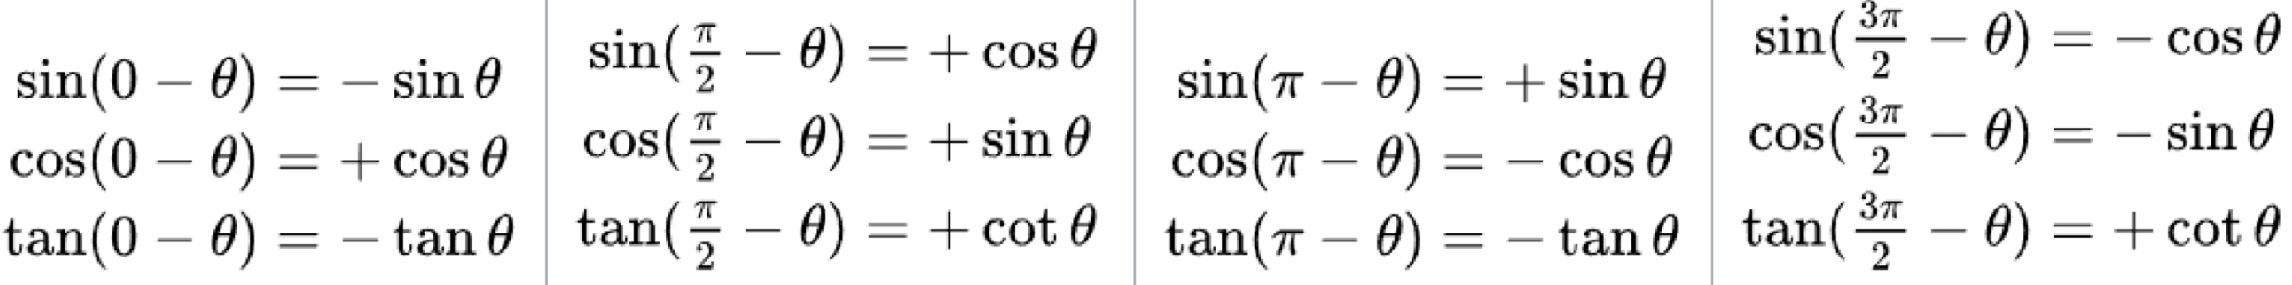
\includegraphics[width=\linewidth]{assets/prelude/trig-identities.pdf}


\noindent Students are often asked to solve problems by applying a subset of those rules, \eg, $sin(0 - \theta) = -sin(\theta)$.

\begin{figure*}[h]
    \centering
    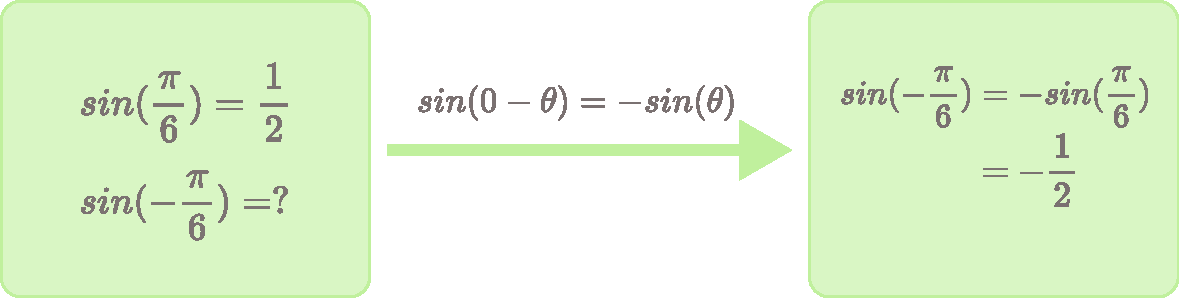
\includegraphics[width=0.75\linewidth]{assets/prelude/symbolic-transform.pdf}
    % \vspace{-10pt}
\end{figure*}

\setlength{\columnsep}{1em}
\setlength{\intextsep}{0em}
\begin{wrapfigure}{r}{.23\textwidth}
\vspace{-10pt}
  \begin{center}
    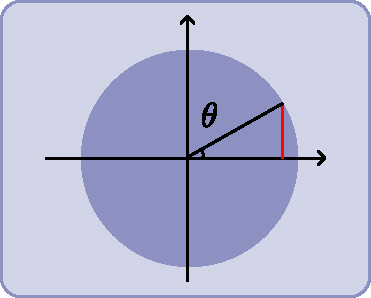
\includegraphics[width=0.23\textwidth]{assets/prelude/unit-circle.pdf}
  \end{center}
\end{wrapfigure}

A useful visual representation of this concept is the unit circle: on a Cartesian plane with a circle of radius $1$ centered at the origin, concrete values of trig functions are represented visually and rules are implicitly encoded as geometric transformations. For instance, the value of $sin(\theta)$ is the y-coordinate of a point on the circle, where the ray from the origin to the point forms angle $\theta$ with the x-axis.

To derive the identity rule visually, one only needs to note that $-\theta$ is a reflection about the x-axis, and observe that the y-coordinate is now a negative number. Instead of having to memorize a big set of rules, one can reduce this problem to a simple operation on the visual representation of a unit circle.

\vspace{10pt}
\begin{figure*}[h]
    \centering
    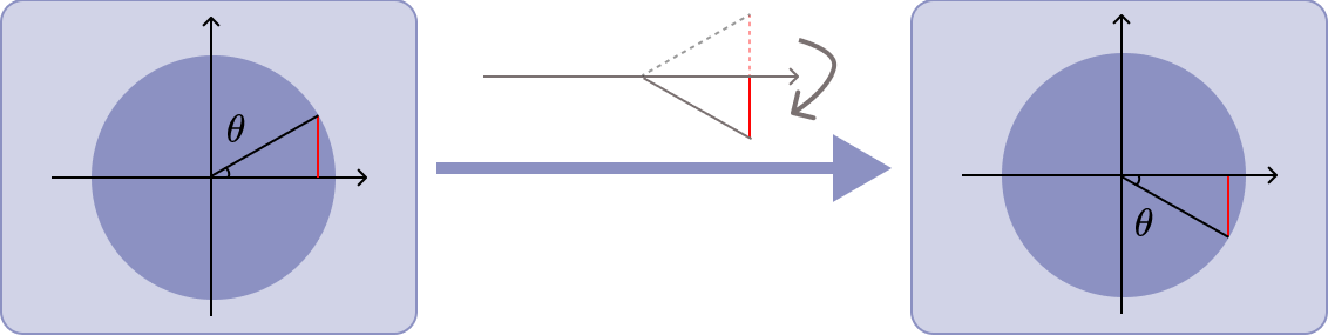
\includegraphics[width=0.70\linewidth]{assets/prelude/visual-transform.pdf}
    % \vspace{-10pt}
\end{figure*}

By translating the symbols to a visual representation, a unit circle, a student completely bypasses the tedious memorization of trig identities. While this is a much more retainable and robust representation for students, are we teaching representations like this to students? What does it take for students to internalize it? 

\chapter{Introduction}

``Mental pictures'' and ``visual intuition'' capture how people make sense of abstract concepts and see solutions to hard problems in a visual way. Hadamard described numerous examples of mathematicians doing exactly this in \emph{The Mathematician's Mind}~\cite{Hadamard1997a}, later summarized by Alan Kay~\cite{doingWithImages}:

\begin{quote}
Jacques Hadamard, the famous French mathematician, in the late stages of his life, decided to poll his 99 buddies, who made up together the 100 great mathematicians and physicists on the earth, and he asked them, ``How do you do your thing?'' They were all personal friends of his, so they wrote back depositions. Only a few, out of the hundred, claimed to use mathematical symbology at all. Quite a surprise. All of them said they did it mostly in imagery or figurative terms.
\end{quote}

Learning research suggests that visual representations of knowledge are powerful tools for thought. Visual representations like diagrams enable more robust learning \cite{multimediaLearning} and abstract and flexible problem solving~\cite{Koedinger1990a, pictureAlgebra, DiagramsThousandWords}. Importantly, when people work with visuals, they build better conceptual understanding and more flexible mental models that go beyond memorized procedures~\cite{multipleReps}.

\setlength{\columnsep}{1em}
\setlength{\intextsep}{0em}
\begin{wrapfigure}{r}{.45\textwidth}
\vspace{-10pt}
  \begin{center}
    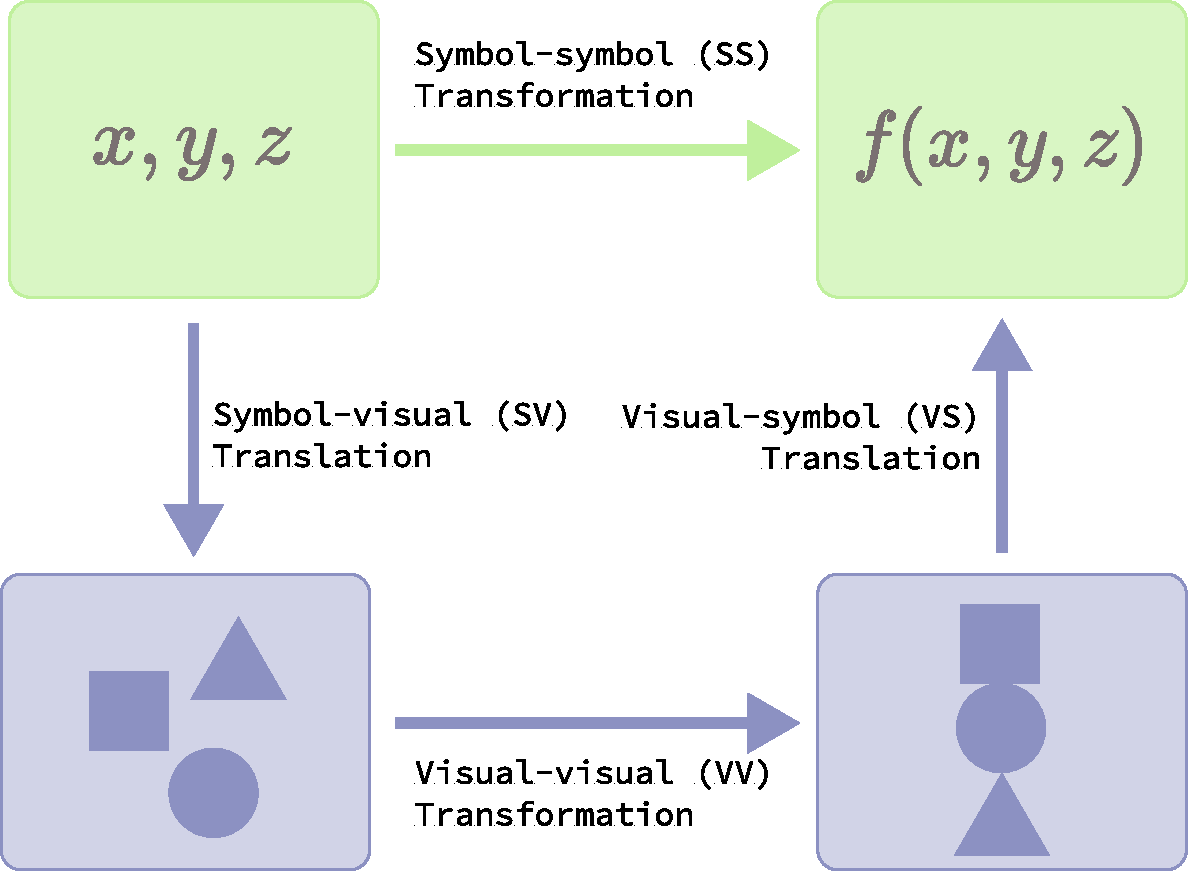
\includegraphics[width=0.45\textwidth]{assets/chapter-1/grounding-rectangle.pdf}
  \end{center}
\end{wrapfigure}

Let me use a diagram to capture this: the \textbf{grounding rectangle} represents two pathways to learning and problem solving: One can perform symbol-to-symbol transformations (SS, or “symbol pushing”) or through an \textcolor[HTML]{8C91C2}{alternative diagrammatic pathway}: a symbol-to-diagram translation (SV), a diagram-to-diagram transformation (VV), and finally a diagram-to-symbol translation (VS).

Research on expertise development suggests a need for substantial exposure involving repetition in varied contexts or deliberate practice \cite{deliberatePractice} to acquire the perceptual chunks \cite{chunkingModels, perceptualLearningExpertise} that support accurate interpretation and use of visual representations~\cite{Koedinger1990a}. Through enough practice, learning the two paths in the grounding rectangle can produce better, more robust memory \cite{dualCoding}, learning~\cite{multipleReps, multimediaLearning, cotraining}, and future reasoning, both in providing flexibility and in supporting error recovery \cite{groundedAndAbstractReps}.

In reality, there seems to be an over-abundance of symbolic practice, continuing Kay's train of thought:

\begin{quote}
    The sad part of the diagram is that every child in the United States is taught math and physics through this [symbolic] channel. The channel that almost no adult creative mathematician or physicist uses to do it... They use this channel to communicate, but not to do their thing.
\end{quote}

Diagrammatic practice is rare due to the significant cost of authoring diagrammatic problems. Existing diagramming tools often require hours of low-level tweaking of geometric primitives and do not capture the core task of diagramming: representing ideas visually. In other words, these tools lack \emph{representational salience}. As a result, the diagrams created by existing tools don't have semantics, as they are merely a collection of pixels and geometric blobs.  

% In prior work, colleagues and I built \Penrose, a diagramming platform that explicitly encodes visual representations in domain-specific languages (DSLs)~\cite{penrose}. In this thesis proposal, I argue that this explicit encoding can be leveraged to (1) reduce the programming effort of producing diagrammatic problems at scale and (2) simplify the workflow of authoring interactive diagrams. The resulting diagrams also carry rich semantics, and I propose to use them to (3) provide useful, automated feedback to students. My thesis statement summarizes the above:

% \vspace{10pt}
% \boxtext{
% \textbf{Encoding visual representations in diagramming tools simplifies programming of interactive visual activities that provide students with automated feedback at scale.}
% }
% \vspace{10pt}

% The expected contributions of this work are:

% \begin{enumerate}
%     \item \emph{Need-finding studies} on challenges authors face.
%     \item \emph{A platform of tools} based on the visual encoding of \Penrose for mass-production of diagrams (\cref{chp:edgeworth}) and rapid authoring of interactive diagrams (\cref{chp:ipenrose}).
%     \item \emph{A theoretical framework} of the grounding rectangle, which guides the design of tools presented in this proposal.
% \end{enumerate}

% \begin{proposed}
% \textbf{Note.} This proposal contains a mix of completed, in-progress, and proposed projects. In the rest of this document, proposed work will be marked in orange on the left margin. 
% \end{proposed}

\section{Research Questions}


%
\subsection{Hypotheses and research questions}

Comparing with related work discussed in \cref{sec:edgeworth-related}, \Edgeworth uniquely support scalable generation of diagrammatic translation problems in multiple domains. Therefore, in this section, I discuss hypotheses that cover the essential features of \Edgeworth such as the mutation-based approach and automatic detection of examples and counterexamples. For each hypothesis, I will also discuss further research questions to be investigated in the evaluation plan. 

\boxtext{\textbf{H1:} Given manageable effort in configuring the mutator, \Edgeworth can reliably generate examples and counterexamples for translation problems with relatively few mutants required.}

An effective translation problem needs to include both examples and counterexamples. Therefore, the technical approach of \Edgeworth---program mutations on \Substance code---must produce them reliably. To verify H1, the following research questions need to be answered:

\begin{itemize}
    \item \textbf{R1.1}: How many mutants does \Edgeworth need to generate to obtain sufficient examples and counterexamples for translation problems?
    \item \textbf{R1.2}: How frequently does \Edgeworth succeed or fail at doing so?
\end{itemize}

The preliminary evaluation showed that the mutator configuration will affect the quality of the mutants. Therefore, I will also address the following research question on mutator configuration and will use the results to further investigate possible ways to lower the configuration burden, e.g. the programming-by-example workflow and changes to the configuration format.

\begin{itemize}
    \item \textbf{R1.3}: How much configuration effort is required to produce examples and counterexamples? 
\end{itemize}

\boxtext{\textbf{H2}: \Edgeworth makes translation problem authoring more efficient.}

The main goal of \Edgeworth is to improve the efficiency of translation problem authoring. To verify H2, the evaluation plan will answer:
\begin{itemize}
    \item  \textbf{R2.1}: Comparing with workflows that authors are using, can \Edgeworth shorten the authoring time of translation problems?
    \item  \textbf{R2.2}: Which aspect(s) of the authoring workflow does \Edgeworth simplify, and does \Edgeworth introduce new authoring difficulties? 
    \item  \textbf{R2.3}: Are authors more efficient using the configuration-based workflow or programming-by-example workflow?
\end{itemize}

Regardless of the answer to R2.1, meaningful results on R2.2 can provide more insights on how \Edgeworth's approach impacts the problem authoring experience. For instance, I postulate that \Edgeworth improves authoring efficiency by (1) simplifying the mechanics of diagram production and (2) reducing the author's effort to come up with examples and counterexamples. On the other hand, \Edgeworth's mutation-based approach may introduce new problems such as difficulties finding the right diagrams from the mutant pool and controlling the quality of examples. The automatic detection heuristics described above aim to mitigate these difficulties.

\boxtext{\textbf{H3}: \Edgeworth can automatically distinguish examples from counterexamples, and this feature helps authors find examples and counterexamples for translation problems.}

The effectiveness of translation problems depends on the choice of examples and counterexamples. I hypothesize that example generation/selection is a nontrivial activity that authors spend time doing, and computational support in \Edgeworth can help authors identify examples/counterexamples. Answering the following research questions will verify H3:

\begin{itemize}
    \item \textbf{R3.1}: Can \Edgeworth automatically detect examples, counterexamples, and edge cases with a reasonably high accuracy?
    \item \textbf{R3.2}: Do the detection results help authors identify potential answers to translation problems?
\end{itemize} \subsection{Limitations}


All the work presented in this proposal was carried out in collaboration with others, and to recognize this, I use ``we'' rather than the singular first person in the subsequent chapters.


\chapter{Background and Related Work}
\label{chp:background}
\begin{figure}[h]
    \centering
    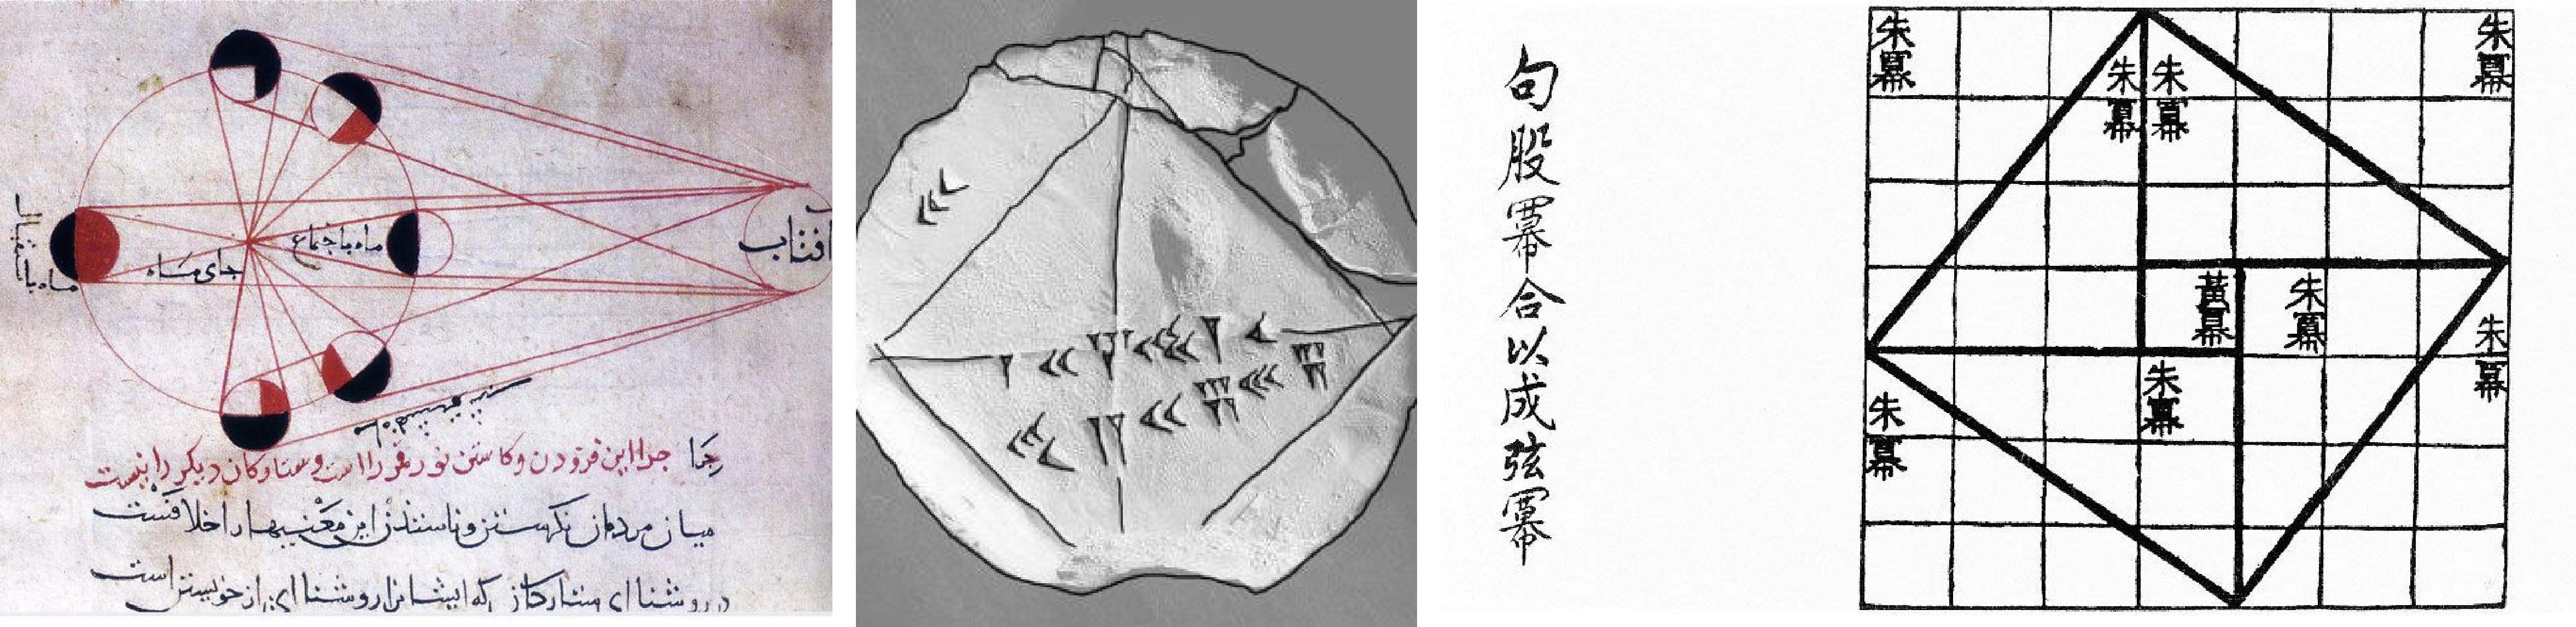
\includegraphics[width=\linewidth]{assets/related-work/historical-diagrams.pdf}
    \caption{Several examples of ancient diagrams, from left to right: (1) Phases of the Moon: Abu Rayhan Muhammad ibn Ahmad al-Biruni (Iranian, 973-1048), (2) Babylonian clay tablet diagramming an approximation of $\sqrt{2}$ (1900 -1700 BCE), and (3) Geometric proof of the Pythagorean theorem in Zhoubi Suanjing 周髀算经 (1st century BCE).}
    \label{fig:ancient-diagrams}
\end{figure}

This chapter provides background on diagrams in general, existing diagramming tools, and research on using diagrams for learning.

\section{Diagrams}
\label{sec:diagrams}

\citet{tversky_diagrams_2017,tversky_visualizing_2011} defines diagrams as \quotei{an arrangement of marks on a virtual page (stone, paper, or screen) that represents a set of ideas and their relations}. This definition is broad enough to include many ancient and modern graphical representations of ideas, including graphs, charts, infographics, and many more. Under this definition, diagrams are perhaps one of the oldest form of human communication and expression. For instance, \cref{fig:ancient-diagrams} shows a few examples of diagrams in ancient times around the world. Although there are many more definitions of diagrams (for example, \cite{bender_culture_2010,card_readings_1999,infographics,arnheim_visual_1969,tufte1983visual}), this chapter does not aim to provide a comprehensive discussion of how diagrams are defined. Rather, we examine two aspects of a diagram to motivate the types of graphics this dissertation focuses on: content and utility.

First, this dissertation contribute tools (\cref{chp:penrose,chp:edgeworth}) that produce diagrams that depict logical, non-quantitative \textit{concepts}, rather than quantitative \textit{data}. As we will discuss in \cref{sec:related-systems,chp:interviews}, this focus on conceptual diagrams is largely driven by the relative dearth of tools for making conceptual diagrams. In contrast, statistical graphics~\cite{wilkinson_grammar_2012} largely depict quantitative data, and are well supported by authoring tools~\cite{d3, vega}. 

The second aspect is the utility of diagrams, which set them apart from decorative paintings, photos, floor plans, and more. \citet{designWithDiagrams} distinguishes between \emph{pictorial} and \emph{propositional} graphics: instead of directly visualizing data or depicting naturalistic scenes, diagrams (propositional graphics in \citeauthor{designWithDiagrams}'s terms) ``constitute knowledge and embody media-independent abstractions for inference-making.'' The specific utility of diagrams for inference-making is significant enough to prompt psychologists and cognitive scientists to study their role in problem-solving and learning. Diagrams have been shown to have cognitive benefits to reasoning and problem-solving~\cite{whyDiagramWorth, koedinger_emergent_1992, mayer_multimedia_2002}. Compared to textual representations, diagrams facilitate fast recognition and direct inference by making the most relevant information explicit and easily findable~\cite{whyDiagramWorth}. As an external representation of abstract structures of tasks, diagrams can work together with one's mental representation and are an indispensable part for accomplishing distributed cognitive tasks~\cite{DistributedCognitive}. Akin to \citet{designingWithDiagrams}, \citet{hegarty_types_1999} distinguish between \emph{pictorial} and \emph{schematic} visual representations and show that schematic representations of relative spatial relationships significantly outperform pictorial ones that encode visual appearances.
In addition to their values as an external, static representation of knowledge, diagrams are also beneficial when people learn \emph{with}, instead of \emph{from} them~\cite{tippett_what_2016}. In educational contexts, explicit training of drawing, including the creation of new visual representations and adoption of new ones, significantly improve students' ability to work with multiple representations and improve learning, reasoning, and communication skills~\cite{ainsworth_drawing_2011}. Moreover, creating diagrams as visual explanations also improves learning, since they can act as a check for completeness and a medium for inference~\cite{bobek_creating_2016}. 

% In general, people do not need formal training in visual design to create and interpret effective diagrams and learners at all levels can benefit tremendously from creating diagrams~\cite{ABC}.

Beyond diagrams' utility for more efficient cognitive inference and learning, logicians, mathematicians, and philosophers have argued for diagrams' fundamental role in reasoning. Historically, diagrams were often dismissed as mere illustrations---supplementary tools rather than central components of logical arguments. This traditional view has been predominantly influenced by the dominance of symbolic languages in the history of logic, where precision and formal rigor were prioritized over visual representation~\cite{shin_diagrams_2018}. Peirce's existential graphs~\cite{peirce_collected_1931} are a form of diagrammatic logic that he argued could represent logical relations in a manner both clearer and more intuitive than traditional symbolic logic. Peirce believed that existential graphs could express logical relationships with a degree of generality and precision that rivals, if not surpasses, that of symbolic logic, particularly in their ability to represent the continuity of logical processes. Jon Barwise and John Etchemendy's work on the importance of diagrams in logical reasoning~\cite{barwise_visual_2019} aligns closely with the earlier insights of Peirce. Peirce's existential graphs, which visually represent logical propositions and their relationships, serve as a precursor to Barwise's concept of ``heterogeneous reasoning,''~\cite{barwise_heterogeneous_1993} where visual and symbolic methods are integrated to solve logical problems more effectively. 


% In addition to knowledge representation, conceptual diagrams are also a medium for creativity and exploration, since they do not require early commitments to design decisions and focus on the \emph{form} of possible solutions~\cite{ConceptualArchDesign}.

% TODO: diagrams generate information

% \subsection{Cognitive benefits of diagrams for learning and problem-solving}
% \label{sec:diagram-benefits}

\section{Learning how to use diagrams}


Whether for more efficient problem-solving or logical reasoning, one must learn how to use diagrams properly. At the end of \citetitle{whyDiagramWorth}, \citet{whyDiagramWorth} noted that:

\begin{quote}
[D]iagrams are useful only to those who know the appropriate computational processes for taking advantage of them. Furthermore, a problem solver often also needs the knowledge of how to construct a ``good'' diagram that lets him take advantage of the virtues [of diagrams] we discussed.~\cite[p.~99]{whyDiagramWorth}
\end{quote}

In this section, we provide background on why students need to practice for better fluency in visual representations and how diagram variations may help students practice using them more effectively. 

\subsection{Representational fluency and contrasting cases}

Representational fluency refers to the ability to quickly understand a visual representation and to use it to solve domain-specific tasks~\cite{multipleReps}. To become representationally fluent, an important first step is to identify meaningful aspects of a particular representation. \citet{kellman_perceptual_2010} show that mapping between symbolic and visual representations leads to intuitions about the way equivalent structures relate to each other. The learning that results from constructing connections between symbols and diagrams can be more flexible. Students are better at transferring their learning from the problems they have explicitly practiced to more open-ended problems and their conceptual understanding is better~\cite{25learning}. 

In addition to mapping between representations, \citet{marton_sameness_2006} also showed that contrasting cases help students discern crucial parts of a particular representation. Early on, students benefit from discerning instances and noninstances that differ in only one dimension of variation. As students become more fluent, a \emph{fusion} of multiple varying dimensions in problems may be necessary~\cite{chik_simultaneity_2004}. \citet{arnheim_visual_1969} characterized this need for many diagrams (or animation of diagrams) in \citetitle{arnheim_visual_1969}:

\begin{quote}
The usual illustrations in textbooks and on the blackboard help to make a problem visible, but they also freeze it at one phase of the range to which the proposition refers. Therefore, they tempt the student to mistake accidental circumstances for essential ones. The solution is not to leave out illustrations but either to produce mobile models\dots{} or, at least, to use immobile illustrations in such a way that the student realizes which of their dimensions are variables. ~\cite[p. 182]{arnheim_visual_1969}
\end{quote}

\subsection{Multiplicity of examples}

Indeed, in addition to training representational fluency, multiple examples and repeated, varied practice are well-documented strategies for broader learning goals in the learning science literature. Many studies have demonstrated substantial science, technology, engineering, and mathematics (STEM) learning benefits for multiple worked examples per topic \cite{pashler_organizing_2007}. Equally important is research indicating the importance of active learning \cite{chi_icap_2014,deslauriers_measuring_2019} and repeated practice \cite{deliberatePractice,schnackenberg_learner_1998} that occurs within varied contexts \cite{PV94,rohrer_shuffling_2007} and involves direct explanatory feedback \cite{kellman_perceptual_2010}.

\citet{rau_conditions_2017} reports that, unfortunately, providing computational support for representational fluency is time-consuming with current tools. Our formative study (\cref{sec:edgeworth-formative}) confirmed this claim and revealed barriers resulting from the limitations of diagram authoring tools. To address these limitations, \Edgeworth (\cref{chp:edgeworth,chp:edgeworth-eval}) aims to simplify the workflow for creating diagram variations for repeated practice. 


\section{Digital diagramming tools}
\label{sec:related-systems}

% Intro
As this dissertation investigates diagram authoring empirically (\cref{chp:interviews}) and contributes a new diagramming tool (\Penrose, \cref{chp:penrose}), we survey existing digital tools for making diagrams. Although many diagramming tools support both text-based and graphical interfaces, we categorize current diagramming tools by their dominant mode of interaction: programming-language based (PL) tools and direct manipulation (DM) tools. 

% Programming languages: DSL, general purpose
We use PL tools to refer to text-based diagramming tools, including imperative or declarative programming languages, libraries, frameworks, and embedded domain-specific languages. General-purpose tools such as Processing~\cite{Reas:2006:PPM}, Asymtote~\cite{Bowman:2008:AVG}, PGF/TikZ, and Paper.js\footnote{\url{http://paperjs.org/}} provide program constructs that model graphical primitives and operations akin to those in Scalable Vector Graphics (SVG)~\cite{SVGStandard}. Many of their shared disadvantages are well summarized in TikZ's manual~\cite{TikZ-Manual}: ``steep learning curve, no WYSIWYG, small changes require a long recompilation time, and the code does not really ``show'' how things will look like.'' Domain-specific tools allow diagram specifications that are higher-level and specialized to the problem domain to smoothen the learning curve. They are developed either from scratch (\eg~GraphViz and the DOT language for graph visualization~\cite{Graphviz}) or on top of general-purpose tools (\eg~TikZ's extensions, \texttt{tkz-euclide} for Euclidean geometry). However, many of them still inherit the other disadvantages from above. 

DM tools represent interactive diagramming tools that support WYSIWYG interfaces and direct interaction with shapes. Akin to PL tools, general-purpose DM tools such as Adobe Illustrator, Inkscape, and Figma also have similar sets of primitives, but often provide a large number of widgets or drawing tools (\eg~Illustrator CC has nearly 100 built-in tools\footnote{\url{https://helpx.adobe.com/illustrator/user-guide.html}}). To overcome the disadvantage of their highly manual interaction model, both Illustrator and Inkscape provide language bindings or command-line tools for automation, but they still suffer from the above problems of PL tools. Popular domain-specific diagramming tools such as draw.io and Gliffy are template editors that provide predefined, mostly box-and-arrow style shapes, limiting users to a narrow set of diagrams. Research prototypes such as Sketchpad~\cite{sketchpad} and ThingLab~\cite{thinglab} automate diagram layout using constraint solving, but many edit actions like selection and shape construction remain manual. Other prototypes like Apparatus\footnote{\url{http://aprt.us/}} and Bret Victor's dynamic visualization tool~\cite{dynamicViz} incorporate some limited programmatic operations (\eg~macro recording, variable declaration, and computed properties) via direct interactions. 

% 3 Wave of data visualization: the point is, diagramming tools haven't caught up with the dataviz trend
% Statement of our goals
As discussed by \citet{satyanarayan_critical_2020}, data visualization tools have transformed over the past decade. The major advances are characterized by three ``waves'': (1) improvement of individual charts' quality, (2) theories and tools that enable mass-production of visualizations, and (3) the convergence of tools~\cite{thirdWaveViz}. Whereas the benefits of conceptual diagrams are clear and theoretical foundations exist, most of the diagramming tools are still not easily scalable and there are large gaps in existing technologies, notably between PL and DM tools. In other words, the \nth{2} wave of conceptual diagramming is still not here. In the interview study presented in \cref{chp:interviews}, we aim to gain a deep understanding of people's diagramming process to drive the design of tools that fill these gaps.



% \subsection{Empirical studies on diagramming-related activities}

% Although conceptual diagrams are widely studied as a powerful visual representation in multiple domains, there has not been a significant amount of prior work that focuses on the \emph{authoring} of conceptual diagrams, especially with digital tools. 

% However, prior work in related activities such as note-taking and whiteboarding suggests some insights for both understanding these activities and opportunities for tool design. Studies on sketches in STEM~\cite{Whiteboards} and software engineering~\cite{Whiteboards-Ko} suggest a need for automating the process of sketching and preserving transient sketches such as whiteboard drawings with appropriate tools. In similar activities such as annotating documents, personal annotations undergo dramatic changes such as significant substantiation and clarification when they are shared on public platforms~\cite{Annotations}. Digitization of the analog pen-and-paper interface attempts to make the transformation process smoother. While digital ink tools imitate the pen-and-paper experience and provide more versatility and power, there still exist gaps between the manual and digital experience of sketching due to conflicting affordances of analog pen and digital ink~\cite{AsWeMayInk}. 

% Given the lack on the prior work on this topic, \cref{chp:interviews} directly investigates the process of creating conceptual diagrams using digital tools.

 

% %%%%%%%%%%%%%%%%%%%%%%%%%%%%%%%%%%%%%%%%%%%%%%%%%%%%%%%%%%%%%%%%%%%%%%%%%%%%%%%% Not used


% % User-centered design is good
% % Recent research demonstrated significant usability and efficiency gains when empirical data are used to motivate tool design. For instance, Playful Palette~\cite{PlayfulPalette} addresses visual artists' needs elicited from a pilot user study and showed effectiveness by increasing the usage of distinct colors by 39\% and amplifying artists' creativity. The design of Data Illustrator was informed by intensive interviews with graphic designers and the result was a tool that enhanced users abilities to compose visualizations~\cite{DataIllustrator}. Our goal in this paper is to study the process of creating conceptual diagrams to drive the design of tools that support this process. 


% % \subsection{Empirical studies on diagramming-related activities}

% % \todoi{go through this section again and consider removing it}

% % Empirical studies on diagramming and related domains have revealed cognitive and behavioral patterns of how people interact with external representations such as diagrams and notes. These findings inform our study of how domain experts create conceptual diagrams.

% % Grammel \etal{} found that, When making information visualizations, novices tend to operate on higher-level constructs in both the data and visual spaces: they prefer to operate on their high-level mental models of the data rather than data attributes; they also tend to use composite visual constructs (\eg~bars and tree nodes) rather than primitives (\eg~polygons and circles)~\cite{NoviceInfoviz}. 

% % % Do domain experts, who have a better grasp of the semantic meaning of data, use similar generic visual constructs? In this study, we investigate how conceptual diagrammer find and construct high-level representations to aid their thinking. 

% % Studies on sketches in STEM~\cite{Whiteboards} and software engineering~\cite{Whiteboards-Ko} suggest a need for automating the process of sketching and preserving transient sketches such as whiteboard drawings with appropriate tools. In similar activities such as annotating documents, personal annotations undergo dramatic changes such as significant substantiation and clarification when they are shared on public platforms~\cite{Annotations}. Digitization of the analog pen-and-paper interface attempts to make the transformation process smoother. While digital ink tools imitate the pen-and-paper experience and provide more versatility and power, there still exist gaps between the manual and digital experience of sketching due to conflicting affordances of analog pen and digital ink~\cite{AsWeMayInk}. In this paper, we investigate the process of transforming sketches to digital, formal versions. 

% % Penrose

% \subsection{Diagramming Systems}
% \label{sec:RelatedSystems}

% Here we consider how our system design relates to other systems that convert abstract mathematical ideas into visual diagrams.  Other classes of tools, such as general-purpose drawing tools (\eg{}, \emph{Adobe Illustrator}) can also be used to make diagrams, though one quickly runs into barriers, such as for large-scale diagram generation or evolving the style of a large collection of existing diagrams.  A broader discussion of related work can be found in a pilot study we did on how people use diagramming tools~\cite{Ni:2020:HDE}.

% There are three main kinds of systems that convert an abstract form of input (\eg{}, an equation or code) into a visual representation.  Language-based systems, such as \textit{TikZ}~\cite{TikZ-Manual} (which builds on \TeX), are domain-agnostic and provide significant flexibility for the visual representation. Their use of ``math-like'' languages influenced the design of \Substance.  However, existing systems do not aim to separate mathematical content from visual representation. For instance, TikZ is domain- and representation-agnostic because it requires diagrams to be specified at a low level (\eg{}, individual coordinates and styles) making programs hard to modify or reuse.  Moreover, since there are only shallow mathematical semantics, it becomes hard to reason about programs at a domain level.

% Plotting-based systems, like \emph{Mathematica} and \emph{GeoGebra}~\cite{geogebra5} enable standard mathematical expressions to be used as input and automatically generate attractive diagrams.  Just as a graphing calculator is easy to pick up and use for most students of mathematics, these tools inspired us to provide a ``tiered'' approach to \Penrose{} that makes it accessible to users with less expertise in illustration (\figref{NoviceExpertUsers}). However, much like a graphing calculator, the visual representations in these systems are largely ``canned,'' and the set of easily accessible domains is largely fixed.  For instance, \emph{Mathematica} does not permit user-defined types, and to go beyond system-provided visualization tools, one must provide low-level directives (in the same spirit as tools like \textit{TikZ}).

% Finally, systems like \emph{graphviz}~\cite{Graphviz}, and \emph{Geometry Constructions Language}~\cite{Janivcic:2006:GCLC} translate familiar domain-specific language into high-quality diagrams. Here again, the domains are fairly narrow and there is little to no opportunity to expand the language or define new visualizations.  Yet the convenience and power of such systems for their individual domains inspired us to build a system with greater extensibility. More broadly, while all these systems share some design goals with ours, a key distinction is that \Penrose\ is designed from the ground up as an extensible \emph{platform} for building diagramming tools, rather than a monolithic end-user tool.


% % Edgeworth


% \section{Background and Related Work}


\section{Tools for Problem Generation}
\label{sec:problem-generation}

In addition to making standalone diagrams, this dissertation also covers diagrammatic problem authoring with \Edgeworth in~\cref{chp:edgeworth,chp:edgeworth-eval}. In this section, we cover related digital systems for practice problem generation in general, and their support for diagram authoring. \citet{kurdi_systematic_2020} conduct a systematic review of automatic problem generation tools and show that the majority of tools address language learning. In this section, we focus on problem generation tools in STEM learning and discuss how they relate to diagrammatic problem generation and \Edgeworth. 

Intelligent Tutoring Systems (ITS) are automated curricula that include practice problems with personalized feedback (\emph{inner loop}) and customize problem selection to improve students' performance (\emph{outer loop})~\cite{vanlehn_behavior_2006}. Problem banks are an important component of ITS tools, so many systems have built-in authoring support to generate a large number of problems via templating. For instance, Cognitive Tutor Authoring Tools (CTAT) is an ITS authoring platform~\cite{aleven_cognitive_2006}. CTAT has a ``Mass Production'' feature that lets the user create a problem template and insert problem-specific values via a spreadsheet~\cite{aleven_rapid_2006}. Similarly, the ASSISTment builder allows authors to ``variabilize'' numerical values in problem templates for automatic generation~\cite{ASSISTment}.  

In the context of testing, researchers proposed systems that generate test problems (\emph{items}) automatically for adaptive testing and cost-effectiveness~\cite{gierl2012automatic}.  Due to the need for numerous test items, automatic item generation systems also rely on templating (\emph{item models}) to generate items~\cite{gierl_role_2012,HOLLING200971,CheckIt}. For instance, IGOR~\cite[Chapter~13]{gierl2012automatic} has a similar approach to templating as CTAT and ASSISTment. While the templating approach is suitable for symbolic problems, they do not automate diagram generation. Authors still need to provide individual diagrams in templates in CTAT, ASSISTment, or IGOR. 

In \cref{chp:edgeworth}, we present \Edgeworth, which complements these tools by enabling authors to automate diagram variation production. Diagrammatic problems generated by \Edgeworth can be integrated into problem banks and managed by the outer loop of ITS for an adaptive learning experience. \Edgeworth does not currently support template variables in the textual prompt or diagram labels. However, it is possible to parameterize the example diagram as a problem template and use existing template-based systems to generate problem variations. 

Other problem generation systems employ different methods from templating. A number of systems use \emph{program synthesis} to synthesize a program that produces many problem instances~\cite{gulwani_example-based_2014}.  \citet{singh_automatically_2012} generate algebraic equality proof problems from example problems. \citet{machineTeaching} speed up ITS authoring in CTAT by synthesizing ITS problems from user demonstration of problem solutions. \citet{andersen_trace-based_2013} model procedures to solve algebra problems as imperative programs and use execution traces of these programs to generate a series of problems. Notably, \citet{gulwani_synthesizing_2011} generate solutions to geometry drawing problems by synthesizing programs of ruler-and-compass geometry constructions from a program specification. Though not strictly a problem generation tool, the generated solutions can be illustrated diagrammatically. However, the approach in \cite{gulwani_synthesizing_2011} is specific to the domain of geometry, whereas \Edgeworth's approach is domain-agnostic. Synthesis-based systems often have an advantage of a simpler user experience, since the author can provide examples and the tool automates problem generation itself. The approach of \Edgeworth takes inspiration from these tools in that \Edgeworth only requires the author to provide one example diagram. However, \Edgeworth does not need to generate programs from a specification. It merely performs mutations on an example diagram. 

Commonly used in human intelligence tests and as computer vision benchmarks, Figural Analogy Problems (FAPs) give a series of diagrams and ask the respondent to infer or select the next diagram given some patterns in the given diagrams~\cite{yang_automatic_2022}. Early automatic FAP generators were based on human-crafted shape composition rules~\cite{hornke_rule-based_1986} and cognitive models~\cite{embretson_cognitive_1998}. Newer systems~\cite{wang_automatic_2015,pmlr-v80-barrett18a} encode variation rules~\cite{carpenter_what_1990} as first-order logic constraints. While FAPs are by definition highly diagrammatic, FAPs focus on pure visual reasoning, while in STEM problems often focus on mapping symbolic notations to visuals. Moreover, diagrams in STEM are much more diverse due to the multitude of disciplines, and are not limited by a few variation rules. That said, \Edgeworth takes inspiration from FAP generators' rule-based approach. However, \Edgeworth's mutations are domain-agnostic and operate on logical objects, not fragments of the diagram itself.


\chapter[Understanding the Diagramming Process]{Understanding the Diagramming Process\footnote{This chapter is adapted from \citetitle{naturalDiagramming}~\cite{naturalDiagramming}.}}
\label{chp:interviews}

\chapter{Understanding the diagramming process and encoding visual representations}
\label{chp:interviews}

Before diving into the educational context, it's important to understand why creating diagrams is hard in the first place. This chapter discusses an interview study on how domain experts including educators use diagramming tools~\cite{naturalDiagramming}, and briefly shows how this study informs the design of \Penrose, the technical basis for tools presented in this proposal. 

\section{How domain experts create diagrams and implications for tool design}
\label{sec:naturalDiagramming}

Existing diagramming tools stand in tension between: a) General-purpose drawing tools such as Illustrator and Figma that offer simple pen-and-canvas or box-and-arrow metaphors, but are viscous~\cite{cognitiveDimensions}---users must constantly commit to exact positions, sizes, and styling of shapes. b) Dedicated diagramming tools such as Lucidchart and Gliffy that allow rapid changes, but rely heavily on templates, limiting diagrammers to a fixed set of visual representations. This relatively limited support for diagramming in tools is in part because the process of diagramming is poorly understood. For instance, how do diagrammers utilize the strengths and cope with the limitations of their tools? Which tools are chosen for what purposes?  Such a detailed understanding of the process can help design interactive tools to support diagramming.

I conducted interviews with 18 domain experts from a wide variety of disciplines such as math, computer science, architecture, and education. The interviews reveal that diagrammers have diverse interactions with visual representations in both physical sketches and digital tools, including finding, creating, storing, and reusing representations. 

One implication of our results is the opportunity to design tools informed by the processes of diagramming, and practices that domain experts already use, making digital diagramming more intuitive and efficient. Here are four key opportunities for natural~\cite{naturalProgramming} diagramming tools that allow diagrammers to express their ideas visually the same way they think about them:

\begin{itemize} 
    \item \textit{Exploration support}: supporting exploratory behaviors such as undo and backtracking during both abstract-level, breath-first exploration of the design space and low-level refinements of visual details.
    \item \textit{Representation salience}: allowing explicit creation and management of visual representations, \ie, the \emph{mappings} from domain constructs to shapes instead of geometric primitives themselves.
    \item \textit{Live engagement}: providing diagrammers with the sense of agency by designing for liveness and directness of the diagramming experience. 
    \item \textit{Vocabulary correspondence}: enabling diagrammers to interact with their diagrams using vocabularies that is conventional in their domain.
\end{itemize}


\chapter[\Penrose: From Notations to Beautiful Diagrams]{\Penrose: From Notations to Beautiful Diagrams\footnote{
This chapter is adapted from ``\citefield{penrose}{title}''~\cite{penrose}.}}
\label{chp:penrose}

\begin{teaserfigure}
  \centering
\begin{minipage}{150pt}
   % @keenan: lstlisting breaks inside the "teaserfigure" environment...
   % ...using a hack instead!
   \texttt{\textbf{Point} p, q, r, s} \\
   \texttt{\textbf{Segment} a := \{p, q\}} \\
   \texttt{\textbf{Segment} b := \{p, r\}} \\
   \texttt{\textbf{Point} m := \textbf{Midpoint}(a)} \\
   \texttt{\textbf{Angle} theta := $\angle$(q, p, r)} \\
   \texttt{\textbf{Triangle} t := \{p, r, s\}} \\
   \texttt{\textbf{Ray} w := \textbf{Bisector}(theta)} \\
   \texttt{\textbf{Ray} h := \textbf{PerpendicularBisector}(a)} \\
\end{minipage}\hspace{.25in}
\begin{minipage}{328pt}
   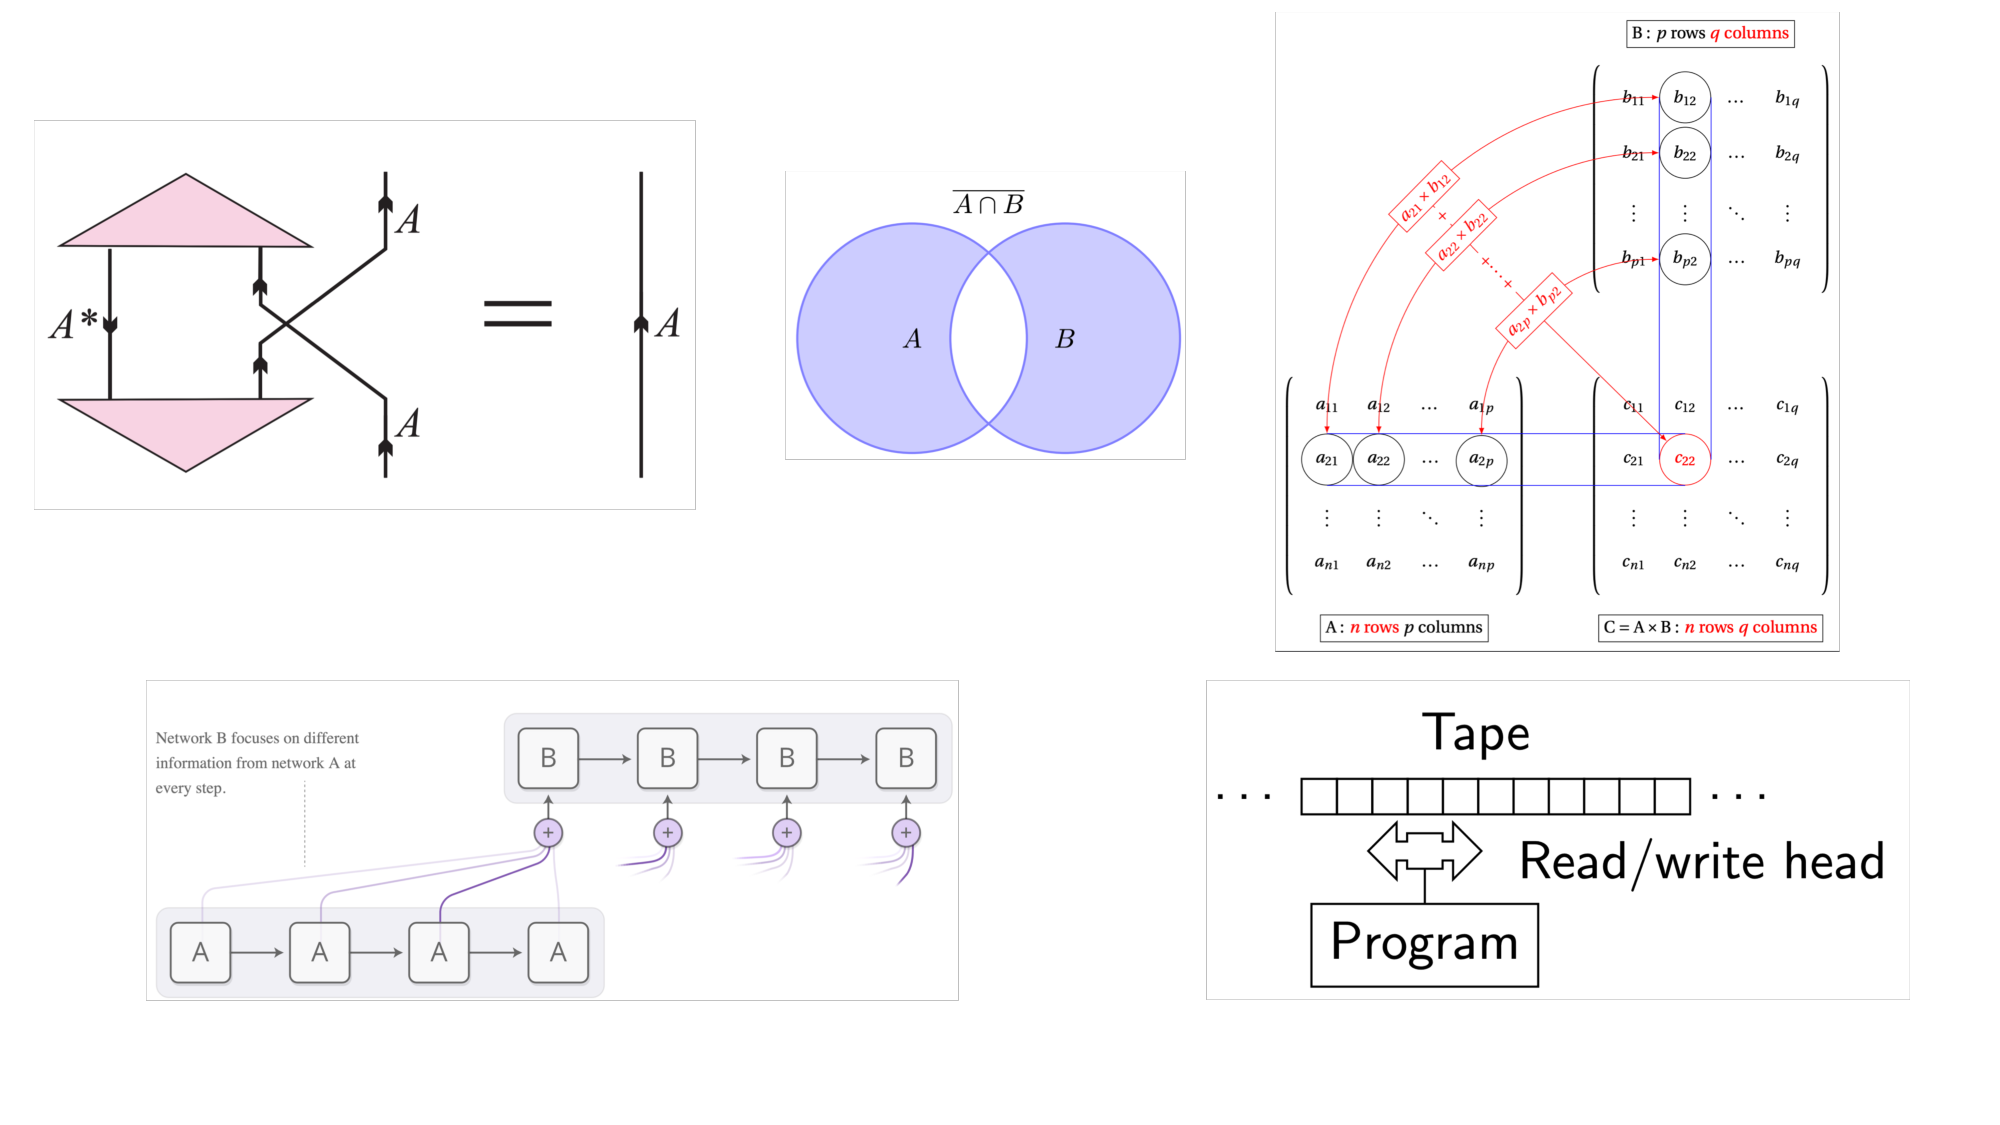
\includegraphics{penrose/teaser.pdf}
\end{minipage}
   \caption{\Penrose{} is a framework for specifying how mathematical statements should be interpreted as visual diagrams.  A clean separation between abstract mathematical objects and their visual representation provides new capabilities beyond existing code- or GUI-based tools.  Here, for instance, the same set of statements \figloc{(left)} is given three different visual interpretations \figloc{(right)}, via Euclidean, spherical, and hyperbolic geometry. (Further samples are shown in \figref{GeometrySamples}.)
     \label{fig:teaser}
   }
\end{teaserfigure}

Informed by the results from the interview study, colleagues and I have developed \Penrose, a language-based diagramming platform~\cite{penrose}. The core \Penrose system addresses \textbf{representation salience} and \textbf{vocabulary correspondence}: it has first-class support for creating and reusing visual representations and translates familiar math-like notation into one or more possible visual representations. To accomplish this, \Penrose decomposes the concerns of diagramming into two domain-specific languages (DSLs) with distinct purposes: \colorbox[HTML]{E7F3E7}{\Substance} contains the mathematical content in math notation. \colorbox[HTML]{DDDEED}{\Style} explicitly specifies mappings from mathematical objects to visual icons. 

% \setlength{\columnsep}{1em}
% \setlength{\intextsep}{0em}
% \begin{wrapfigure}{r}{.45\textwidth}
% \vspace{-10pt}
%   \begin{center}
%     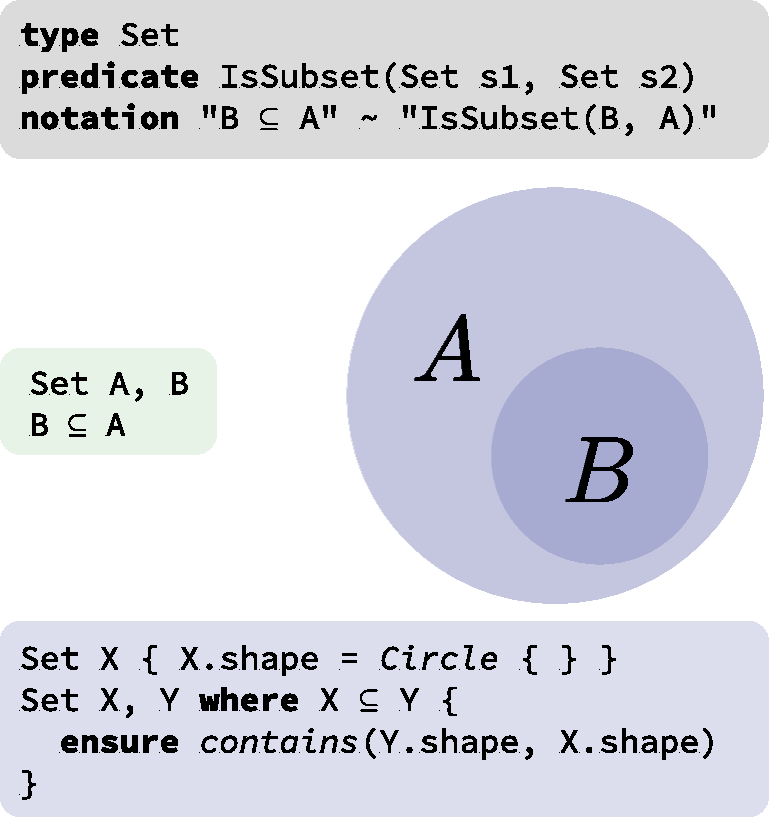
\includegraphics[width=0.45\textwidth]{assets/chapter-2/penrose-trio.pdf}
%   \end{center}
% \end{wrapfigure}

% Instead of a limited focus on one specific domain (as in GraphViz~\cite{graphviz} for graph theory or GroupExplorer~\footnote{\url{https://github.com/nathancarter/group-explorer}} for group theory), \Penrose is extensible to user-defined domains of diagramming. Both \Substance and \Style are parametrized by a \colorbox[HTML]{DBDBDB}{\Domain} schema that defines all possible objects (\eg, \sub{Set}) and relations (\eg, \sub{IsSubset}) in a particular domain, which can be used by associated \Substance and \Style programs. In addition to user-extensibility, a formally encoded domain also enables automatic generation of \Penrose diagrams. 

% \Penrose compiles a \textbf{trio} of \Domain, \Substance, and \Style into a constrained optimization problem defined by a set of graphical constraints (\eg, arrows that represent vectors should start from the origin). The optimization problem is in standard form, \ie, minimization of an objective function subject to equality and inequality constraints~\cite{convexOptimization}. Such problems may be solved with many standard methods. \Penrose currently uses an exterior point method~\cite{exteriorPoint} that starts with an infeasible point and pushes it toward a feasible configuration via progressively stiffer penalty functions---mirroring a process often used by hand.

% The design of \Penrose is driven by the design goals of reuse and scalability, and therefore is suitable for large-scale generation of visual content. The system is scalable and reusable in several dimensions:
    
% % \setlength{\columnsep}{1em}
% % \setlength{\intextsep}{0em}
% % \begin{wrapfigure}{r}{.45\textwidth}
% % \vspace{-10pt}
% %   \begin{center}
% %     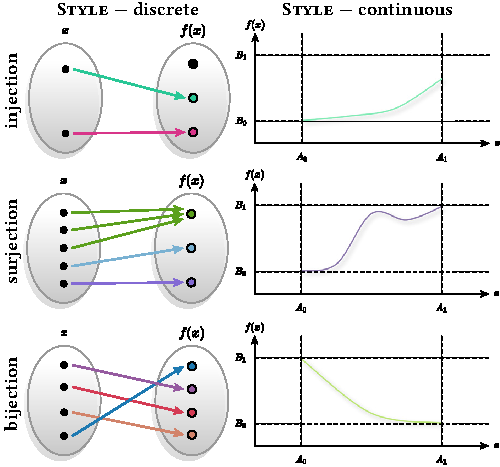
\includegraphics[width=0.45\textwidth]{assets/chapter-2/func-continuous-discrete-vert.pdf}
% %   \end{center}
% % \end{wrapfigure}

% \vspace{1em}
% \begin{figure}[h]
% \begin{minipage}[b]{0.48\linewidth}
% $\bullet$ The optimization problem produced by \Penrose often has multiple solutions, and each point in the solution space corresponds to an alternative diagram. No program changes are required to generate these alternatives.
%     \vspace{3pt}

% $\bullet$ For a visual representation encoded by a \Style program, a wide range of notations (\ie, \Substance programs) can be visualized without any changes to \Style. In the figure on the left, a single discrete \Style program is used to visualize three \Substance programs that describe injective, surjective, and bijective functions.
%     \vspace{3pt}

% $\bullet$ Conversely, multiple \Style{} programs can be applied to the same \Substance{} program, generating alternative visual representations of the same underlying entities. The \Substance programs in the figure are also visualized by an alternative continuous \Style.
% \end{minipage}
% \hfill
% \begin{minipage}[b]{0.5\linewidth}
%     \centering
%     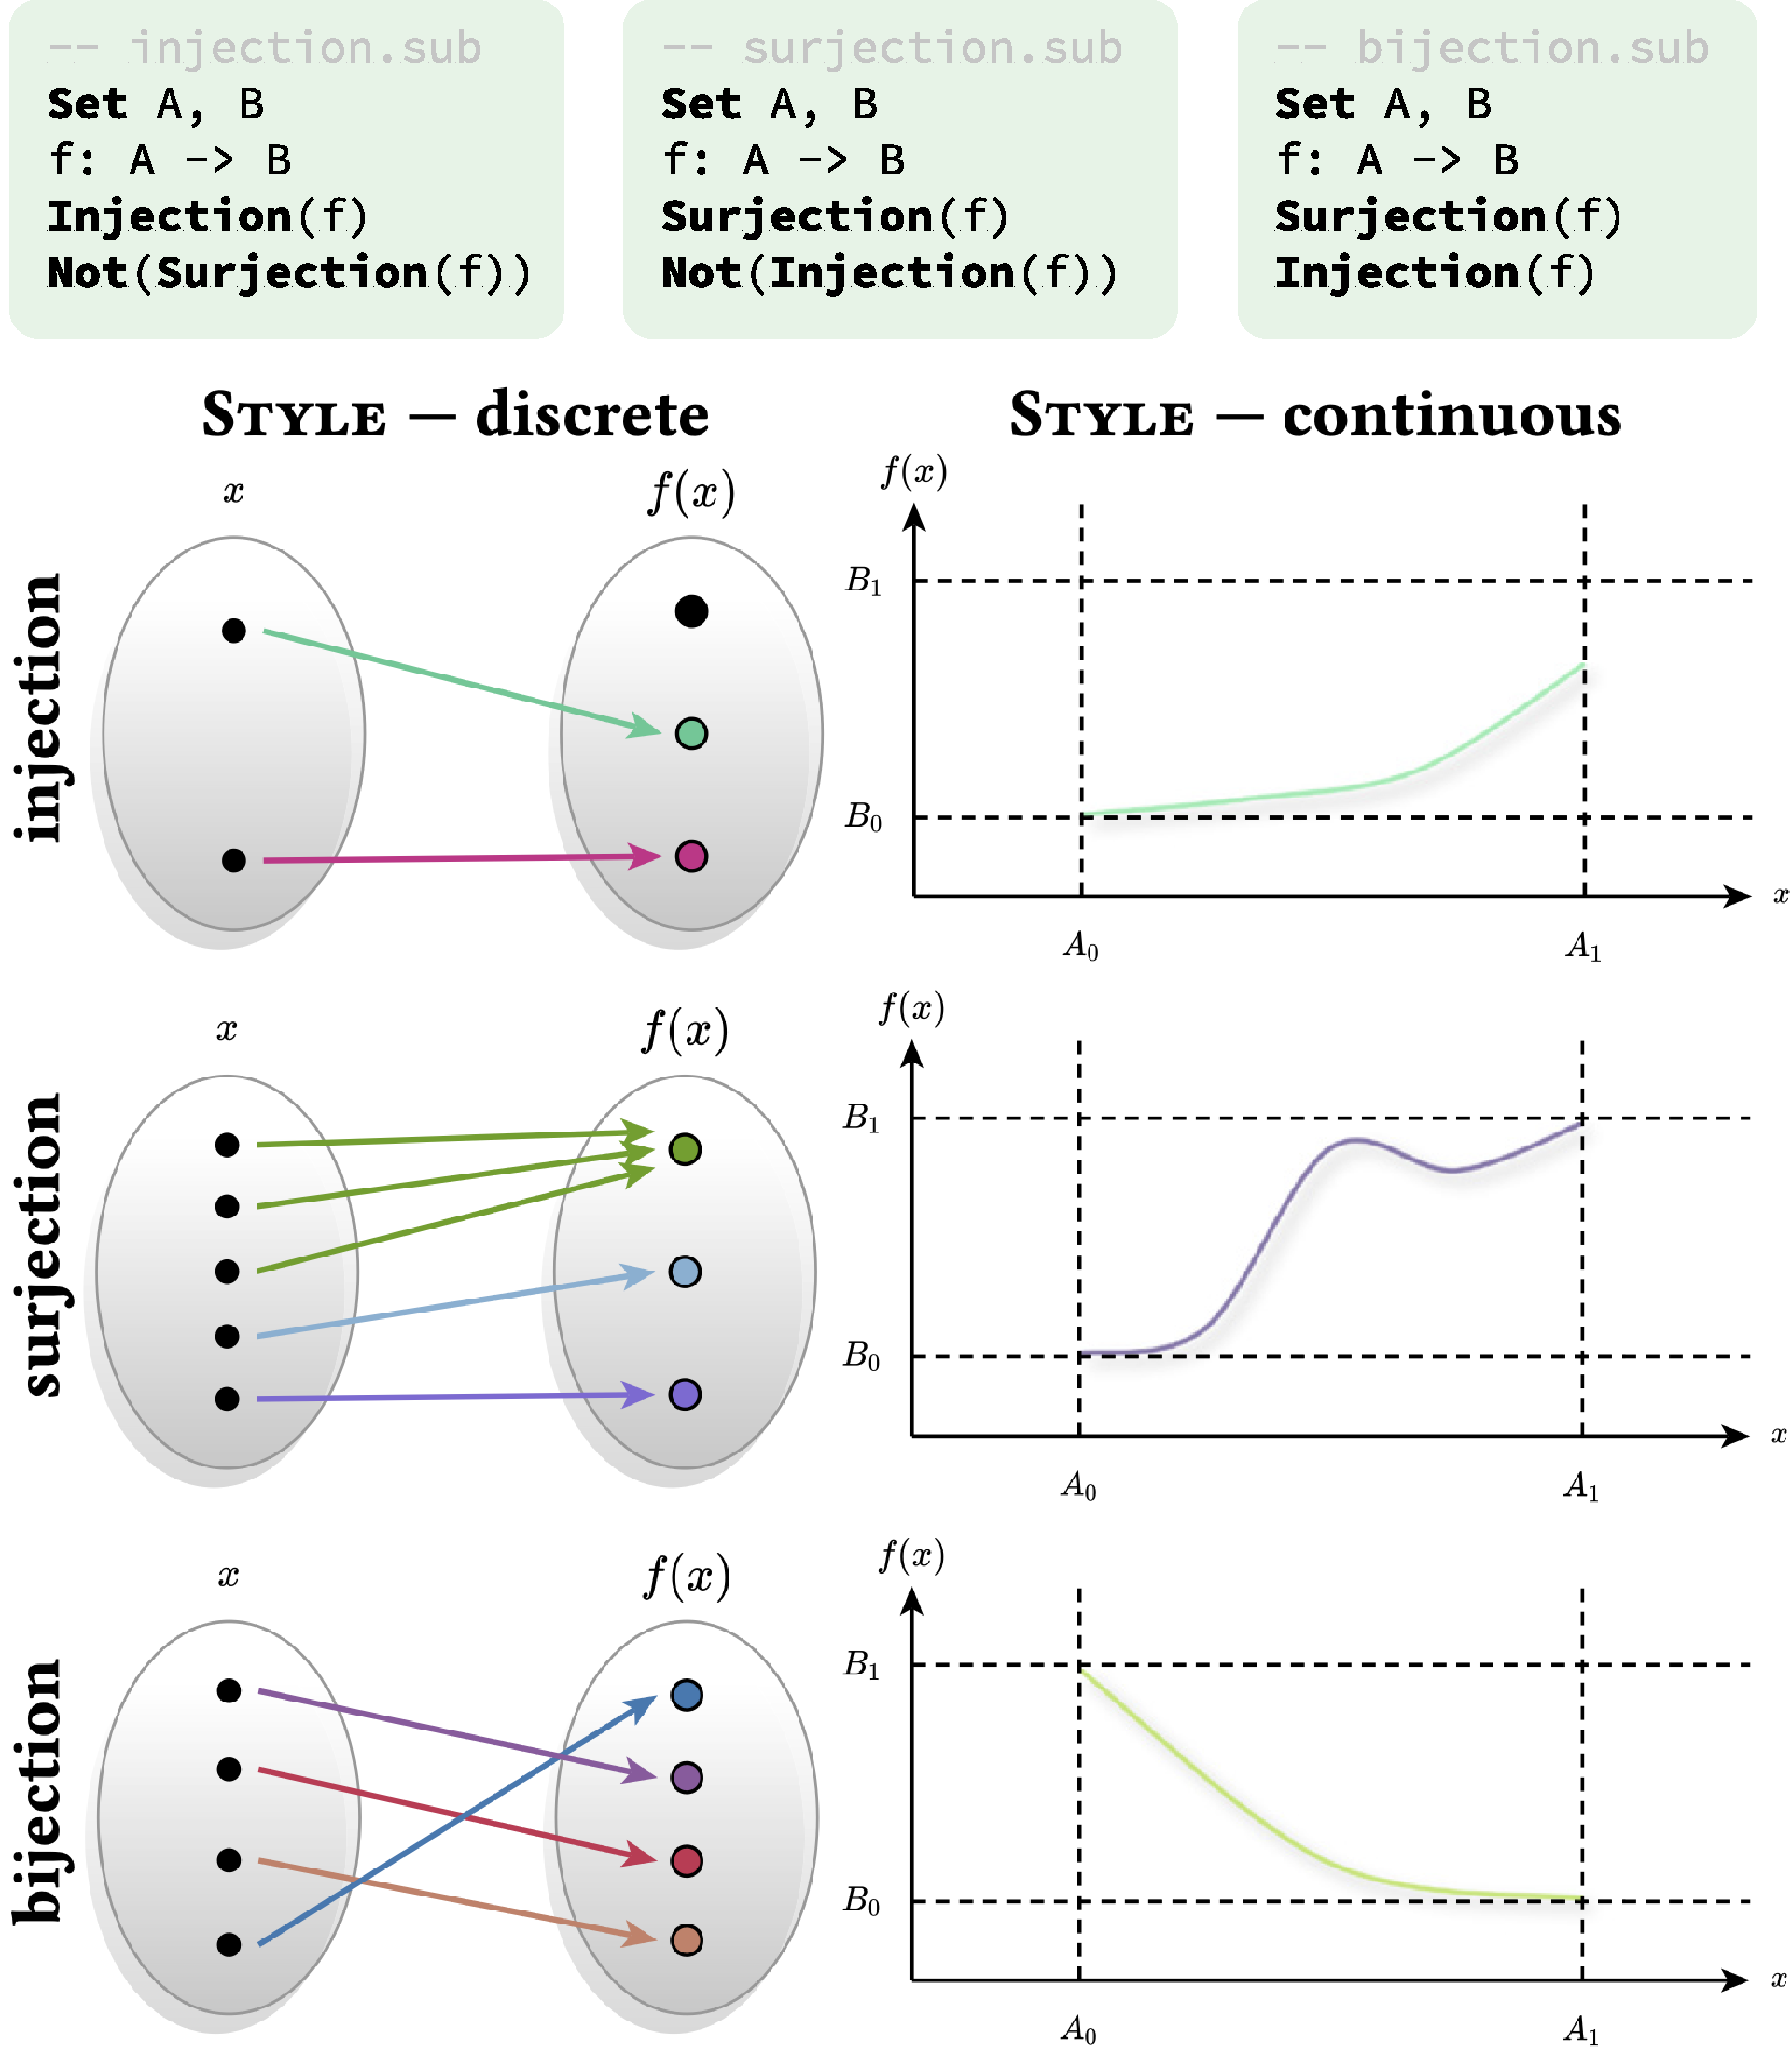
\includegraphics[width=\textwidth]{assets/chapter-2/injection-surjection-bijection.pdf}
% \end{minipage}
% \end{figure}
    
% With the extensible design, \Penrose can automatically generate diagrams from many different domains using familiar syntax. \Penrose-generated geometry, real analysis, ray-tracing, set theory, and algebra are shown below.

% \vspace{10pt}
% 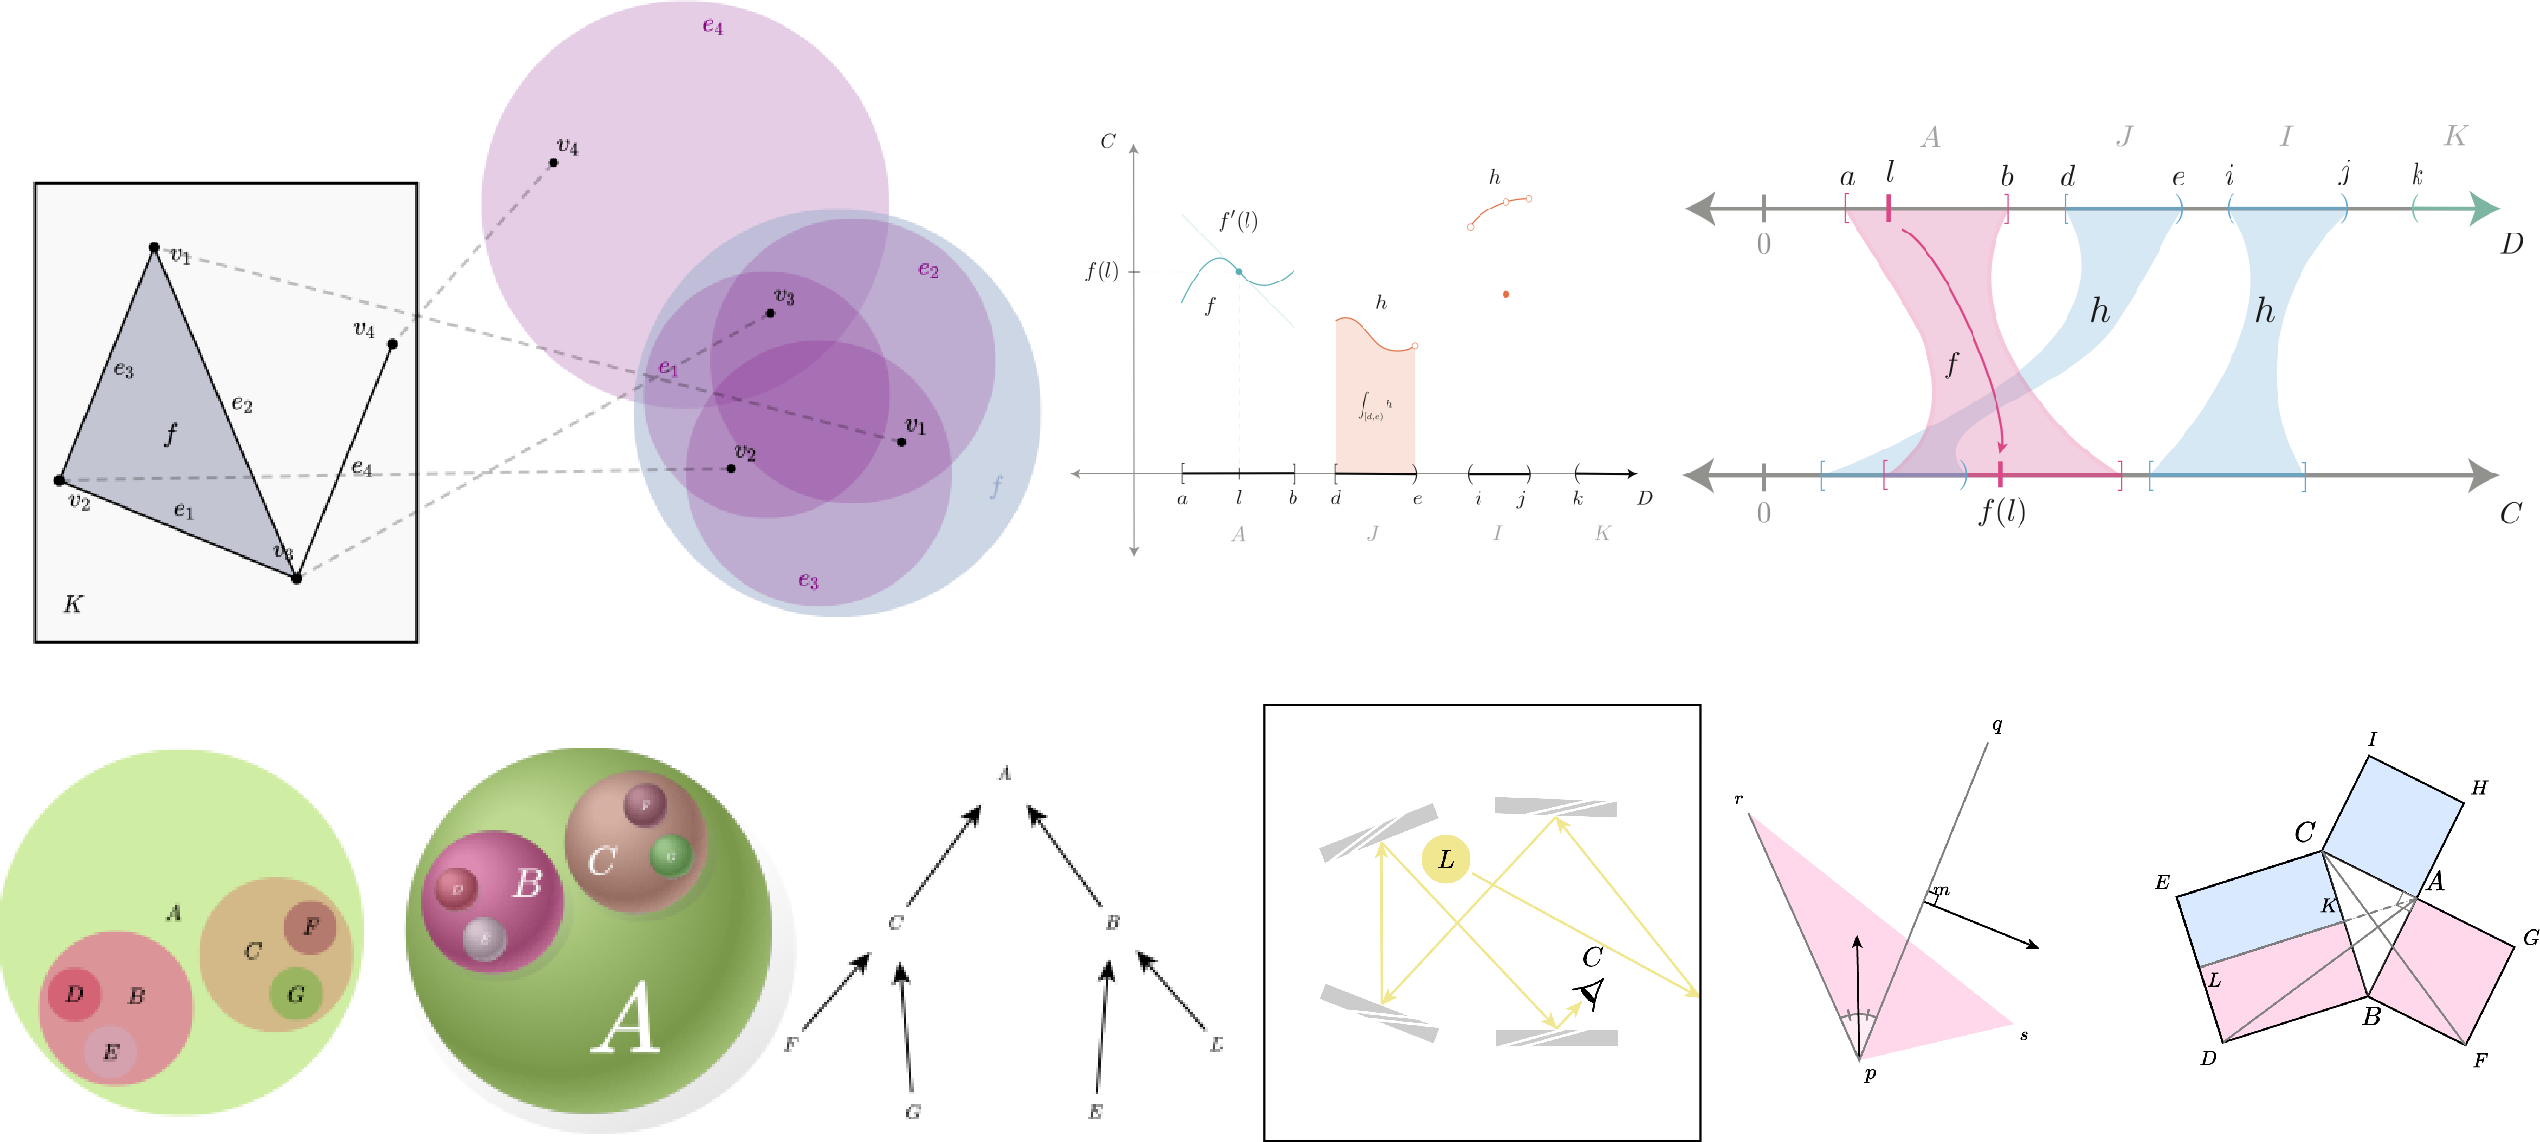
\includegraphics[width=0.95\linewidth]{assets/chapter-2/gallery.pdf}

\chapter[\Edgeworth: Diagrammatic Problem Authoring at Scale]{\Edgeworth: Diagrammatic Problem Authoring at Scale\footnote{This chapter is adapted from Sections 1 to 5 of ``\citefield{ni_edgeworth_2024}{title}''~\cite{ni_edgeworth_2024}.}}
\label{chp:edgeworth}

\begin{figure}[h]
    \centering
    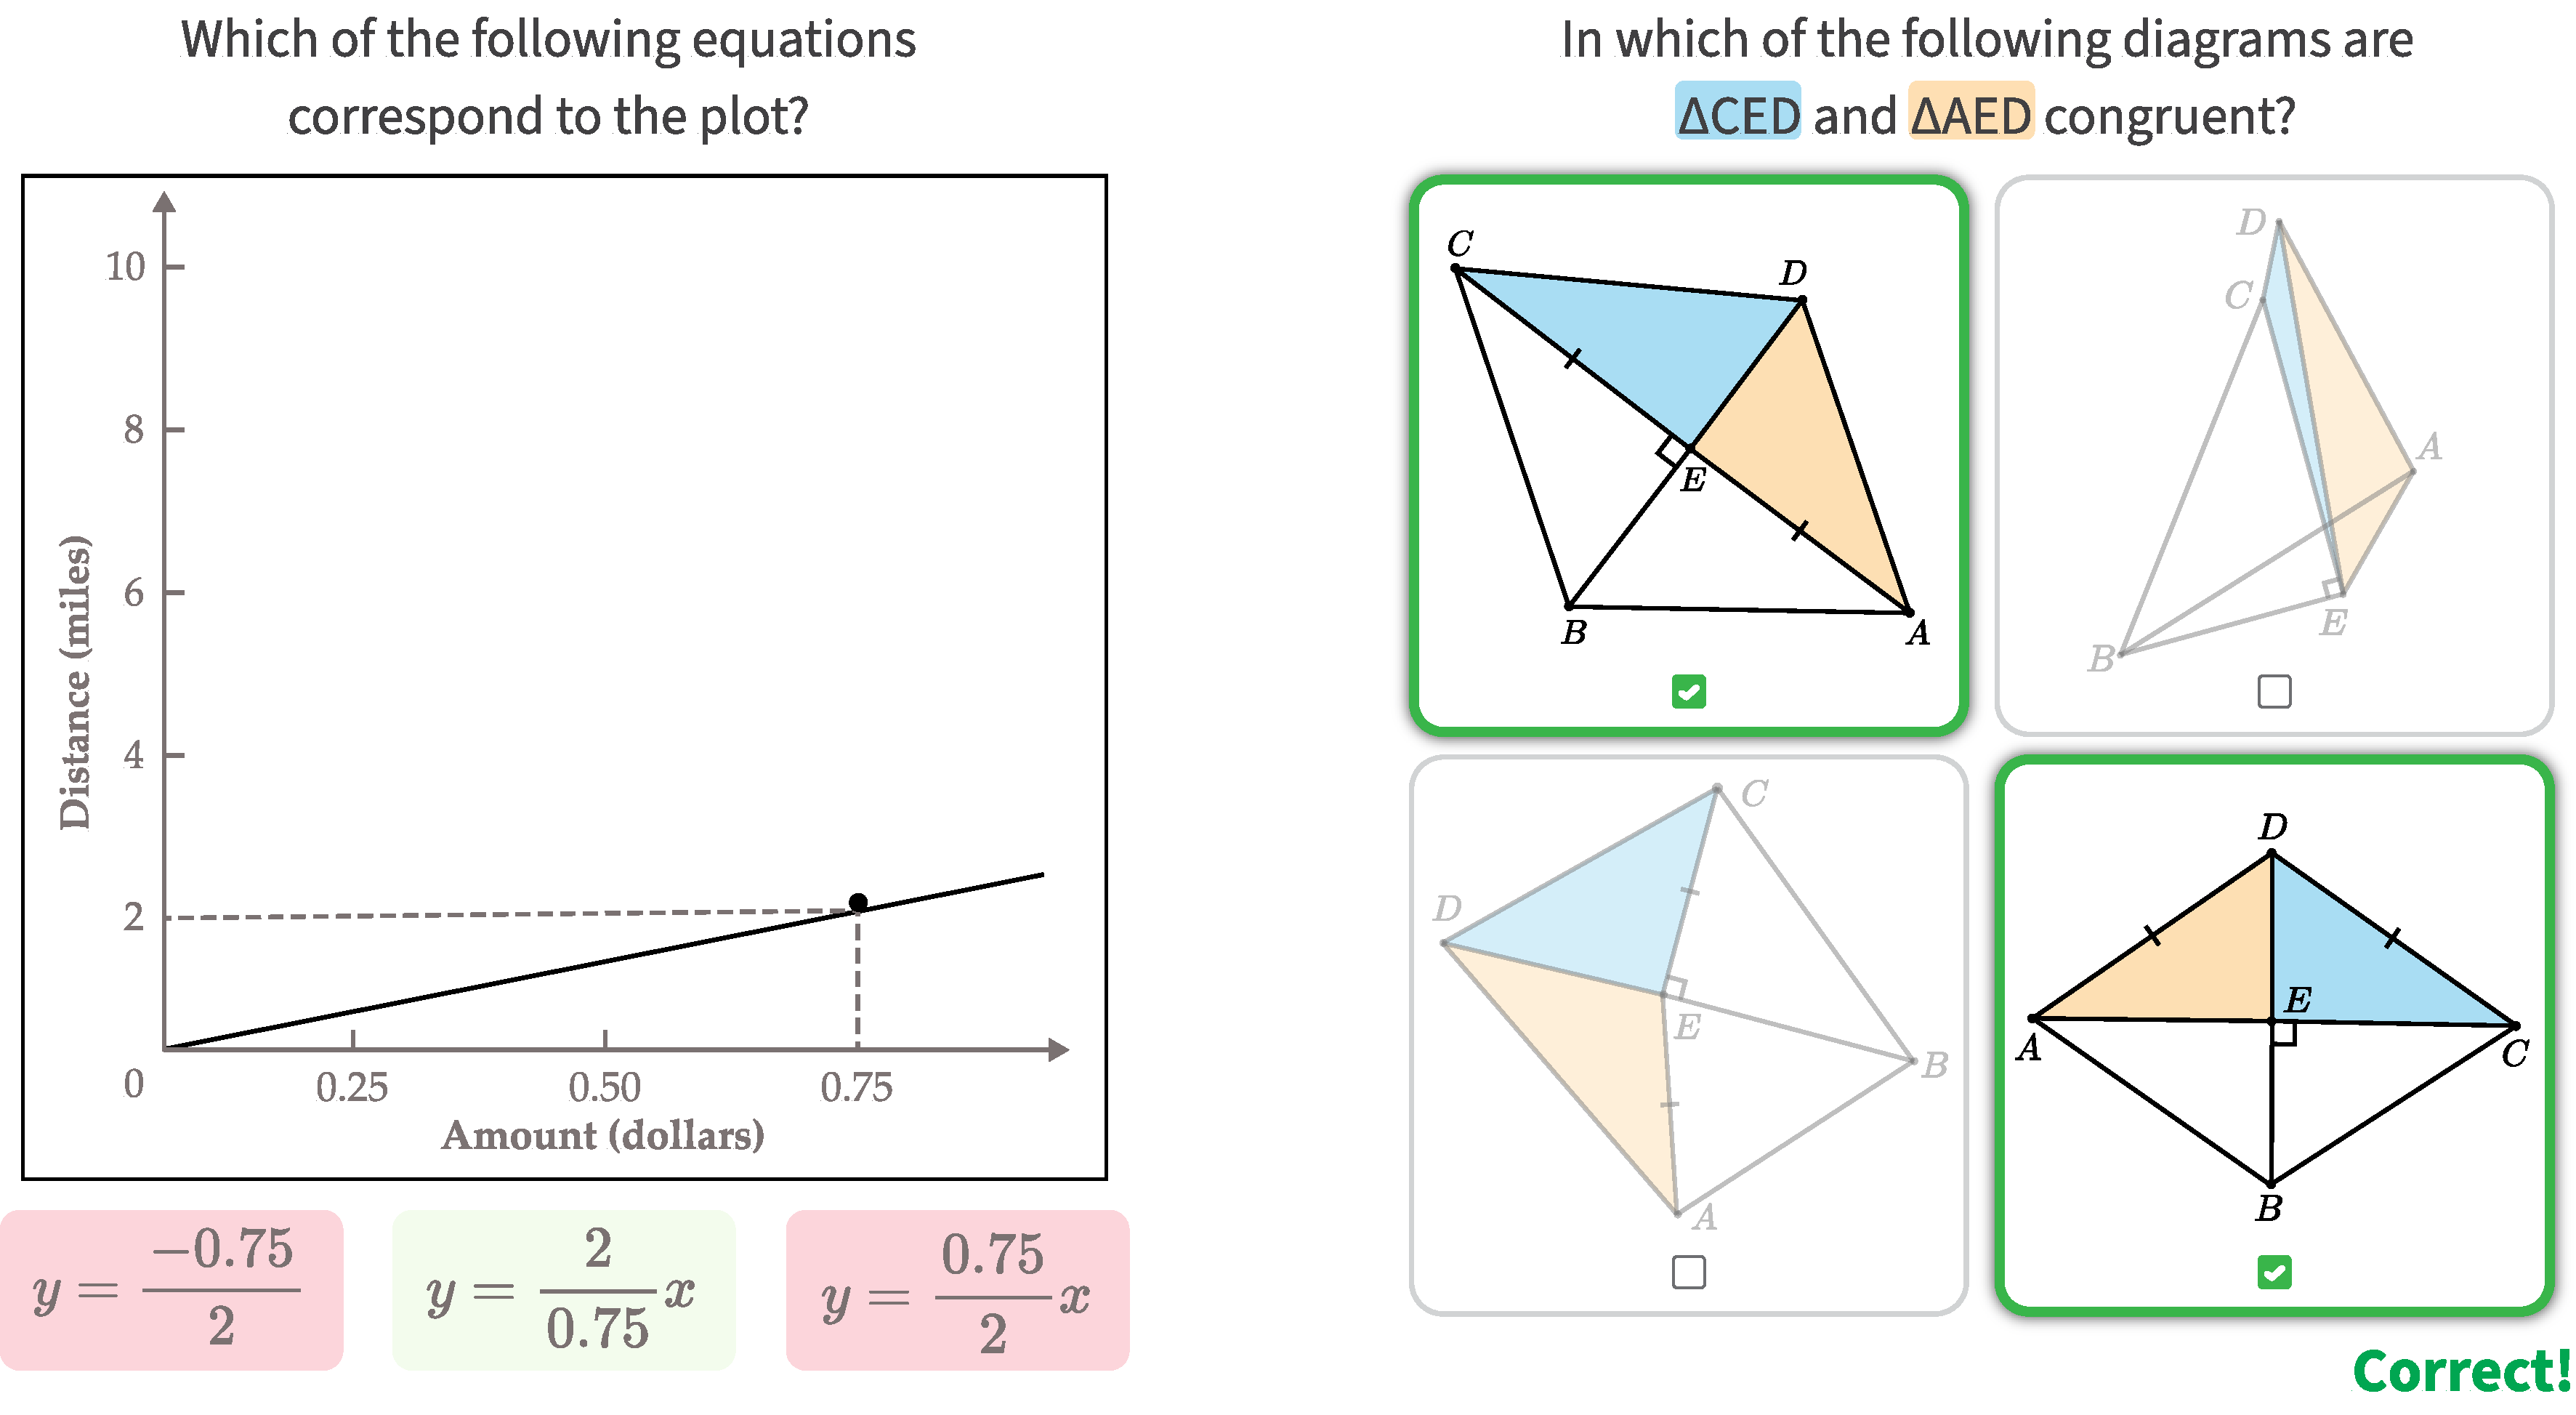
\includegraphics[width=0.88\linewidth]{assets/edgeworth/translation-problem.pdf}
    \caption{\textbf{left}: a translation problem that helps students discern the structure of linear equations (adapted from~\cite{perceptualLearning}). \textbf{right}: an \Edgeworth generated problem that trains student to recognize diagram configurations~\cite{Koedinger1990a} for triangle congruence.}
    \label{fig:translation-problem}
\end{figure}

\vspace{10pt}

\begin{figure}
    \centering
    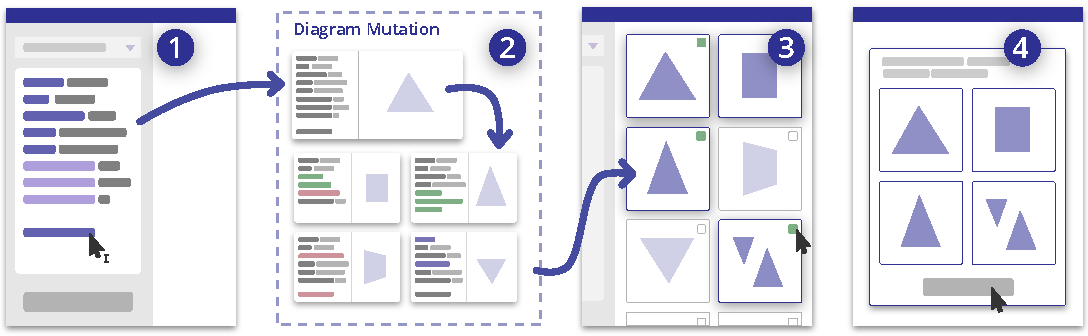
\includegraphics[width=\linewidth]{assets/edgeworth/edgeworth-teaser.pdf}
    \caption{\Edgeworth is a diagrammatic problem authoring tool that automatically generates diagram variations from a single diagram: \textmd{the author creates an example diagram~(\uilabel{1}), then \Edgeworth generates a myriad of diagram variations~(\uilabel{2}), from which the author selects diagrams~(\uilabel{3}) to form a diagrammatic multiple choice problem~(\uilabel{4}).}}
    \label{fig:teaser}
\end{figure}

\section{Introduction}

Effective use of visual representations requires a certain level of \emph{representational fluency} that's achievable through deliberate practice and repetition~\cite{metarepresentation, representationalFluency}. Recognizing how words, symbols, and diagrams relate to each other is an important first step of achieving fluency. Prior work has shown that these contrasting cases, \ie, discrimination and mapping, among representations significantly improve students' ability to translate among representations~\cite{perceptualLearning}.

To train students' representational fluency, educators often create problem sets that involve numerous contrasting cases of a particular visual representation. For instance, \cref{fig:translation-problem}~shows two examples of \emph{translation problems}, where the problem asks students to determine diagrammatic \emph{examples} and \emph{counterexamples} of a textual description and vice versa. Importantly, these examples and counterexamples have varying degrees of differences from the given diagram or text, and carefully picking examples on this spectrum has a big impact on learning~\cite{samenessAndDifference}.

Traditionally, educators author visual practice by drawing diagrams by hand. In formative interviews (\cref{sec:edgeworth-formative}), educators reported the vital role of visual practice in their instruction, but noted the tedium of authoring due to tool limitations, leading to fewer diagrams used than desired. Manual authoring can hardly keep up with the growth of STEM learners and demand for more visual practice.

As a first step towards scaling up visual practice authoring, we built \Edgeworth, a diagrammatic problem generator. \Edgeworth generates \emph{translation problems}, an effective type of visual practice~\cite{perceptualLearning} that ask students to determine diagrammatic \emph{examples} and \emph{counterexamples} of a textual/symbolic description (\cref{fig:translation-problem}). To help authors get the most out of one diagram, \Edgeworth contributes a ``build once, generate many'' authoring paradigm: Instead of manually editing diagrams to get variations, the author creates a single diagram and \Edgeworth automatically generates diagram variations (\cref{fig:teaser}\uilabel{1}\uilabel{2}). The interaction design of \Edgeworth allows the author to visually select diagram variations to rapidly form translation problems (\cref{fig:teaser}\uilabel{3}\uilabel{4}). Given the diversity of instructional contexts in STEM, we designed \Edgeworth to be domain-agnostic: it uses a generic program mutation technique~(\cref{sec:edgeworth-mutation}) to change the author-provided diagram to produce variations. 

In this chapter, we discuss formative interviews that drove the design of \Edgeworth{} and then walk through the technical implementation of \Edgeworth.

\section{Formative interview}

\label{sec:edgeworth-formative}

We conducted semi-structured interviews with 6 educators to understand how they author, use, and maintain diagrammatic problems. We recruited participants based on their background in education and usage of diagrams in their work. Selected participants work as secondary school teachers, university professors, teaching assistants, and competitive math coaches. All participants (P1--6) indicated that they have experience creating instructional material, authoring problems, and/or developing online courses that include visual content. Example interview questions include what roles diagrams play in the participant's educational materials, how students interact with diagrams, and how diagrams are authored and maintained. 
% The full interview protocol is included in supporting files.

Participants reported the usage of diagrams to build conceptual understanding and emphasized the need for deliberate practice to acquire representational fluency. Traditional educational materials, especially in higher education, tend to emphasize \quotei{procedures, memorization, and symbolic manipulation} (P6).  Similarly, teachers such as P1 suffer from \quotei{the curse of knowledge} of teaching visual fluency: teachers tend to \quotei{under-train} students and they struggle to use visuals for problem-solving.  As a result, students often become \quotei{symbolically good} and do not develop \quotei{good conceptual understanding} (P3). Visuals like diagrams and graphs provide alternative representations that help students \quotei{develop intuition} (P3) and \quotei{become better problem-solvers} (P4). To improve their instruction, all of our participants (P1--6) attempt to incorporate more diagrams in their instructional materials. Some also ask students to draw, annotate, and explain diagrams (P1, P2, P6). P2 encourages students to learn \quotei{multiple representations} and makes diagrams central to their math and programming curricula. When students practice with diagrams, teachers also gain richer feedback on students' level of understanding, and \quotei{learned more from this [student-drawn diagram] than 10 similar problems without the pictures} (P6).

While the benefits of and need for diagrammatic practice are clear, participants reported that tool limitations led to manual and repetitive authoring experience. Because participants typically create many problems and iterate on their content often, they face a trade-off when authoring visual content: more visuals are beneficial for learning but are time-consuming to create and modify. When authoring practice problems, P1 struggled to \quotei{create simple shapes by myself} and always ended up \quotei{copy-pasting and searching online} repeatedly. Similarly, P6 reported that they \quotei{get online images for pre-made resources, but whenever I want something a little custom, it’ll take a lot of time.} To streamline the visual authoring process, P2 and P5 developed custom pipelines for authoring problem sets and quizzes using existing programming tools. Like the problems described by prior research on diagramming tool usability~\cite{naturalDiagramming}, these tools often lack support for \quotei{high-level tweaking of my diagrams} (P2) and \quotei{are a pain to use because the language is not semantic and hard to use for non-programmers} (P5). Participants showed us many examples of tedious changes necessary to create diagram variations.

From the results, we derived the following design requirements for tool design to address participants' needs:

\begin{enumerate}[label=\textbf{D\arabic*}]
    \item\label{req:fluency} Address the need for practicing representational fluency
    \item\label{req:variation} Simplify the workflow for generating diagram variations
    \item\label{req:layout} Obviate the need to attend to low-level diagramming details
\end{enumerate}



\section{System Design of \Edgeworth}
\label{sec:edgeworth-system-design}


\Edgeworth realizes the design goals from \cref{sec:edgeworth-formative} by: 1) providing a domain-agnostic workflow for rapidly authoring diagrammatic practice problems (\ref{req:fluency}), 2) automatically suggesting numerous diagram variations of a single example diagram and allowing the author to visually select from the variations (\ref{req:variation}), and 3) fully automating the layout for all diagram variations (\ref{req:layout}). \cref{fig:edgeworth-interface} walks through the user interface of \Edgeworth, a simple and clean design that encapsulates the ideas above.

In \cref{sec:edgeworth-workflow}, we demonstrate the workflow of \Edgeworth by showing how to author an example diagrammatic problem in Euclidean geometry. We then describe \Edgeworth's approach to diagram layout in \cref{sec:edgeworth-layout} and how it generates diagram variation in \cref{sec:edgeworth-mutation}. 

% Finally, we discuss the limitations of the current implementation in \cref{sec:limitations}.

\begin{sidewaysfigure}
    \centering
    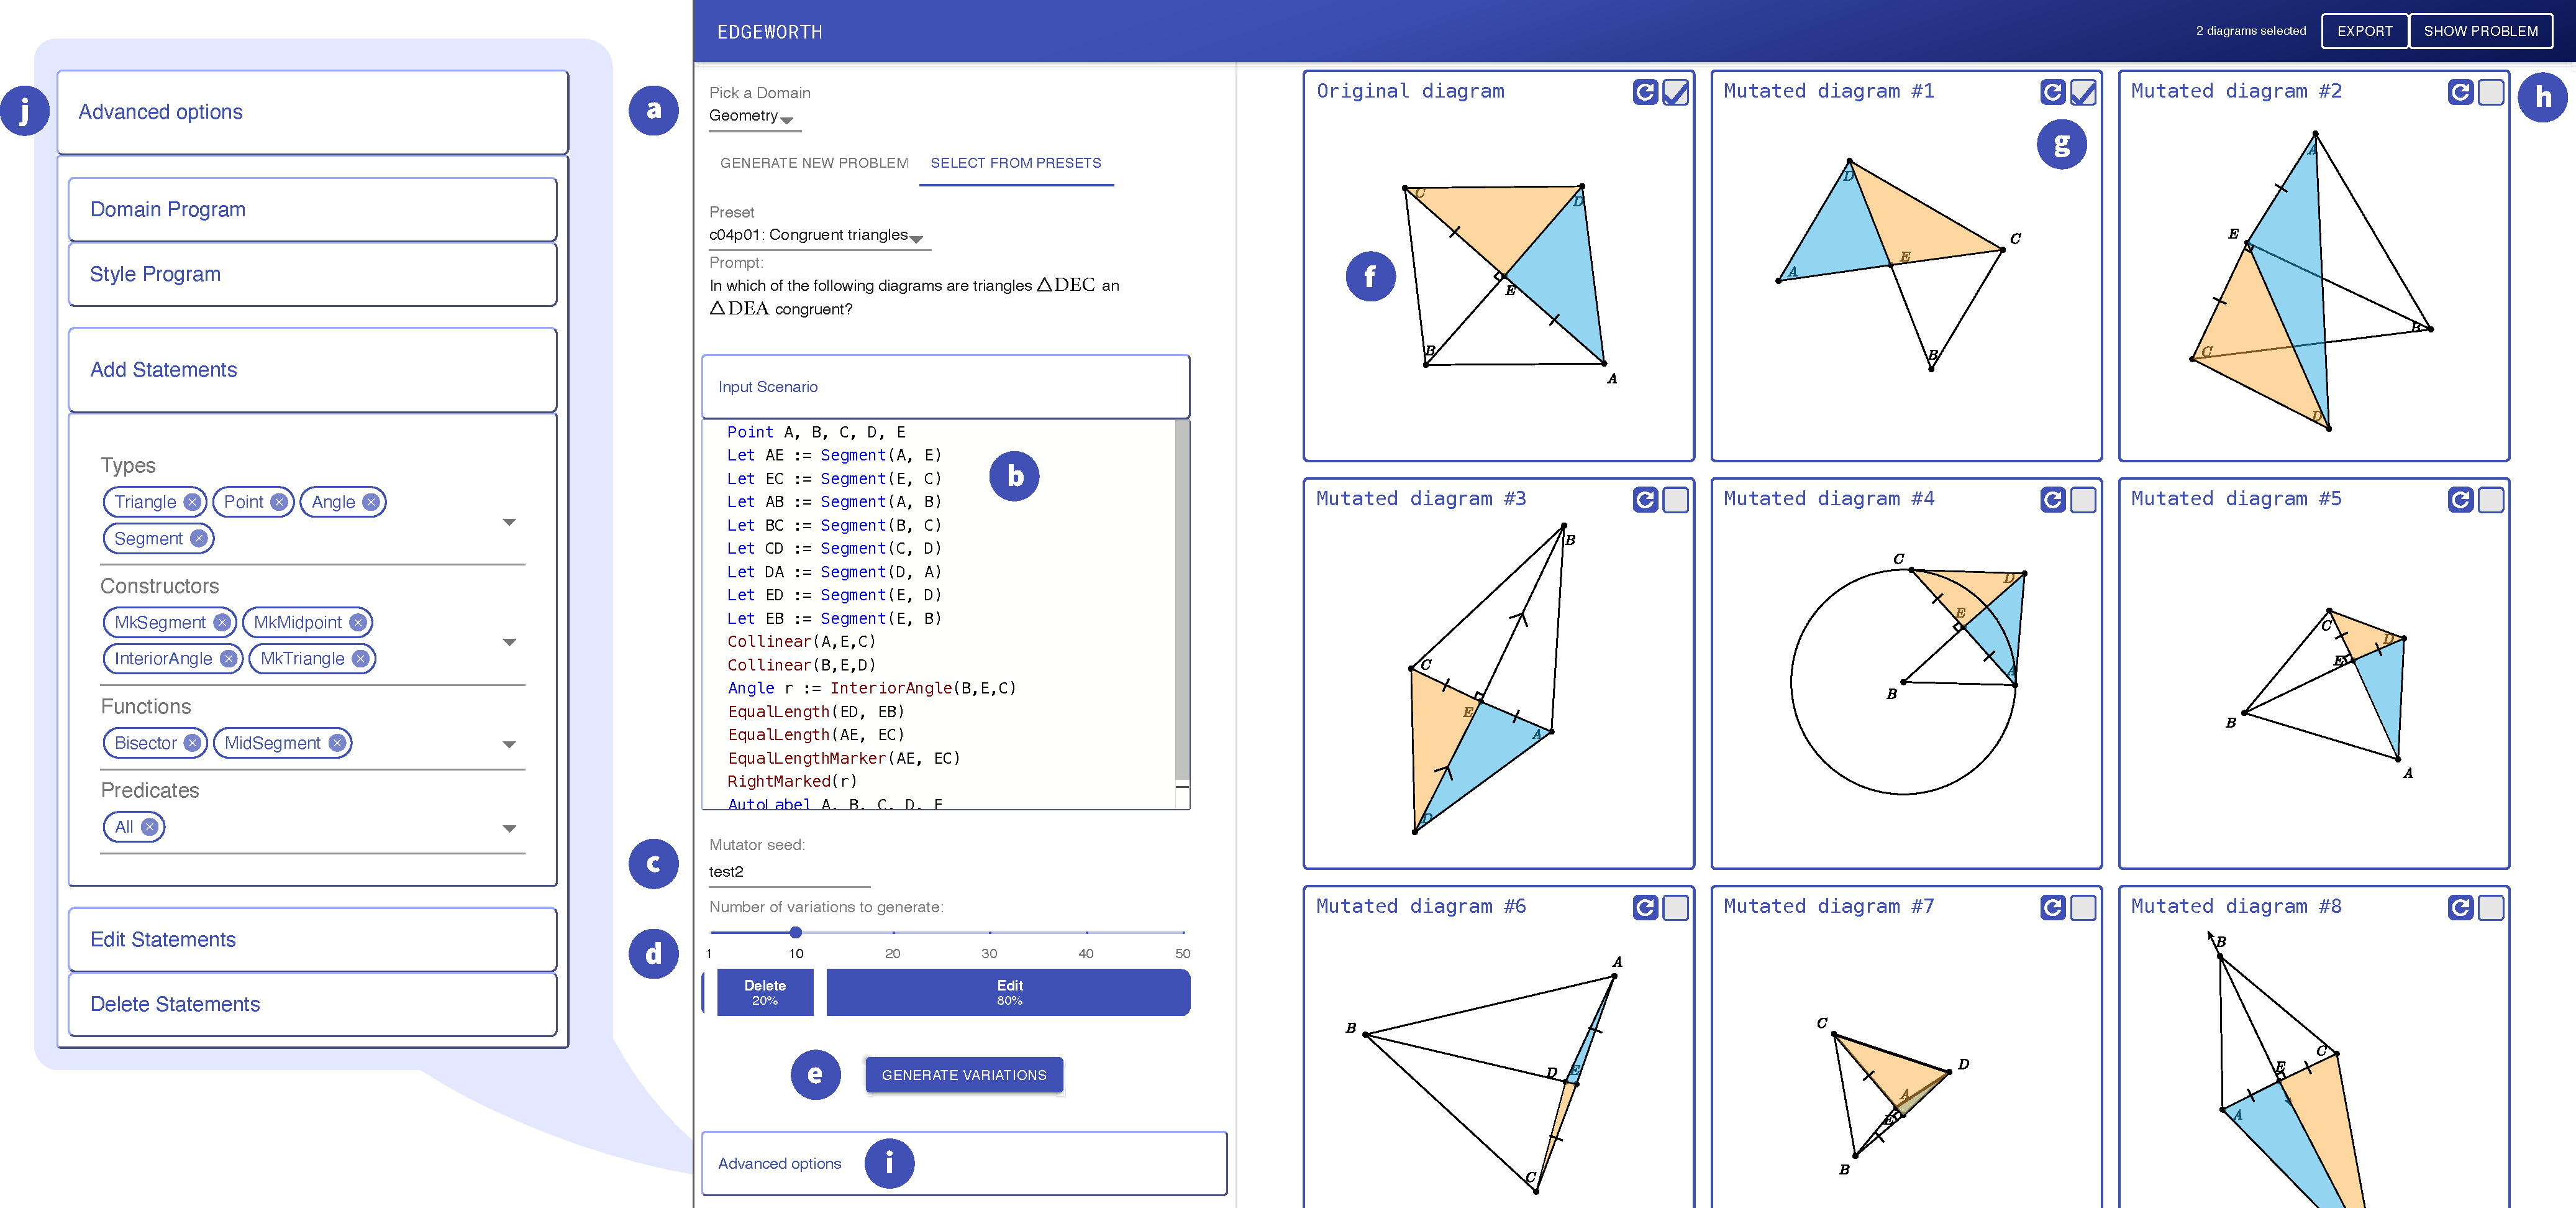
\includegraphics[width=\linewidth]{assets/edgeworth/edgeworth-ui-new.pdf}
    \caption{\textbf{The user interface of \Edgeworth.} \textmd{The author first provides a textual prompt~(\uilabel{a}) as an input scenario in \Substance notation~(\uilabel{b}). Then, clicking ``Generate Variations''~(\uilabel{e}) generates the specified number of diagram variations~(\uilabel{d}) at random based on a string seed and weights on Add, Delete, or Edit mutations~(\uilabel{c}). In the diagram panel, the top-left diagram~(\uilabel{f}) corresponds to the input scenario and the rest are diagram variations generated by \Edgeworth. The author can visually select diagrams~(\uilabel{g}) to assemble a diagrammatic multiple-choice problem~(\uilabel{h}). If needed, the author can fine-tune the mutator using ``Advanced options'' (\uilabel{i}\uilabel{j}}).}
    \label{fig:edgeworth-interface}
\end{sidewaysfigure}

\subsection{Author Workflow}
\label{sec:edgeworth-workflow}

In this section, we use an example from high school geometry to demonstrate the process of creating a problem in \Edgeworth, the user interface of which is annotated in \cref{fig:edgeworth-interface}. 

\subsubsection{Create an example diagram} 
\label{sec:create-scenario}

The author wants to write a problem about triangle congruence to assess students' understanding of the \textit{Side-Angle-Side} (SAS) rule. They want to create a translation problem including one diagram where the SAS rule is satisfied and three others where it is not. The author first describes an example diagram (\cref{fig:edgeworth-interface}\uilabel{b}) where this rule is satisfied. They construct a scenario involving two triangles: $\triangle DEC$ and $\triangle DEA$ share one side $DE$ and have two equal sides $EC$ and $EA$. $\angle CEB$ indicates that $AC$ and $BD$ are perpendicular and therefore $\angle DEC = \angle DEA$. Therefore, $\triangle DEC$ and $\triangle DEA$ are congruent by the SAS rule. Given this description, \Edgeworth lays out the diagram automatically (\cref{fig:edgeworth-interface}\uilabel{f}). 

% \Edgeworth mutates this scenario to create variations that may or may not satisfy the SAS rule, and the author can select from these variations to create their translation problem. While \Edgeworth requires an example scenario, it does not require it to be correct or incorrect. The choice of this scenario is specific to the format of translation problems in this problem set. Constructing the example first guarantees that there will be at least one correct choice in the problem. If the author starts with an incorrect scenario, \Edgeworth may still mutate it to create a correct choice, but it is not guaranteed.

\subsubsection{Select from \Edgeworth-generated diagrams}
\label{sec:select-diagrams}

Now the author can use \Edgeworth to mutate the example diagram by clicking ``Generate Variations'' (\cref{fig:edgeworth-interface}\uilabel{e}). \Edgeworth performs mutations on the example scenario and generates a grid of diagram variations. The grid is designed to give the author an overview of the mutation results, and diagrams are prominent in each cell to facilitate faster visual selection. The top-left cell in the grid will always display the original example diagram (\cref{fig:edgeworth-interface}\uilabel{b}\uilabel{f}), and the rest correspond to mutation results.

By inspecting each diagram in the grid, the author can determine if it is a good fit for their translation problem. If so, they click the top-right checkbox (\cref{fig:edgeworth-interface}\uilabel{g}) to include the diagram in the problem.

\subsubsection{Preview and export the problem}
After the author picks a sufficient number of diagrams (4 in this case), they can preview the translation problem by clicking ``Show Problem'' (\cref{fig:edgeworth-interface}\uilabel{h}), which displays an interactive multiple-choice widget. If the author is satisfied, they can click ``Export'' to download the diagrams and metadata to use the problem in their context. \Edgeworth exports to Scalable Vector Graphics (SVG) images for static media, source programs for interactive use, and detailed mutation trace metadata for comprehensive analysis and reference purposes.

\subsection{Diagram Notation and Layout}
\label{sec:edgeworth-layout}

\Edgeworth is built on \Penrose~(\cref{chp:penrose}). Compared with alternatives, \Penrose offers two distinct advantages: (1) a high-level diagram notation that's easy for authoring and (2) an automatic layout engine. As discussed in \cref{chp:penrose}, a diagram in \Penrose consists of a textual description of the diagram content (\Substance) and a reusable layout stylesheet (\Style). As a reminder, \cref{fig:cocl2-example} shows the three kinds of \Substance statements: type statements (\eg \sub{Carbon c}) declare new objects; constructors (\sub{Bond b1 := SingleBond(c, cl1)}) create new objects from existing objects; and predicates (\sub{ZeroDots(c)}) indicate relations among objects. 

% \begin{wrapfigure}{r}{0.5\textwidth}
\begin{figure}[H]
    % \begin{center}
    \centering
    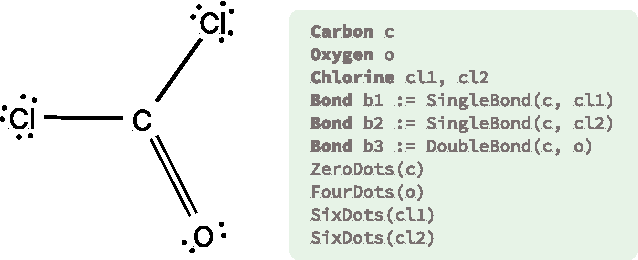
\includegraphics[width=.6\linewidth]{assets/edgeworth/cocl2-example.pdf}
    % \end{center}
    \caption{\textmd{Diagram and \Substance notation for the Lewis structure of phosgene (\ensuremath{\mathrm{COCl_2}}).}}
    \label{fig:cocl2-example}
\end{figure}

The current \Edgeworth implementation builds on \Penrose's geometry, chemistry, and graph \Style for diagram layout. Since the existing \Style stylesheets are primarily used to generate a few human-written examples, they lack coverage for variations of \Substance descriptions required by \Edgeworth. To this end, we improved \Style, diagram examples, and new standard library functions to \Penrose to accommodate \Edgeworth.

\Edgeworth is the first application of \Penrose that concurrently optimizes and renders a grid of multiple diagrams. Therefore, we have made significant updates to \Penrose to support \Edgeworth's use case. To make \Edgeworth a performant client-side web application for interactive use, we have migrated from Haskell to TypeScript and made various performance improvements to efficiently run tens of layout optimization jobs in a single session. Compared to the state of \Penrose at the publication of \citet{penrose}, the development of \Edgeworth has helped improve the performance of the system by 100$\times$.


\subsection{Program Mutation}
\label{sec:edgeworth-mutation}

% what is program mutation and why it's a good fit
\Edgeworth generates diagram variations by mutating the example diagram written in \Substance. 
% what the operators are
We purposely designed the system to include a small set of simple and type-safe mutation operations. Similar to generic tree-editing algorithms~\cite{gumtree}, \Edgeworth supports 3 kinds of mutation operators: \textbf{Add}, \textbf{Delete}, and \textbf{Edit}. \textbf{Add} appends a statement. \textbf{Delete} removes a statement and all other references to that statement. 

Since compilation errors in \Substance will not produce diagrams, \textbf{Edit} involves one of the type-safe patterns listed below. Each \textbf{Edit} pattern contains a \emph{guard} and an \emph{action}. The guard checks if the operator is applicable to the given \Substance statement, and the action performs the mutation. For instance, \textbf{Replace Arguments} is only applicable when the current context has existing variables of the desired type. 
\begin{itemize}[leftmargin=*]
    \item \textbf{Swap Arguments} reorders the arguments passed into a statement; \eg if \sub{A} and \sub{B} are \sub{Triangle}s:\\
            \sub{Similar(A, B)} $\rightarrow$ \sub{Similar(B, A)}
    \item \textbf{Replace Arguments} replaces the arguments passed into a statement with other arguments defined in scope; \eg if \sub{A, B, C, D} are \sub{Point}s:\\
            \sub{s := MkSegment(A, B)} 	$\rightarrow$ \sub{s := MkSegment(C, D)}
    \item \textbf{Replace Function} replaces a statement with a different statement that takes the same arguments; \eg if \sub{T} is a \sub{Triangle} and \sub{E} is an \sub{Angle}:\\
            \sub{Equilateral(T)} $\rightarrow$ \sub{Scalene(T)} \\
            \sub{Segment s := Bisector(E)} $\rightarrow$ \sub{RightAngleMarked(E)}
\end{itemize}

% one-col
\begin{algorithm}
\caption{The \Edgeworth mutation algorithm. }\label{alg:mutation}
\begin{algorithmic}[1]
\Function{Generate}{$p, \ell, h, a, d, e, A, D, E$}
\State $p' \gets p$
\State $n \gets \text{uniform random integer between $\ell$ and $h$}$\label{line:mutations}
\For{$i$ \textbf{from} $1$ \textbf{to} $n$}
    \State $x \gets \text{uniform random real between $0$ and $a + d + e$}$\label{line:kind}
    \If{$x < a$}
        \State $m \gets \textsc{RandomAdd}(A, p')$\label{line:add}
    \ElsIf{$x < a + d$}
        \State $m \gets \textsc{RandomDelete}(D, p')$\label{line:delete}
    \Else
        \State{$s \gets \text{uniform random element of $\textsc{Statements}(p')$}$}\label{line:statements}
        \State{$m \gets \textsc{RandomEdit}(E, s)$}\label{line:edit}
    \EndIf
    \State $p' \gets \textsc{Mutate}(p', m)$
\EndFor
\State \textbf{return} $p'$
\EndFunction
\end{algorithmic}
\end{algorithm}
% one-col

Algorithm~\ref{alg:mutation} shows how the \Edgeworth mutator works, at a high level. In addition to the input \Substance description $p$, \Edgeworth also takes a number of user-defined configuration parameters: (1) a number of variations to generate (the number of times \textsc{Generate} is called); (2) a range of mutation counts per variation (the input variables $\ell$ and $h$); (3) weights for \textbf{Add}, \textbf{Delete}, and \textbf{Edit} operations (the input variables $a$, $d$, and $e$ respectively); and (4) filter sets $A$, $D$, and $E$ which limit the set of mutations that the \textbf{Add}, \textbf{Delete}, and \textbf{Edit} operations can produce.

% how the mutator produces mutants
Given an example diagram, \Edgeworth performs several rounds of mutation generation. Each round results in a series of mutations that alter the input to produce a variation. The number of mutations (line~\ref{line:mutations}) is bounded by the configuration parameters.

To generate a single mutation, \Edgeworth makes a weighted choice (line~\ref{line:kind}) of the mutation kinds and enumerates all possible mutations for the chosen kind: \textbf{Add} enumerates all possible statements to add (line~\ref{line:add}); \textbf{Delete} randomly deletes an existing statement (line~\ref{line:delete}); \textbf{Edit} enumerates all possible edits for all statements (line~\ref{line:statements}) and picks one of them randomly (line~\ref{line:edit}). The randomness of \Edgeworth is controlled by a single random generator seed.

Users can specify filter sets under the ``Advanced options'' section of the UI, shown in \cref{fig:edgeworth-interface}\uilabel{i}\uilabel{j}. The filters default to ``All,'' which indicates that the mutator may change any statement in the example diagram. While this precise configuration may be useful, we ended up not using them in our evaluation (\cref{chp:edgeworth-eval}) and instead achieving our results using only \Edgeworth's simpler core set of configuration options, i.e., weights on mutation operators.

\section{Limitations}
\label{sec:limitations}

\subsection{Domains of instruction}
\label{sec:extension}

As shown in \cref{sec:edgeworth-mutation}, the design of the \Edgeworth mutator is domain-agnostic, as the mutation operators do not require any domain-specific knowledge to produce mutants. However, improving the layout domain expertise. Therefore, future \Edgeworth authors may not have the technical background or the time to invest in a new \Style program, which might prohibit them from using \Edgeworth if the domain is not well supported by the \Penrose ecosystem. In practice, as noted by \citet[Section~5]{penrose}, the effort to build \Penrose stylesheets for new domains is only necessary once per domain and not once per diagram or problem.

\subsection{Numerical and textual variations}

\Edgeworth cannot produce numerical and textual variations like traditional problem generators~\cite{CTAT, ASSISTment} do. It is, however, possible to build this functionality on top of \Edgeworth to produce further problem variations. 

% \cref{sec:problem-generation} further discusses this possibility in the context of existing template-based problem generation tools.

\subsection{Usability of UI components}

The design presented in \cref{sec:edgeworth-system-design} focuses on generating diagram variations and selecting diagram mutants to create problems. We use the \Substance language and \Penrose's textual interface without modification. Any limitations of \Substance and its UI are inherited by \Edgeworth. We use standard Material UI elements\footnote{\url{https://mui.com/}} to allow users to configure \Edgeworth (\eg a standard text box for changing diagram variations in \cref{fig:edgeworth-interface}\uilabel{c}). While these components might be usable as-is, they are not designed explicitly for the problem authoring workflow. 


\section{Translation Problem Dataset}
\label{sec:edgeworth-case-studies}

\begin{sidewaysfigure}
    \centering
    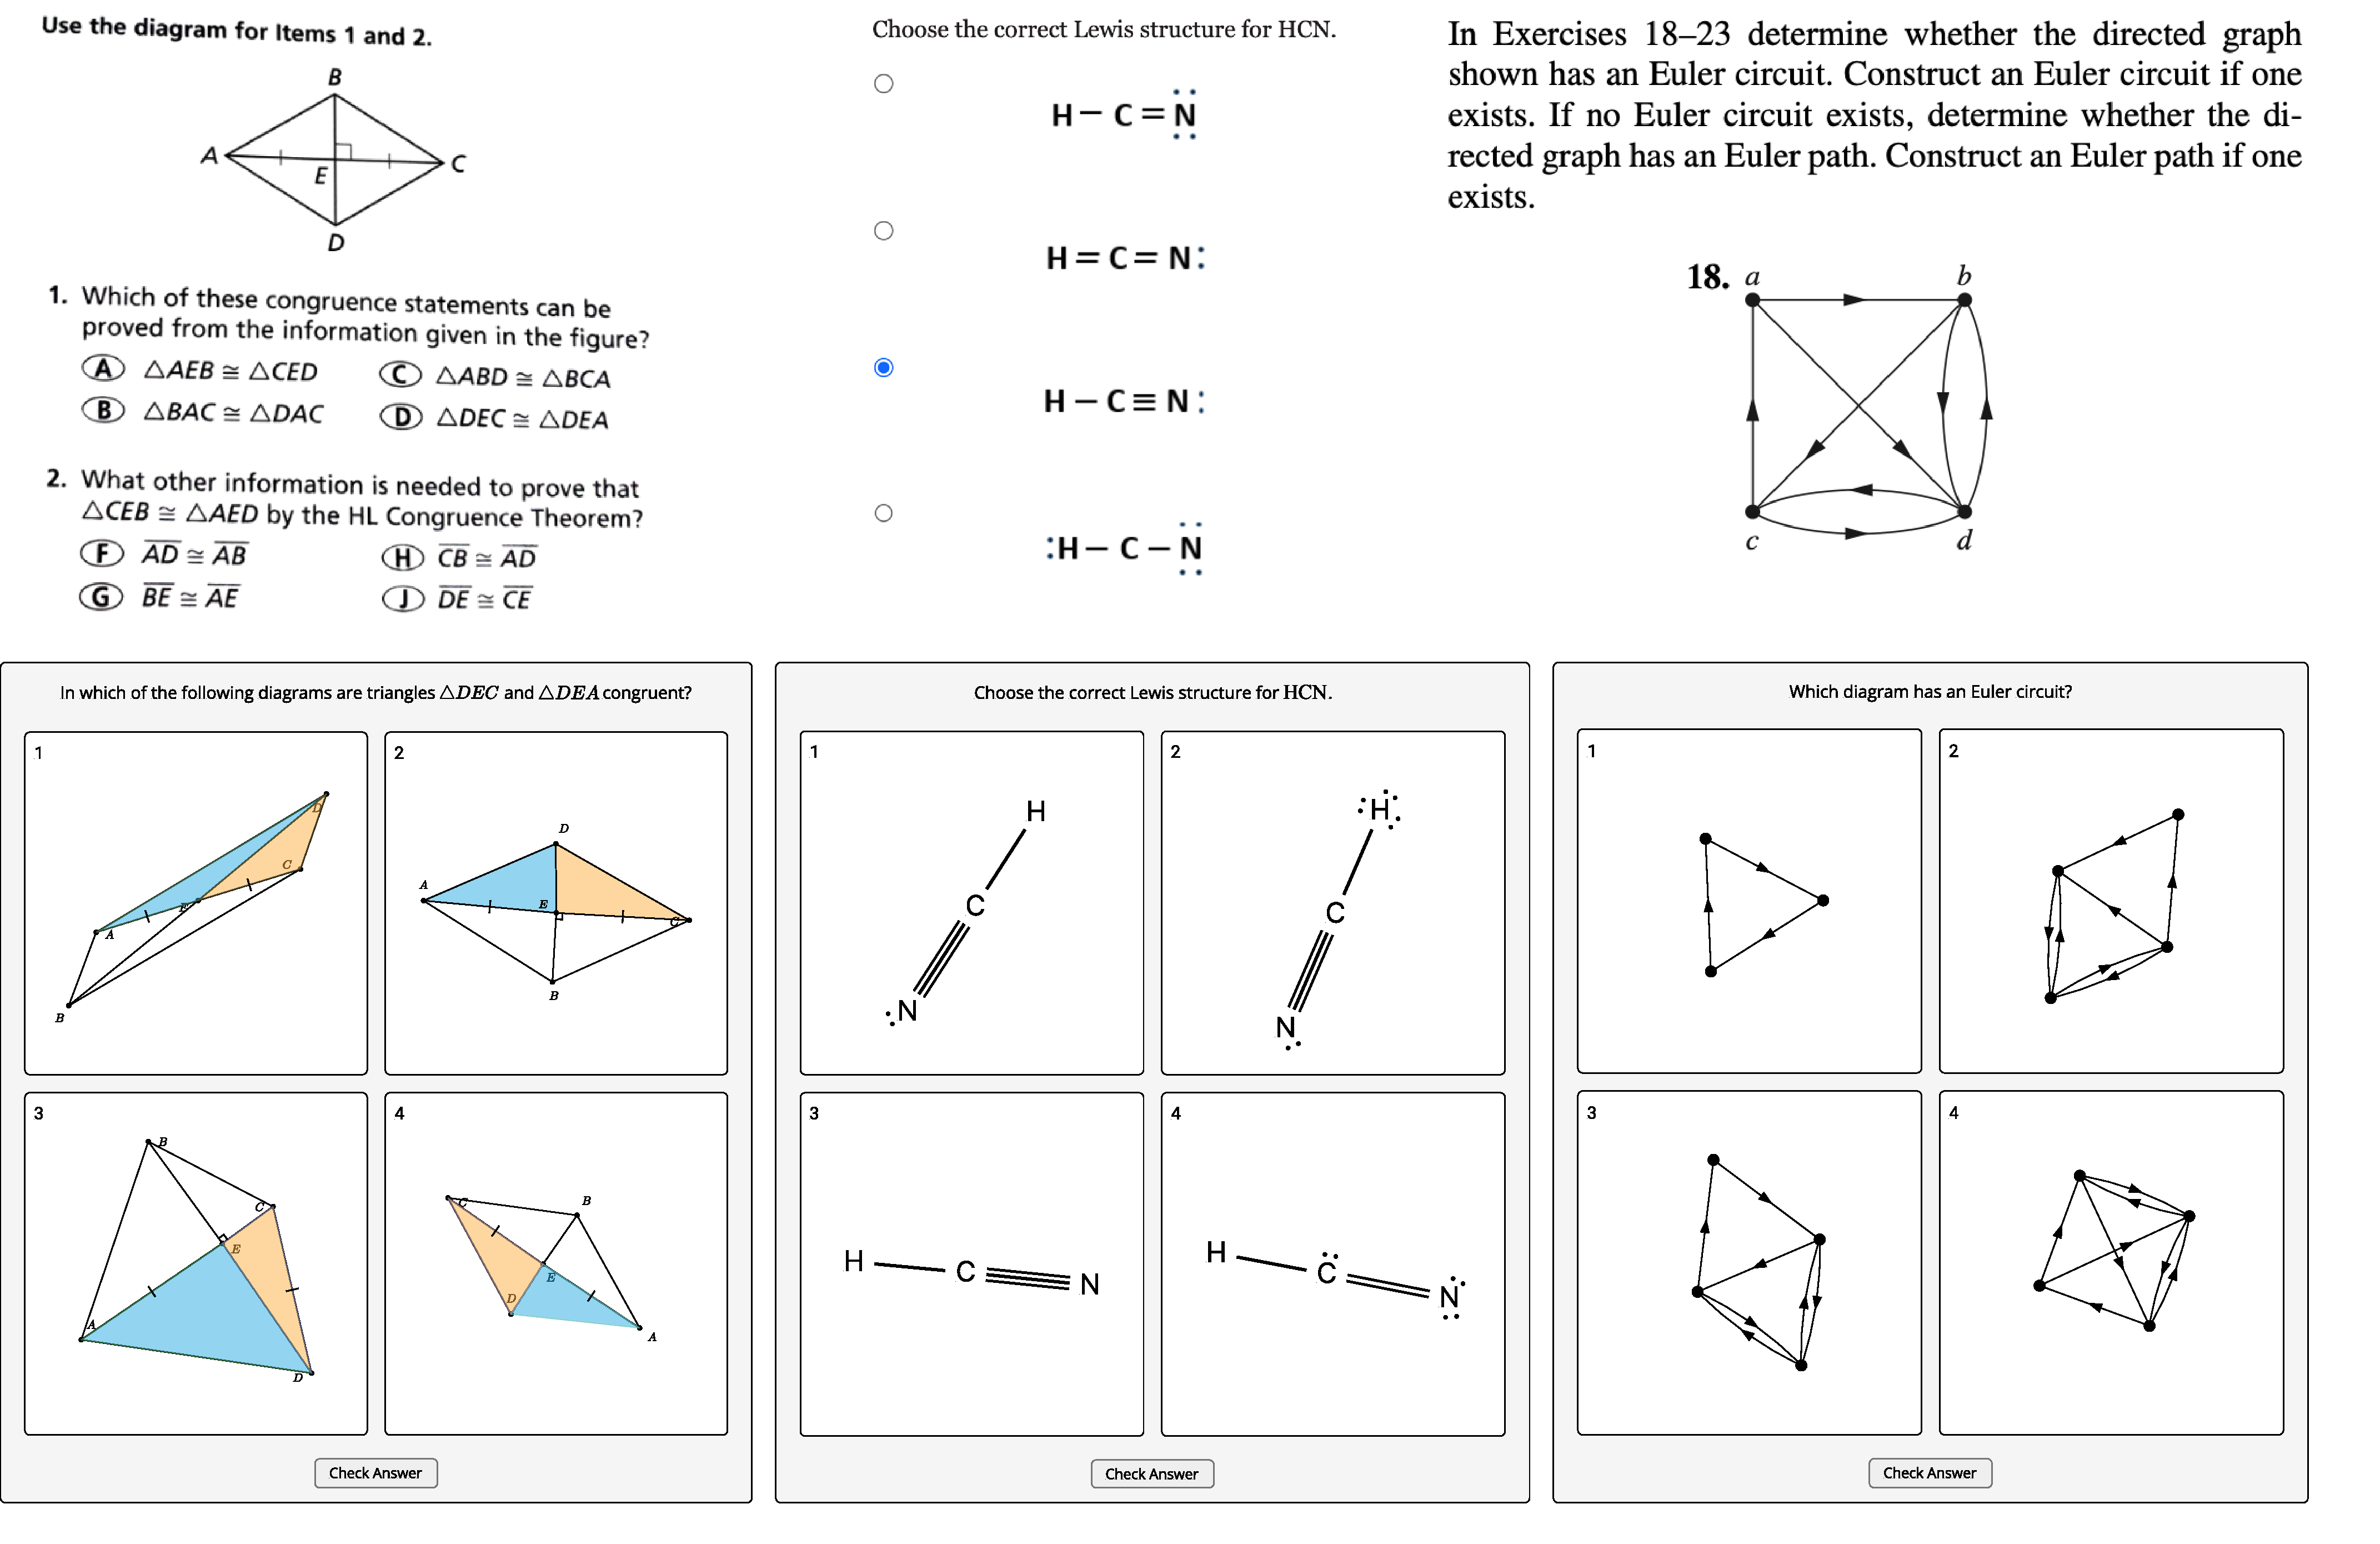
\includegraphics[width=\linewidth]{assets/edgeworth/problem-samples.pdf}
    \caption{We used \Edgeworth to recast real-world problems as diagrammatic translation problems. Left: \textmd{Determine if triangles are congruent.}  Middle: \textmd{Identify the correct Lewis structure for hydrogen cyanide.} Right: \textmd{Identify graphs with Euler circuits.}}
    \label{fig:edgeworth-problems}
\end{sidewaysfigure}

% motivation
\Edgeworth's mutation-based approach is domain-agnostic: it simply applies generic program mutations on any \Substance program. Through collecting a dataset of translation problems in Euclidean geometry, general chemistry, and discrete mathematics, we evaluate if this approach is expressive enough for different instructional contexts in STEM. The 3 domains are selected based on their ubiquity in STEM education and visual representations. All three domains have a wide audience in K-12 and higher education, making them rich sources for existing instructional materials. Each domain has canonical visual representations that are explicitly taught to students. Therefore, students can benefit from visual practice in these domains.

% procedure
We choose problems from existing textbooks or online courses and follow the procedure outlined in \cref{sec:edgeworth-workflow} to recast each problem. 

% All problems are included in supporting files. 

\subsection{Summary Statistics}
\label{sec:edgeworth-case-studies-summary}

We reproduced 31 problems in total. Since creating the example diagram (\cref{sec:create-scenario}) took the most time in this process, we report statistics on the example diagrams here. 

On average, \Edgeworth's diagram notation is compact and simple. The description for example diagrams are 14.7 lines of code ($\sigma = 4.57$) and 109.9 tokens ($\sigma = 48.6$). In contrast, the average SVG source of these same diagrams have 454.7 lines of code ($\sigma = 184.3$) and 1290.4 tokens ($\sigma = 650.4$). This indicates that \Edgeworth provides a concise and compact textual representation of diagrams across all three domains.

\subsection{Euclidean Geometry}
\label{sec:edgeworth-geometry}

% one-col 
\begin{figure}[h]
    \centering
    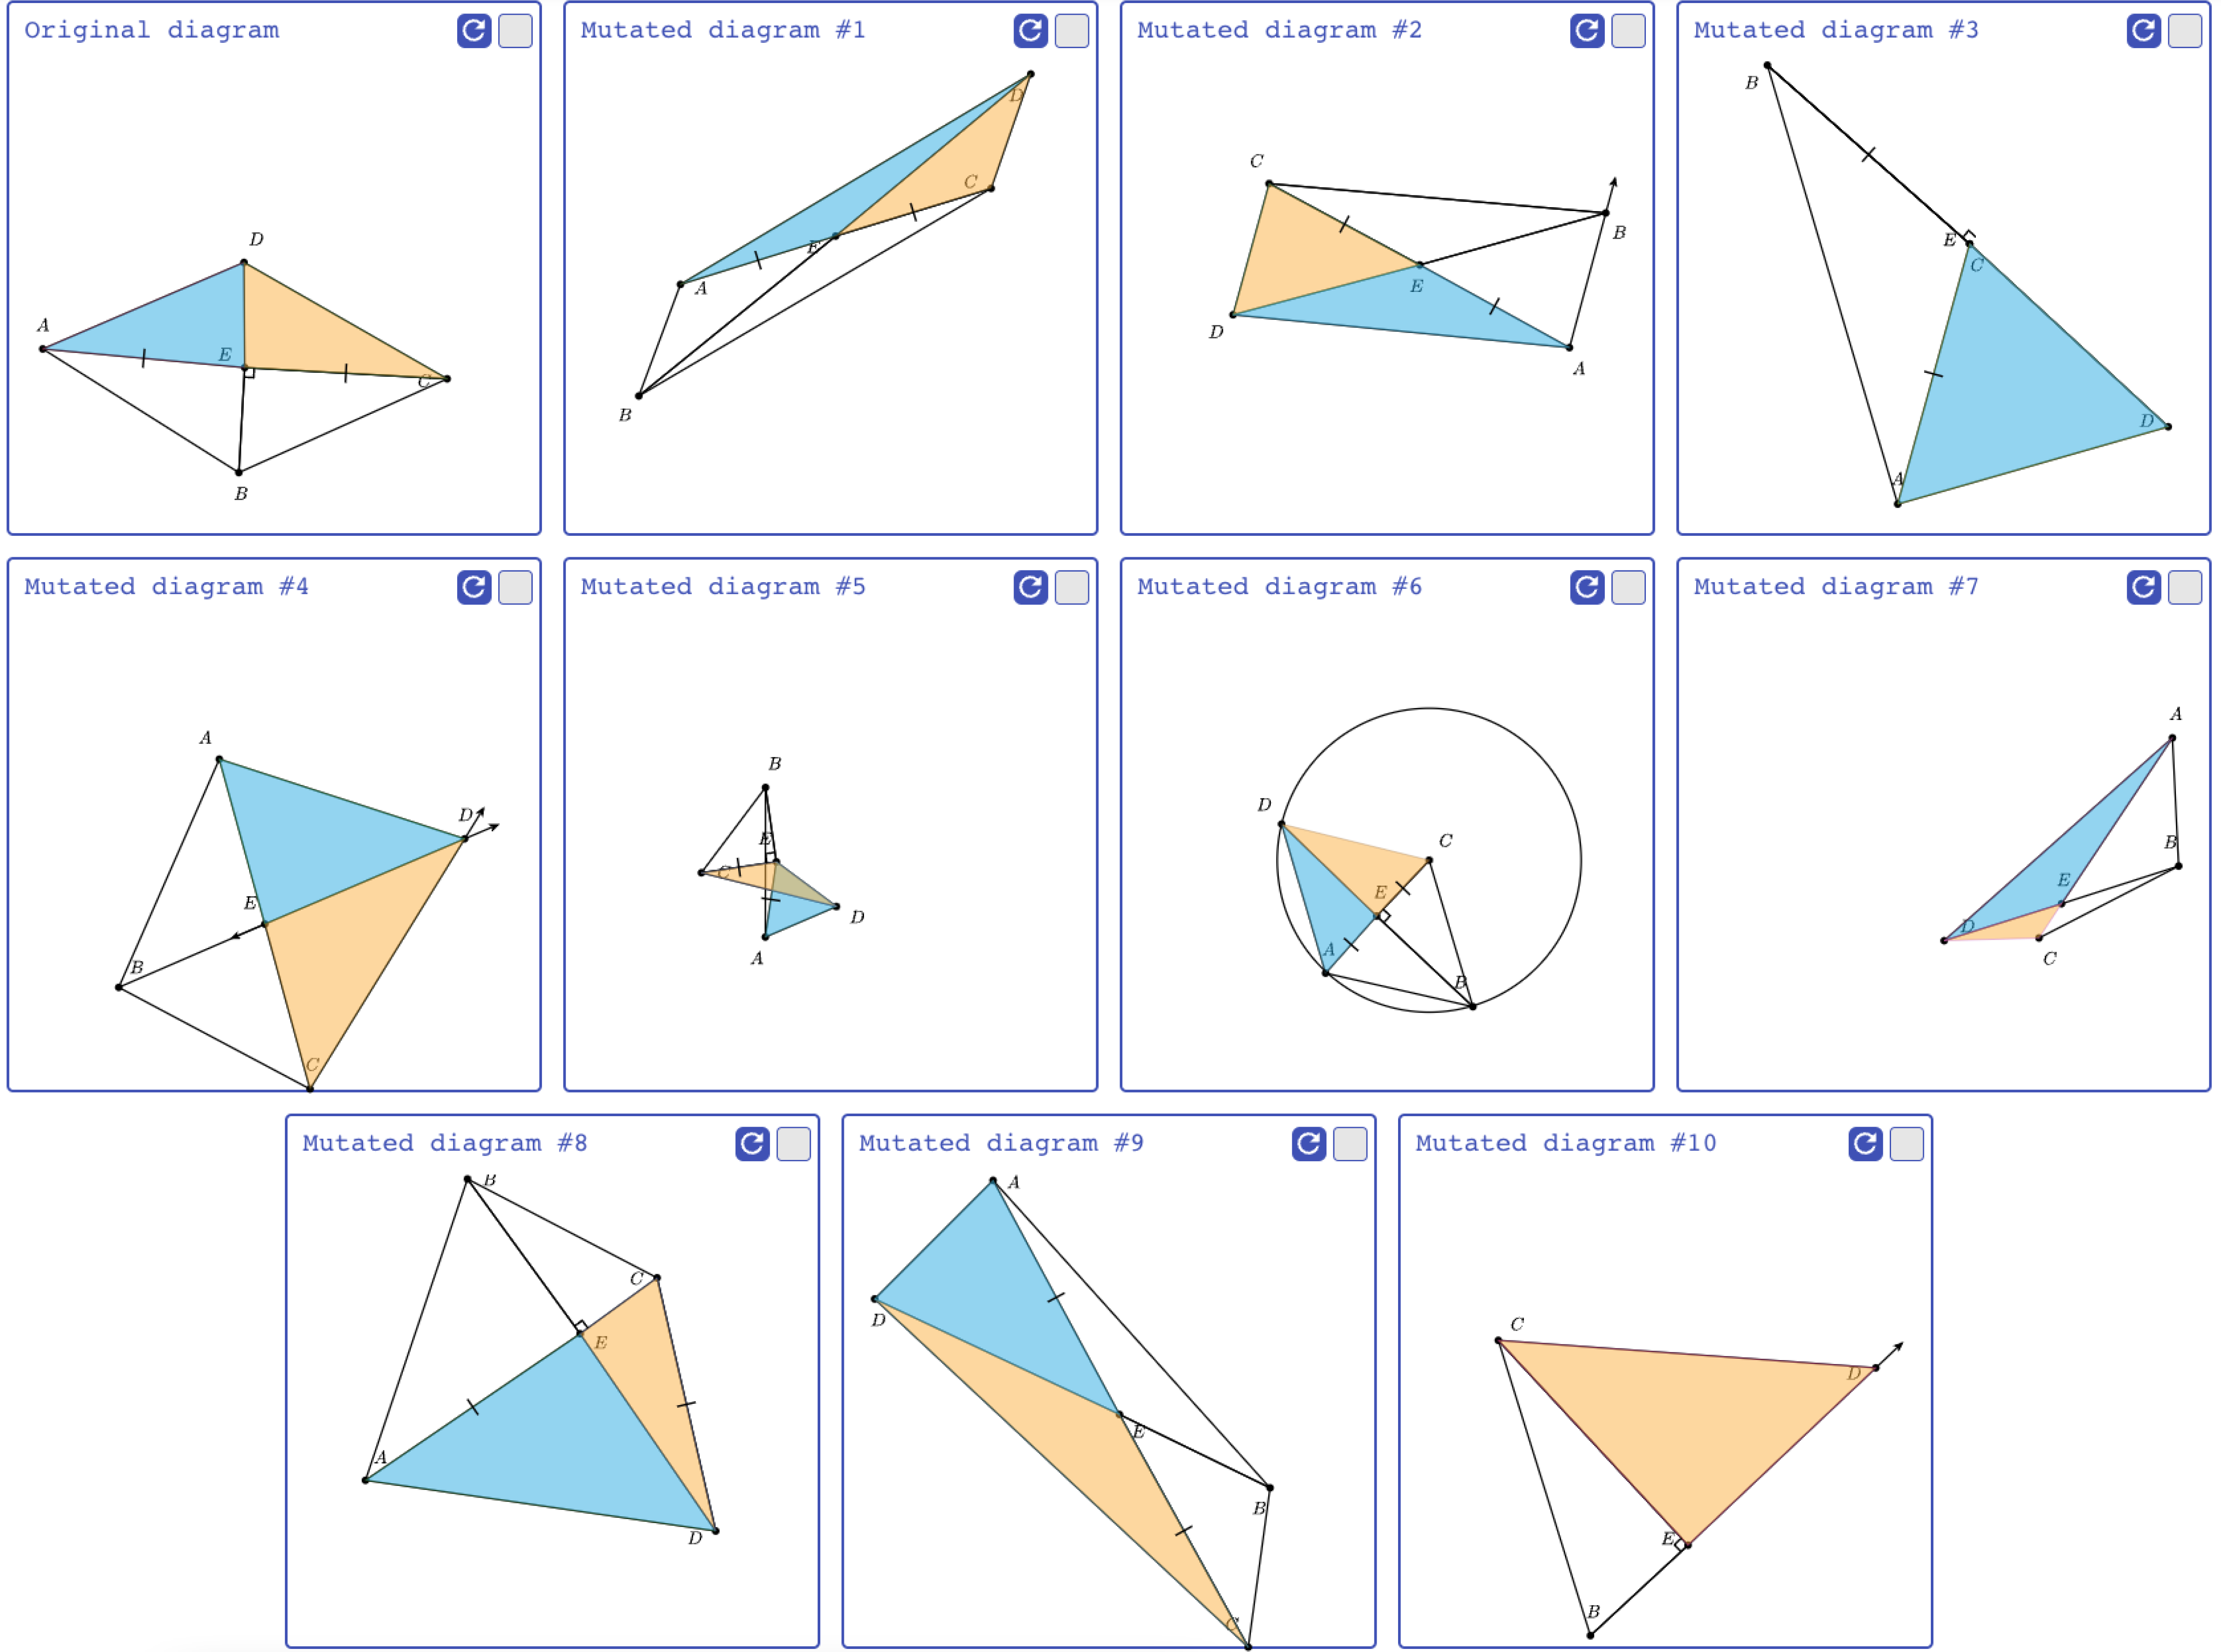
\includegraphics[width=\linewidth]{assets/edgeworth/geometry-grid.png}
    \caption{\textmd{The first ten diagram variations generated by \Edgeworth for the problem shown in \cref{fig:edgeworth-problems} (left).}}
    % \Description{This figure shows a grid of ten diagrams generated by Edgeworth given the example scenario in Figure 3 and 5. Some of the diagrams show congruent triangles DEA and DEC, while others show incongruent triangles.}
    \label{fig:geometry-grid}
\end{figure}

% \begin{figure}[h]
%     \centering
%     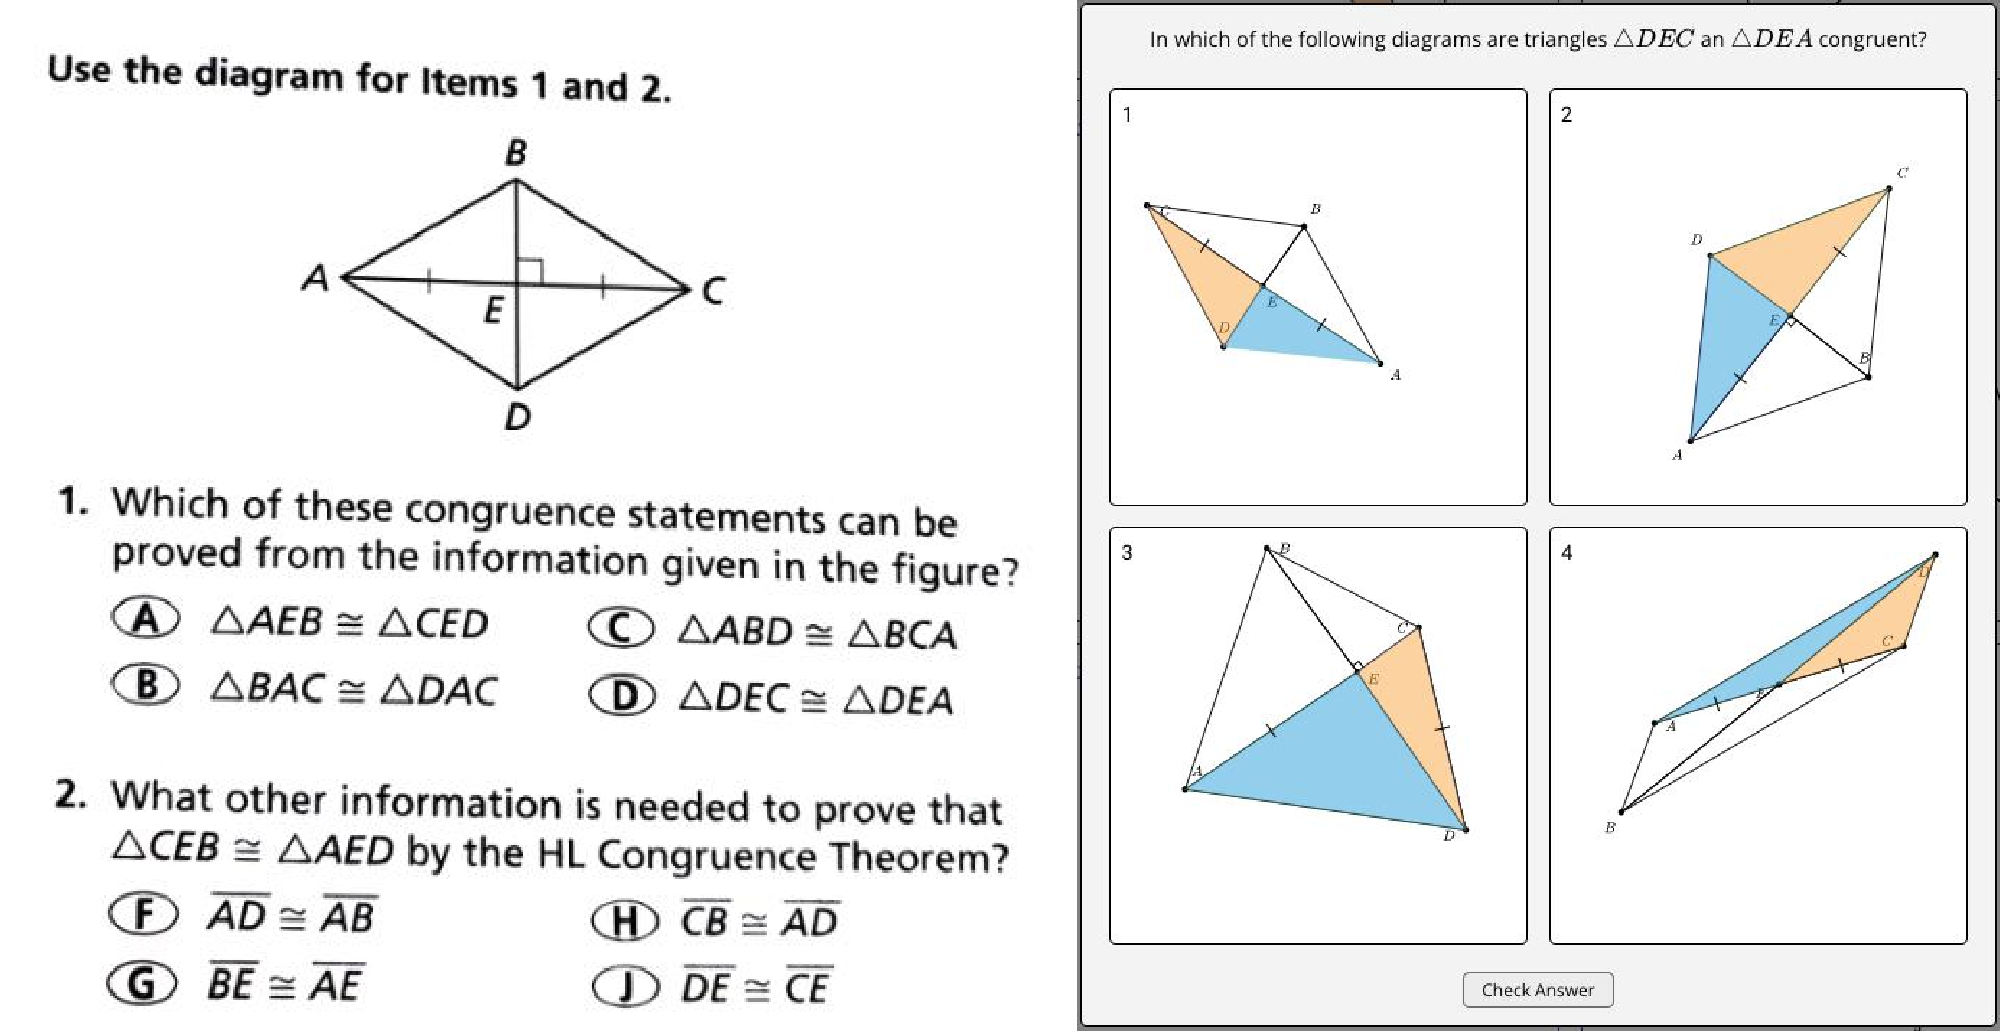
\includegraphics[width=\linewidth]{assets/geometry-problem.png}
%     \caption{An example problem in Holt \textit{Geometry}~\cite{burger2007holt} about triangle congruence (left) replicated in \Edgeworth (right). Colored shadings are added for clarity.}
%     \label{fig:geometry-problem}
% \end{figure}
We sample 17 Euclidean geometry problems from Holt \textit{Geometry} \cite{burger2007holt}, a high school geometry textbook. \cref{fig:edgeworth-problems} (left) shows an example problem. The textbook uses a consistent visual style of predominantly black line segments and dots with text labels. Most diagrammatic problems are presented as one diagram followed by one or more multiple-choice problems. We've recast the problems as diagrammatic translation problems.

For this domain, we build on the existing geometry stylesheet from \Penrose \cite[Section~5.3]{penrose} for diagram layout. In this domain, \Edgeworth weights deletions 20\% and edits 80\%. There are many different types of entities in geometry, so additions tend to introduce elements to the diagram that obviously do not pertain to the question prompt. Thus in this domain, the \Edgeworth mutator applies no additions. The reason we weight edits higher than deletions is that many of our geometry problems ask about specific named points, and deletions can make the diagram invalid by removing points that are mentioned in the prompt.

% \begin{wrapfigure}{r}{0.5\textwidth}
% \begin{figure}
%     \begin{center}
%         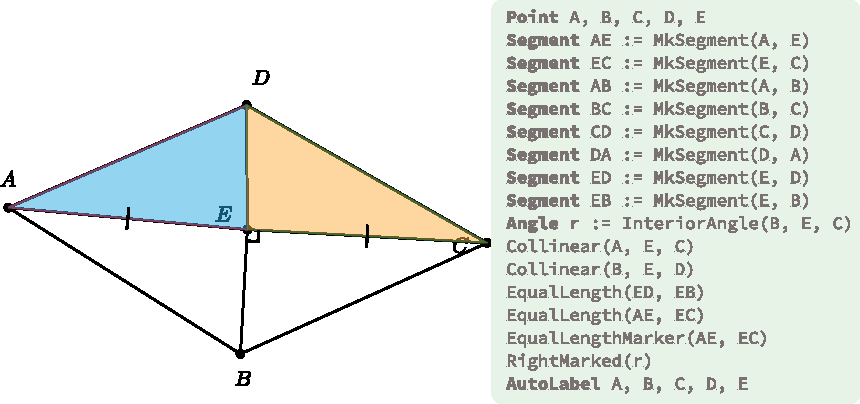
\includegraphics[width=\linewidth]{assets/congruence-example.pdf}
%     \end{center}
%     \caption{The example scenario of an Euclidean geometry problem.}
%     % \Description{This figure shows the diagram and Substance description of the example scenario in Figure 3. The diagram and Substance are identical to Figure 3.}
%     \label{fig:congruence-example}
% \end{figure}

% two-col
% \begin{figure}
%     \centering
%     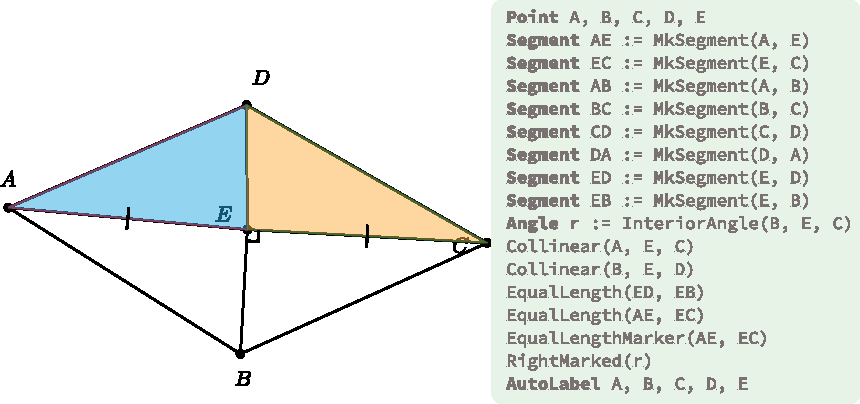
\includegraphics[width=\linewidth]{assets/congruence-example.pdf}
%     \caption{The example scenario of a Euclidean geometry problem.}
%     \Description{This figure shows the diagram and Substance description of the example scenario in Figure 3. The diagram and Substance are identical to Figure 3.}
%     \label{fig:congruence-example}
% \end{figure}

We use the problem in \cref{fig:edgeworth-problems} (left) to demonstrate how \Edgeworth generates variations that are meaningful as problem options. In the diagram shown, $\triangle DEC$ and $\triangle DEA$ are congruent by the Side-Angle-Side rule. In particular, they share a side ($DE$), the sides $AE$ and $EC$ appear to have equal length and are marked as such with a tick, and $\angle DEA$ and $\angle DEC$ are both right angles and therefore equal. 
% The diagram in \cref{fig:congruence-example} is replicated as Option 2 in \cref{fig:edgeworth-problems}. 
Option 4 in \cref{fig:edgeworth-problems} involves mutating the scenario by removing the right angle marker which makes it impossible to prove that $\angle DEA$ and $\angle DEC$ are equal. This is an example of the \textbf{Delete} mutation described in Section \ref{sec:edgeworth-mutation}. The angle appears to be a right angle in Option 3, so this option might serve as a good distractor for students still learning the distinction between the appearance of angles and their markings.

Option 3 involves mutating Option 2 by editing which sides have equal length. In Option 3, sides $CD$ and $AE$ are equal instead of $AE$ and $CE$. This is an example of the \textbf{Replace Arguments} mutation described in \cref{sec:edgeworth-mutation}. A student might incorrectly select Option 3 if they believed in a Side-Angle congruence rule, where a single angle and single side being equal could prove congruence. Finally, in Option 1 $\angle CEB$ neither is marked as a right angle nor appears as a right angle. A student might incorrectly select Option 1 if they believed in a Side-Side congruence rule, where two sides being equal could prove congruence.

\cref{fig:geometry-grid} shows the first 10 variations \Edgeworth generated from the example diagram. To create our problem, shown in \cref{fig:edgeworth-problems} (left), we selected the original diagram and two incorrect variations (numbers 1 and 8), plus another variation in an extended pool (number 16). As shown in \cref{fig:geometry-grid}, there are many other viable answer choices in the first 10 variations. Many of the diagrams involve extra details that are irrelevant to the problem, like the circle in number 6 or the vector above point B in number 2. These extra details can be pedagogically useful for teaching students to filter irrelevant information in the domain. Some of the other diagrams are very obviously incorrect, like number 10 which doesn't show a blue triangle, or number 7 where the blue triangle is much larger than the orange triangle; these can be useful for building confidence when students are first learning. 

% We assembled these problems from the diagrams alone. We did not look at the changes made to the textual scenario, and we do not expect our users to look at those textual changes. 

% \begin{figure}
%     \centering
%     \includegraphics[width=\linewidth]{assets/incorrect-mutants.pdf}
%     \caption{Three incorrect mutants (number 1, 8, and 16) selected for an Euclidean geometry problem (c04p01).}
%     \label{fig:incorrect-mutants}
% \end{figure}

% \cref{fig:incorrect-mutants} shows how \Edgeworth mutates the example scenario. For mutant 1, \Edgeworth changed \sub{RightMarked(r)} to make $\angle BEC$ an obtuse angle, thereby violating the SAS rule. The resulting diagram is visually obvious because the colored triangles clearly have different shapes. Mutant 8 violates another predicate \sub{EqualLength(AE, EC)} indirectly by changing the definition of $\overline{EC}$ to mean $\overline{CD}$. This is done by a combination of \textbf{Swap} and \textbf{Swap-In} mutations. The result is also a visually obvious incorrect diagram. Finally, mutant 18 changes \sub{RightMarked(r)} to \sub{RightUnmarked(r)} and also includes an irrelevant mutation that deletes $\overline{AD}$. Since the triangles are shaded, this extra mutation doesn't impact the readability of the resulting diagram. In fact, because $\angle BEC$ is still a right angle but not visually marked, it is a good distractor option for the problem. 




\subsection{General Chemistry: Lewis Structures}
\label{sec:chemistry}

% \begin{figure}[h]
%     \centering
%     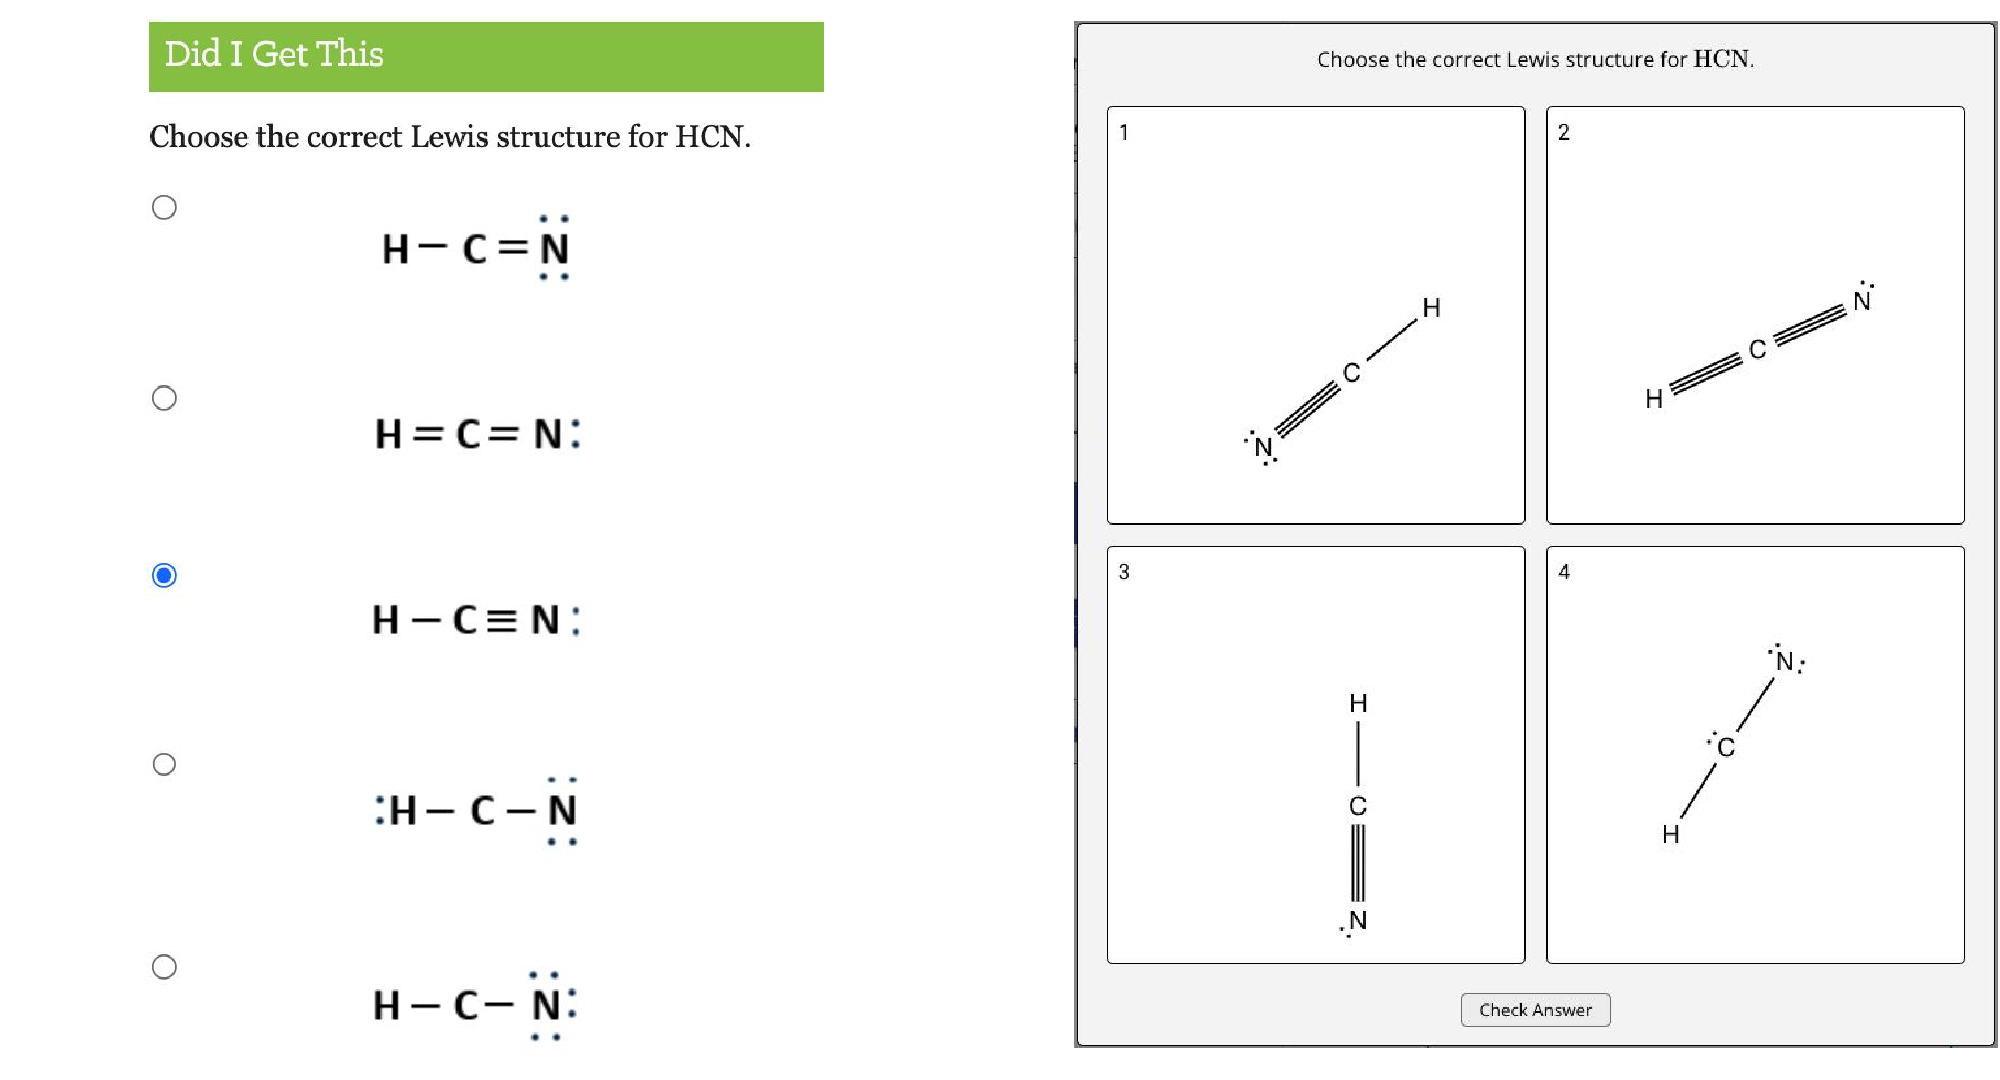
\includegraphics[width=\linewidth]{assets/chemistry-problem.png}
%     \caption{An example problem in general chemistry that asks the student to identify the correct Lewis structure for HCN.}
%     \label{fig:chem-problem}
% \end{figure}

We chose 7 chemistry problems on Lewis structure from an online General Chemistry 1 course \cite{oli}. These problems test students' understanding of how atoms bond together based on formal charges. The module introduces students to the \textit{octet rule}: the tendency of main group atoms to form enough bonds to obtain eight valence electrons. Lewis structure diagrams show bonds among atoms and valence electrons on atoms typically following the octet rule. 

% To accurately assess student understanding and give them appropriate varied practice, it is important that problems (and solution options) in this module differentiate student understanding of these more particular principles:

% \begin{itemize}
%     \item The number of valence electrons in the outer shell is determined by the atomic number.
%     \item The most common molecular configuration minimizes free electrons. 
% \end{itemize}

We extend the existing \Penrose chemistry stylesheet to include notation and layout rules for Lewis structures. To permit incorrect diagrams, the chemistry stylesheet must not enforce the octet rule. It does specify that an atom can have any number of bonds and that it can have 0, 2, 4, or 6 valence electrons. These specifications cover all problem scenarios in this Lewis structure module.\footnote{``Odd electron molecules are very rare and cannot achieve full octets of electrons around atoms because of the odd number of electrons.'' \cite{oli}} In accordance with stylistic conventions in the field, \Edgeworth automatically lays out atoms, bonds, and electrons to maximize bond angles and repel electrons from bonds 
% (\eg \cref{fig:cocl2-example} and \cref{fig:edgeworth-problems} bottom-middle)
. For molecules involved in all 7 problems, the layout algorithm produces high-quality diagrams without any manual manipulation needed from the author. 

To configure \Edgeworth for this domain, we weight edits 100\%. We exclusively weight on edits because we observed that variations of molecules never add or delete atoms and bonds. Although valence electrons may be added or deleted, they are modeled as predicates that can be edited to change the number of electrons for an atom (\eg \sub{ZeroDots(H)} $\rightarrow$ \sub{TwoDots(H)}) via a \textbf{Replace Function} mutation operation. 

Figure~\ref{fig:edgeworth-problems} (middle) shows an \Edgeworth Lewis structure problem for hydrogen cyanide, with the correct diagram in the top-left. Incorrect choices for this problem can be generated via mutation. For instance, if a student forgets that nitrogen must have eight surrounding electrons, they might choose the bottom-left option, which was generated by removing the valence electrons around nitrogen. Or, if a student does not know that hydrogen should only have two electrons instead of eight, they might select the top-right choice, which was generated by mutating the number of electrons around hydrogen from zero to six. Finally, if a student does not know that free electrons should be minimized, they might pick the bottom-right diagram, which was generated by mutating up the number of electrons around carbon and nitrogen and changing the triple bond to a double bond.

\subsection{Discrete Math: Graphs}
\label{sec:graphs}

% \begin{figure}[h]
%     \centering
%     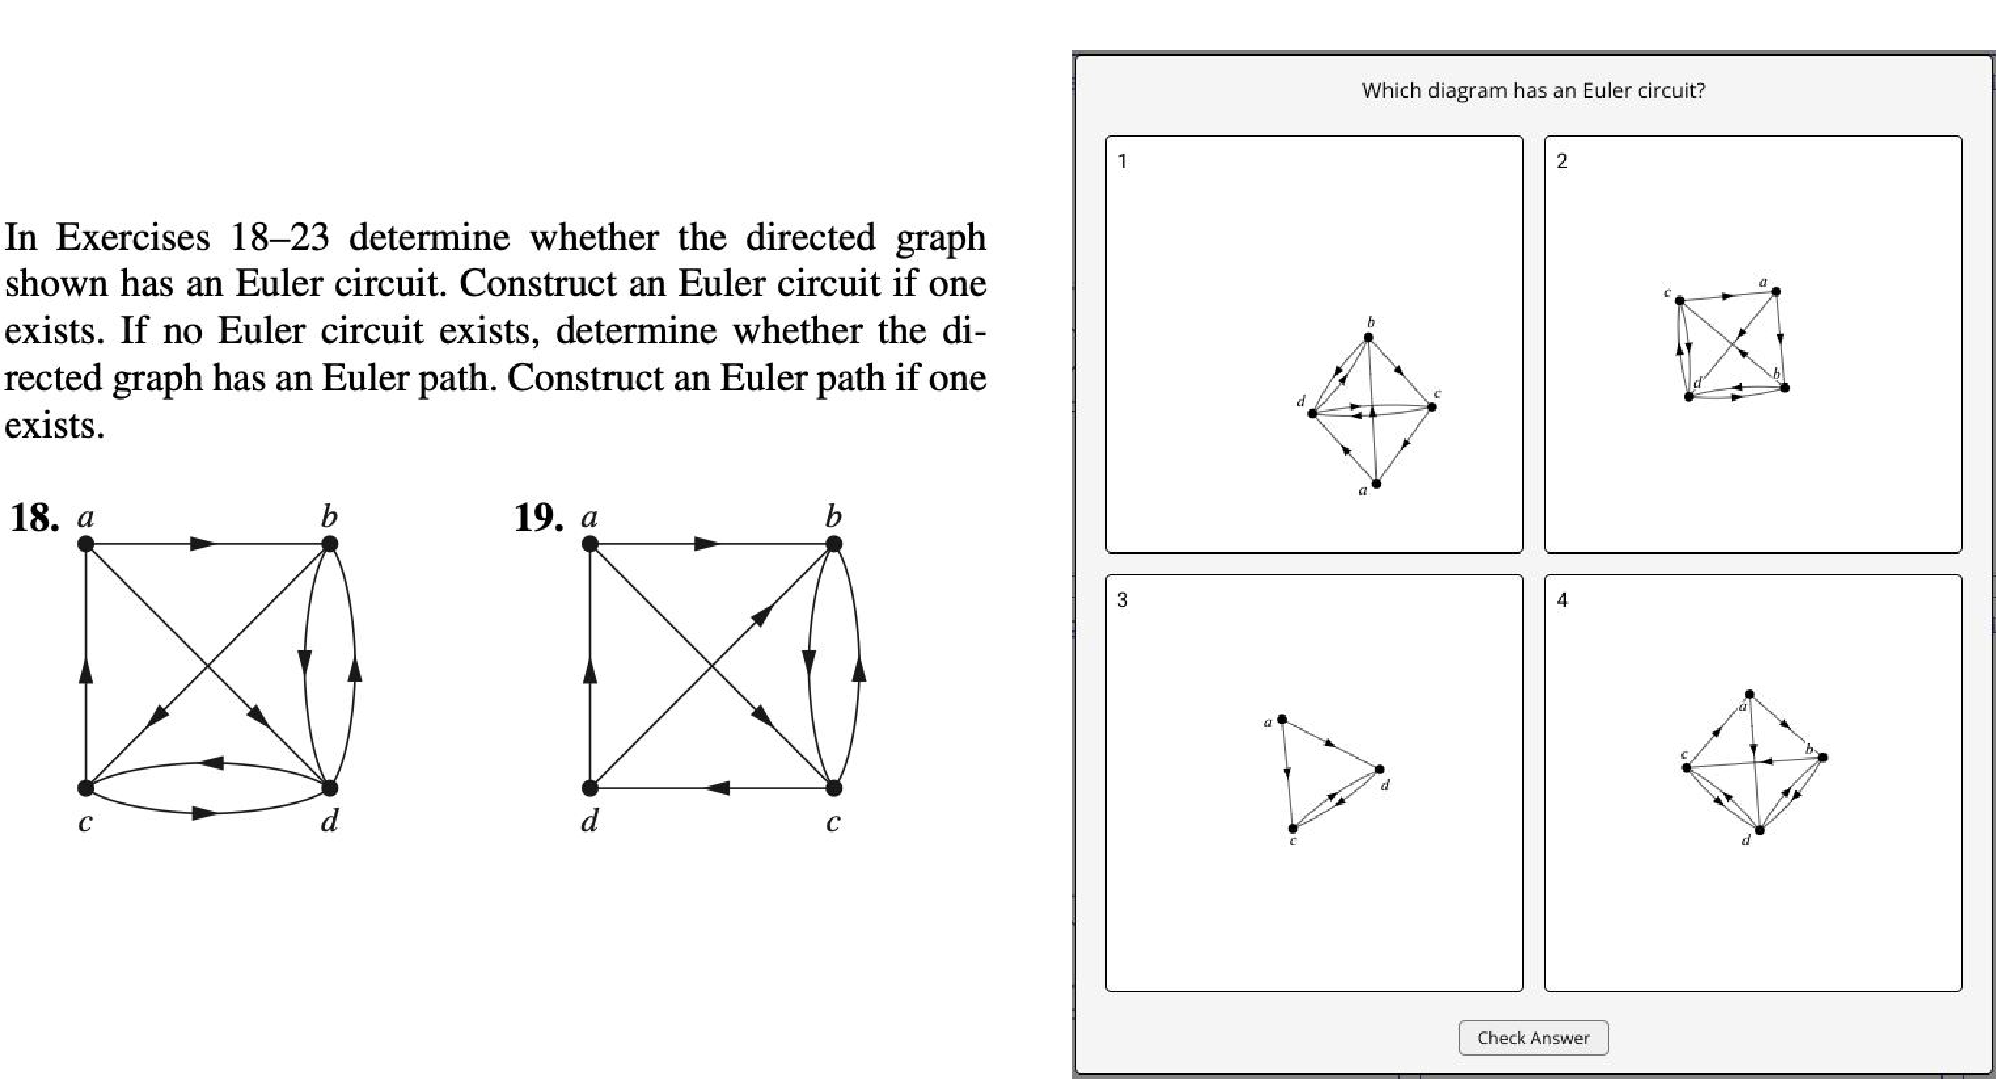
\includegraphics[width=\linewidth]{assets/graph-problem.png}
%     \caption{An example problem that asks the student to identify graphs with Euler circuits.}
%     \label{fig:chem-problem}
% \end{figure}

We draw 7 graph theory problems from the ``Graphs'' chapter of \textit{Discrete Mathematics and Its Applications} \cite[Chapter~10]{rosen1999discrete}.  We model our visual representation after the style used in the textbook, allowing students to recognize \Edgeworth-generated diagrams as they are already accustomed to recognizing graph diagrams. We created a new \Penrose stylesheet for four subdomains of graphs (directed vs not, and multigraph vs not). For each of these subdomains, \Edgeworth automatically lays out graph nodes, edges, loops, arrows, and labels in configurations that minimize confusing overlap of diagram elements. As with the other domains, no manual tweaking is necessary to obtain high-quality diagrams for problem variations. 
% The book defines six subdomains in Section 10.1, of which we use four:
% \begin{itemize}
%     \item \textit{Simple graph}---single undirected edges, no loops
%     \item \textit{Pseudograph}---multiple undirected edges, loops allowed
%     \item \textit{Simple directed graph}---single directed edges, no loops
%     \item \textit{Directed multigraph}---multiple directed edges, loops allowed
% \end{itemize}


To configure \Edgeworth for the graph domain, we weight additions 50\%, deletions 40\%, and edits 10\%. We disfavor edits in this domain because most of them are not useful: \textbf{Replace Function} is inapplicable for any of our graph subdomains, and \textbf{Swap Arguments} only applies to directed graphs. \textbf{Replace Arguments} is meaningful, but most desirable mutations for graphs are better represented by the addition or deletion of edges, or sometimes nodes. For instance, a bipartite graph can become not-so by adding edges, or a strongly-connected graph can become not-so by deleting edges. 

Figure~\ref{fig:edgeworth-problems} (right) shows an \Edgeworth problem asking which of four directed graphs have an Euler circuit. The bottom-right diagram does not have an Euler circuit, as can be seen by observing that the sum of $a$'s in-degree and out-degree is odd. In contrast, for the diagram in the bottom-left generated by deleting edge $(a, d)$, every node has an even sum of in-degree and out-degree, and indeed there does exist an Euler circuit. This condition on degree is only sufficient for undirected graphs, though; the diagram in the top-right is generated by flipping edge $(b, c)$ from the bottom-left diagram, but does not have an Euler circuit, thwarting the simple degree counting heuristic. Finally, the simple diagram in the top-left is generated by deleting $d$ and trivially has an Euler circuit. 

% \section{Summary}

% TODO



\chapter[Evaluating \Edgeworth{}]{Evaluating \Edgeworth{}\footnote{This chapter is partly adapted from Sections~6 to 7 of ``\citefield{ni_edgeworth_2024}{title}''~\cite{ni_edgeworth_2024}.}}
\label{chp:edgeworth-eval}
In this chapter, we discuss three studies to evaluate various aspects of \Edgeworth (\cref{chp:edgeworth}). To effectively scale up visual practice authoring, \Edgeworth must support a diverse set of instructional domains, generate high-quality diagrams consistently, and allow educators to author real-world problems. In \cref{sec:edgeworth-user-study,sec:reliability-eval,sec:expert-feedback}, we evaluate \Edgeworth by answering the following research questions on these qualities:

% self-contained RQs
% \refstepcounter{rqsupcounter}\label{rq:mut}
% \refstepcounter{rqsupcounter}\label{rq:eff}
% \refstepcounter{rqsupcounter}\label{rq:eco}


\begin{itemize}
    \item\textbf{Reliability} (\ref{rq:mut}): Can \Edgeworth reliably generate translation problems within relatively few diagram variations?
    \item\textbf{Efficiency} (\ref{rq:eff}): comparing with a conventional drawing tool, are authors more efficient at making translation problems using \Edgeworth? 
    \item\textbf{Ecological validity} (\ref{rq:eco}): Do real-world instructors consider \Edgeworth-generated translation problems to be useful? 
\end{itemize}

First, we evaluated the reliability of \Edgeworth by labeling 310 diagram variations from translation problem dataset (\cref{sec:edgeworth-case-studies}) by hand. With high inter-rater reliability ($\kappa=1$), the result shows that \Edgeworth can reliably generate diagrams that constitute valid four-choice translation problems, when constrained to 10 variations per problem.

Second, we performed a user study to measure authors' efficiency at creating translation problems using \Edgeworth, compared with a conventional drawing tool. The results show that once authors make a correct diagram, they are about 3 times faster at making diagrammatic options for translation problems using \Edgeworth compared to Google Drawings. 

Finally, we conducted walkthrough demonstrations with 9 educators that have experience creating problems. The goal of the demonstrations was to obtain feedback on the ecological validity of \Edgeworth-generated problems and the usefulness of \Edgeworth in general. Overall, these experts found \Edgeworth-generated problems to contain pedagogically useful variations and high visual quality. They provided detailed feedback on individual diagram variations and suggested how \Edgeworth might fit into their instructional contexts. 

\section{Reliability Evaluation (\ref{rq:mut})}
\label{sec:reliability-eval}

\Edgeworth's approach involves random mutations. The mutation operations are type-safe, but type-safety does not prevent degenerate diagram layouts. For instance, \sub{Point A, B} followed by \sub{Triangle t := MkTriangle(A, A, B)} will typecheck. However, since the triangle described in this scenario involves the \sub{Point A} twice, \Edgeworth will produce a line segment, not a triangle from this scenario. Are \Edgeworth suggestions dominated by these nonsensical scenarios? In this section, we evaluate whether \Edgeworth can reliably suggest diagrams that are valid answer options to multiple-choice translation problems (\ref{rq:mut}). 

\subsection{Methods}
\label{sec:reliability-method}

The goal of \Edgeworth is to generate enough diagram variations to assemble a four-choice multiple-choice problem for a given prompt. To this end, we use the following classification scheme for diagram variations: a variation can be a \textbf{Correct} or \textbf{Incorrect} answer to the prompt, or \textbf{Discard}ed because the diagram is invalid for missing key components or lacking readability.

For \ref{rq:mut}, we define ``relatively few variations'' to be 10 diagrams, and consider \Edgeworth to have generated a translation problem in $n$ variations if at that point we have (possibly including the original diagram) at least one \textbf{Correct} diagram, at least one \textbf{Incorrect} diagram, and in total at least four diagrams that are either \textbf{Correct} or \textbf{Incorrect}.

We used \Edgeworth to generate 10 diagrams per problem for all 31 problems in the translation problem dataset (\cref{sec:edgeworth-case-studies}), which yielded 310 diagrams in total. To evaluate this coding scheme, we randomly sampled 2 problems from each of our 3 domains, for 60 generated diagrams total. The first two authors each coded all 60 of those sample diagrams, after which we calculated the Cohen's $\kappa$ \cite{cohen1960coefficient} statistic. Then with the assumption that our coding scheme has reasonable inter-rater reliability, at least one author\footnote{The study is conducted jointly with authors of~\citet{ni_edgeworth_2024}.} coded all remaining diagrams, allowing us to determine the number of our prompts for which \Edgeworth was able to successfully generate a multiple-choice problem. The coding results are included in \cref{app:reliability}.

\subsection{Results}

\subsubsection{Reliability of Problem Generation}

For \ref{rq:mut}, we found that \Edgeworth generated valid multiple-choice problems for 27/31 prompts within 10 variations, and for 30/31 problems within 20 variations. For each of these four failures with 10 variations, \Edgeworth did generate at least four \textbf{Correct} examples, but we had to \textbf{Discard} all the other diagrams, leaving no \textbf{Incorrect} examples. For the one remaining failure with 20 variations, \Edgeworth never succeeded even after we increased the number of variations to 50.


\subsubsection{Distribution}

\begin{table}
    \centering
    \begin{tabular}{r|rrr|r}
        & \textbf{Correct} & \textbf{Incorrect} & \textbf{Discard} & \textit{total} \\
        \hline
        geometry & 52 & 54 & 64 & 170 \\
        chemistry & 3 & 54 & 13 & 70 \\
        discrete & 28 & 25 & 17 & 70 \\
        \hline
        \textit{total} & 85 & 133 & 94 & 310
    \end{tabular}
    \caption{Distribution of diagram variation classes.}
    % \Description{This table describes the coding results from the reliability evaluation. There are four rows (blank, geometry, chemistry, discrete, and total) and five columns (blank, correct, incorrect, discard, and total). The first row and first column contain the headers. The numbers starting from row 2, column 2, in row order are: Row 2: 52, 54, 64, 170; Row 3: 3, 54, 13, 70; Row 4: 28, 25, 17, 70; Row 5: 85, 133, 94, 310}
    \label{tab:distribution}
\end{table}

The original diagram is a \textbf{Correct} answer for every prompt, except for the two Euler circuit prompts, in which the original diagram is \textbf{Incorrect}. For \Edgeworth-generated variations, the full distribution of classes is shown in Table~\ref{tab:distribution}.

The chemistry domain had a far smaller proportion of \textbf{Correct} variations than the other two domains because the only way for a variation to be \textbf{Correct} is for it to coincidentally be identical to the original diagram. Interestingly, in the other two domains, there were about the same number of \textbf{Correct} and \textbf{Incorrect} variations.

In the geometry domain, \textbf{Discard}ed diagrams were primarily either diagrams missing elements referred to in the question prompt, or diagrams that were visually degenerate (\eg everything compressed into a single line). In chemistry, we \textbf{Discard}ed diagrams where the molecule was disconnected. Finally, in the graph domain, we \textbf{Discard}ed diagrams in which some nodes were labeled and others were unlabeled (\ie \Edgeworth had inserted new unlabeled nodes when all nodes in the original diagram were labeled).

\subsubsection{Inter-rater Agreement}

We sampled two problems per domain from the problems collected in ~\cref{sec:edgeworth-case-studies} to evaluate inter-rater agreement (six problems or sixty diagrams in total, 19\% of the dataset). We found perfect agreement on that sample, so $\kappa = 1$.

\section{Experimental Evaluation of Authoring Efficiency (\ref{rq:eff})}
\label{sec:edgeworth-user-study}

To answer \ref{rq:eff}, we conduct an experiment that compares \Edgeworth against a conventional drawing tool in translation problem authoring tasks. In this section, we describe the experimental setup and findings.

\subsection{Study Design}


\subsubsection{Participants}

We recruited 16 participants through advertisement in the university community (e.g. emails and Slack channels). Participants were screened to have some past experience using digital drawing tools. All participants reported that they have used Google Drawings and/or equivalent tools to make diagrams in the past.

\subsubsection{Tasks}
\label{sec:edgeworth-user-tasks}

\begin{figure}
    \centering
    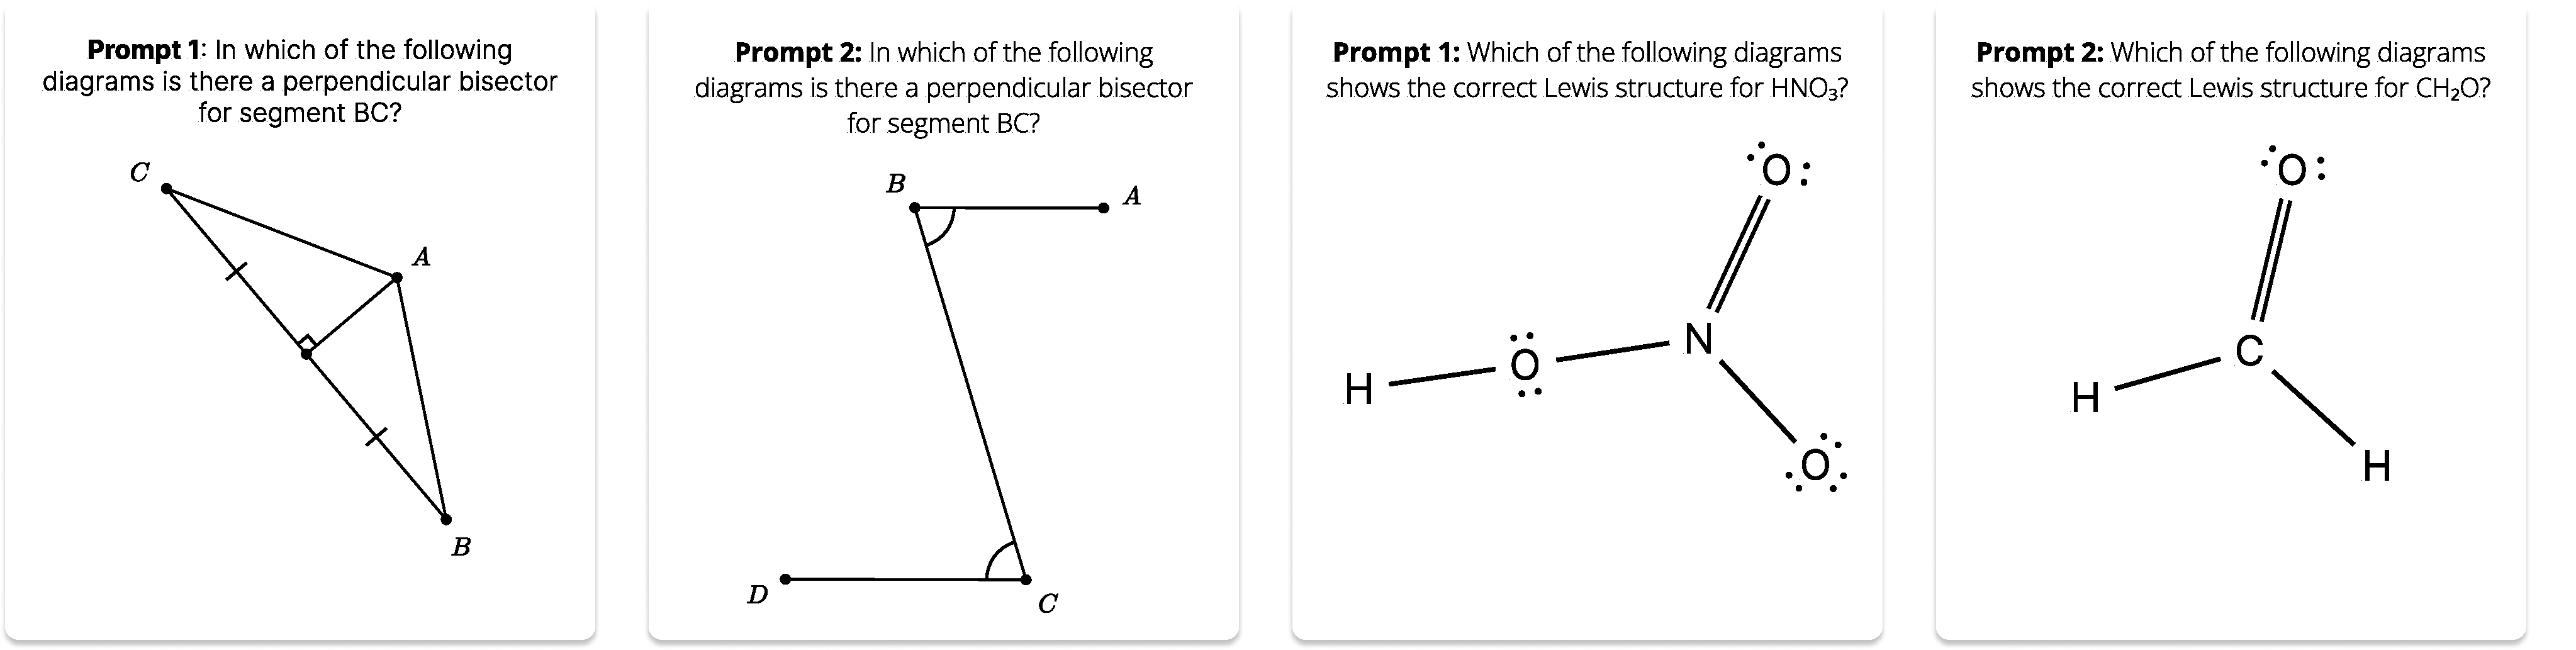
\includegraphics[width=\linewidth]{assets/edgeworth-eval/user-study-tasks.pdf}
    \caption{Tasks used in the \Edgeworth experimental evaluation. Each participant is given a textual prompt and a correct diagram to this prompt at the beginning of each task. They are asked to first re-produce the correct diagram using the designated tool in the correct segment, and then edit this diagram to produce up to 10 incorrect diagrams to the prompt in the incorrect segment.}
    \label{fig:edgeworth-user-study-tasks}
\end{figure}

We selected four problem prompts from the translation problem dataset (\cref{sec:edgeworth-case-studies}), two from the chemistry domain and two from geometry, shown in \cref{fig:edgeworth-user-study-tasks}.

We segmented the authoring of the first correct diagram and subsequent incorrect diagrams in the tasks. This segmentation allows us to separately measure the authoring efficiency of creating the example scenario (\cref{sec:create-scenario}) and creating counterexamples (\cref{sec:select-diagrams}). For participants who used \Edgeworth, we were particularly interested in the upfront cost of making the first \Substance diagram in the \Penrose editor. 

For each task, the participant were given (1) a textual problem prompt and (2) an example diagram (\ie a correct response to the prompt). Participants were then given up to 20 minutes to complete each task, which involve two segments: (a) \textbf{correct segment}: participants first re-created one example visually similar to the given diagram and then (b) \textbf{incorrect segment}: made up to 10 incorrect diagrams by editing the diagram produced in sub-task (a). Each sub-task is time-bounded to 10 minutes. If the participant failed to produce 1 correct diagram in the first segment, they were provided with one so they could continue to the next segment. Each participant completed two problem prompts in chemistry or geometry. 

\subsubsection{Experimental Design}

\begin{table}[t]
\centering
\begin{tabular}{l|llllll}
Domain & Task 1 (Prompt 1) & Task 2 (Prompt 1) & Task 3 (Prompt 2) & Task 4 (Prompt 2)  \\ \hline
Chemistry &  Google Drawings & \Edgeworth & Google Drawings & \Edgeworth \\
Chemistry & \Edgeworth & Google Drawings & \Edgeworth & Google Drawings \\
Geometry &  Google Drawings & \Edgeworth & Google Drawings & \Edgeworth \\
Geometry & \Edgeworth & Google Drawings & \Edgeworth & Google Drawings \\
\end{tabular}
\caption{Participants were divided into 4 groups by the tools they used and diagramming domains of the tasks. Each row corresponds to the task sequence of one of the groups. Participants used both \Edgeworth and Google Drawings to author problems for two prompts in chemistry or geometry (\cref{fig:edgeworth-user-study-examples}).} \label{tab:edgeworth-experiment-groups}
\end{table}

% groups
The study was a within-subject design, where participants were divided into four groups by the ordering of tools they use and diagramming domains of their tasks. Participants used both \Edgeworth and Google Drawings to author diagrams in a random counterbalanced order. Participants were further randomly assigned into one of two subgroups: one subgroup made chemistry diagrams and the second subgroup made geometry diagrams. \cref{tab:edgeworth-experiment-groups} summarizes the four groups that resulted from the tool and domain assignments. Each group had four participants.

In the 90-minute study session, each participant was given two problem prompts in total, each repeated twice for \Edgeworth and Google Drawings, so four tasks in total. For instance, a participant in the chemistry-drawing group (the first row in \cref{tab:edgeworth-experiment-groups}) would spend up to 10 minutes making 1 correct diagram (correct segment) and then up to 10 minutes to make incorrect diagrams of \ensuremath{\mathrm{CH_2O}} using Google Drawings (incorrect segment) first, and then another 20 minutes on the same prompt using \Penrose for the correct segment and \Edgeworth for the incorrect segment. After that, this participant would repeat the same for  \ensuremath{\mathrm{HNO_3}}.



% authoring assistance

\begin{figure}
    \centering
    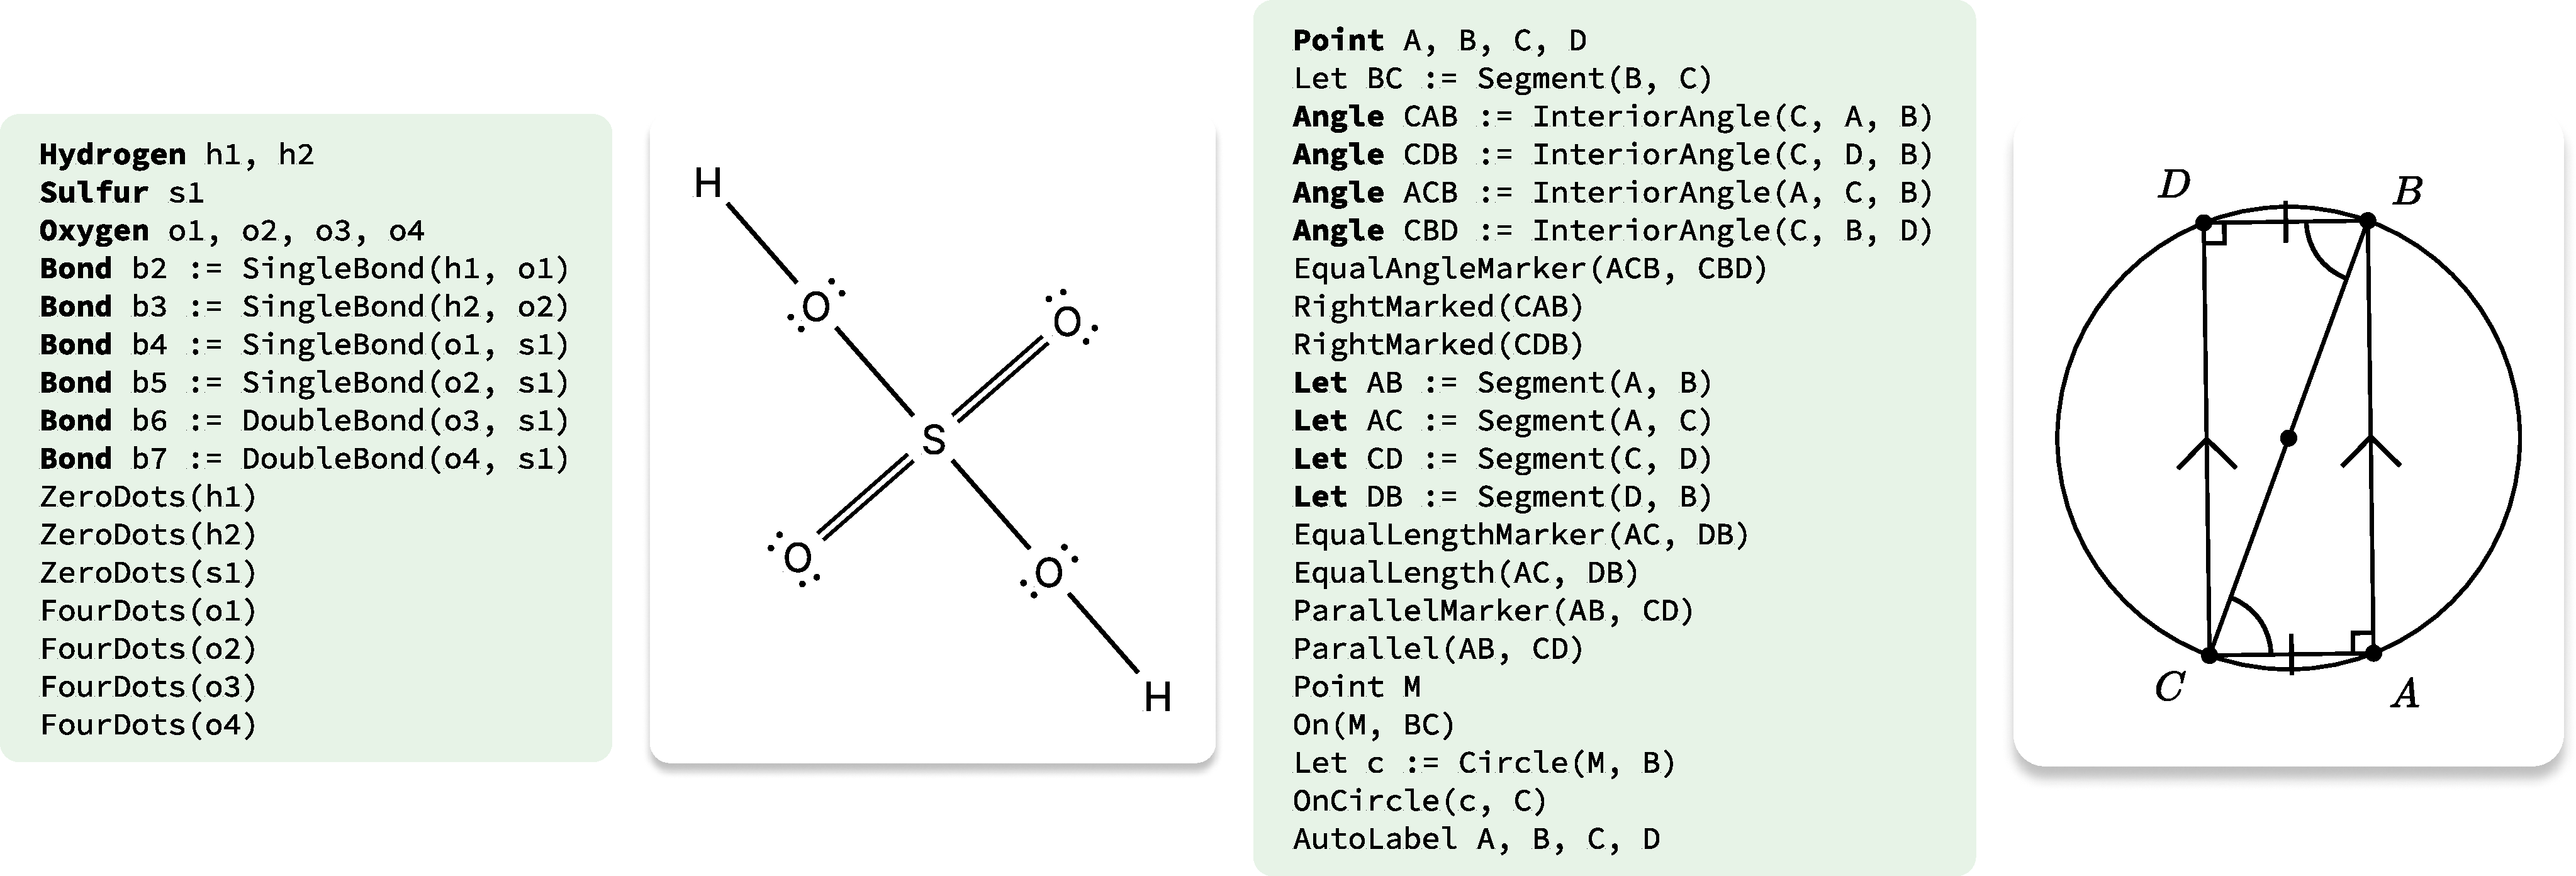
\includegraphics[width=\linewidth]{assets/edgeworth-eval/user-study-examples.pdf}
    \caption{Participants were provided both Google Drawings and \Substance examples throughout the study. The \SubstanceColored code (left) was given in the \Edgeworth tasks and a Google Drawings file that visually resembles the \Penrose output (right) was given for the Google Drawings tasks.}
    \label{fig:edgeworth-user-study-examples}
\end{figure}

At the start of each study session, participants were given 5-minute tutorials of \Edgeworth and Google Drawings, in which they were guided to draw either a right triangle or the Lewis structure of \ensuremath{\mathrm{O_2}}. The ordering of tutorials match the counterbalanced ordering of Google Drawings and \Edgeworth. Throughout the session, participants had access to one Google Drawings example and one \Substance example. \cref{fig:edgeworth-user-study-examples} shows the chemistry and geometry examples. The examples are samples from the translation problem dataset (\cref{sec:edgeworth-case-studies}) that are visually more complex than the actual study tasks. We provided them to the participants as an authoring aid so that they can copy elements from the examples to save time, analogous to the real-world experience of copying and pasting online examples reported in \cref{sec:edgeworth-formative}.

Participants received no more instructions during the tasks. The experimenter only observed the participant and used a stopwatch to measure the time on task. After completing each task, participants completed a survey that asked them if they agree with the following statements on a 5-point Likert scale:

\begin{itemize}
  \item I would use this problem for a class that I teach.
  \item The problem is pedagogically useful (\ie students will benefit from doing this problem).  
  \item The diagrams in the problem are of high visual quality.
\end{itemize}

The study took about 90 minutes per participant, using a provided MacBook Pro with the latest version of Chrome installed. The study sessions were audio-recorded and transcribed. All participants were compensated \$25 Amazon gift cards for their time.

\subsection{Results}

% completion
\cref{tab:edgeworth-user-study-timing} shows the average total time, diagrams produced, and time per diagram for all participants. The \textbf{Diagram Ct} column in \cref{tab:edgeworth-user-study-timing} shows how many diagrams participants produced in each segment of all tasks on average. Any number lower than 1 for correct segments and 10 for incorrect segments indicates that the corresponding participant did not complete the segment. 
All participants authored 10 incorrect diagrams within 10 minutes using \Edgeworth for both domains. In the geometry group, 6 out of 8 participants (11 out of 16 total segments) failed to do so using Google Drawings for at least one segment. In the chemistry group, 1 out of 8 participants failed for both incorrect segments. All participants were able to complete the correct diagram for both chemistry prompts using both tools. For the geometry tasks, all participants produced one correct diagram in the first segment using Google Drawings, but 3 failed using \Penrose. 

\begin{table}[h!]
\centering
\begin{tabular}{|l|l|l|r|r|r|}
\hline
\textbf{Domain} & \textbf{Segment} & \textbf{Tool} & \textbf{Total Time} & \textbf{Diagram Ct} & \textbf{Time/Diagram} \\ \hline
Chemistry & correct   & \Penrose        & 144.19s & 1.00  & 144.19s \\ \cline{3-6} 
          &           & Google Drawings & 231.81s & 1.00  & 231.81s \\ \cline{2-6}
          & incorrect & \Edgeworth      & 150.13s & 10.00 & 15.01s  \\ \cline{3-6} 
          &           & Google Drawings & 440.63s & 9.38  & 51.56s  \\ \hline
Geometry  & correct   & \Penrose        & 390.94s & 0.81  & 390.94s \\ \cline{3-6} 
          &           & Google Drawings & 228.50s & 1.00  & 228.50s \\ \cline{2-6}
          & incorrect & \Edgeworth      & 257.25s & 10.00 & 25.73s  \\ \cline{3-6} 
          &           & Google Drawings & 549.38s & 7.38  & 100.90s \\ \hline
\end{tabular}
\caption{Summary of Average Time, Diagram Count, and Time Per Diagram by Domain for both chemistry and geometry domains, and two segments of each task (\cref{sec:edgeworth-user-tasks}).}
\label{tab:edgeworth-user-study-timing}
\end{table}

% time
A two-way repeated measures ANOVA was conducted to examine the within-subject effects of tool (\Edgeworth vs. Google Drawings) and task (correct vs. incorrect) on various outcomes. The analysis included task completion time and other performance metrics across the domains of chemistry and geometry.

\begin{figure}[h]
    \centering
    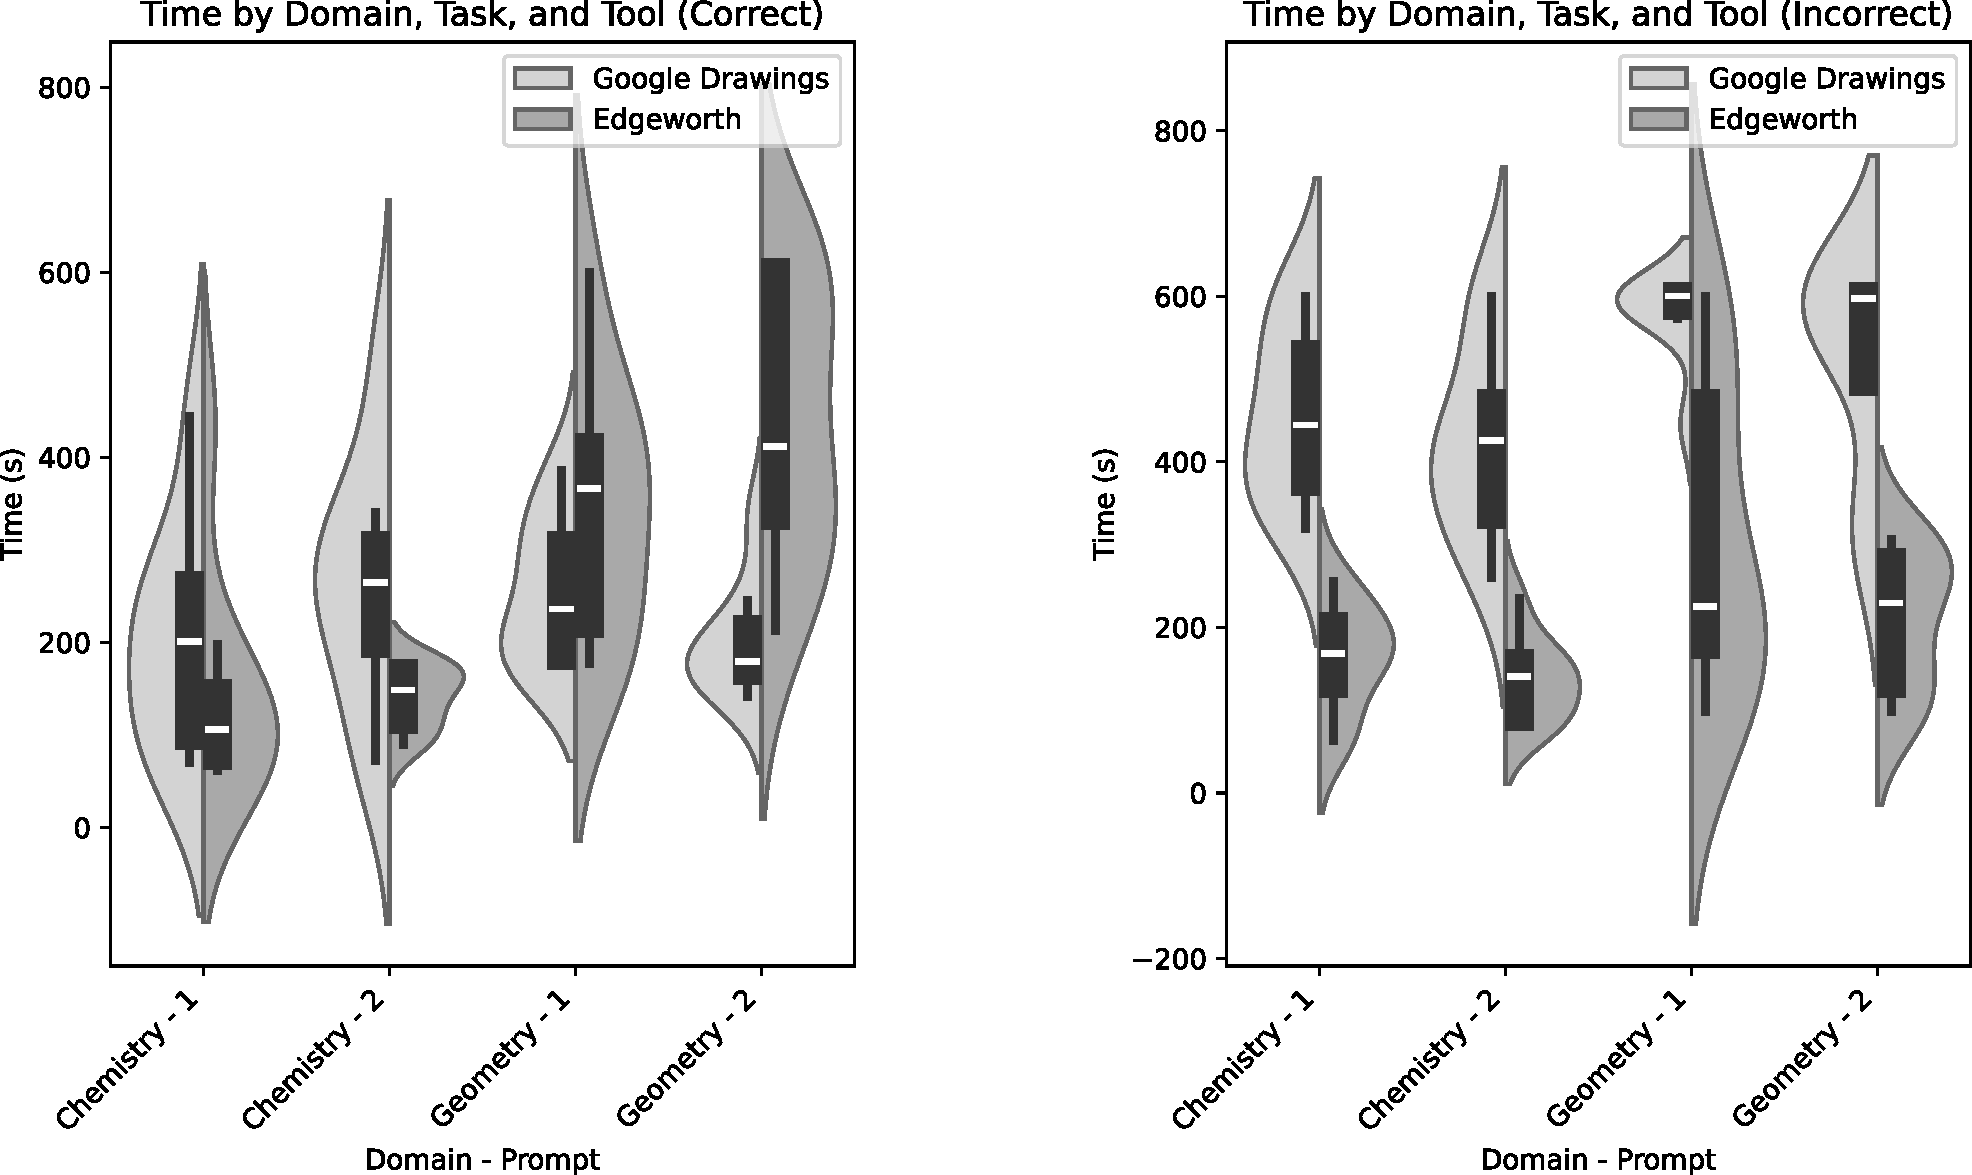
\includegraphics[width=\linewidth]{assets/edgeworth-eval/timing-violin.pdf}
    \caption{Violin plots showing the distribution of time-on-task for both correct (\textbf{Left}) and incorrect (\textbf{Right)} segments of tasks. The shape of the violins represents a smoothed approximation of the data distribution, with wider sections representing higher density. The embedded box plots within the violins show the median (white line) and inter-quartile range (thick black bar), with the whiskers (thin black lines) extending to the data range.}
    \label{fig:timing-violin}
\end{figure}


For the incorrect segments, the analysis revealed significant differences in task completion times between the tools used, visualized in \cref{fig:timing-violin} (right). In the chemistry domain, participants completed tasks significantly faster (almost 3 times faster) using \Edgeworth (\textit{M} = 150.13s, \textit{SD} = 59.15s) compared to Google Drawings (\textit{M} = 440.63s, \textit{SD} = 113.04s), as indicated by the significant main effect of tool, $F(1, 7) = 53.33, p = 0.0002$. There was no significant effect of the task itself, $F(1, 7) = 1.29, p = 0.293$, suggesting that the difficulty of the tasks was consistent regardless of the tool used. Similarly, in the geometry domain, participants also completed tasks significantly faster (similarly, almost 3 times faster) with \Edgeworth (\textit{M} = 257.25s, \textit{SD} = 139.55s) compared to Google Drawings (\textit{M} = 549.38s, \textit{SD} = 91.28s), with a significant effect of the tool, $F(1, 7) = 90.97, p < 0.0001$. There was a marginal effect of task, $F(1, 7) = 3.64, p = 0.098$, indicating a trend towards task differences that did not reach statistical significance. 

For the correct segments, the analysis showed mixed results on \Penrose's performance depending on the domain, illustrated in \cref{fig:timing-violin} (left). In the chemistry domain, participants completed tasks significantly faster using \Penrose (\textit{M} = 144.19s, \textit{SD} = 79.22s) compared to Google Drawings (\textit{M} = 231.81s, \textit{SD} = 129.78s), as indicated by the significant main effect of tool, $F(1, 7) = 6.65, p = 0.037$. There was no significant effect of the task itself, $F(1, 7) = 0.99, p = 0.353$. In the geometry domain, however, Google Drawings outperformed \Penrose, with participants completing tasks faster using Google Drawings (\textit{M} = 228.5s, \textit{SD} = 71.74s) compared to \Penrose (\textit{M} = 390.94s, \textit{SD} = 149.74s), as indicated by the significant main effect of tool, $F(1, 7) = 15.95, p = 0.005$. Again, there was no significant effect of the task itself, $F(1, 7) = 0.28, p = 0.611$.

% survey

In the per-task survey, summarized in \cref{tab:edgeworth-user-study-survey}, participants provided feedback on the tasks across two domains and both tools. For the chemistry tasks, \Edgeworth was rated highly across all survey items, with participants expressing a strong likelihood of using the problems in their classes (\textit{M} = 4.19), finding them pedagogically useful (\textit{M} = 4.25), and rating the visual quality of the diagrams as excellent (\textit{M} = 4.50). In contrast, Google Drawings received lower ratings in chemistry, particularly in terms of visual quality (\textit{M} = 2.81). In the geometry domain, \Edgeworth also was rated well, with participants finding it useful (\textit{M} = 4.06) and visually acceptable (\textit{M} = 3.38), although the ratings were slightly lower compared to chemistry. Google Drawings in geometry was rated lower across all dimensions, with middling scores for usefulness (\textit{M} = 3.50) and visual quality (\textit{M} = 3.44). Overall, \Edgeworth consistently out-rates Google Drawings, particularly in terms of the visual quality of the diagrams and pedagogical usefulness, especially in the chemistry tasks.

% MANOVA

We conducted a Multivariate Analysis of Variance (MANOVA) on the survey data to quantitatively assess the impact of the tool (\Edgeworth{} vs. Google Drawings) and the domain (chemistry vs. geometry) on three dependent variables corresponding to the survey questions. The results showed a significant effect of the tool on the combined dependent variables, with Wilks' lambda indicating that the choice of tool had a statistically significant influence on the survey responses, $F(3, 59) = 3.3995$, $p = 0.0235$. The domain (chemistry vs. geometry) did not have a significant effect on the combined dependent variables, $F(3, 59) = 0.7550$, $p = 0.5239$. A significant intercept observed in the analysis, $F(3, 59) = 217.9321$, $p < 0.0001$, suggests that the overall mean response across all groups was significantly different from zero, indicating that participants generally provided positive ratings across all survey items. In summary, \Edgeworth{} was perceived more favorably across the three survey questions compared to Google Drawings.


\begin{table}[t]
\centering
\begin{tabular}{l|l|l|l|l}
\hline
\textbf{Domain} & \textbf{Tool} & \textbf{Would Use} & \textbf{Useful} & \textbf{High Quality} \\ \hline
\multirow{2}{*}{\centering Chemistry} 
    & \Edgeworth
    & \progressbar{4.19} 4.19 & \progressbar{4.25} 4.25 & \progressbar{4.50} 4.50 \\ \cline{2-5}
    & Google Drawings 
    & \progressbar{3.63} 3.63 & \progressbar{3.94} 3.94 & \progressbar{2.81} 2.81 \\ \hline

\multirow{2}{*}{\centering Geometry} 
    & \Edgeworth 
    & \progressbar{3.94} 3.94 & \progressbar{4.06} 4.06 & \progressbar{3.38} 3.38 \\ \cline{2-5}
    & Google Drawings 
    & \progressbar{3.38} 3.38 & \progressbar{3.50} 3.50 & \progressbar{3.44} 3.44 \\ \hline
\end{tabular}
\caption{Survey responses for chemistry and geometry tasks using \Edgeworth and Google Drawings. Higher numbers (visualized in green hue) indicates positive responses and lower numbers (yellow and red hue) negative responses.}
\label{tab:edgeworth-user-study-survey}
\end{table}

\subsection{Discussion}

The results show a trade-off between the time taken to create correct diagrams using \Penrose and the efficiency of generating incorrect variations using \Edgeworth. Participants might spend more time on the initial correct diagram using \Penrose, but are significantly and consistently faster at making incorrect diagrams using \Edgeworth than Google Drawings. On average, participants were 3--4$\times$ faster using \Edgeworth. In geometry, the initial correct diagram took more time with \Penrose ($390.94$s per diagram versus $228.50$s with Google Drawings), but the time per incorrect diagram was much lower with \Edgeworth ($25.73$s) compared to Google Drawings ($100.90$s). 

The initial investment in the first \Substance program differs depending on the language complexity and layout consistency. Generally speaking, the \Penrose chemistry domain is simpler to learn than the \Penrose geometry domain. The chemistry domain has a simpler grammar consisting of atoms, bonds, and valance electrons. The layout for chemistry diagrams is also more stable and consistent. In contrast, the \Penrose geometry domain includes many predicates among points, line segments, lines, rays, angles, and so on. The geometry \Style is also less polished than that of chemistry. We observed that participants were sometimes confused by bad layouts produced by \Penrose, and doubted the correctness of their \Substance programs. The timing data in the correct segment shows the difference: participants were $1.7\times$ faster to make the correct diagram using \Penrose on average in chemistry, but $1.7\times$ slower in geometry.


\section{Expert Walkthrough Demonstration and Feedback (\ref{rq:eco})}
\label{sec:expert-feedback}

The intended users of \Edgeworth are educators who create problems. These users are very important to the education system since other teachers make use of their problems. Therefore, we recruited educators who created visual practice problems in multiple domains and educational settings to evaluate ecological validity of \Edgeworth-generated problems (\ref{rq:eco}). While an expert survey may suffice for rating problem quality, we opted for walkthrough demonstration, based on prior research on evaluation methods by \citet{ledo_evaluation_2018}, to gather additional qualitative feedback on the value of having the toolkit in their day-to-day work.

\subsection{Participants and Procedure}
\label{sec:expert-procedure}

We recruited domain expert educators of chemistry, geometry, and graph theory. Experts were invited based on their extensive teaching experience in the domain and past experience in \emph{authoring} diagrammatic content. In contrast to the criteria in the formative study (\cref{sec:edgeworth-formative}), this study selected participants based on their domain-specific expertise in authoring problems. Recruited educators came from a wide range of institutions, including Massive Open Online Courses (MOOC) platforms, liberal arts colleges, community colleges, research universities, and secondary schools. The average teaching experience among the 9 expert educators (E1–E9) was 10.33 years, with a standard deviation of 8.39 years, highlighting a broad range of teaching experience. One of the participants is the original author of the chemistry problems reproduced in the translation problem dataset (\cref{sec:edgeworth-case-studies}).
\cref{tab:demographics} summarizes the demographic information for 9 expert educators (E1--9) who participated in the study. 

\begin{table}
    \centering
    \begin{tabular}{l|l|r|l}
        \textbf{ID} & \textbf{Occupation} & \textbf{Years of Experience} & \textbf{Domain(s)}    \\
        \hline
        E1 & MOOC Course Designer       &  7 & Chemistry           \\ 
        E2 & Liberal Arts College Professor &  4 & Chemistry, Geometry \\
        E3 & Community College Professor    & 30 & Chemistry           \\
        E4 & Liberal Arts College Professor & 11 & Graphs              \\
        E5 & Research University Professor  & 17 & Graphs              \\
        E6 & Research University Professor  &  5 & Graphs              \\
        E7 & Middle School Teacher      &  5 & Geometry            \\
        E8 & Undergraduate Teaching Assistant &  3 & Geometry, Graphs    \\
        E9 & High School Teacher        & 11 & Geometry, Graphs    \\
    \end{tabular}

    \caption{Demographics of walkthrough demonstration participants.}
    % \Description{A table showing the demographics of participants in walkthrough demonstration sessions. It has four columns labeled: ID, Occupation, Teaching Experience, and Domain(s). The entries are: E1 as a MOOC Course Designer with 7 years in Chemistry, E2 as a Professor at a Liberal Arts College with 4 years in Chemistry and Geometry, E3 as a Professor at a Community College with 30 years in Chemistry, E4 as a Professor at a Liberal Arts College with 11 years in Graphs, E5 as a Professor at a Research University with 17 years in Graphs, E6 as a Professor at a Research University with 5 years in Graphs, E7 as a Middle School Teacher with 5 years in Geometry, and E8 as an Elementary School Tutor and Undergraduate TA with 3 years in Geometry and Graphs.}
    \label{tab:demographics}
\end{table}

Each expert participated in a 60- to 90-minute session via video conferencing, which was recorded with their consent. At the start of each session, we demonstrated the workflow of \Edgeworth end-to-end, as described in \cref{sec:edgeworth-workflow}, on one problem outside of the expert's domain. For the remainder of the session, we asked the expert to assemble problems from the \Edgeworth output of two to four problem prompts randomly sampled from the translation problem dataset (\cref{sec:edgeworth-case-studies}) in their domain. Per prompt, the expert rated 10 diagram variations based on the categories described in \cref{sec:reliability-method}. In addition, we asked participants to provide more granular feedback on diagram quality. After rating the diagram variations, they were asked to pick diagrams to assemble a four-choice diagrammatic translation problem. After the problem was assembled and shown on the interface, we asked (1) if they would use the problem in their instruction and (2) how they would author the diagram using their own workflow. The full study protocols for both the chemistry and geometry group are included in \cref{app:edgeworth-user-study-protocol}.

% \subsection{Existing Problem Authoring and Diagramming Processes}

% % thesis: diagramming is a design problem and experts 

% % use of diagrams
% Experts report a wide range of diagram use such as problem sets (E1, E3, E4, \hl{E9}), worked examples (E2--\hl{9}), tests (E1, E2), and in-class activities (E2, E7). Most experts favor multiple-choice translation problems, especially when \quotei{the class size grows} (E2). A few experts favor free-response questions for better feedback to students but noted the scalability problem with them (E2, E3, E7, \hl{E9}). For instance, E3 pointed out that they \quotei{can't monitor how 75 students are drawing a Lewis structure.} 

% % diagram is hard
% To make diagrams, experts used tools such as Microsoft Powerpoint (E1, E3), LaTeX (E4, E5, E6, E8), InkScape~\cite{bah2011inkscape} (E4), Geogebra~\cite{geogebra5} (E2, E7), \hl{and Desmos}~\cite{desmos} (E9). Similar to prior studies on diagramming tools~\cite{naturalDiagramming}, they reported barriers to using these tools that led to \quotei{painful} (E1, E2, E5, E6, E8) diagramming processes. As a result, if possible, they often fell back to hand-drawn diagrams because they \quotei{take less time} (E1, E4, E6), but E5 noted drawing skill is \quotei{one of the talents I did not have and I wish I did.} High-quality diagrams also take significant crafting to get right. For example, E4 would still \quotei{easily spend a day} on a figure because \quotei{if I start trying to make a perfect vector graphics version of it, it's inevitable. We just go down a rabbit hole of trying to make it look nicer and nicer.} 

\subsection{Ecological Validity of Generated Problems}

Overall, experts were happy with the problems they assembled with \Edgeworth-generated diagrams. Experts (E1--9) indicated that they would use all of the problems they created using \Edgeworth in their coursework. Other experts said they would use \Edgeworth-generated problems \quotei{early in the learning process} (E3) and \quotei{as a warm up exercise at the start of the next lecture} (E4). In addition, expert said these problems could be used to review previously introduced concepts. For example, E3 found the diagram variations that break the octet rule to be useful for \quotei{after you've also introduced expanded octet or non-octet-rule things.} Experts plan to use \Edgeworth-generated problem to \quotei{focus on things that students struggle with} (E3) and when introducing concepts that are \quotei{all about visualization} (E5) such as planarity of graphs. E7 asked to see all problems we gathered in the translation problem dataset (\cref{sec:edgeworth-case-studies}) and was excited to them in their class because they were \quotei{going to be covering everything [on the list].} In addition to just asking students to select correct diagrams, E3 also pointed out that by prompting students to \quotei{tell me what is wrong rather than just which is the correct one,} the problem can be used to \quotei{dive deeper.} Similarly, E4 proposed to use \Edgeworth problems as \quotei{an interactive warm-up for reviewing the last lecture, where students vote on and explain why a diagram is correct.} E7 even plans to use \Edgeworth as \quotei{a creative instead of assessment piece} and \quotei{have the students be the teacher \dots{} playing this role more, they get better at tests, because they understand what the test makers are doing.} 

\subsection{Expert Feedback}

\subsubsection{Experts provided positive qualitative feedback on \Edgeworth}
% fast and good
Experts reacted positively to \Edgeworth. They found \Edgeworth to be a \quotei{perfect fit} (E1, E6, E8) for generating multiple-choice problems, especially \quotei{low-stake} (E2, E3, E5, E6, E8, E9) quizzes that \quotei{incentivize [students] to keep up with the class} (E8). Experts said the automatic layout of \Edgeworth \quotei{draws things really fast} (E5), \quotei{saves you the time of drawing multiple structures} (E3), and produces \quotei{beautiful} (E4, E7) diagrams. Comparing with their existing tools, \Edgeworth is a \quotei{nice time-saver} (E3) and the translation problems they authored during the session would take an \quotei{enormous amount of work} (E4), \quotei{infinitely longer than this took} (E6).

Notably, experts pointed out that \Edgeworth aids creativity by promoting \quotei{recognition over recall} (E6). Specifically, \Edgeworth helps with \quotei{the thinking about how to come up with the graphs} and simplifies the diagram layout such that \quotei{you just generate some mutations that you click refresh until it looks nice} (E6). E2 liked that \quotei{it can come up with different possibilities than the ones that would be immediately apparent to me.} 

In addition, experts commented that \Edgeworth can enable them to give students more practice. For instance, E4 noted that \quotei{there's a feedback loop where \dots{} if I had a really good tool for generating nice multi-choice questions, then I could envision doing that much more frequently.}  

Importantly, in the context of student authoring problems themselves, E7 thinks that lowering the barrier of problem authoring help students \quotei{feel they have ownership in their learning as well as sharing their ownership with other students in the class.}

\subsubsection{Experts used visual selection to express diverse standards on diagram quality}
\label{sec:edgeworth-expert-standards}

When rating diagram mutants, experts agreed with diagram ratings of \cref{sec:reliability-eval}, but expressed unique standards for selecting answer choices (\cref{sec:expert-procedure}). Since experts had different standards, they selected different diagrams to assemble problems. This suggests \Edgeworth's use of visual selection met experts' needs.

One group of experts (E2, E4, E6, E7, E8, E9) preferred to maintain a balanced mix of answer choices, \quotei{at least one that's obviously correct, at least one that's obviously incorrect, and then \dots{} two where you have to think about that a little bit} (E6). One rationale was to \quotei{make sure [the problem] is challenging enough, but also has some things that are accessible to students that haven't completely mastered the material} (E4). Another was to teach \quotei{the process of elimination} (E7, E9). Another group of experts (E1, E3, E5) had much higher standards for including a mutant in a multiple-choice problem. For example, E1 preferred problems to contain one correct answer and multiple distractor options that are \quotei{less obvious} such that students won't \quotei{pattern match without looking at the details.}

On a problem that E2 accepted 7 out of 10 mutants as good incorrect options, E3 discarded 8 out of 10 because they \quotei{violated the octet rule in egregious or blatantly egregious way.} However, E3 said whether the octet rule can be broken depends on \quotei{where students are in the course.}

The difference of standards is highly individual. From E2's knowledge of \quotei{colleagues [who] only give difficult distractors} and \quotei{certain profs [who] are legendary for having really hard multiple choice,} they guessed that harder problems \quotei{motivate the students to try harder,} but also pointed out that it \quotei{only works for certain students in my experience.} E3 stated that their choice in diagrams \quotei{hinges upon my perception of whether students will automatically disqualify something,} which they admitted is \quotei{a certain premise or bias.}  In E3's words: \quotei{Wow, it's really tough to \dots{} completely take off the instructor hat.} 

This comment reflects the concept of \textit{expert blind spot} in learning sciences literature, where experts fail to \quotei{understand the processes of novices who are struggling to understand new ideas during their constructive learning process} ~\cite{expertBlindspot}.

\subsubsection{Experts selected isomorphic diagrams to build conceptual understanding}
\label{sec:isomorphic-diagrams}

\Edgeworth sometimes produces isomorphic diagrams, \ie diagrams with identical content but different layouts. These diagrams occur when \Edgeworth's mutations have no net impact on the example diagram, \eg the mutator removes an edge from a graph and adds it back. Surprisingly, experts found value in these isomorphic diagrams. 
In their geometry course, E2 said that their textbook's diagrams \quotei{get drawn the same way over and over again. And some students get stuck into thinking that the concept is only communicated when the diagram is drawn [exactly] that way.} When assembling a problem about the $HCN$ molecule, E3 compared two isomorphic variations, and picked one over another because \quotei{it's drawn the opposite \dots which is interesting and I think students are going to get it wrong.}  Similarly, E1 finds isomorphic diagrams to be useful for \quotei{molecules with resonance structures.} 
% However, for simpler molecules, E1 cautioned that might mislead students to think that \quotei{they are different structures when they really are the same.} 
E5 found isomorphic planar graphs to be particularly useful because students find them \quotei{painstaking to visualize when they just started.} E5 planned to use \Edgeworth to \quotei{draw a graph that doesn't look like it could be planar first, but then untangle it to show that the graph is actually planar.}

% \cref{sec:problem-generation} further discusses this possibility in the context of existing template-based problem generation tools.



\section{Limitations of the Studies}

We discuss some limitations to the studies presented in this chapter. 

% \subsection{Sample Size and Generalizability}
% The sample sizes in the user study and expert walkthrough were relatively small, with only 16 participants in the user study and 9 expert educators in the walkthrough sessions. This limited number of participants may not fully represent the broader population of educators or the variety of instructional contexts in which \Edgeworth might be applied. Consequently, the generalizability of the findings to other domains, educational settings, or different types of diagrammatic problems is limited.

\subsection{Ecological Validity}

The studies primarily focused on specific instructional domains, including chemistry, geometry, and graph theory. While these domains were chosen from the translation problem dataset, the studies are limited by the scope of the dataset itself. The performance and effectiveness of \Edgeworth might vary when applied to other fields that require different types of visual problem representations, which were not explored in this research.

Although the expert walkthroughs provided valuable feedback on the ecological validity of \Edgeworth-generated problems, the artificial nature of the study environment might not fully capture the complexities and constraints of real-world educational settings. The experts' feedback were based on hypothetical scenarios and short-term interactions with the tool, which may not fully reflect the challenges and demands of long-term usage in a classroom or curriculum development context.

\subsection{Tool}
\label{sec:edgeworth-limitations}

Participants in the user study were provided with brief tutorials on using \Edgeworth and Google Drawings, which may not have been sufficient for them to become fully proficient with these tools. The learning curve associated with \Penrose and \Edgeworth, especially their unique approach to generating diagrammatic problems, might have influenced the results, particularly in the efficiency evaluation. Participants with more extensive experience or training in using either tool might exhibit different levels of efficiency and satisfaction than those observed in the study.

% \subsection{Focus on Multiple-Choice Problems}
% The studies were designed around the generation and evaluation of multiple-choice problems, which, while useful in many educational contexts, represent only a subset of the types of problems educators might want to create. Other problem types such as open-ended questions or interactive exercises, were not explored.

% \subsection{Technical Constraints and Evolution}

Both \Penrose and \Edgeworth are still under development, and the studies were conducted on particular versions of them. As they evolve, with potential updates and improvements, the findings presented here might become outdated. Future research would need to re-evaluate the tool's performance and usability in light of new changes. \cref{sec:penrose-limitations} and \cref{sec:limitations} discuss the specifics of \Penrose's and \Edgeworth's system limitations.

\subsection{Authoring Speed vs. Problem Quality}

\begin{figure}[t]
    \centering
    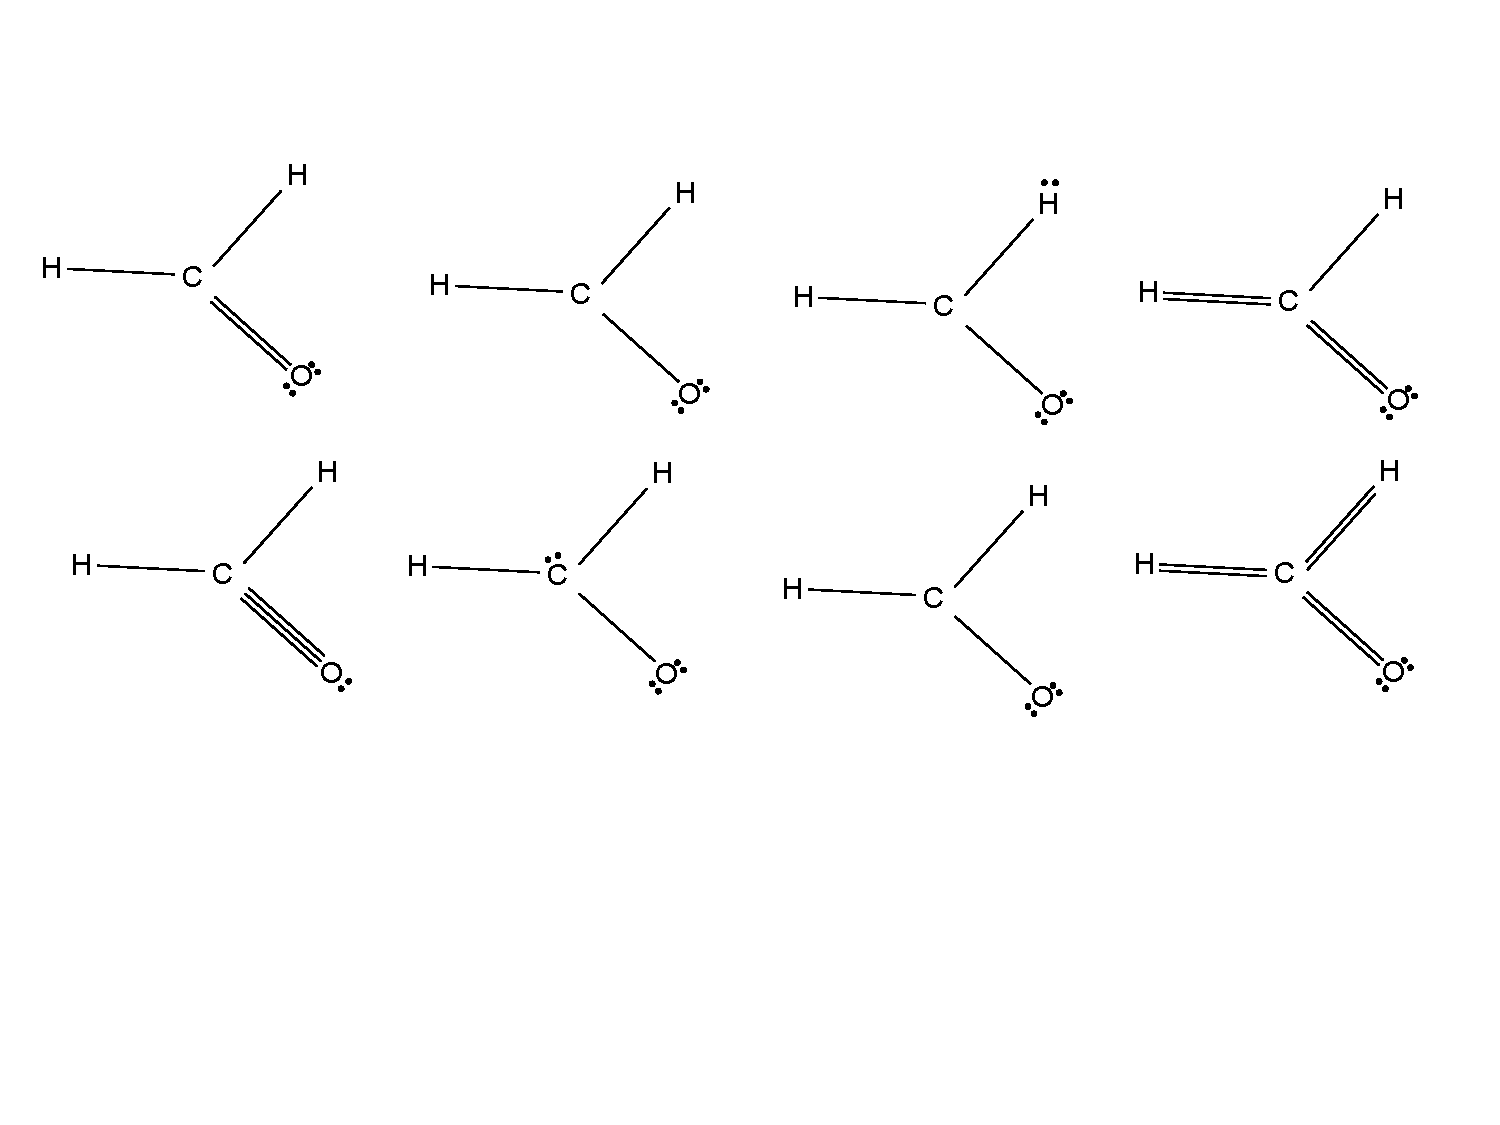
\includegraphics[width=\linewidth]{assets/edgeworth-eval/p4-drawings.pdf}
    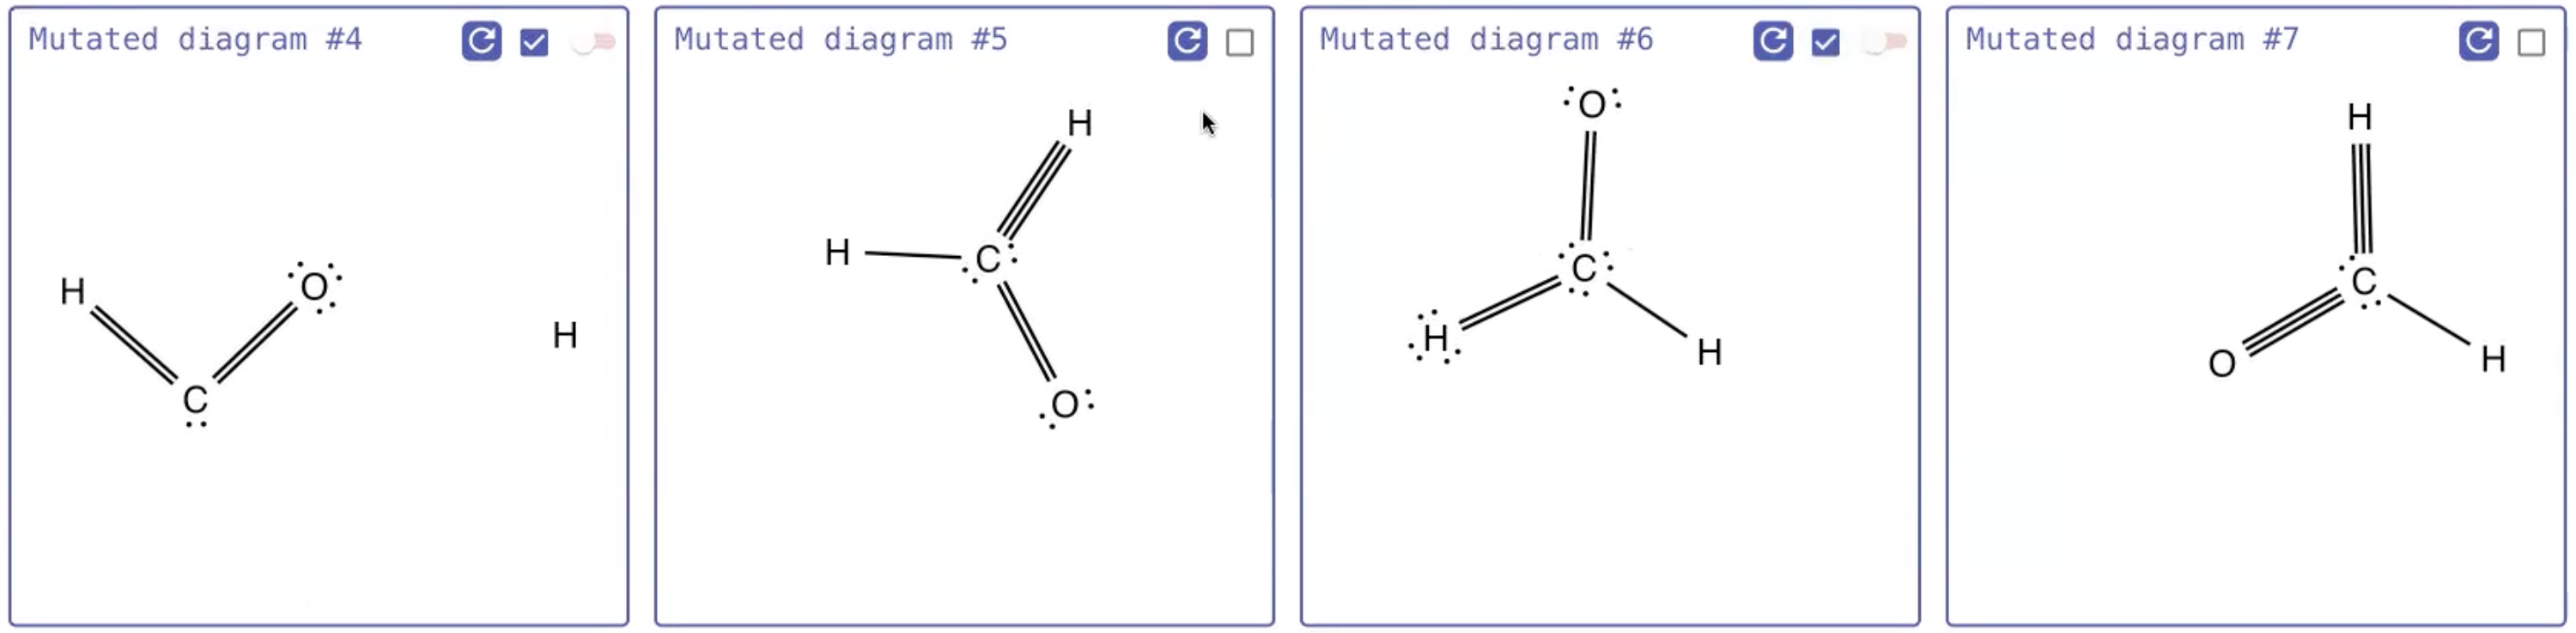
\includegraphics[width=\linewidth]{assets/edgeworth-eval/p4-edgeworth.png}
    \caption{Screenshots of Google Drawings \figloc{(top)} and \Edgeworth selections \figloc{(bottom)} of diagrams by P4 of the user study (\cref{sec:edgeworth-user-study}). They are instances of ``shortcuts'' participants took when using both tools, avoiding large layout edits \figloc{(top)} in Google Drawings and selecting counterexamples seemingly at random in \Edgeworth \figloc{(bottom)}. }
    \label{fig:edgeworth-user-study-shortcuts}
\end{figure}


Participants in the user study described in \cref{sec:edgeworth-user-study} were not screened for their prior experience nor expertise in diagrammatic problem authoring. In fact, a majority of them are undergraduate students. Therefore, their judgment of what makes a good problem (or lack thereof) might influence the task performance data reported in \cref{sec:edgeworth-user-study}. Theoretically, to get through the tasks, participants could pick incorrect diagrams at random using \Edgeworth, or make minimal edits to the correct diagram to get alternatives using Google Drawings. To address this limitation of the user study, we conducted  expert demonstration walkthroughs \cref{sec:expert-feedback} to gain a deeper understanding of the ecological validity of \Edgeworth-generated problems.

During the user study, we did in fact observe participants taking shortcuts in both conditions. Here we show some examples of them and contrast them with the experts' opinions. For instance, \cref{fig:edgeworth-user-study-shortcuts} (top) shows P4's pattern of making small edits to the correct diagram to quickly produce incorrect diagrams. These edits avoids moving many diagram components around while maintaining a good layout. The similar layouts of atoms and bonds contrast experts' feedback on isomorphic diagrams (\cref{sec:isomorphic-diagrams}, \eg \quotei{some students get stuck into thinking that the concept is only communicated when the diagram is drawn [exactly] that way.} by E2). As another example for \Edgeworth, \cref{fig:edgeworth-user-study-shortcuts} (bottom) shows two diagrams selected by a participant as suitable incorrect answers for chemistry prompt 1 (\textit{Which of the following diagrams shows the correct Lewis structure for \ensuremath{\mathrm{CH_2O}}?}) in \cref{fig:edgeworth-user-study-tasks}. Per their feedback in \cref{sec:edgeworth-expert-standards}, E3 would not accept ``Mutated Diagram \#6'' in the figure as a good incorrect options, because it \quotei{violated the octet rule in egregious or blatantly egregious way.}\footnote{The Carbon (C) atom in the diagram has 6 valance electrons, 2 double bonds, and one single bond, which is way beyond the expected 8 electrons and bonds combined per the octet rule.} Notably, as we discussed in \cref{sec:edgeworth-expert-standards}, experts did not agree on a single standard of high problem quality among themselves. 

Overall, while participants took shortcuts in both user study conditions, we do not know how much impact their quality standards have on the task performance. Importantly, there is not a single standard for ``good'' judgment of problem quality, as the expert demonstration walkthroughs showed a diversity of standards among experienced educators. Therefore, future research is needed to tease out (1) what is an acceptable quality standard for diagrammatic translation problems and (2) the effect of problem quality on authoring speed of diagrammatic problems. 

\section{Limitations of the \Edgeworth System}
\label{sec:limitations}

In this section, we further discuss some limitations of the \Edgeworth system in general.

\subsection{Numerical and textual variations}

\Edgeworth cannot produce numerical and textual variations like traditional problem generators~\cite{aleven_cognitive_2006, ASSISTment} do. It is, however, possible to build this functionality on top of \Edgeworth to produce further problem variations. 

\subsection{Usability of UI components}

The design presented in \cref{sec:edgeworth-system-design} focuses on generating diagram variations and selecting diagram mutants to create problems. We use the \Substance language and \Penrose's textual interface without modification. Any limitations of \Substance and its UI are inherited by \Edgeworth. We use standard Material UI elements\footnote{\url{https://mui.com/}} to allow users to configure \Edgeworth (\eg a standard text box for changing diagram variations in \cref{fig:edgeworth-interface}\uilabel{c}). While these components might be usable as-is, they are not designed explicitly for the problem authoring workflow. 

\subsection{New domains of instruction}
\label{sec:extension}

As shown in \cref{sec:edgeworth-mutation}, the design of the \Edgeworth mutator is domain-agnostic, as the mutation operators do not require any domain-specific knowledge to produce mutants. However, improving \Style requires domain expertise. Therefore, future \Edgeworth authors may not have the technical background or the time to invest in a new \Style program, which might prohibit them from using \Edgeworth if the domain is not well supported by the \Penrose ecosystem. However, as noted in \cref{chp:penrose}, the effort to build \Penrose stylesheets for new domains is only necessary once per domain and not once per diagram or problem.

\subsection{Mismatches with the author's intents} 

The \Edgeworth mutator can be sensitive to both the example diagram and the mutator configuration (\cref{sec:edgeworth-mutation}). For instance, a statement in the user-provided \Substance program might be particularly more suitable for mutations than others (perhaps because it contributes to the correctness of the problem.) Under- or over-specifying mutations in the configuration might lead to a pool of ``noisy'' diagrams. When these diagrams don't satisfy the needs of the author (\eg missing counterexamples that are important for an educational goal), the author can only generate another pool of mutants and hope to get better ones. For example, suppose an author would like to create translation problems that test students' knowledge of improper subsets, especially the fact that if $A \subseteq B$, $A = B$ is allowed. Using the \Edgeworth mutator, the author first creates a \Substance program:

\begin{center}
\begin{verbatim}
Set A, B, C
SubSet(B, A)
Subset(C, A)
\end{verbatim}
    
\end{center}

\begin{figure}
    \centering
    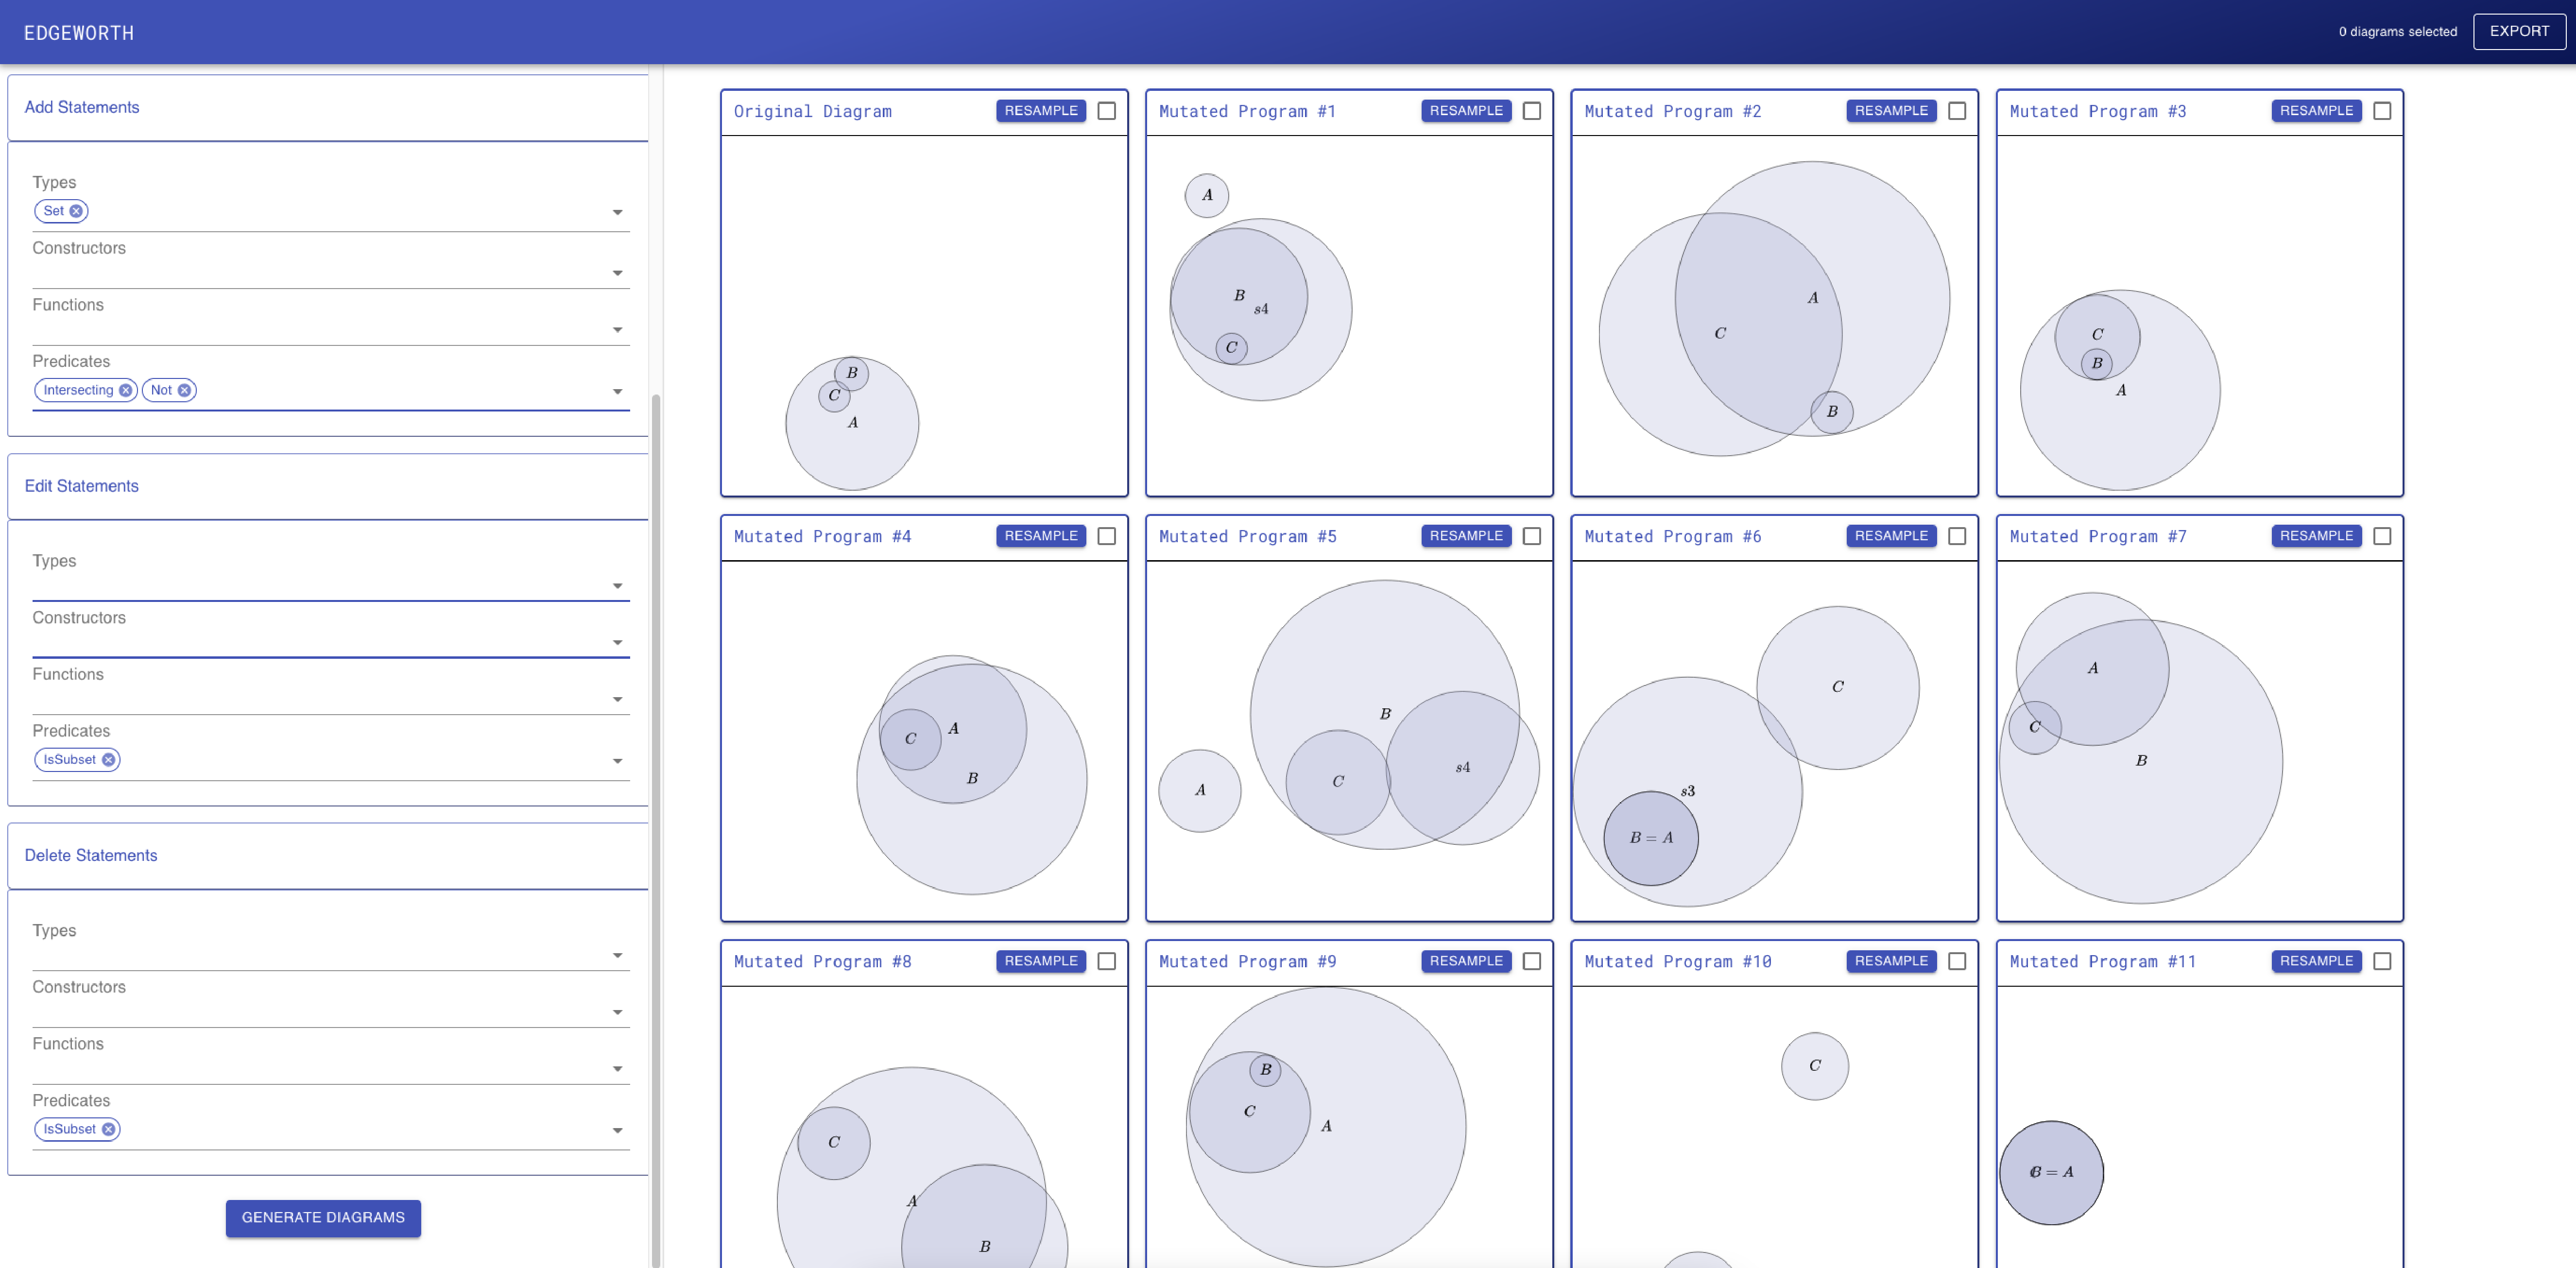
\includegraphics[width=\linewidth]{assets/appendix/edgeworth-bad-output.pdf}
    \caption{A screenshot of the \Edgeworth interface, after generating examples for a translation problem focusing on improper subsets. Because of randomness, the pool of mutant diagrams aren't suitable for this problem.}
    \label{fig:edgeworth-bad-output}
\end{figure}

The author then clicks ``Generate Diagrams.'' Ideally, \Edgeworth should generate a set of examples of the subset relations that include the edge cases of $A = B$, $A = C$, or $B = C$, and counterexamples of $B \not\subseteq A$ or $C \not\subseteq A$. 

However, the output from \Edgeworth seems too random (\cref{fig:edgeworth-bad-output}). There are acceptable counterexamples, but none of the diagrams include pedagogically useful cases such as:

\begin{center}
\begin{verbatim}
Set A, B, C
SubSet(B, A)
Subset(C, A)
Equal(B, C)
\end{verbatim}
\end{center}

In other words, the author cannot express their intent easily with the current version of \Edgeworth and may have trouble finding good mutants if they intend to create specific types of examples. We discuss the possibility of augmenting \Edgeworth with domain-specific knowledge, and allowing the user to express their pedagogical intents in \cref{sec:knowledge}


\section{Summary}

This chapter presents an evaluation of \Edgeworth through three studies focusing on its reliability, efficiency, and ecological validity. The research questions addressed are whether \Edgeworth can reliably generate translation problems with minimal variations (\ref{rq:mut}), if it enhances authoring efficiency compared to conventional tools (\ref{rq:eff}), and whether educators find the generated problems useful in real-world contexts (\ref{rq:eco}).

The first study (\cref{sec:reliability-eval}) assessed the reliability of \Edgeworth by analyzing 310 diagram variations across 31 problems. The results indicated that \Edgeworth successfully generated valid multiple-choice problems for most prompts within 10 diagram variations, demonstrating its reliability in producing consistent and usable outputs (\ref{rq:mut}).

The second study (\cref{sec:edgeworth-user-study}) compared the efficiency of authoring translation problems using \Edgeworth versus Google Drawings. The findings revealed that participants were significantly faster when using \Edgeworth (\ref{rq:eff}).

The final study (\cref{sec:expert-feedback}) involved expert educators who provided feedback on the ecological validity of \Edgeworth-generated problems. The educators found the problems to be pedagogically useful and expressed interest in using \Edgeworth in their instructional practices. Their feedback also emphasized \Edgeworth's potential to save time and enhance creativity in problem design (\ref{rq:eco}).

Overall, these studies demonstrate that \Edgeworth is a reliable and efficient tool for authoring educational problems, with strong support from educators for its application in diverse instructional contexts.







\chapter{Conclusion and Future Work}
\label{chp:conclusion}
\section{Summary of contributions}

This thesis makes several significant contributions to the study of diagramming, diagramming tools, and educational technology, including:

\begin{itemize}

    \item An interview study of the diagramming process, providing detailed insights into how experts across different domains create and use conceptual diagrams. This study documents how expert from a diverse set of domains author diagrams and identifies key challenges in existing diagramming tools (\cref{chp:interviews}).

    \item A natural diagramming framework that specifies four dimensions of diagramming tool design opportunity that seamlessly and naturally translate diagrammers’ high-level ideas to illustrative and effective diagrams (\cref{sec:natural-diagramming}).
    
    \item \Penrose, a novel system for creating diagrams from plain-text descriptions (\cref{chp:penrose}). \Penrose allows authors to encode domain-specific visual representations and automatically lays out diagrams, bridging the gap between abstract ideas and their visual representation.
    
    \item \Edgeworth, a tool built atop \Penrose, aimed at automating the generation of multiple-choice diagrammatic translation problems (\cref{chp:edgeworth}). 
    
    \item A dataset of translation problems that includes real-world diagrammatic problems in graph theory, chemistry, and Euclidean geometry (\cref{sec:edgeworth-case-studies}).
    
    \item Empirical evidence supporting the reliability, efficiency, and ecological validity of \Edgeworth in educational contexts (\cref{chp:edgeworth-eval}). 
    
\end{itemize}


\section{Future work}

We now discuss potential future directions for \Penrose, \Edgeworth, and diagramming tool research in general. 

\subsection{Composable visual representations}

Over the years of building diagrams using \Penrose and \Edgeworth, we have observed that visual representations in different domains often share common visual components and layout patterns. Further, common visual techniques are widely used in diagramming to convey domain-independent concepts, such as using varying opacity or line weight to highlight parts of a diagram, maintaining layout consistency across multiple diagrams to form a visual narrative, or using sliders or other widgets to drive real-time physical simulations in interactive webpages. It seems natural to separate out these common patterns into their own components, suggesting that \Penrose's existing reusability of visual representations in \Style{} does not provide sufficient flexibility for the needs of digital diagrammers.

In the current version of \Penrose{}, authors can reuse geometric and layout primitives to create new \Style{} programs, and users consume these programs by writing different \Substance{} programs with them. Each \Style{} program is standalone and self-contained, meaning that everything from the styling of points to the color palettes must be defined within that program. In practice, this means that common visual design patterns are copied and pasted between \Style{} files. Additionally, it is common for individual diagrams within a domain to have customized visual elements to draw focus or illustrate a concept. Currently, the only way to override the domain-wide visual style in \Penrose{} is by using workarounds that involve more copying/pasting code in \Style{}. These two limitations result in repetitive and lengthy programs that require high effort to edit and maintain, even for expert \Penrose{} users.

While code duplication and multiple versions of \Style{} may be manageable on a small scale, we envision building a broader ecosystem of diagrams and this requires more flexible reuse mechanisms. We suggest \textbf{composability} as the main design goal for improving \Penrose{}. The existing layout primitives are an example of composability: authors can reuse and \emph{combine} multiple primitives to form new layout problems. Looking forward, we plan to allow diagrammers to create \emph{modules} of visual components and layout patterns. Through this mechanism, an author can draw together multiple different modules they need for their own diagram. And these modules can themselves be composed from other modules: for instance, a module for visualizing complex analysis might make use of lower-level modules for visualizing a coordinate plane and plotting curves, but build on top of that with domain-specific visuals for singularities in holomorphic functions. In addition to user-defined modules, there are also opportunities to build domain-independent visual techniques, such as individual object-level highlighting or annotations, into our languages or as standard library modules.

We believe this composable approach will open up new possibilities for diagrammers to collaborate and create more flexible, reusable, and expressive visual representations. Going forward, we plan to survey existing compose mechanisms such as modules, type systems, and package ecosystems to inform our design for \Penrose.

% leverage research on common building blocks of and layout patterns in specific domains of diagramming, to construct a substrate for composable visual representations.

\subsection{Knowledge-infused problem variation}


% \begin{figure}[h]
%     \centering
%     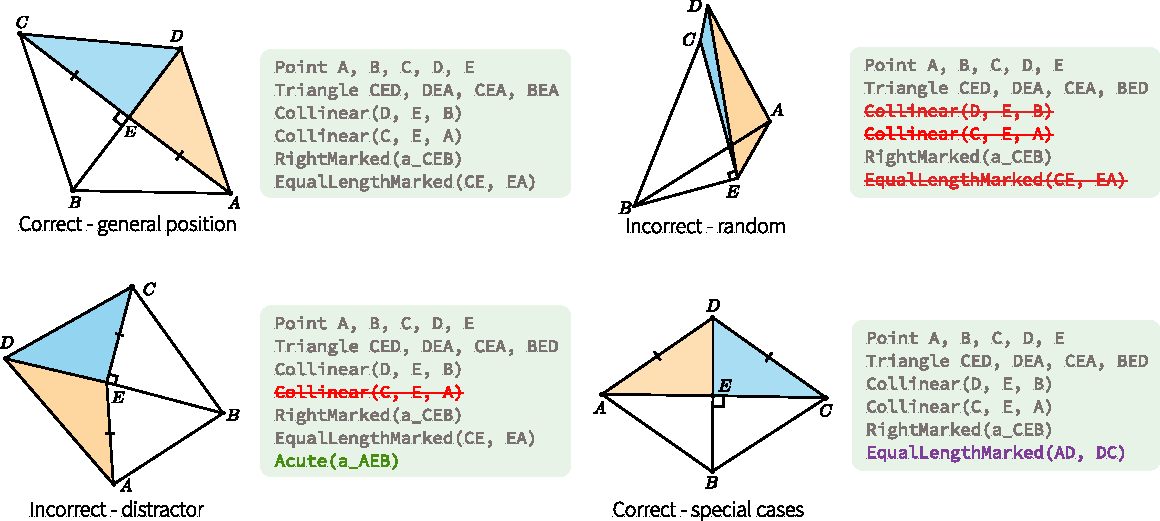
\includegraphics[width=\linewidth]{assets/chapter-3/answer-types.pdf}
%     \caption{Four example classes of problem options. \textbf{Top-left}: the example scenario, representing a general example. \textbf{Bottom-Left}: a counterexample that only slightly differs from the example scenario semantically. \textbf{Top-right}: a counterexample that differs significantly from the prompt. \textbf{Bottom-right}: an example instance that's a corner-case of the prompt.}
%     \label{fig:answer-types}
% \end{figure}

\Edgeworth provides a mixed-initiative~\cite{allen1999mixedinitiative} workflow: authors focus on specifying the content and the general direction of variations through the example scenario, while \Edgeworth fully automates the details of variation generation and layout. The evaluation studies presented in \cref{chp:edgeworth-eval} showed that this workflow improves authoring speed and can produce useful diagrams to educators already. In this section, we focus on the current state of \Edgeworth's outputs and propose future work for improving problem quality.

As discussed in \cref{sec:expert-feedback}, experts used terms like \quotei{obviously incorrect} (E6) and \quotei{less obvious} (E1) to characterize the quality of problem options in a multiple-choice translation problem. Based on their feedback, we divide these options into four categories: given a set of mathematical statements describing logical entities and their relationships, a diagram can be associated with them in one of the following ways:

\vspace{0.5em}
\begin{figure}[h]
\begin{minipage}[b]{0.48\linewidth}
$\bullet$ \textbf{Example}: the diagram represents the math statements, \ie all the statements hold true in the diagram. 
    \vspace{3pt}
    
$\bullet$ \textbf{Counterexample}: the diagram clearly violates the math statements, \ie one or more statements are false in the diagram.
    \vspace{3pt}
    
$\bullet$ \textbf{Positive edge case}: the diagram is an example of the math statements, but contains extraneous entities and/or more specialized relationships. 
    \vspace{3pt}
    
$\bullet$ \textbf{Negative edge case}: the diagram is a counterexample, but only requires a few changes to become an example.
\end{minipage}
\hfill
\begin{minipage}[b]{0.45\linewidth}
    \centering
    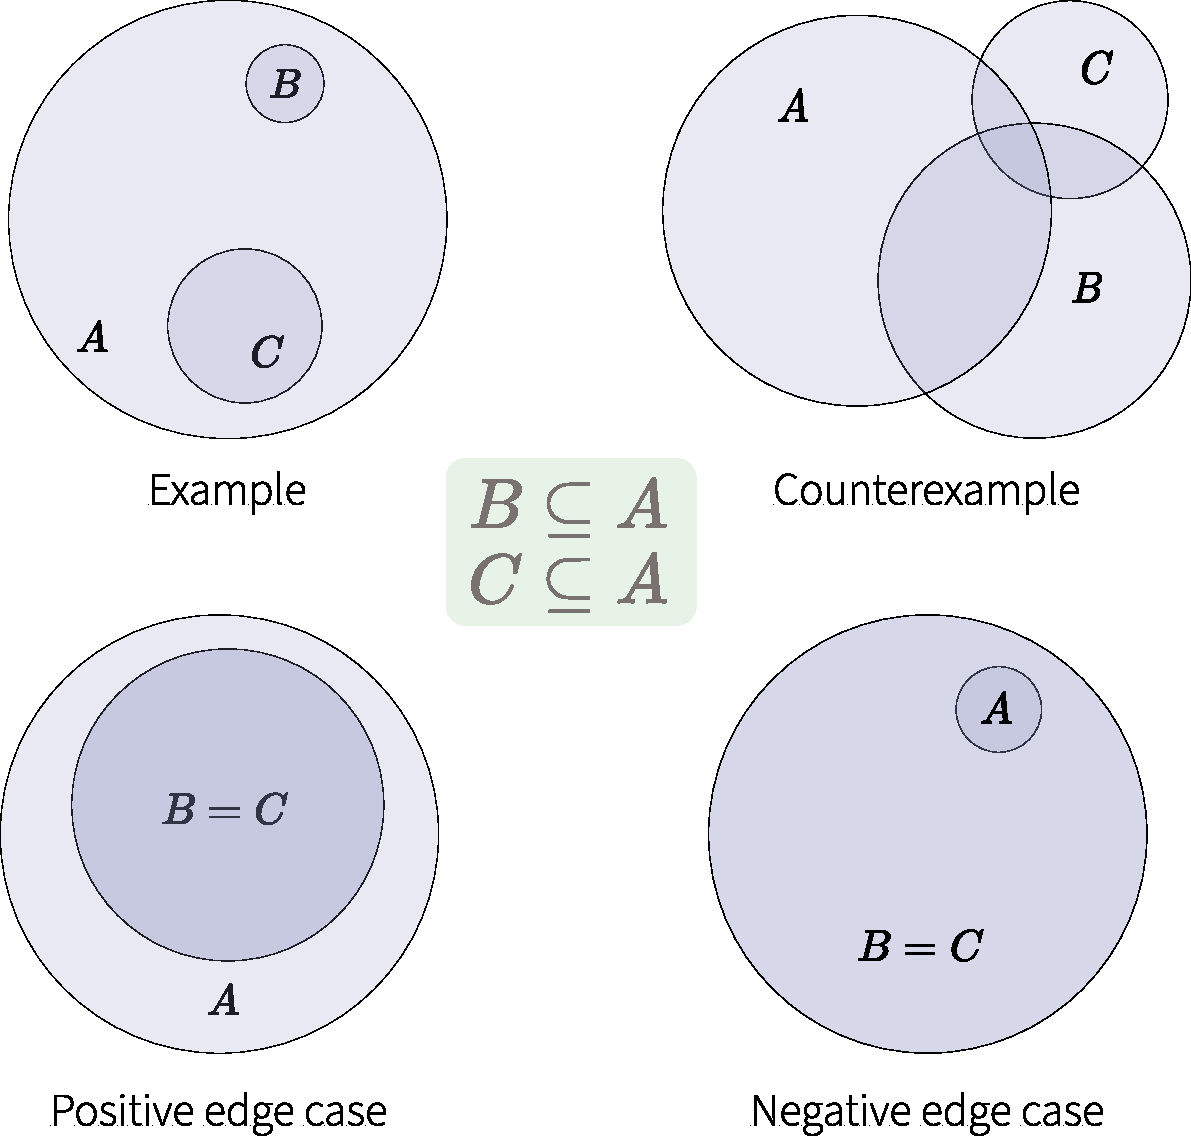
\includegraphics[width=\textwidth]{assets/appendix/definitions-examples.pdf}
\end{minipage}
\end{figure}

\begin{figure}
    \centering
    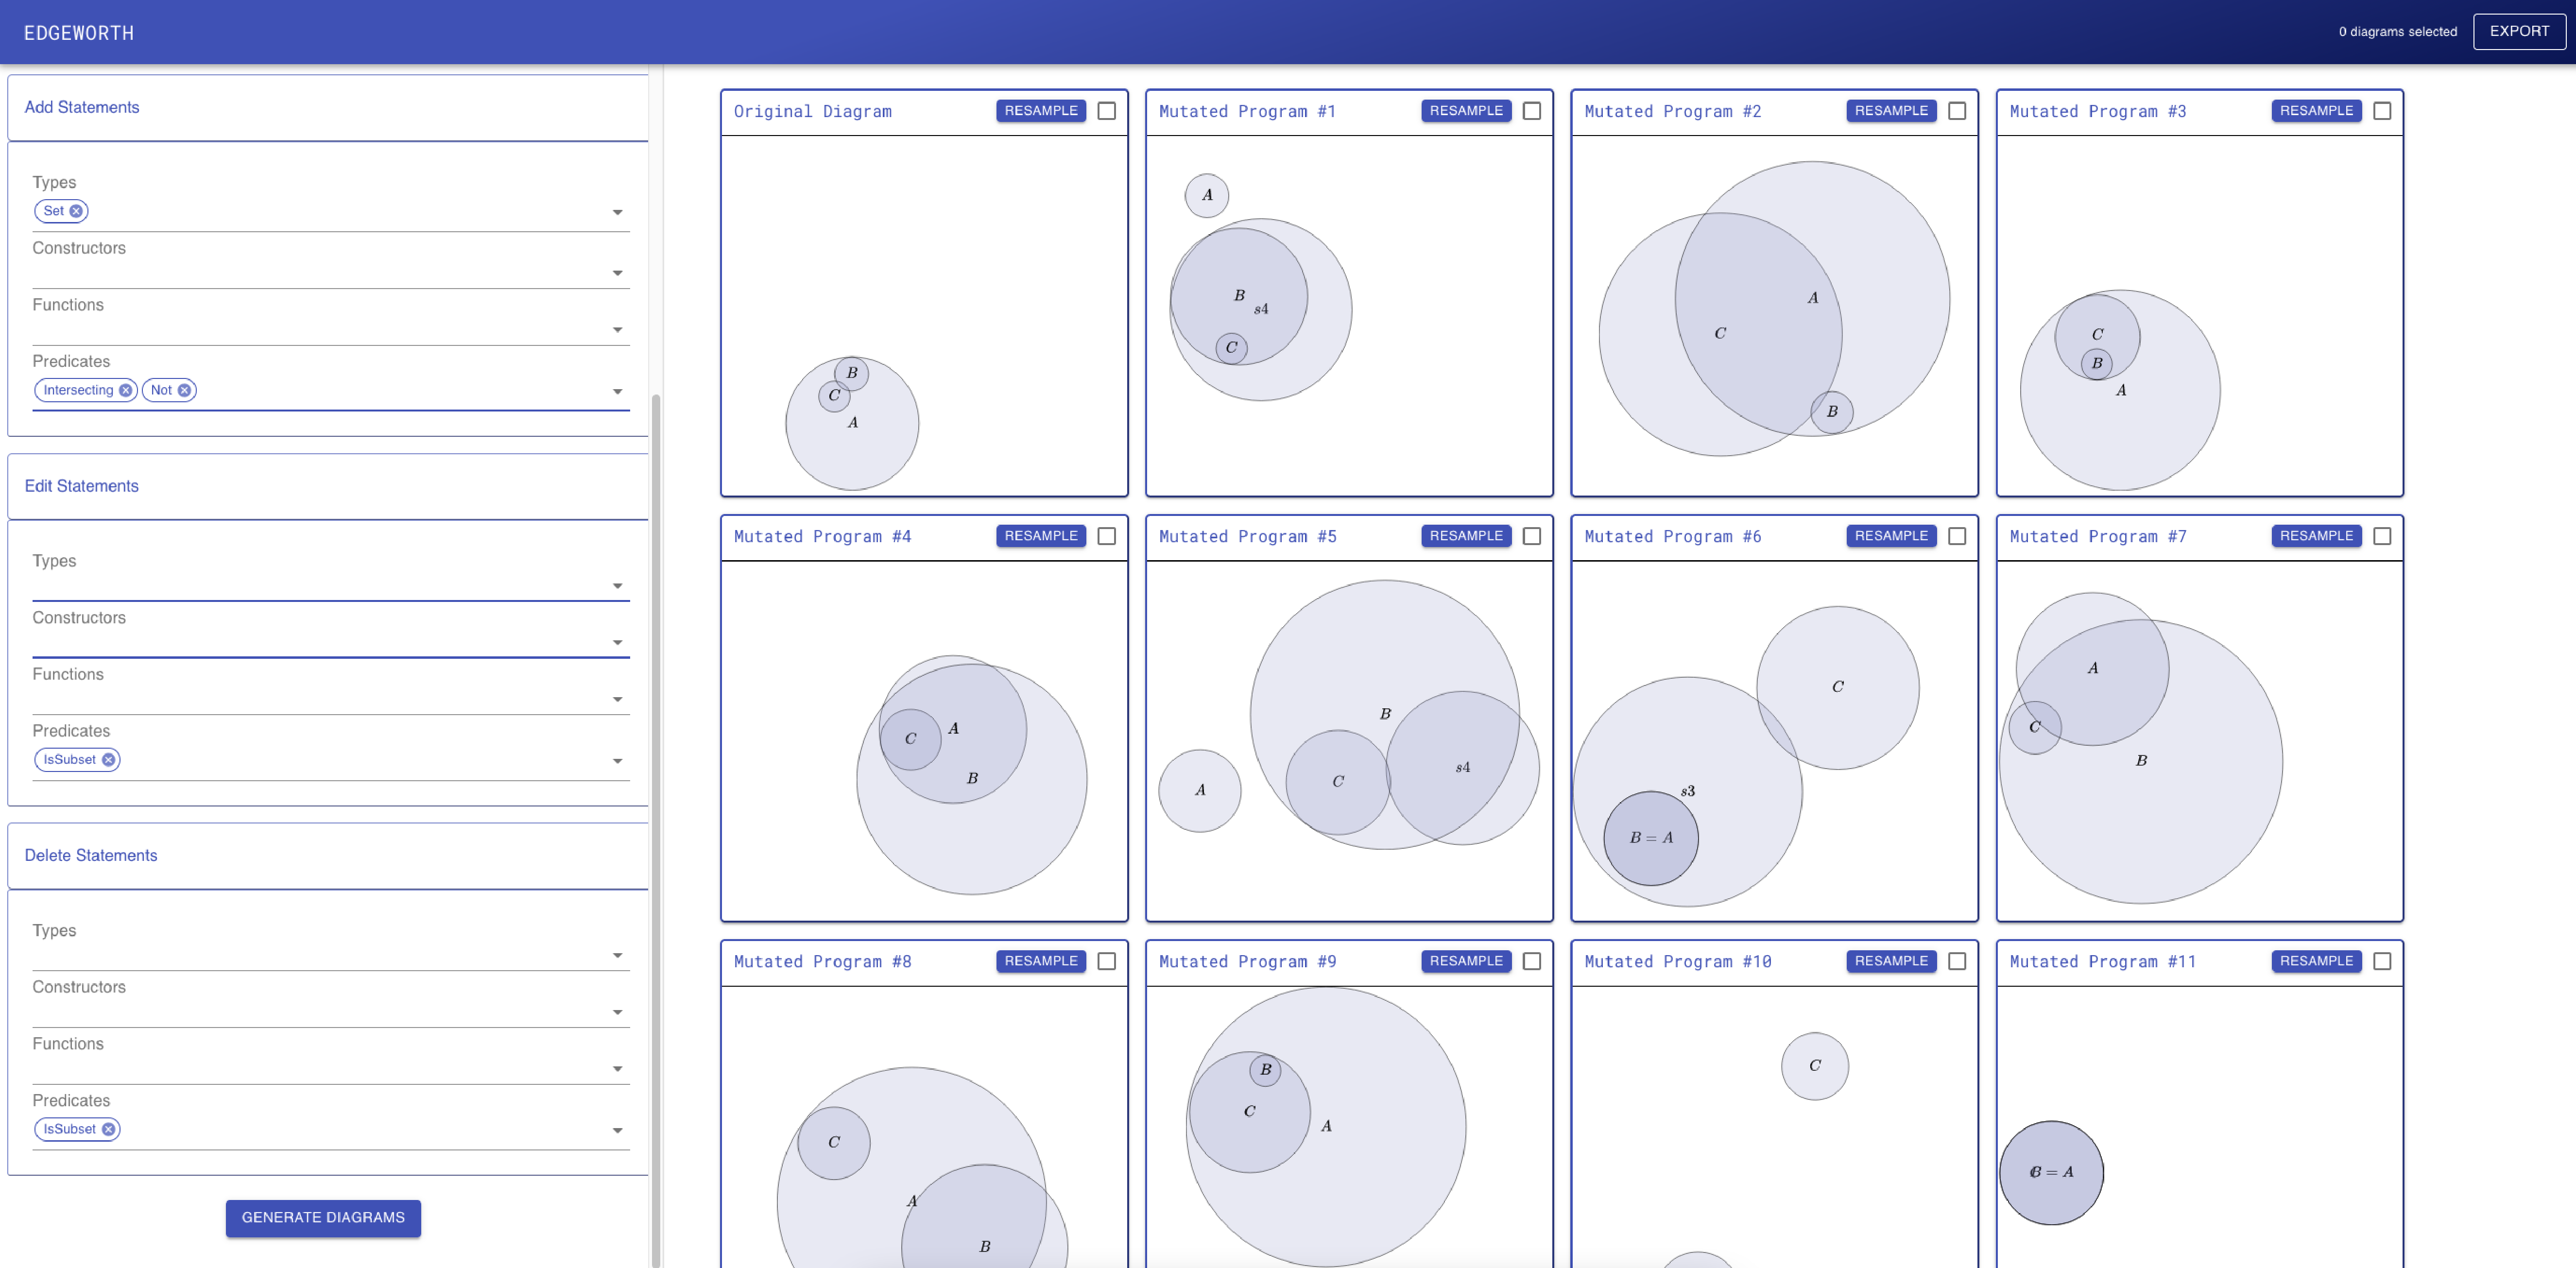
\includegraphics[width=\linewidth]{assets/appendix/edgeworth-bad-output.pdf}
    \caption{A screenshot of the \Edgeworth interface, after generating examples for a translation problem focusing on improper subsets. The first pool of mutants isn't suitable for this problem.}
    \label{fig:edgeworth-bad-output}
\end{figure}

Using \Edgeworth, the author creates an example scenario and \Edgeworth's mutator generates a set of diagrams. When these diagrams don't satisfy the needs of the author (\eg missing counterexamples that are important for an educational goal), the author can only generate more variations and hope to get better ones. For example, suppose an author would like to create problems that test students' knowledge of improper subsets, especially the fact that if $A \subseteq B$, $A = B$ is allowed. Using the \Edgeworth, the author first creates a \Substance program and clicks ``Generate Diagrams.'' 

\noindent\hspace*{\fill}
\begin{minipage}[c]{0.23\columnwidth}
\begin{mdframed}[style=SUBCode]
\begin{lstlisting}[language=Sub-SET,escapechar=@,numbers=none]
Set A, B, C
IsSubset(B, A)
IsSubset(C, A)
\end{lstlisting}
\end{mdframed}
\end{minipage}
\hspace*{\fill}

Ideally, \Edgeworth should generate a set of examples of the subset relations that include the edge cases of $A = B$, $A = C$, or $B = C$, and counterexamples of $B \not\subseteq A$ or $C \not\subseteq A$. However, those particular mutated programs are extremely unlikely to be generated by \Edgeworth. The default \Edgeworth output for this scenario is show in  \cref{fig:edgeworth-bad-output}. There are useful counterexamples, but none of the diagrams include edge cases such as:

\noindent\hspace*{\fill}
\begin{minipage}[c]{0.23\columnwidth}
\begin{mdframed}[style=SUBCode]
\begin{lstlisting}[language=Sub-SET,escapechar=@,numbers=none]
Set A, B, C
IsSubset(B, A)
IsSubset(C, A)
Equal(B, C)
\end{lstlisting}
\end{mdframed}
\end{minipage}
\hspace*{\fill}

\noindent In our experience, it is not uncommon for\Edgeworth to miss important edge cases. 

In future work, we propose to work with Large Language Models (LLMs) to generate high-quality edge cases. Since LLMs are trained on the text of the entire internet, they may contain enough knowledge to suggest pedagogically usefual positive and negative edge cases.

To turn these conceptual edge cases into diagrams, \Penrose{} needs \Substance programs. Therefore, we will first test LLMs capability to generate  \Substance programs.

Consider the case of a teacher authoring the example scenario (\cref{sec:create-scenario}): imagine the teacher specifying the diagram in natural language and an augmented version of \Edgeworth will prompt an LLM to generate the example diagram in \Substance. In preliminary work, we tested this use case and showed that GPT-4 does not do a good job of generating low-level visual code like SVG~\cite{penrosellm}. In contrast, when prompted carefully, GPT-4 can generate \Substance programs which yield correct and legible diagrams.

Assuming reliable \Substance generation capability, an LLM may use the author's inputs (\ie example scenario \Substance and diagram and diagram choices in the mutant pool) together with its embedded domain knowledge to generate pedagogically useful edge cases. \Edgeworth may use a mix of the existing mutation algorithm (\cref{sec:edgeworth-mutation}) and an LLM to generate \Substance programs, for a balance of examples/counterexamples and edge cases. To iterate on the mutant pool, the author picks multiple diagrams in the pool and the LLM can be prompted again with the author's choices in its context to future generate more diagrams based on the author's need.

We note a few challenges with the aforementioned approach. First, LLMs may need help on generating \Substance code because \Substance programs are few in number comparing with other languages in LLMs' training set. In addition to prompt-engineering, future work can experiment with LLM \textit{agents}~\cite{wu_agentkit_2024} so that authors can provide more granular input and feedback to the model. Second, code and natural language may be insufficient to produce high-quality problems, and future work should try leveraging the visual output of \Edgeworth. The recent rise of visual question-answering (VQA) datasets and benchmarks shows a growing interest in improving LLMs visual reasoning capabilities~\cite{lu_mathvista_2024,belouadi_automatikz_2024,fatemi_talk_2023,masry_chartqa_2022}.  While LLMs' ability to reason with just images is still unclear~\cite{rahmanzadehgervi_vision_2024}, all diagrams produced using \Edgeworth have both symbolic (\ie \Substance, \Style, and \Domain) and visual (\ie the output SVGs) representations. Future research should investigate how to incorporate both representations in prompting, fine-tuning, and potentially pre-training of LLMs so that models will be capable of producing high-quality diagrams for all desirable diagram classes.

% In the formative interviews for \Edgeworth (\cref{sec:edgeworth-formative}), we found that the educators we interviewed echoed Kay's concerns~(\cref{sec:edgeworth-formative}). Notably, educators spend significant effort crafting visual learning materials that suit their needs in the classroom. We believe this effort means much more than copy-pasting and low-level tweaking of shapes in a diagram. Instead, educators encode their teaching context and their expertise in this process. Computational tools should provide enough support to provide better ergonomics for the authoring and adaptation of visual learning materials. As our first step, we built \Edgeworth to let educators use one example diagram as the leverage to generate variations of diagrammatic multiple choice problems. There are ample opportunities to use \Edgeworth to create \textit{problem variations}, too. By simply increasing the number of variations and/or using a variation as a new example diagram, the author can use \Edgeworth to generate diagrams for related problems on the same topic. 

% Additionally, experts also expressed interests in using open-ended problems, but also noted that these open-ended problems scaled poorly in practice. In contrast to open-ended problems, automated systems that generate multiple-choice problems are easier to scale up and deliver better learning outcomes for more students if used effectively~\cite{Wang2021}. In this dissertation, we explored how to use \Edgeworth to author a single problem on a particular topic. However, there are ample opportunities to use \Edgeworth to create \textit{problem variations}, too. For instance, \Edgeworth can reliably generate a problem's worth of diagrams within few mutants. The author can also generate problem variations on the same topic by simply increasing the number of mutants. In addition, some \Edgeworth mutants might involve knowledge components that are suitable for problems on another topic. In this case, the author may use the mutant as the example scenario, and run \Edgeworth again to generate diagram variations on that mutant. Future work should study how \Edgeworth can be used in instructional contexts of larger scale.

% AI: the variations we get from \Edgeworth are limited. THere are no knowledge involved in \Edgeworth. Useless variations from \Edgeworth. Large search space. 
% \Edgeworth is both a product of existing AI techniques and a promising platform to assess both domain-specific and general-purpose AI technologies in visual practice authoring. Like many classical AI systems, \Edgeworth makes use of a symbolic description language (\cref{sec:edgeworth-layout}) and mutates the description of the example diagram to search for viable variations. The description language then generates layout constraints that compile to energy functions, the gradients of which drive an optimizer to arrange the diagram layout. In the educational setting, 

% \Edgeworth provides a mixed-initiative~\cite{allen1999mixedinitiative} experience: authors focus on specifying the content and the general direction of variations, while \Edgeworth fully automates the details of variation generation and layout. 

\subsection{Interactive diagrams}


Diagrams live in the context of surrounding text, overlaid annotations, and human gestures. The web opens up opportunities for even richer in-context interaction. In education, though students spend more time on digital platforms, they often see diagrams that are presented exactly as before: pixelated, static, and ornamental. In contrast with a static diagram, a semantics-preserving interactive diagram allows students to rapidly explore alternatives, understand the underlying rules of a visual representation, and receive instant feedback on their actions~\cite{koedinger_learning_2015}. Meaningful interaction with diagrams helps students move from passive recognition to active synthesis of visual representations~\cite{bloomRevised}.

Sadly, interactive diagrams are scarce in the wild. Most interactive documents require authors to be proficient in general-purpose programming and have decent knowledge in handling low-level events like mouse down/up, hover, etc. As a result, a simple interactive diagram often takes up 100s of lines-of-code and can be hard to debug~\cite{callbackSpaghetti, letondal_usability_2010}. Additionally, because interactive diagrams change a lot, authors often need to reason about a collection of diagrams, making the task even harder.

\Penrose and \Edgeworth elevate the semantics of diagrams from low-level primitives to mathematically meaningful notations. Specifically, \Penrose encodes both the translational semantics of how notations are translated to diagrams, and the visual semantics of how shape primitives relate to each other expressed as constraints. By exploiting both, we can automatically support semantics-preserving interactive diagrams. One promising direction of future work is to investigate how to build interactive diagram activities that are automatically derived from \Penrose diagrams without extensive programming effort. In short, I propose to (1) simplify programming interactive diagrams and (2) provide students with rich, automated feedback by leveraging the encoding of visual representations. 

% \section{Motivating example}
% \label{sec:ipenrose-example}

% Consider the first diagram in a popular explorable explanation piece ''Eigenvectors and Eigenvalues Explained Visually~\footnote{\url{https://setosa.io/ev/eigenvectors-and-eigenvalues/}}.''  The diagram is one of a series of interactive diagrams showing the visual properties of eigenvalues and eigenvectors: it shows a visual interpretation of matrices as linear transformations: matrix $A$ with columns $a_1$ and $a_2$ transforms $v$ to $Av$. In the diagram, $a_1$, $a_2$ and $v$ are all draggable. 

% \begin{figure}[h]
%     \centering
%     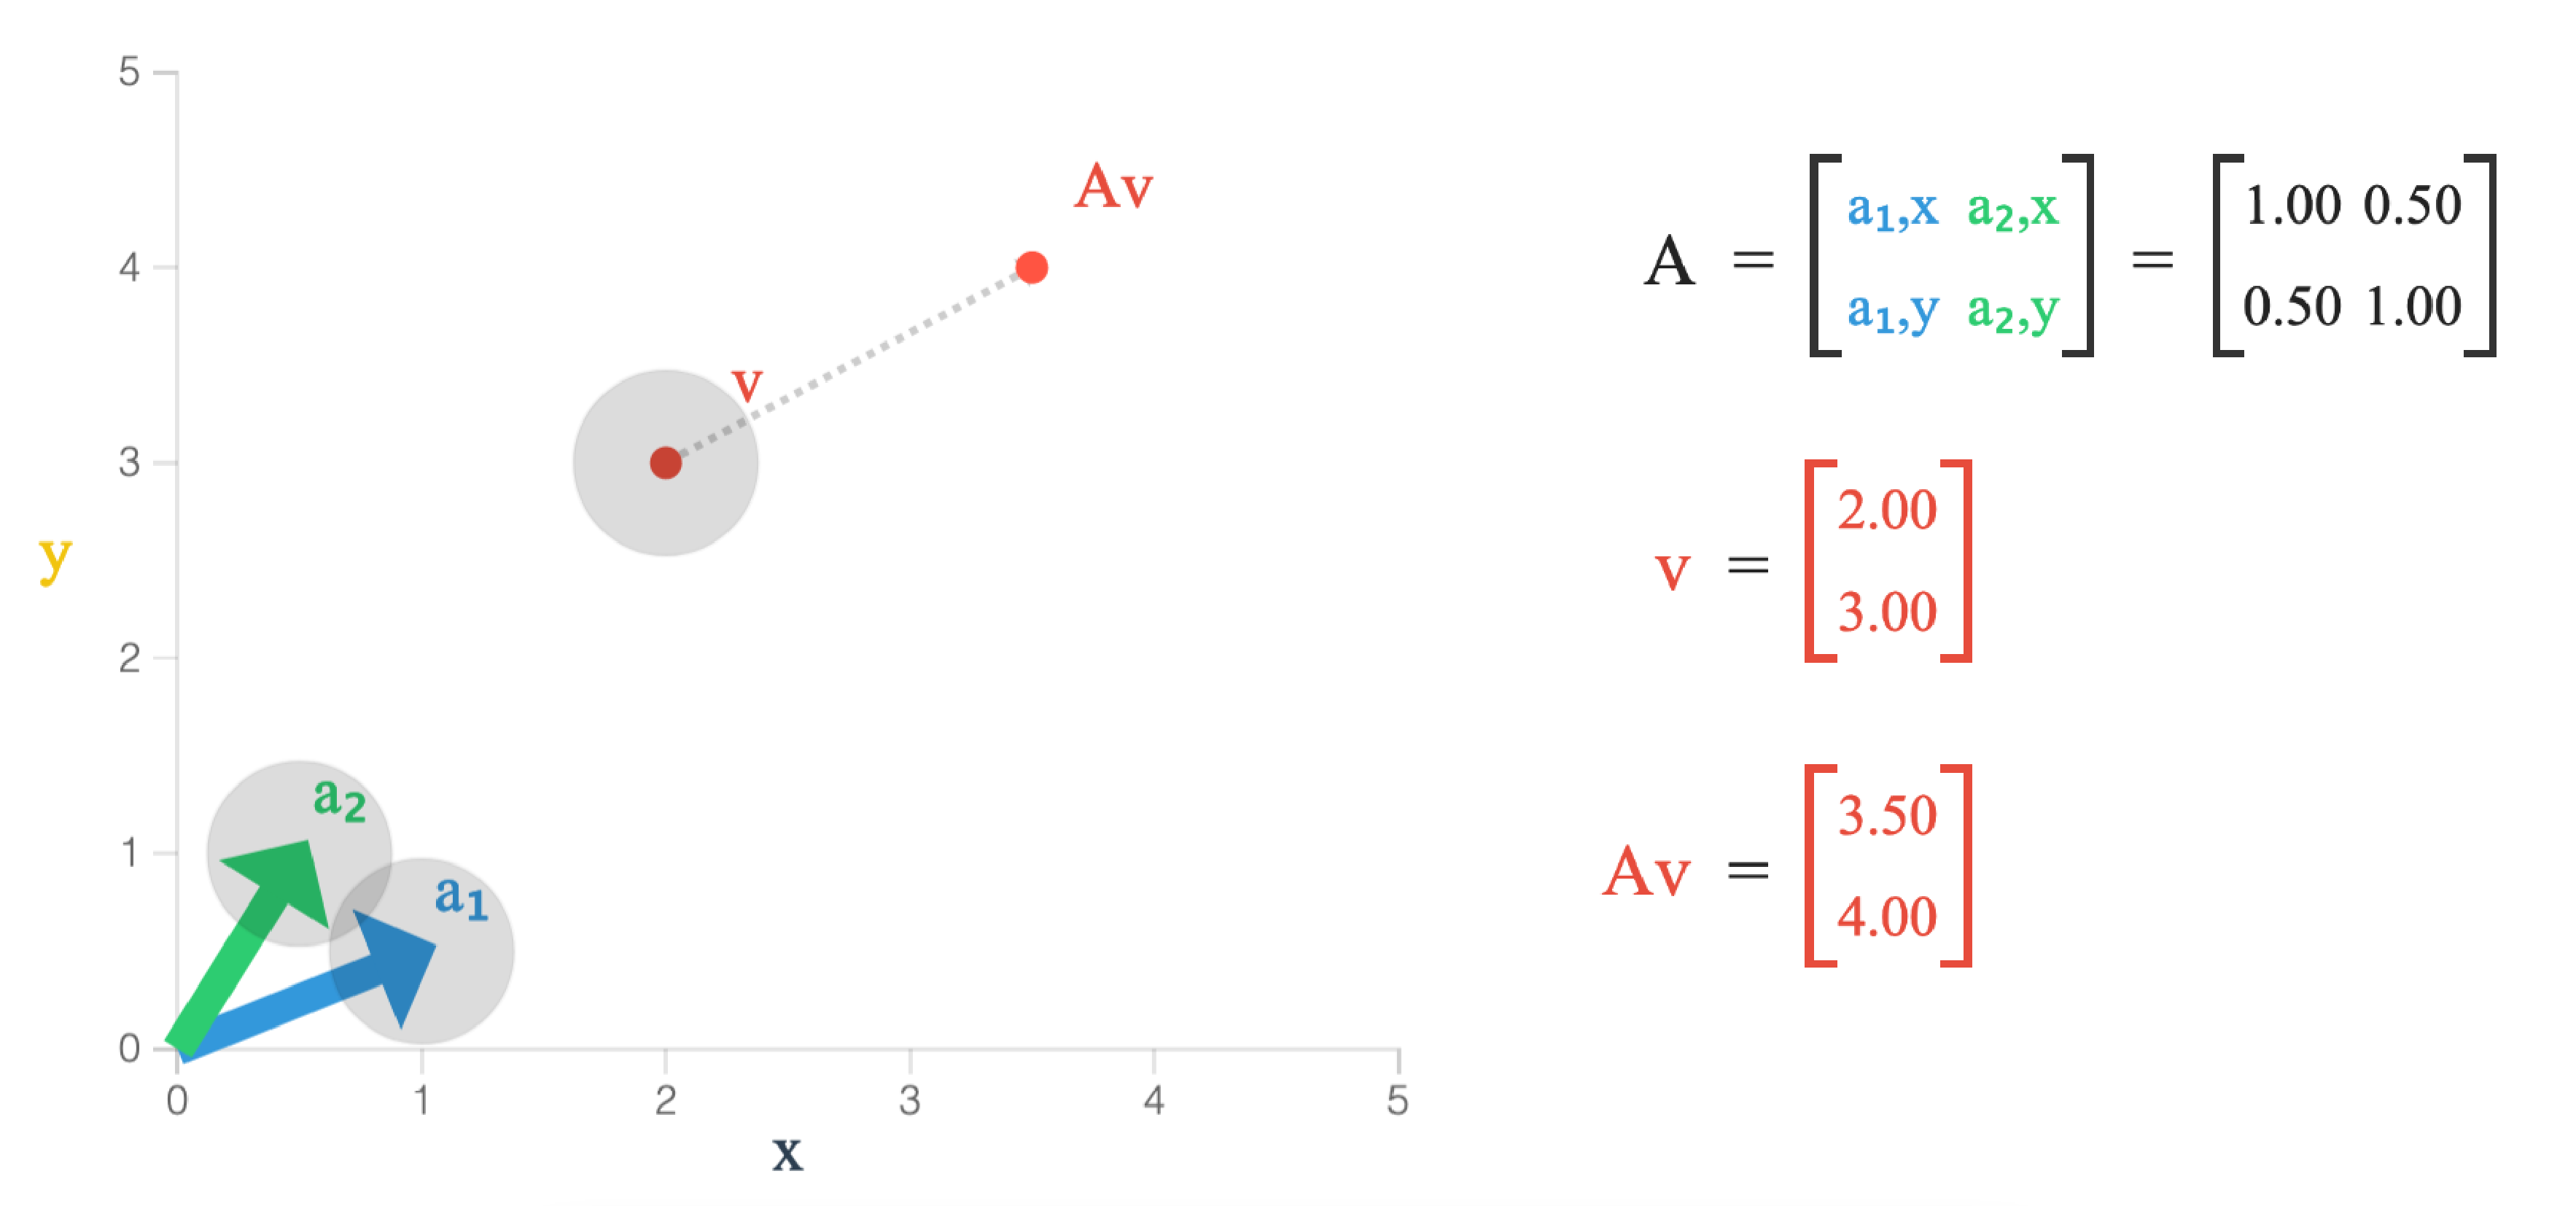
\includegraphics[width=0.8\linewidth]{assets/chapter-4/eigen-visually.pdf}
% \end{figure}

% Seeing what varies and what doesn't is an important form of \emph{feedback} that fosters conceptual understanding. The reader gains an initial understanding of how columns of $A$ impact $Av$’s value through interacting with the diagram: dragging any of $a_1$, $a_2$ and $v$ affects the position of $Av$. 

% In the original code repository~\footnote{\url{https://github.com/vicapow/explained-visually/tree/master/client/explanations/eigenvectors-and-eigenvalues}}, the authors wrote about a hundred lines of JavaScript with D3.js to make the first diagram. Although D3.js and Angular already provide significant support, it's still a lot of work to handle mouse down/up/hover events, and to keep track of intermediate values during dragging. 

% To reproduce this diagram in \Penrose, one can write a simple \Substance program in the linear algebra domain~\cite[Section 5.4]{penrose}. 

% \begin{figure}[h]
%     \centering
%     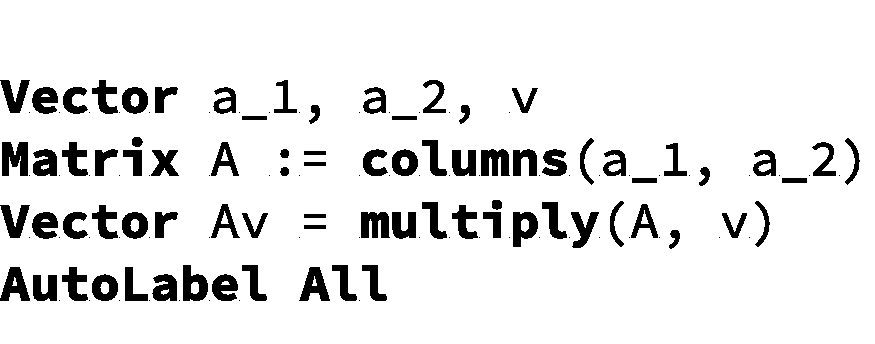
\includegraphics[width=0.4\linewidth]{assets/chapter-4/eigen-substance.pdf}
% \end{figure}

% With the core system, the trio generates a static SVG diagram. Under the hood, every \sub{Vector} is represented visually as an arrow starting at the origin ($a_1$, $a_2$), or a single point ($v$). They are all degrees of freedom (DOF) in the optimization problem. In other words, both the x and y-components of the arrow-end of  $a_1$, $a_2$, and the point representing $v$ are free to move on the canvas. Following the original design of the explorable, the system surfaces the DOFs as draggable points. Whenever the user drags the end of one of the arrows, the optimizer takes the new position as a part of the final solution, and solves the rest of the optimization problem. Effectively, by using this simple and generalizable strategy, which I will discuss in the following sections, the system can reproduce the interactive design using the \Penrose trio for a static diagram \emph{without a single line of code added}.

% \section{Semantics-preserving interactivity as feedback}
% \label{sec:semantic-drag}

% \begin{proposed}
% \cref{sec:ipenrose-example} is an example of a set of interactive behaviors that can be automatically derived from a \Penrose trio without any additional programming.  Specifically, the example leverages how \Penrose encodes visual semantics: \Penrose compiles a program trio to computational and optimization graphs with degrees-of-freedom (DOF)~\cite[Section 4.1.2-3]{penrose}. Degrees-of-freedom determine a diagram instance in \Penrose. They are ``free'' variables within the computational graph and non-constant root nodes in the optimization graph. DOFs are the key to generate a family of diagrams: by manipulating DOFs, the optimizer solves for different diagrams that satisfy the constraint set defined by the trio. In other words, DOFs are a concise representation for interaction. In this section, I use \emph{dragging} as a case study and show a few ways of manipulating the DOFs in a semantics-preserving manner. 

% As a reasonable default, the system can find positional properties in the DOFs and make them draggable. In \cref{sec:ipenrose-example}, the relevant \Style blocks define a simple computational graph for the \Substance program, where \sty{a_1.data}, \sty{a_2 .data}, and \sty{v.data} are DOFs. \cref{fig:eigen-comp-graph} shows the graph for \sty{a_1}’s properties. To accomplish the interactivity in the example, the system can analyze the computational graph to find DOFs and their aliases, \ie, child nodes that are assigned values of the DOFs. For instance, \sty{a_1.data} is a DOF and \sty{a_1.icon.end} references \sty{a_1.data}. In contrast, \sty{Av.end} is not made draggable because it's not a DOF nor an alias in the computational graph: its value is computed by \sty{matmul(a_1.data, a_2.data)}.

% \vspace{10pt}
% \begin{figure}[h]
%     \centering
%     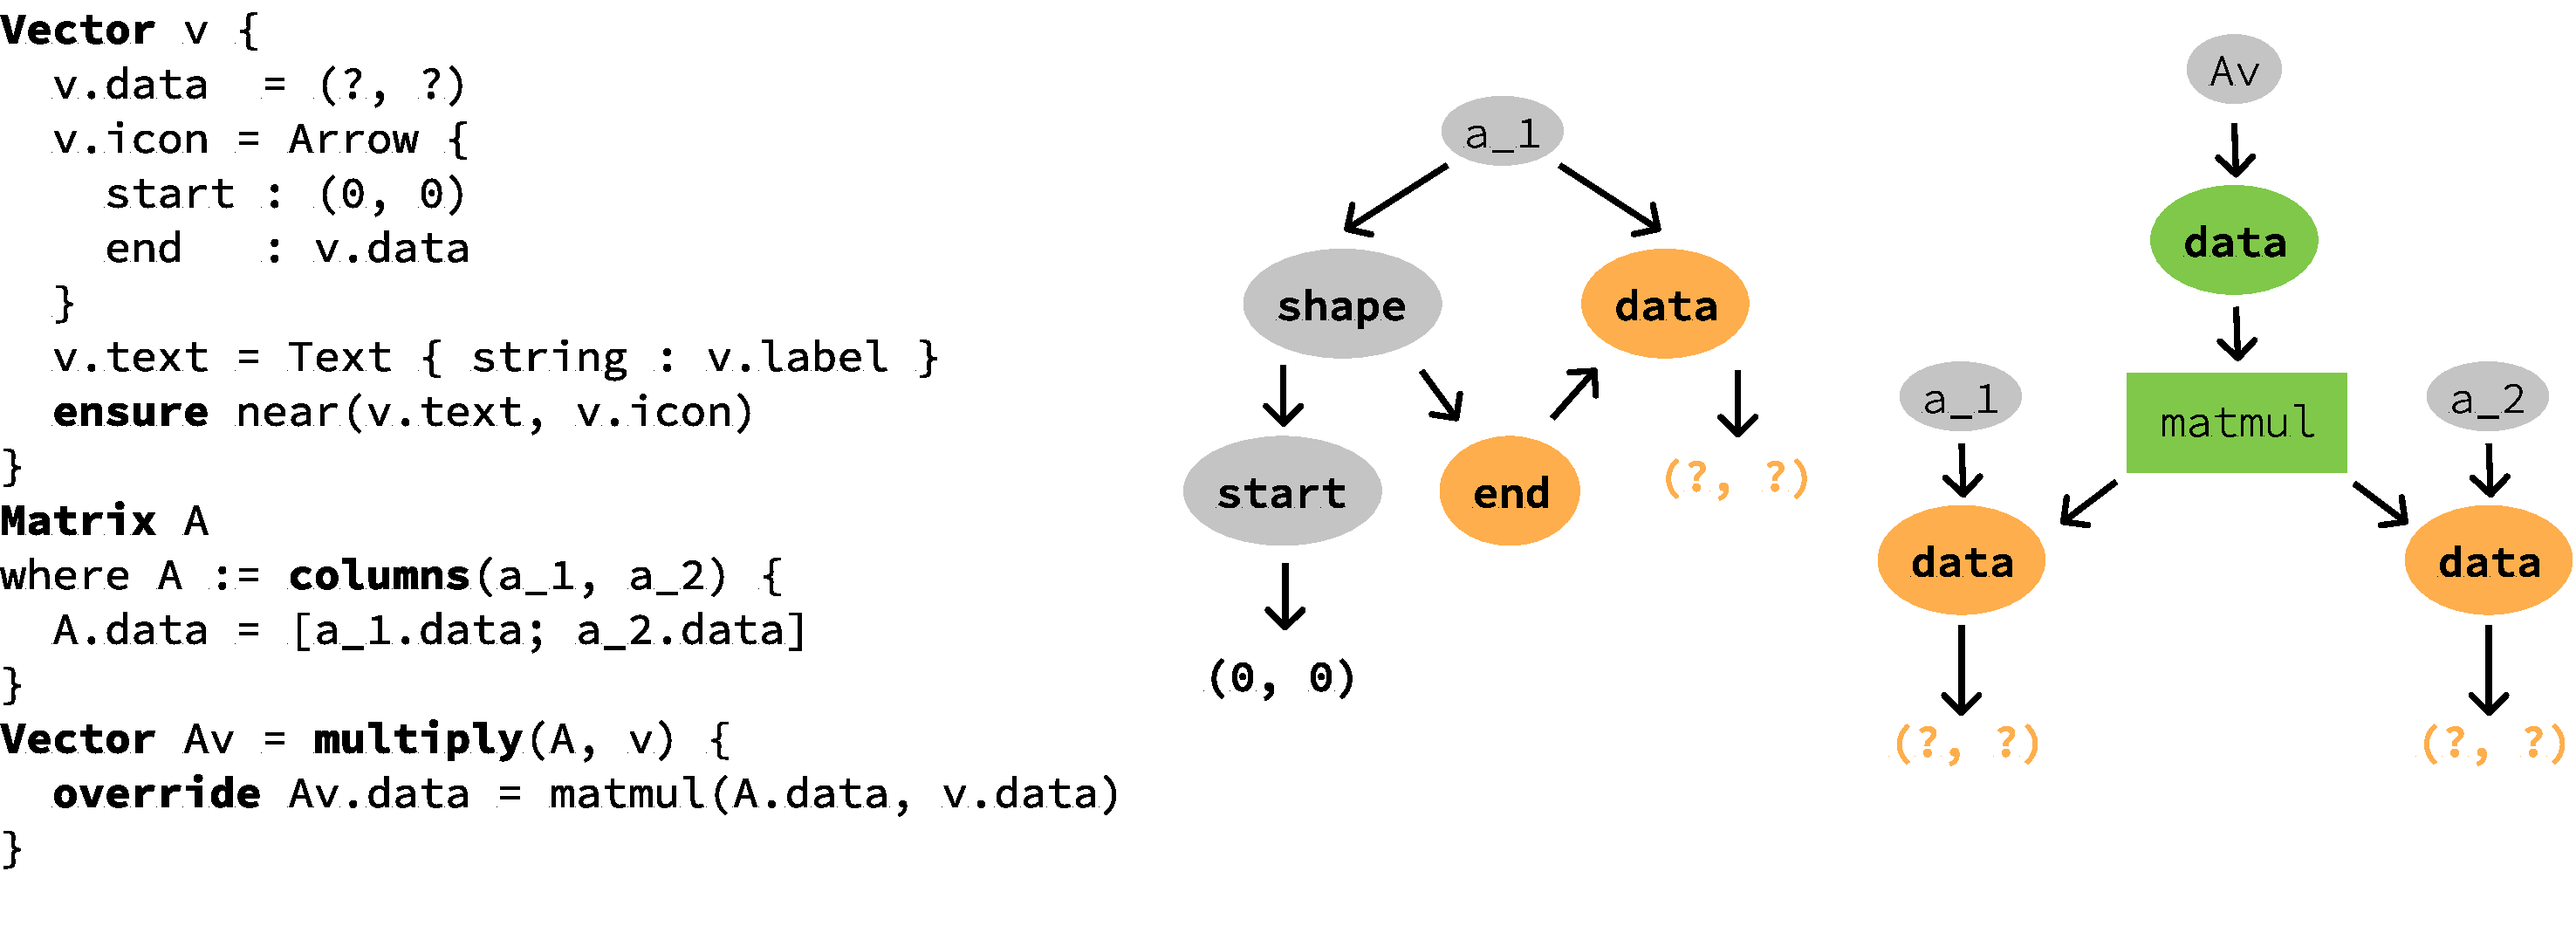
\includegraphics[width=\linewidth]{assets/chapter-4/eigen-comp-graph.pdf}
%     \vspace{-30pt}
%     \caption{\textbf{Left}: relevant blocks in the linear algebra \Style program for \cref{sec:ipenrose-example}. \textbf{Right}: computational graphs for \texttt{a\_1} and \texttt{Av}, where the \texttt{data} field for the former is optimized and that for the latter is computed.}
%     \label{fig:eigen-comp-graph}
% \end{figure}
% \vspace{10pt}

% Once exposed as draggable properties, the user can now change the values of positional DOFs by dragging shapes around. However, since their interaction is situated in an optimization problem, it's important to discuss how an optimizer influences this interaction and manipulates the rest of the diagram in a semantics-preserving way. In \cref{sec:ipenrose-example}, dragging \sty{a_1.icon.end} and \sty{a_2.icon.end} works as intended because they are independent from each other: they don't participate in the same constraints in the computational graph. However, this is not the right interaction for DOFs that participate in the same constraints, which is often the case. In this section, I give two example optimization strategies for supporting semantics-preserving drag.    
% \subsection{Follow the cursor}
% \label{sec:follow-the-cursor}

% \vspace{10pt}
% \begin{figure}[h]
%     \centering
%     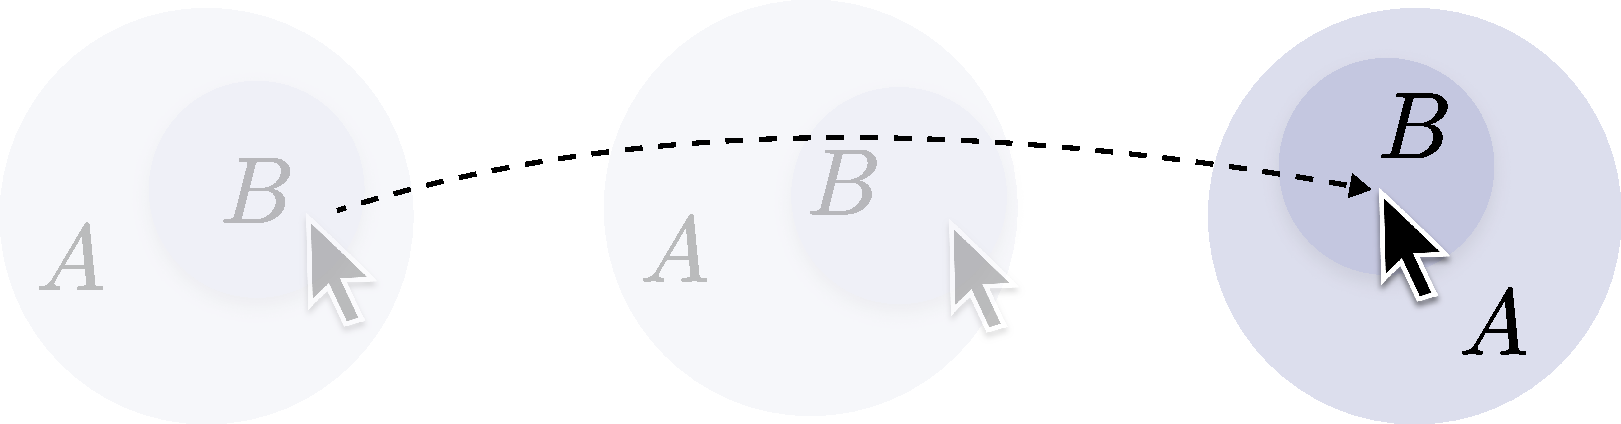
\includegraphics[width=0.8\linewidth]{assets/chapter-4/drag-expected.pdf}
%     \caption{Dragging a subset, $B$, in a Venn diagram in an intuitive and semantics-preserving way, where $B$ is always under the cursor and $B \subset A$ is always held true.}
%     \label{fig:drag-expected}
% \end{figure}
% \vspace{10pt}

% Consider the example in \cref{fig:drag-expected}, which shows a simple Venn diagram of sets $A$ and $B$ where $B \subset A$. The underlying rule of this visual representation is that a subset is always visually contained in the superset. An interactive diagram should clearly reveal this rule by keeping this containment relationship true at all times. For instance, if a student drags $B$ to the right, the diagram should change such that $A$ still contains $B$. Importantly, the interaction should be natural, and also make the feedback very clear: as the student is dragging $B$, $B$ must stay under the cursor, and the rest of the diagram should incrementally move with $B$ to maintain the containment relationship.

% Unfortunately, when using the current \Penrose optimizer, dragging either $A$ or $B$  yields counterintuitive results: the optimizer changes arbitrary properties, including the manipulated ones. This is because it optimizes all DOFs simultaneously. In \cref{fig:drag-default}, it moves both $A$ and $B$ to satisfy the containment constraint.  This behavior adds noise to the feedback, and may confuse the student.

% \vspace{10pt}
% \begin{figure}[h]
%     \centering
%     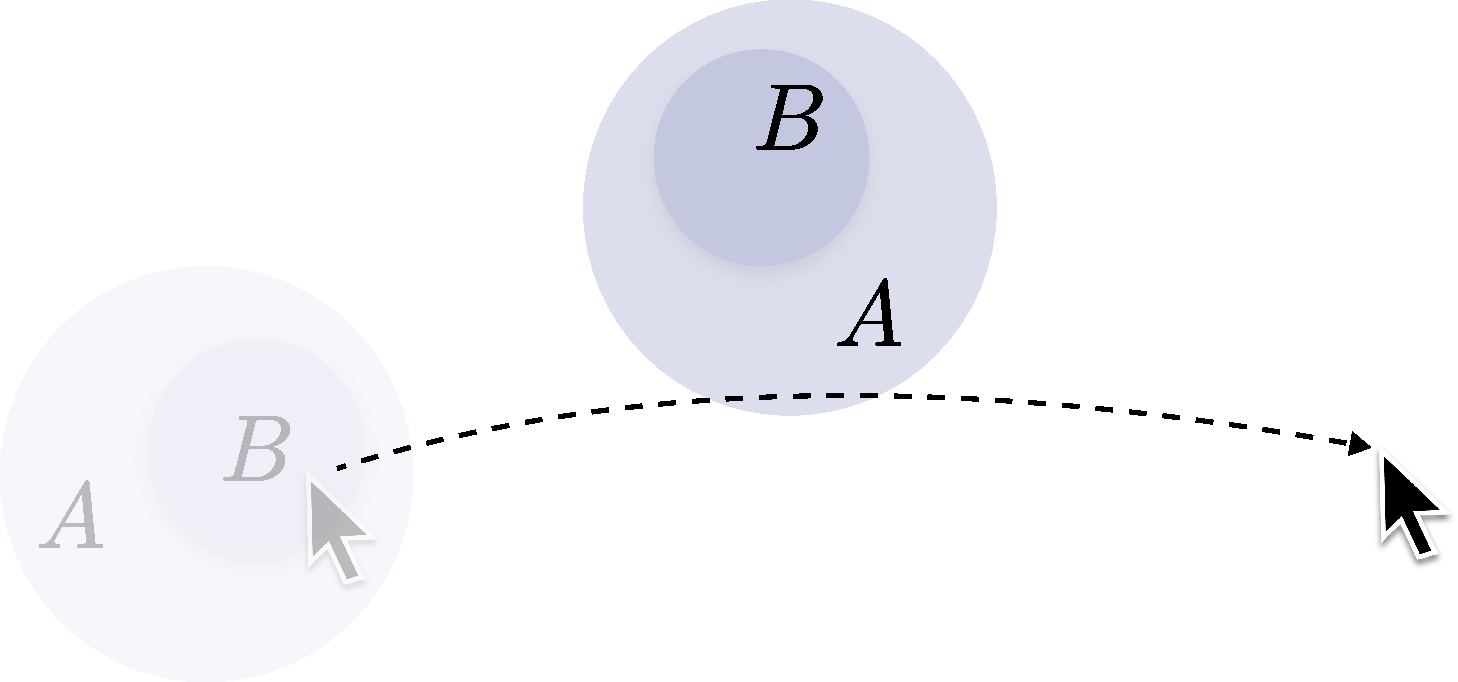
\includegraphics[width=0.75\linewidth]{assets/chapter-4/drag-default.pdf}
%     \caption{Dragging a subset, $B$, in a Venn diagram in semantics-preserving but counterintuitive way, where $B \subset A$ held true but the shapes appear in random locations.}
%     \label{fig:drag-default}
% \end{figure}
% \vspace{10pt}

% To enable intuitive interactivity, the system can analyze the computational graph again to derive the right behavior. We can achieve this behavior by ``locking'' the DOFs, treating them as constants in the optimizer. Specifically, when a student manipulates DOFs or its aliases, the system locks these DOFs and optimizes the rest as usual. When the student interacts with an object (\ie, dragging to change \sty{x} and \sty{y} of a \sty{Circle}), the system yields the control to the student completely and locks the manipulated properties during optimization. The visual effect is that all other parts of the diagram ``follow'' the student interaction. 

% \subsection{Freeze the world}
% \label{sec:freeze-the-world}

% Locking the manipulated property is not the only way to maintain the visual semantics. Instead of limiting the optimizer, we could also limit the interaction so they see the effect of changing one or multiple shape properties under constraints. When the student interacts with a shape, the optimizer keeps all other properties locked and continuously uses the energy function to “guide” the student. The techniques involved are different from \cref{sec:follow-the-cursor}. In this case, the student is playing the role of the optimizer, \ie, changing DOFs, while the optimizer only sends feedback to make sure the interaction is semantic. The visual effect is a constrained interaction where the student can only make semantically-valid moves. 

% \vspace{10pt}
% \begin{figure}[h]
%     \centering
%     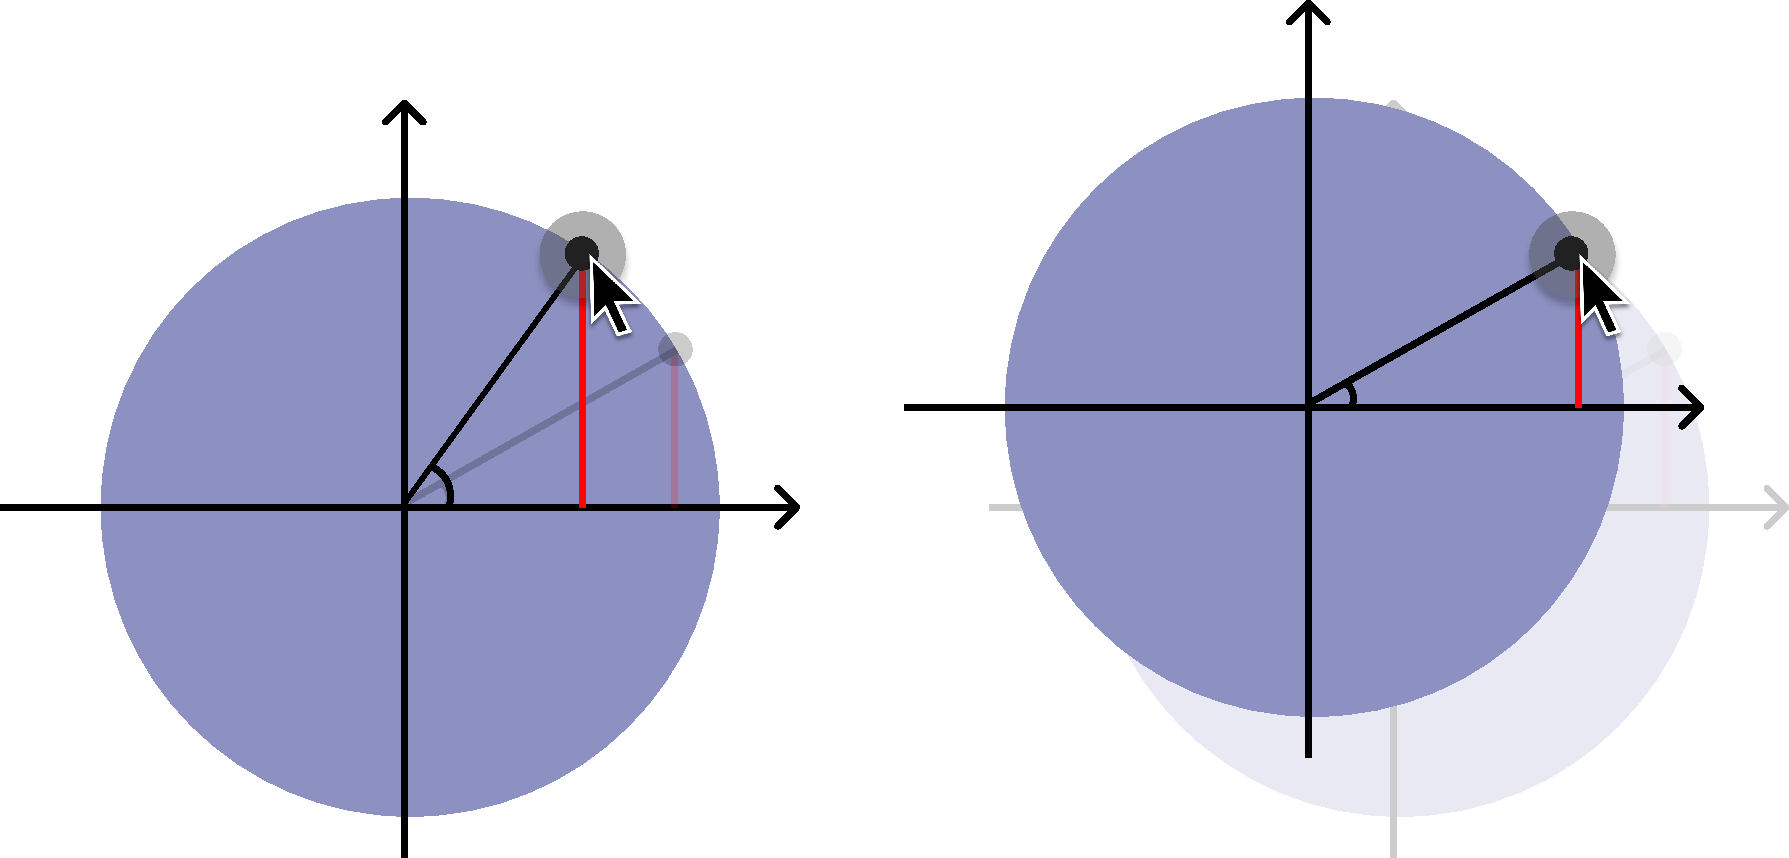
\includegraphics[width=0.75\linewidth]{assets/chapter-4/unit-circle-drag.pdf}
%     \caption{The behavior of dragging a point along the unit circle depends on the optimization strategy. \textbf{Left}: ``Follow the cursor'' shifts the entire diagram to follow the point and doesn't correspond to the mathematical semantics. \textbf{Right}: ``Freeze the world'' should be the correct optimization strategy, where the point only moves along the circle, and nothing else changes in the diagram.}
%     \label{fig:unit-circle-drag}
% \end{figure}
% \vspace{10pt}


% For instance, \cref{fig:unit-circle-drag} shows a diagram of the unit circle. A natural interaction is to drag the point along the unit circle to see how the values of trig functions change. In this case, the red line shows the value of $sin$. If the optimizer naively follows the cursor, \cref{fig:unit-circle-drag} (right) would be the result, where the rest of the diagram is translated to stay in a valid layout. Instead, it's much more desirable to ``freeze the world'' and constrain the student input within the feasible region—--along the unit circle (\cref{fig:unit-circle-drag} left).

% Together, these two strategies cover a wide range of drag behaviors that are traditionally difficult and time-consuming to implement. Note that these two strategies are not necessarily mutually exclusive. In fact, the system may have a set of default rules for or let the author specify the strategy on a per-DOF basis. For instance, an instructor might apply ``freeze the world'' to show students the valid positions of a component in a diagram, while applying ``follow the cursor'' to the rest of the components to show alternative layouts of the diagram. 


% \vspace{10pt}
% \noindent\textbf{Encoding optimization strategies.} If the author wants to control the optimization strategy, they will need an encoding to do so. Because \Style already has language constructs for matching on shapes, a \Style language extension may be suitable for specifying static strategies per shape, \eg, a shape should always follow the cursor when dragged. However, the current design of \Style may not be suitable for deciding strategies dynamically if needed, \eg, a shape follows the cursor in a certain region of the diagram, and freezes the world on the boundary. 
% \end{proposed}

% \section{Highlighting and annotation as feedback}
% \label{sec:highlight-and-annotate}

% \begin{proposed}

% As demonstrated in \cref{chp:edgeworth}, diagram understanding is a vital step towards representational fluency. A significant part of diagram understanding maps to learning the translational semantics of a diagram, \ie, which shape represents what math object. While \Edgeworth helps students practice the mapping between a particular visual representation and symbols, I propose to \textbf{provide on-demand, inter-representational feedback by utilizing the translational semantics of a \Penrose trio}. 

% \subsection{Inter-representational highlighting}

% Students' exposure to visual representations is often limited by traditional media like textbooks and in-person lectures. The mapping between symbolic and visual representations is often scarcely presented via prose, gesture, and carefully designed worked examples. Web-based materials show a much more pervasive use of on-demand highlighting to build up inter-representational connections. However, there’s also a non-trivial authoring burden to meticulously annotate the HTML document and the diagram with CSS classes:

% \vspace{10pt}
% \begin{figure}[h]
%     \centering
%     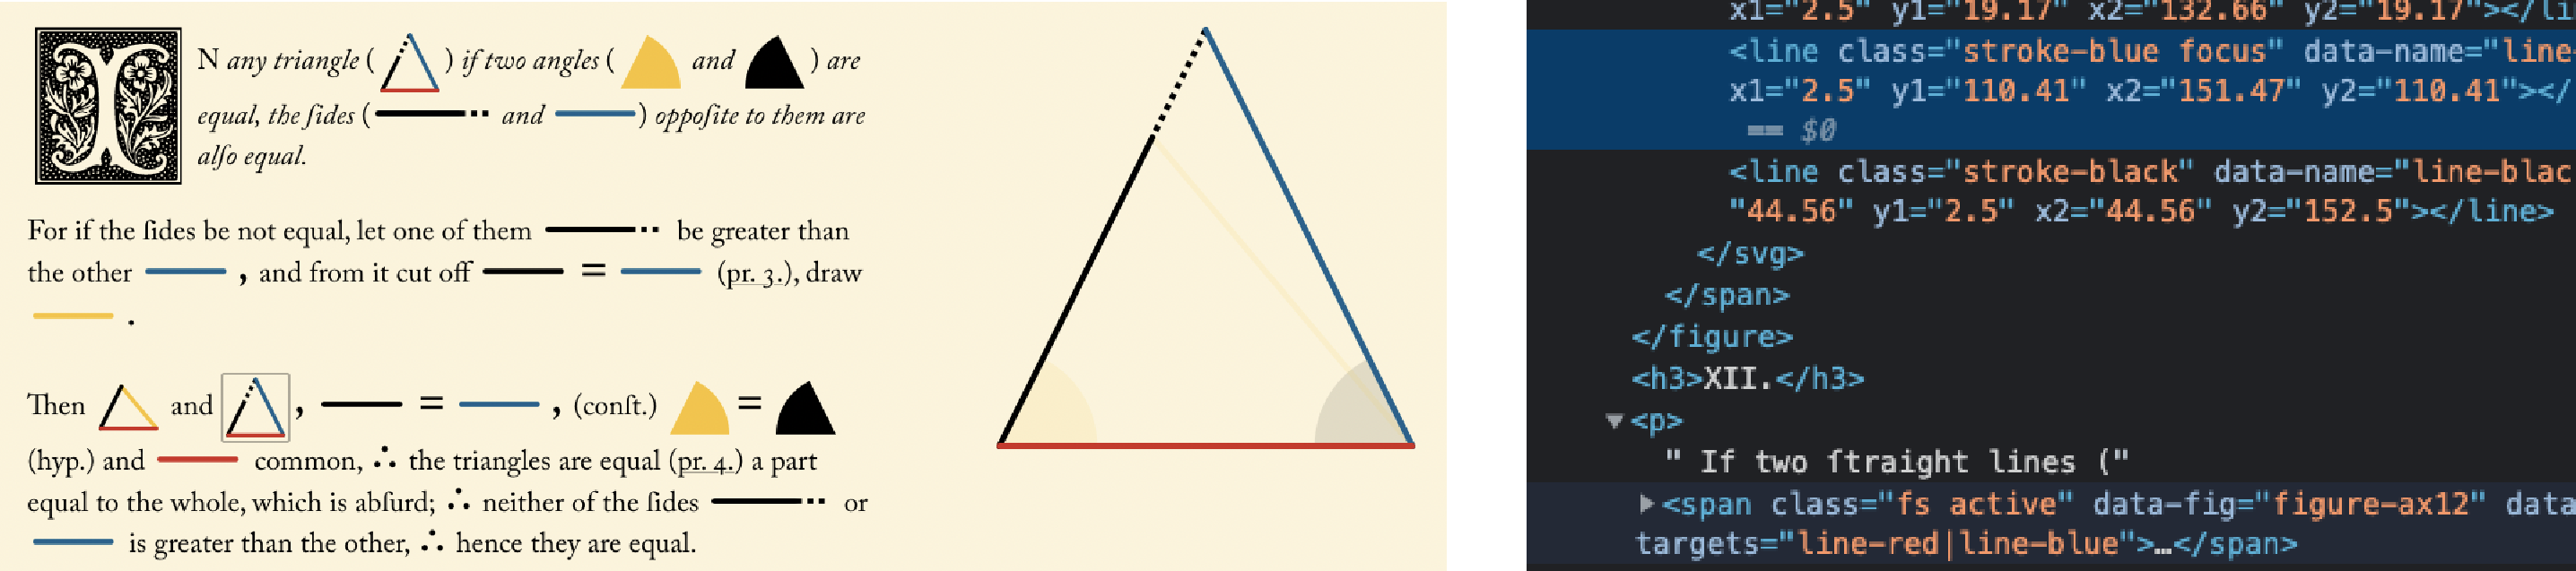
\includegraphics[width=\linewidth]{assets/chapter-4/euclid-highlight.pdf}
%     % \label{fig:euclid-highlight}
% \end{figure}
% \vspace{10pt}

% If an online textbook or website uses diagrams generated by \Penrose, the author may leverage the translational semantics to automatically provide on-demand highlights. For instance, suppose an author writes an visual explanation in markdown with interleaving \Substance symbols in the prose. The system can automatically generate diagrams by extracting the \Substance symbols and provide highlights for all subsequent references to the same symbols. Since \Penrose can generate alternative diagrams in the same visual presentations, the highlighting can also provide contrasting cases of a particular entity across diagram instances.

% \vspace{10pt}
% \begin{figure}[h]
%     \centering
%     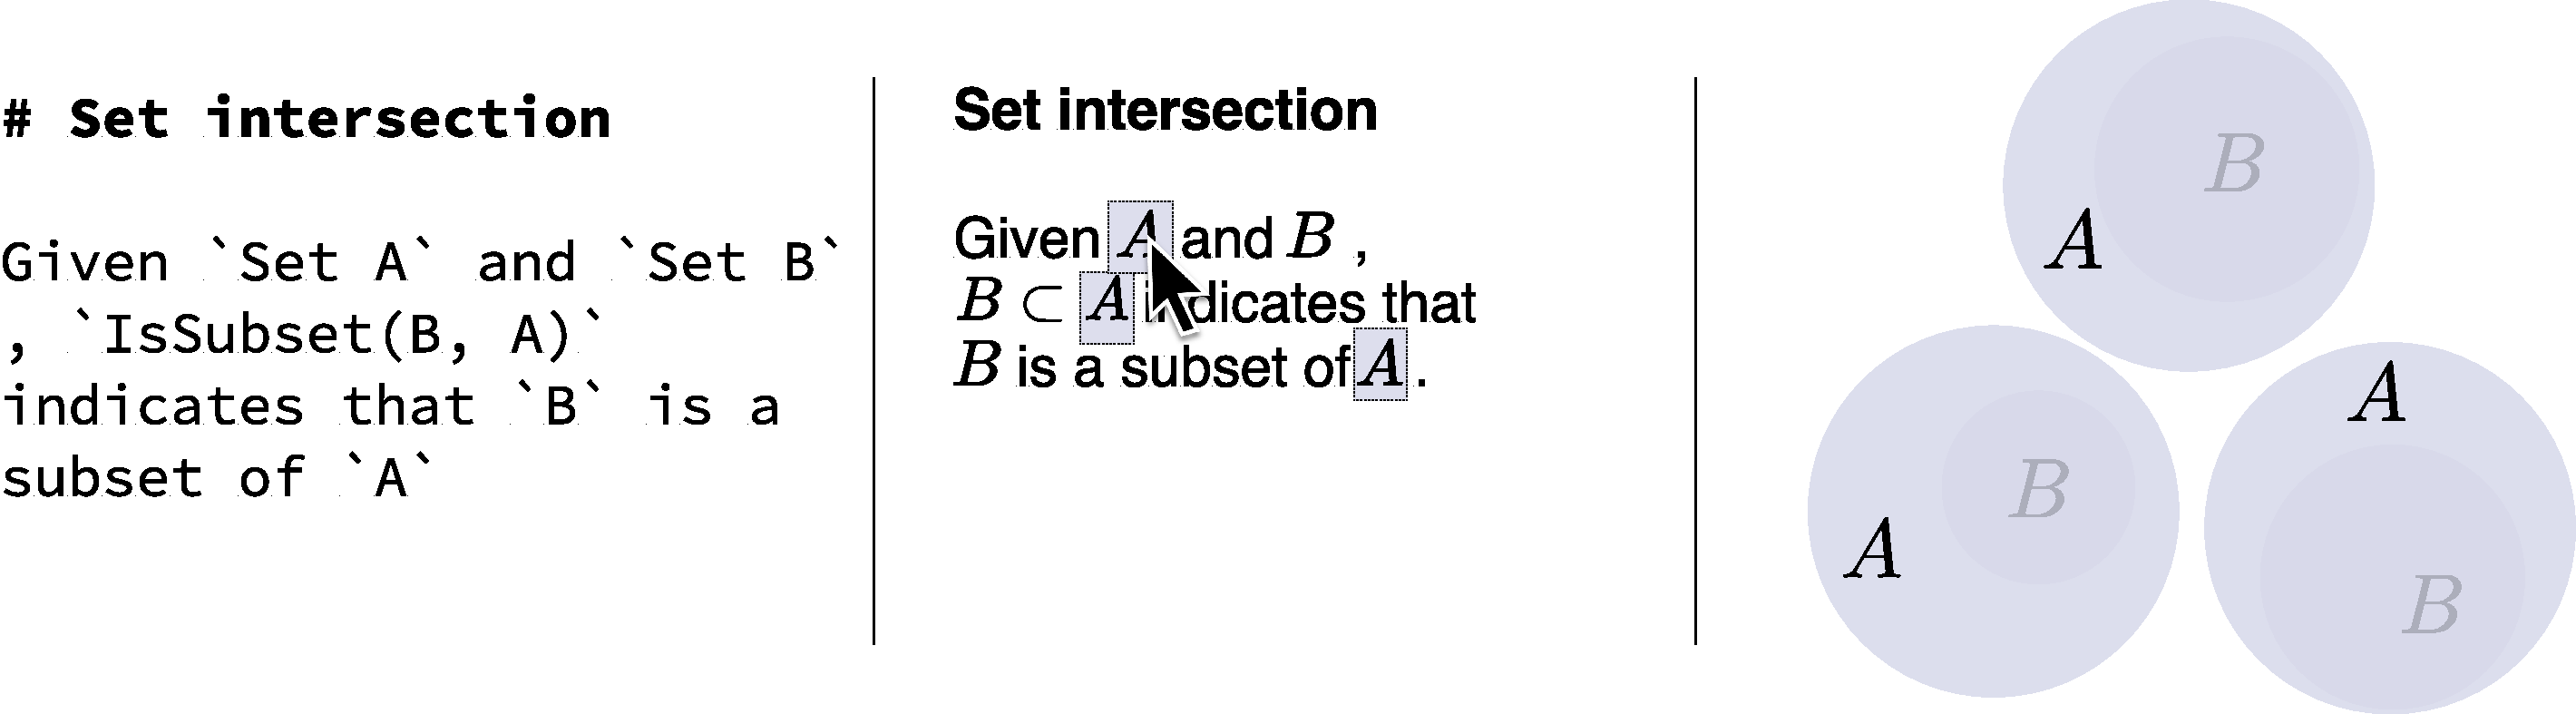
\includegraphics[width=\linewidth]{assets/chapter-4/markup-highlight.pdf}
% \end{figure}
% \vspace{10pt}

% Building connections among multiple visual representations also improve learning~\cite{multipleReps}. Because a \Penrose trio is representationally salient, one can swap among alternative \Style programs to get diagrams that visualize the same symbols. Because the \Substance program stays the same, the same strategy also works for highlighting diagram parts across multiple visual representations.

% \vspace{10pt}
% \begin{figure}[h]
%     \centering
%     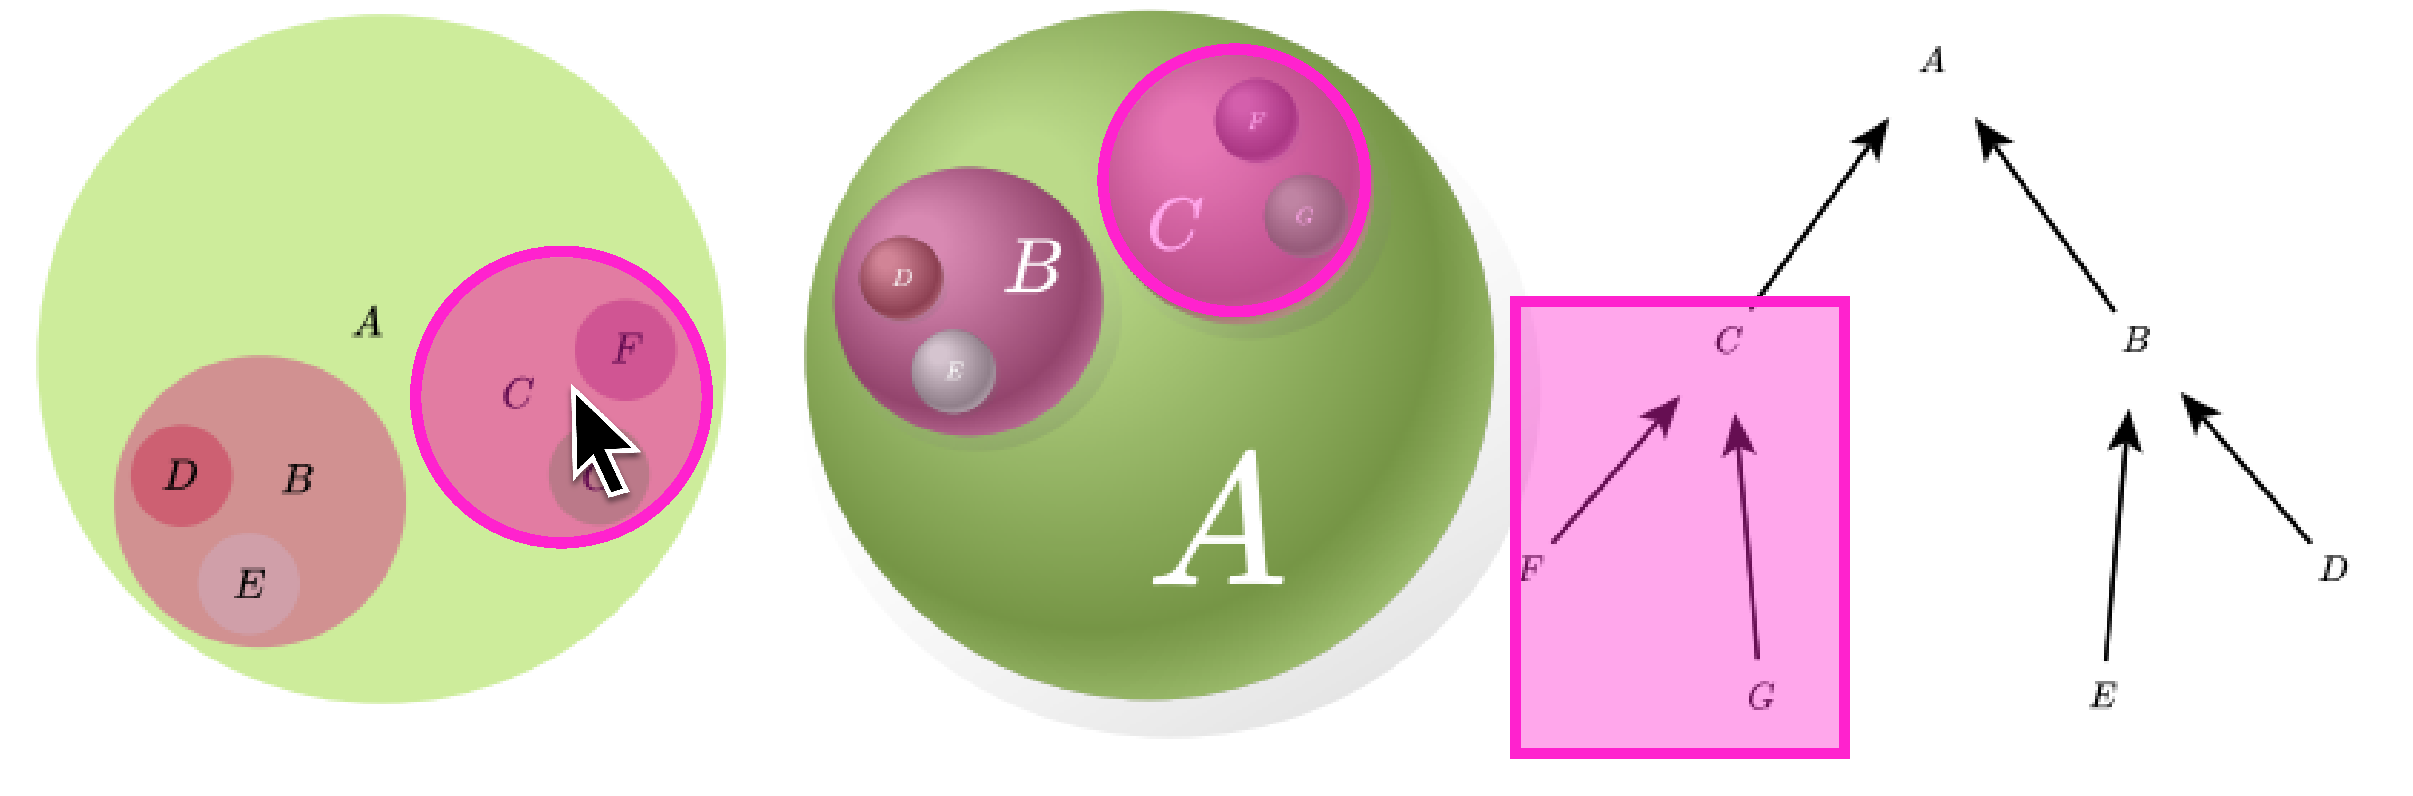
\includegraphics[width=0.9\linewidth]{assets/chapter-4/multirep-highlight.pdf}
% \end{figure}
% \vspace{10pt}

% \subsection{Documentation and program slices as tooltips} 

% \vspace{10pt}
% \begin{figure}[h]
%     \centering
%     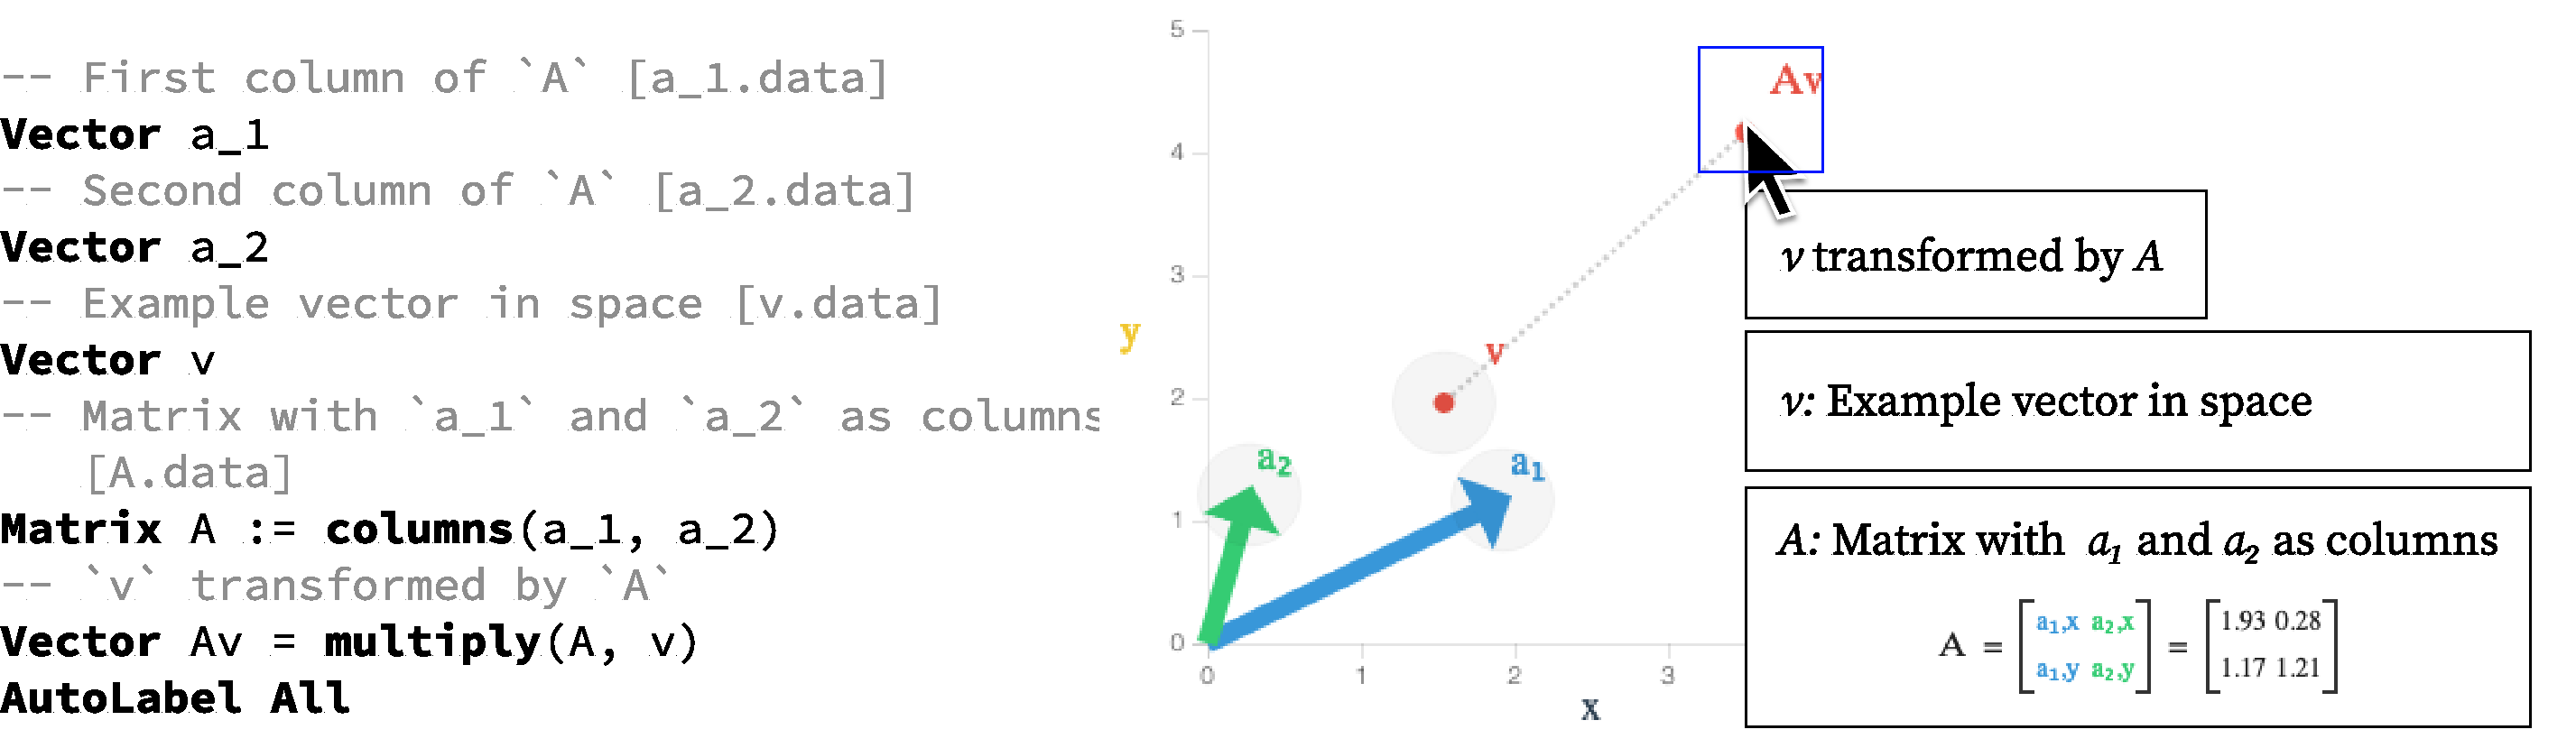
\includegraphics[width=\linewidth]{assets/chapter-4/docs-tooltips.pdf}
% \end{figure}
% \vspace{10pt}

% In technical documents, symbols and acronyms are often defined once and used everywhere else. To help readers understand them, tools like ScholarPhi and Nota~\cite{scholarPhi, nota} use tooltips to aid readers. In real world publications, authors augment math equations for better readability, too. Diagrams use even more symbolism and can be hard to understand. We propose a lightweight markup language in the form of \Substance documentation for authoring simple \emph{diagram augmentation}. Similar to Idyll~\cite{idyll}, the markup language has a markdown-like syntax, but allows splices of \Substance variables and runtime values. In the frontend, we analyze the \Substance values in each snippet, and trace all related snippets based on variable references. For instance, the snippet about $Av$ refers to both $A$ and $v$, so they appear on the tooltip stack.

% The translational semantics also involve how \Domain, \Substance, and \Style programs relate to each other. Therefore, \Style and \Domain can also be valuable sources of feedback: the \Style program encodes the visual semantics, and the \Domain program captures the grammar of notations. A slice of a \Penrose trio traces the origin of a graphical primitive to the \Domain, \Substance, \Style programs. For instance, without any authoring burden, the system can display slices of the program trio based on object selection. Alternatively, the proposed markup language may be extended to \Domain and \Style, and the system can render inline documentations in all three languages.

% \vspace{10pt}
% \begin{figure}[h]
%     \centering
%     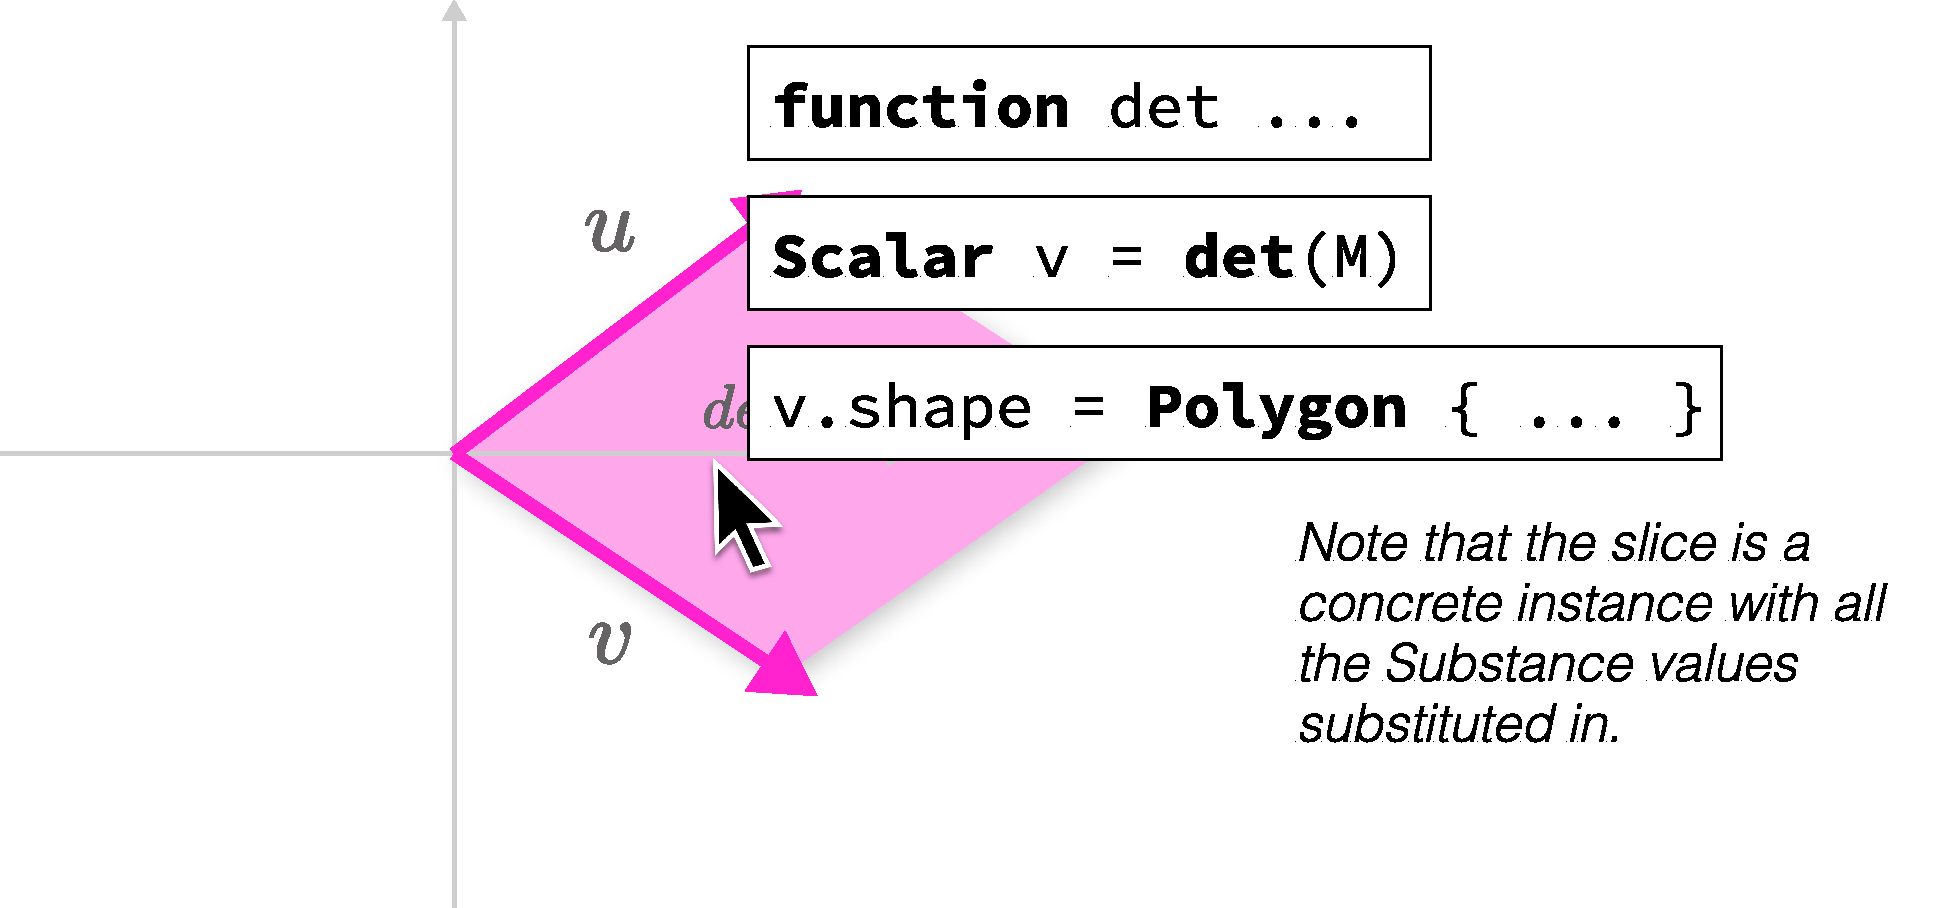
\includegraphics[width=0.75\linewidth]{assets/chapter-4/slices.pdf}
% \end{figure}
% \vspace{10pt}
% \end{proposed}

% \section{Evaluation}

% \begin{proposed}
% To evaluate the discussed interactive techniques, I plan to conduct comparative case studies between feature-full modern JavaScript libraries (e.g. D3.js) and \Penrose. Research questions for this study include:
% \begin{itemize}
%     \item Does the \Penrose-based system simply programming interactive diagrams?
%     \item Are the interactive features comparable to the hand-written examples? 
%     \item How expressive is our grammar of interactivity?
%     \item When does the approach break down?
% \end{itemize}

% In general, I expect that our system can cover common, important interactive features with significantly less manual effort. In the studies, I plan to collect both quantitative (\eg, lines-of-code, time taken) and qualitative data about authoring interactive diagrams using JS library versus our system. Currently, the candidate pool of examples include:

% \begin{itemize}
% \item Worked examples and explorable explanations:
%     \begin{itemize}
%         \item A Gentle Introduction to Graph Neural Networks: \url{https://distill.pub/2021/gnn-intro/}
%         \item Explained visually: \url{https://setosa.io/ev/}
%         \item Explorable explanations: \url{https://explorabl.es/}
%         \item Gallery of concept visualization: \url{https://conceptviz.github.io/}
%     \end{itemize}
% \item Online textbooks and curricula:
%     \begin{itemize}
%         \item Seeing theory: \url{https://seeing-theory.brown.edu/}
%         \item Immersive math: \url{http://immersivemath.com/ila/index.html}
%         \item Mathigon: \url{https://mathigon.org/}
%         \item Physically-based rendering: \url{https://pbr-book.org/}
%         \item Brilliant: \url{https://brilliant.org/}
%     \end{itemize}
% \end{itemize}
% \end{proposed}

\section{Concluding remarks}

Curiously, building authoring tools for rich, interactive diagrams, narratives, and learning activities seems just the right amount of material for a second dissertation,\footnote{In the spirit of \citet{barik_error_nodate}} or a full-time job.

% \appendix
% % HACK: disable page numbering
\pagenumbering{gobble}

\chapter{\Edgeworth project plan}

To address the committee feedback from the thesis proposal presentation, this appendix to the proposal document elaborates on \cref{chp:edgeworth}. This elaboration comes in acknowledgment that the committee sees the goals in \cref{chp:ipenrose} as optional.  In this appendix, I summarize the proposed elaboration on \cref{chp:edgeworth}, describe the research hypotheses, and outline the evaluation plan for validating them. The intention of this appendix is to specify all of the required work in the dissertation.

% In the proposal document, \cref{chp:edgeworth} describes the following completed work on \Edgeworth:

% \begin{itemize}
%     \item Formative interviews with 6 educational content authors
%     \item Design and implementation of mutation operators in the \Edgeworth mutator
%     \item A prototype of the \Edgeworth mutator with a configuration-based workflow
%     \item Preliminary evaluation of the prototype by re-creating problems in a geometry textbook
% \end{itemize}


\section{Definitions}
\label{sec:definitions}

In the discussion of translation problems, \cref{chp:edgeworth} uses terms such as ``instance,'' ``noninstance,'' ``near hit,'' and ``near miss.'' To standardize the terminologies in this appendix, I give some definitions here.

Given a set of mathematical statements describing logical entities and their relationships, a diagram can be associated with them in one of the following ways:

\vspace{0.5em}
\begin{figure}[h]
\begin{minipage}[b]{0.48\linewidth}
$\bullet$ \textbf{Example}: the diagram represents the math statements, \ie all the statements hold true in the diagram. 
    \vspace{3pt}
    
$\bullet$ \textbf{Counterexample}: the diagram clearly violates the math statements, \ie one or more statements are false in the diagram.
    \vspace{3pt}
    
$\bullet$ \textbf{Positive edge case}: the diagram is an example of the math statements, but contains extraneous entities and/or more specialized relationships. 
    \vspace{3pt}
    
$\bullet$ \textbf{Negative edge case}: the diagram is a counterexample, but only requires a few changes to become an example.
\end{minipage}
\hfill
\begin{minipage}[b]{0.45\linewidth}
    \centering
    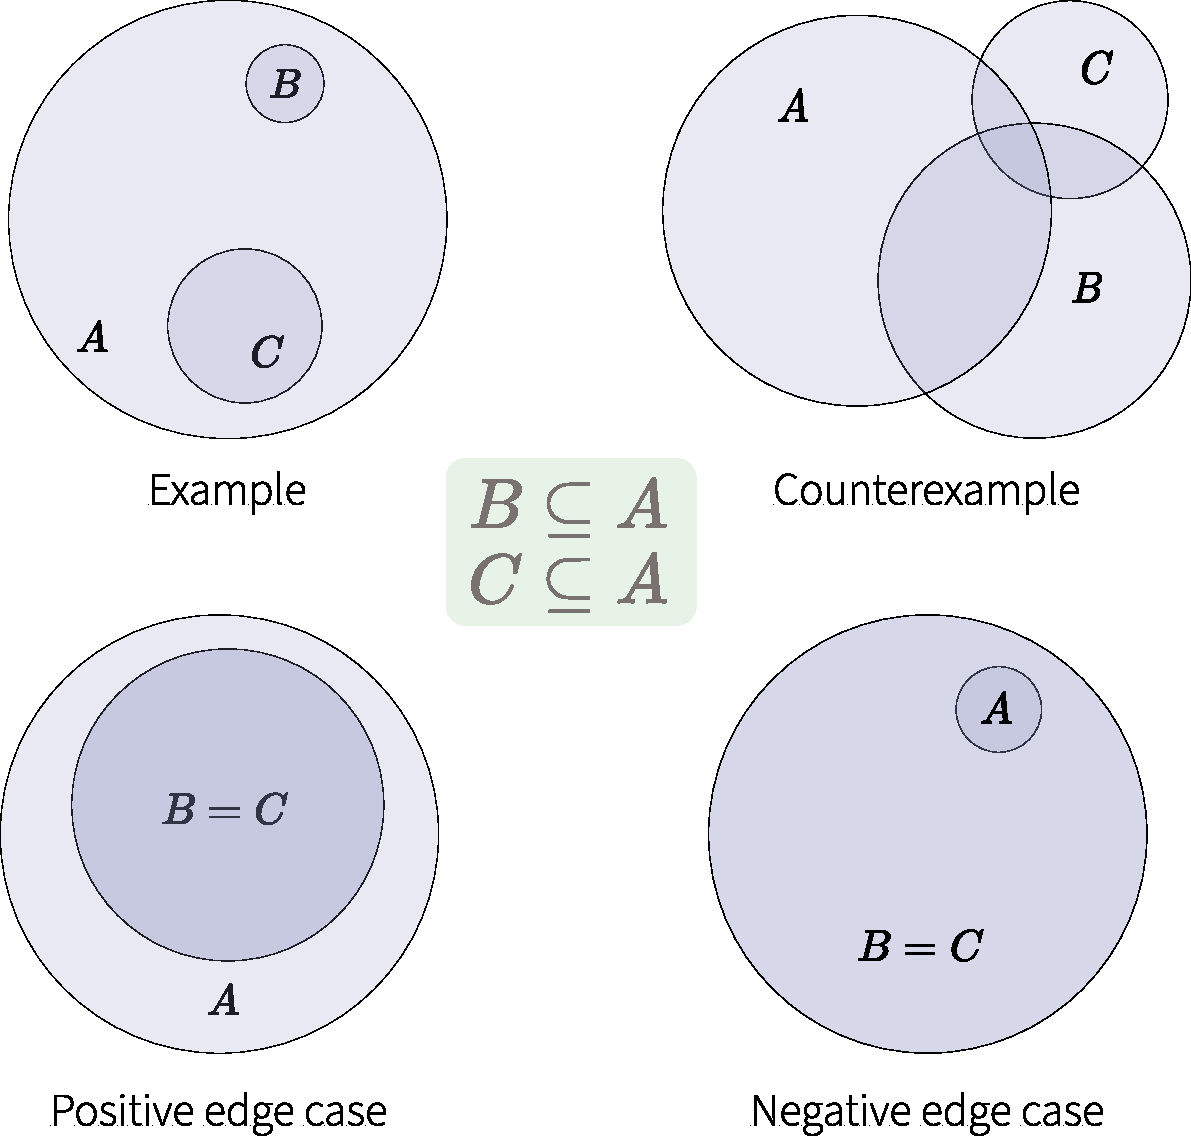
\includegraphics[width=\textwidth]{assets/appendix/definitions-examples.pdf}
\end{minipage}
\end{figure}

% While distinguishing between examples and counterexamples is often straightforward, identifying edge cases can depend on the context. For instance, the counterexamples in the figure above both violate all math statements, but the lower-right diagram can be considered an edge case because one can swap the labels $A$ and $B$ to make it an example. 

\section{Summary of proposed work}

\subsection{Programming-by-example workflow}


\begin{figure}
    \centering
    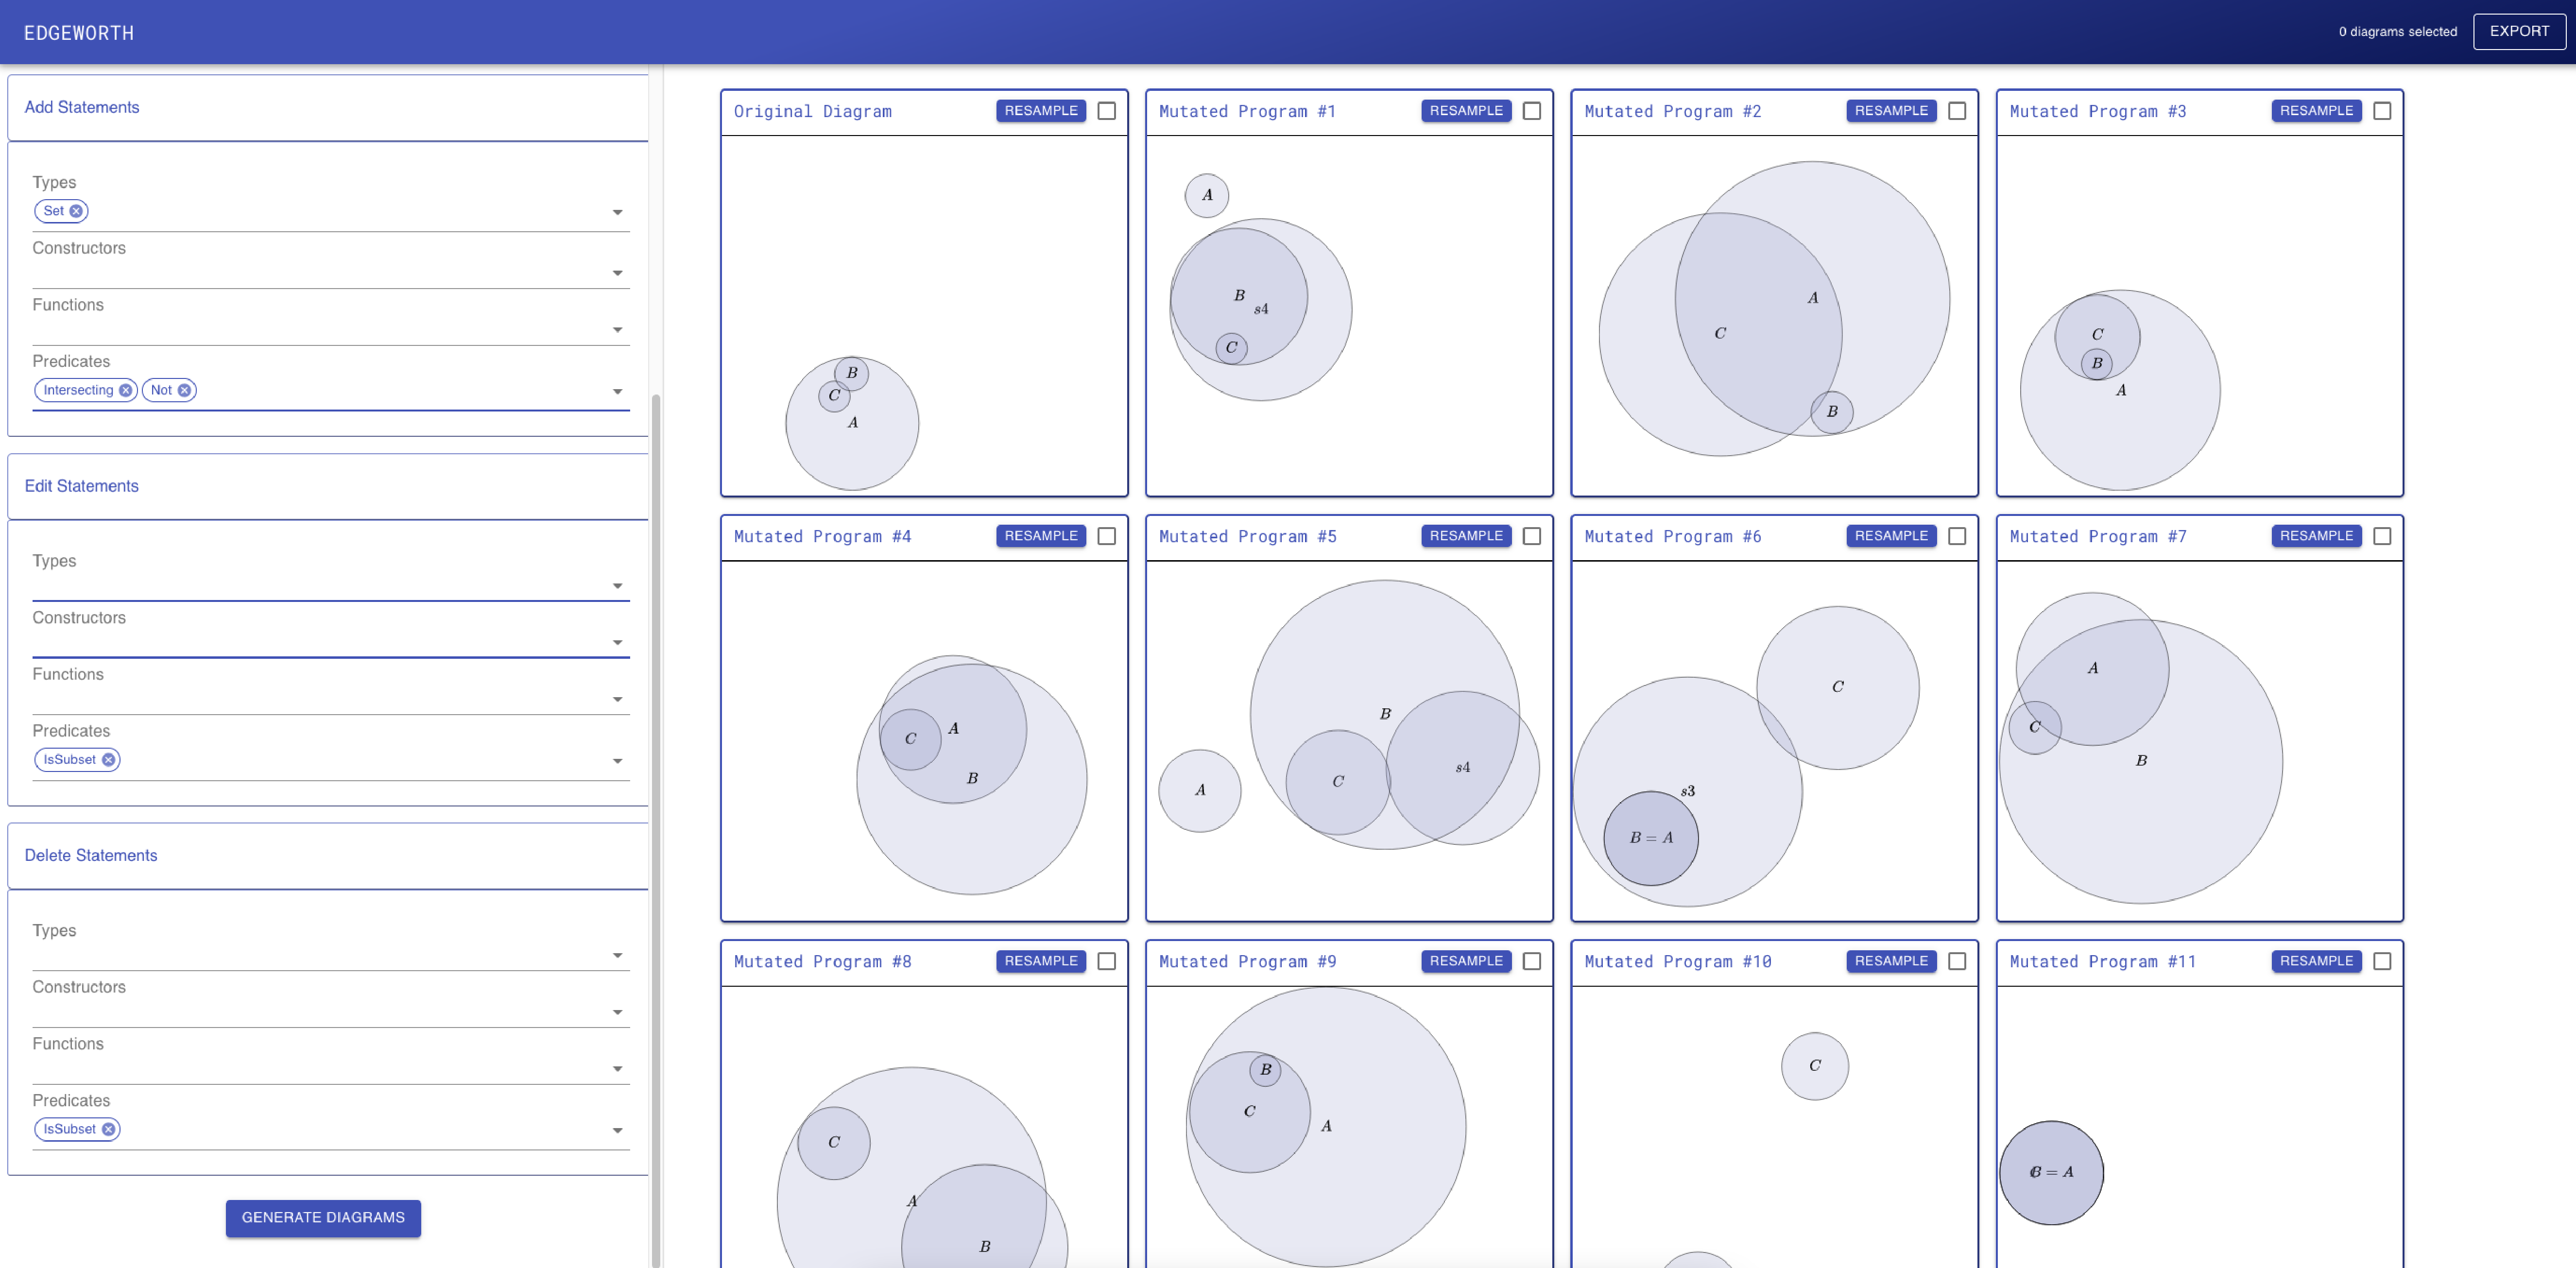
\includegraphics[width=\linewidth]{assets/appendix/edgeworth-bad-output.pdf}
    \caption{A screenshot of the \Edgeworth interface, after generating examples for a translation problem focusing on improper subsets. Because of the configuration, pool of mutant diagrams aren't suitable for this problem.}
    \label{fig:edgeworth-bad-output}
\end{figure}


With the \Edgeworth mutator, the primary mode of interaction is configuration-based: the author creates a mutator configuration and the mutator generates a set of diagrams. When these diagrams don't satisfy the needs of the author (\eg missing counterexamples that are important for an educational goal), the author can only edit the configuration again and hope to get better ones. In short, the quality of \Edgeworth-generated diagrams are sensitive to the configuration. 

For example, suppose an author would like to create translation problems that test students' knowledge of improper subsets, especially the fact that if $A \subseteq B$, $A = B$ is allowed. Using the \Edgeworth mutator, the author first creates a prompt \Substance program:

\begin{verbatim}
Set A, B, C
IsSubSet(B, A)
IsSubset(C, A)
\end{verbatim}

Not familiar with how program mutator works, the author picks a few options in the configuration interface and clicks ``Generate Diagrams.'' Ideally, \Edgeworth should generate a set of examples of the subset relations that include the edge cases of $A = B$, $A = C$, or $B = C$, and counterexamples of $B \not\subseteq A$ or $C \not\subseteq A$. 

However, the output from \Edgeworth seems too random (\cref{fig:edgeworth-bad-output}). There are useful counterexamples, but none of the diagrams include edge cases such as:
\begin{verbatim}
Set A, B, C
IsSubSet(B, A)
IsSubset(C, A)
Equal(B, C)
\end{verbatim}

In other words, without intimate knowledge of how the \Edgeworth mutator is configured, the author cannot express their intent easily. In this case, it's much more natural to write a few examples from scratch, or manually make slight tweaks to examples in the mutant pool. I propose to \textbf{create a programming-by-example (PBE) workflow, where the author manually creates or edits a few diagrams, and \Edgeworth generates more diagrams with similar properties.}

Using this workflow for the example above, the author can manually create a few examples by directly editing the prompt program. In this case, the author adds the \sub{Equal(B, C)} predicate. Their intent is to include the edge case of improper subsets in this problem, where some of the subset relations are actually equality. \Edgeworth generates a set of similar examples that add \sub{Equal} predicates with existing identifiers in different ways. 

\vspace{10pt}
\begin{figure}[h]
    \centering
    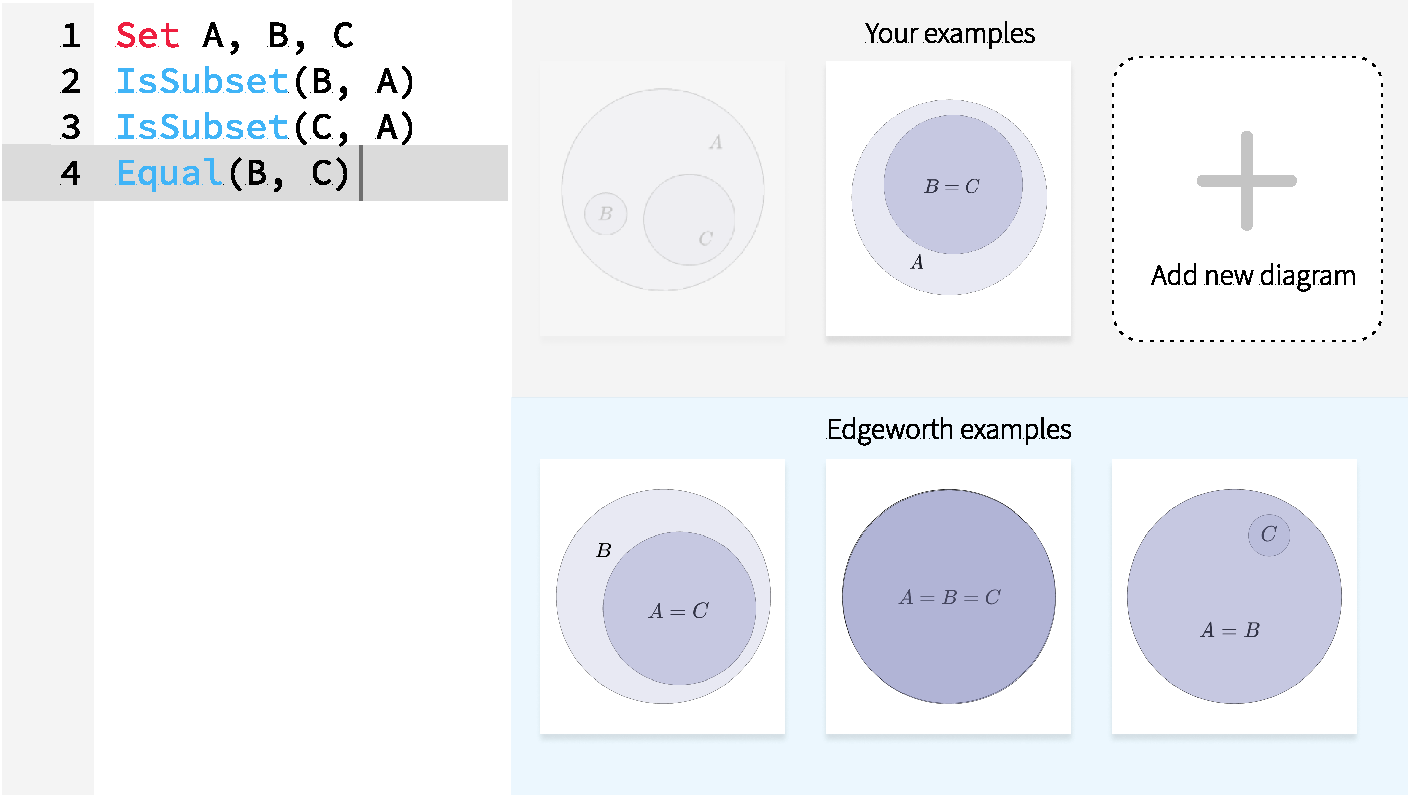
\includegraphics[width=0.8\linewidth]{assets/appendix/synthesis-driven-workflow.pdf}
    % \caption{Caption}
    % \label{fig:my_label}
\end{figure}
\vspace{10pt}

The addition of \sub{Equal(B, C)} is effectively a user-generated mutation, and \Edgeworth needs to understand this mutation to generate similar instances. To do so, the \Edgeworth synthesizer matches a series of author edits to predefined mutations. Once the synthesizer finds a mutation path that describes the author edit, it can then inform the mutator to generate examples with similar properties (\ie including the edge case of equal sets). Using this workflow, the author can rapidly author diagrams that belong to a particular category in the translation problem. For example, the problem below has diagrams that include set equalities as correct answers, and diagrams that violate one or both subset relations as incorrect answers.

\vspace{10pt}
\begin{figure}[h]
    \centering
    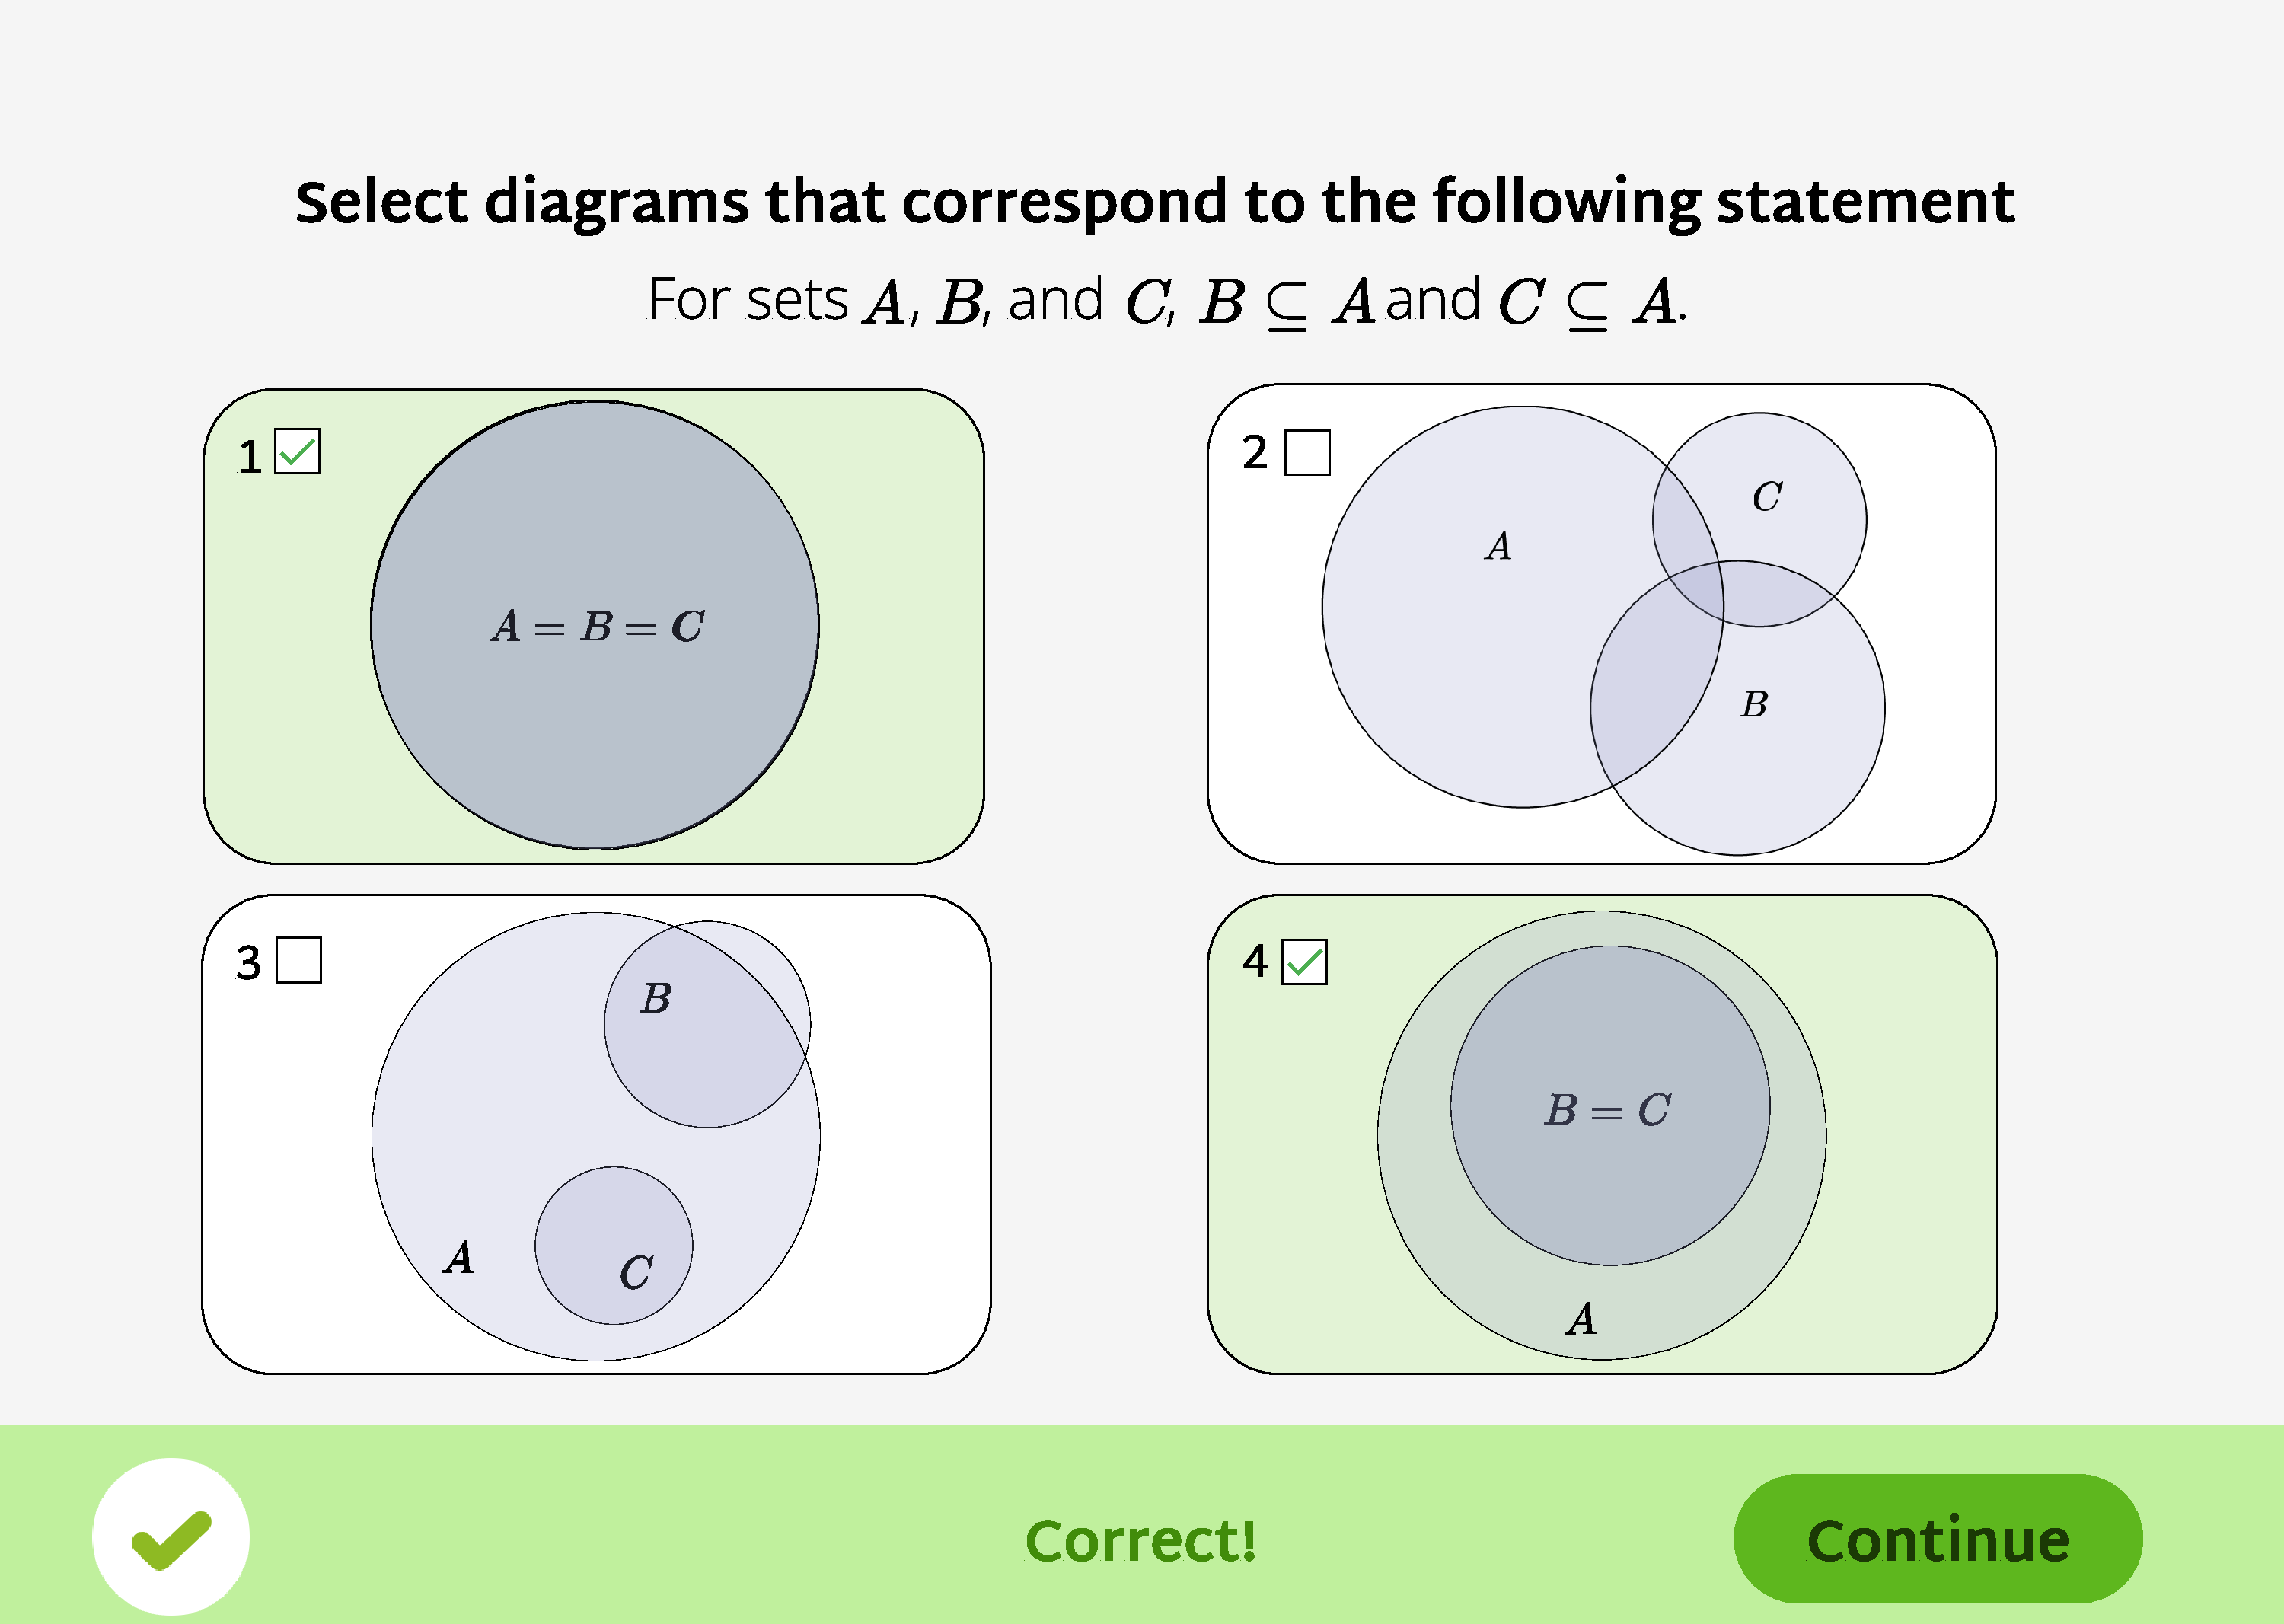
\includegraphics[width=0.8\linewidth]{assets/appendix/translation-problem-sets.pdf}
    % \caption{Caption}
    % \label{fig:my_label}
\end{figure}
\vspace{10pt}

\subsection{Automatic detection of examples and counterexamples}
\label{sec:autodetect}

One key application of \Edgeworth is generating translation problems with examples and counterexamples. Therefore, it's important for the system to understand whether a diagram is an example or counterexample of the prompt. However, the \Edgeworth mutator performs \Substance program mutations on the prompt without knowing if a mutant is semantically equivalent to the prompt. To address this, I propose to \textbf{automatically detect examples and counterexamples}.

One heuristic is cross-instance energy evaluation (CIEE) described in~\cref{sec:mutation}.  CIEE determines the distance between two \Substance programs by examining visual constraint satisfaction. 

Another approach is to provide the \Edgeworth mutator with more semantic information such that it generates examples and counterexamples by construction. Currently, none of the mutation operators carry any mathematical semantics because \Domain doesn't contain enough information. For instance, many mathematical predicates have reflexive, symmetric, transitive, and substitution properties, but \Domain only encodes basic type definitions. For a more precise notion of correctness, I plan to extend \Domain to model such properties, and use them in the \Edgeworth mutator, possibly together with CIEE, to generate higher quality mutants.  

\subsection{Hypotheses and research questions}

Comparing with related work discussed in \cref{sec:edgeworth-related}, \Edgeworth uniquely support scalable generation of diagrammatic translation problems in multiple domains. Therefore, in this section, I discuss hypotheses that cover the essential features of \Edgeworth such as the mutation-based approach and automatic detection of examples and counterexamples. For each hypothesis, I will also discuss further research questions to be investigated in the evaluation plan. 

\boxtext{\textbf{H1:} Given manageable effort in configuring the mutator, \Edgeworth can reliably generate examples and counterexamples for translation problems with relatively few mutants required.}

An effective translation problem needs to include both examples and counterexamples. Therefore, the technical approach of \Edgeworth---program mutations on \Substance code---must produce them reliably. To verify H1, the following research questions need to be answered:

\begin{itemize}
    \item \textbf{R1.1}: How many mutants does \Edgeworth need to generate to obtain sufficient examples and counterexamples for translation problems?
    \item \textbf{R1.2}: How frequently does \Edgeworth succeed or fail at doing so?
\end{itemize}

The preliminary evaluation showed that the mutator configuration will affect the quality of the mutants. Therefore, I will also address the following research question on mutator configuration and will use the results to further investigate possible ways to lower the configuration burden, e.g. the programming-by-example workflow and changes to the configuration format.

\begin{itemize}
    \item \textbf{R1.3}: How much configuration effort is required to produce examples and counterexamples? 
\end{itemize}

\boxtext{\textbf{H2}: \Edgeworth makes translation problem authoring more efficient.}

The main goal of \Edgeworth is to improve the efficiency of translation problem authoring. To verify H2, the evaluation plan will answer:
\begin{itemize}
    \item  \textbf{R2.1}: Comparing with workflows that authors are using, can \Edgeworth shorten the authoring time of translation problems?
    \item  \textbf{R2.2}: Which aspect(s) of the authoring workflow does \Edgeworth simplify, and does \Edgeworth introduce new authoring difficulties? 
    \item  \textbf{R2.3}: Are authors more efficient using the configuration-based workflow or programming-by-example workflow?
\end{itemize}

Regardless of the answer to R2.1, meaningful results on R2.2 can provide more insights on how \Edgeworth's approach impacts the problem authoring experience. For instance, I postulate that \Edgeworth improves authoring efficiency by (1) simplifying the mechanics of diagram production and (2) reducing the author's effort to come up with examples and counterexamples. On the other hand, \Edgeworth's mutation-based approach may introduce new problems such as difficulties finding the right diagrams from the mutant pool and controlling the quality of examples. The automatic detection heuristics described above aim to mitigate these difficulties.

\boxtext{\textbf{H3}: \Edgeworth can automatically distinguish examples from counterexamples, and this feature helps authors find examples and counterexamples for translation problems.}

The effectiveness of translation problems depends on the choice of examples and counterexamples. I hypothesize that example generation/selection is a nontrivial activity that authors spend time doing, and computational support in \Edgeworth can help authors identify examples/counterexamples. Answering the following research questions will verify H3:

\begin{itemize}
    \item \textbf{R3.1}: Can \Edgeworth automatically detect examples, counterexamples, and edge cases with a reasonably high accuracy?
    \item \textbf{R3.2}: Do the detection results help authors identify potential answers to translation problems?
\end{itemize}

\section{Evaluation plan}

\subsection{Pilot usability evaluation}

To prepare the \Edgeworth prototype for evaluation, I will first evaluate the usability of \Edgeworth by recruiting authors to perform small authoring tasks with the \Edgeworth prototype. For example, the participants may be asked to author a simple diagrammatic translation problem. The goal of this pilot study is to identify missing features, usability problems, and opportunities for simplification. The study may include several rounds with increasingly high-fidelity prototypes. After each round, I will refine the design and implement the next prototype. Here are some possible high-level questions for the study:
\begin{itemize}
    \item What are the key design considerations for translation problem authoring? How do they fit with the features of \Edgeworth?
    \item How do authors prefer to work with \Edgeworth? When do they opt to write a configuration file and generate many diagrams? When do they use the by-example workflow? Do they mix the two workflows?
    \item How does the experience compare to their existing tools? How can \Edgeworth incorporate useful parts of them? 
\end{itemize}

\subsection{Technical evaluation of automated production of diagram problems}
\label{sec:case-study}

While the preliminary study (\cref{sec:edgeworth-prelim-eval}) shows some promise of \Edgeworth's approach, the data from this study is insufficient for investigating H1 and R1.1-3. In this study, I will investigate if \Edgeworth can reliably produce diagrams for translation problems (H1) by gathering richer data on its success rate, efficiency, and human effort. 

\subsubsection{Translation problem set} 

I will reproduce diagrammatic problems from the same geometry textbook~\cite{holtGeometry} used in \cref{sec:edgeworth-prelim-eval}. In the textbook, diagrammatic problems often require representational fluency but aren't presented as multiple-choice translation problems with diagrams as choices. I plan to start with the original set of 24 translation problems that were reframed from textbook problems, and potentially extend the dataset using the same methodology of reframing the problems. Each translation problem in the dataset will include (1) a textual prompt, (2) four diagrams, and (3) a \Substance prompt program.

\subsubsection{Data collection} 

The output of \Edgeworth may be sensitive to factors like randomness of mutation paths and quality of configuration. Therefore, for each of the translation problems in the dataset, I will use the configuration-based workflow (\cref{sec:mutation}) in \Edgeworth to produce multiple problem instances. Each valid problem instance is a multiple-choice translation problem with four diagrams comprised of examples, counterexamples, and edge cases of the problem prompt. The validity of problem instances is determined manually during the study. 

Each problem instance may take multiple trials of executing the mutator and editing the configuration. The authoring process for each problem instance will be screen-recorded and documented. \Edgeworth will also be instrumented to log data such as the following:

\begin{itemize}
    \item Mutator data: mutant diagrams and their mutation paths, number of mutant generated per trial.
    \item Execution history: configuration file per execution and mutants selected for the translation problem.
    \item Edit history of the configuration: edits to a configuration for a particular translation problem and changes to configuration schema between translation problems.
\end{itemize}

\subsubsection{Proposed methodology} 

For R1.1, I plan to count (1) the number of mutants generated over multiple trials to obtain a valid problem instance and (2) the number of mutants in the last successful trial. The average of (2) over all translation problems measures the reliability of \Edgeworth given a good configuration, whereas that of (1) factors in the human effort of authoring such a configuration. To answer R1.2, I will run \Edgeworth with the configuration of the last successful trial, and measure the success rate of producing valid problem instances. 

For R1.3, I will use the screen recording to measure the time-to-completion for each valid problem instance and also count trials-to-completion. These data may be subject to particular contexts in which I will run the study. To gain a more objective understanding of the complexity of configuration files, I will also measure the specificity of the configuration to help answer R1.3. As a base case, an empty configuration with defaults takes no human effort to author, and a configuration that selects many constructs from \Domain takes significantly more effort. I will use the edit history and the length of the resulting configuration file itself to measure configuration effort.

% As discussed in \cref{sec:definitions}, while it's straightforward to distinguish between examples and counterexamples
The validity of edge cases depends on the context of a particular translation problem.  For all of the problems, I will label examples, counterexamples, and edge cases, and document the context and my rationale.  In addition, I will recruit a geometry teacher to label a sample of the problems from the dataset. I will then calculate the inter-rater reliability of between my rating and the teacher rating to assess whether my rating agrees with expert judgments. 

Then, I will use \Edgeworth to perform automatic detection (\cref{sec:autodetect}) on all translation problems from this study, and compute inter-rater reliability between the manual labels and detection results. Along with the documented edge case decisions from the study, a high inter-rater reliability can provide more confidence that \Edgeworth can accurately detect positive and negative edge cases (R3.1). 

\subsection{Experimental evaluation of authoring efficiency}

This study is an authoring experiment that compares (1) \Edgeworth against existing authoring tools and (2) features of \Edgeworth (\eg configuration vs. PBD, auto-detection on/off). Participants will create diagrammatic translation problems using conventional drawing tools or \Edgeworth. For H2, this study quantitatively measures the efficiency with or without \Edgeworth, compare between configuration-based and PBD workflows, and gather qualitative data on how \Edgeworth improves and/or hinders translation problem authoring. For H3, this study will test within-subjects whether the automatic detection feature helps participants in distinguishing and generating examples and counterexamples. 

\subsubsection{Tasks}

All participants will be asked to complete 4 translation problem authoring tasks, each sampled from the case study dataset (see \cref{sec:case-study}). For each task, the participant will be given (1) an textual problem prompt and (2) an example diagram (\ie a correct response to the prompt). Participants will create 3 instances of this problem, each with two examples and counterexamples (12 diagrams in total). In the participant is using \Edgeworth, they will also be given (3) a \Penrose trio corresponding to the prompt. 

\subsubsection{Proposed methodology}

The participants will be divided into 3 groups, each group distinguished by the tool being used: 
\begin{itemize}
    \item Control group: a conventional drawing tool\footnote{During recruitment, we will survey the participants to find a common tool they know}, \eg Google Drawings
    \item \Edgeworth-config group: \Edgeworth with the configuration-based interface
    \item \Edgeworth-PBD group: \Edgeworth with the PBD interface
\end{itemize}
For both \Edgeworth groups, the automatic detection feature will be enabled for 50\% of the tasks. Below is an example of the study setup, where D indicates \Edgeworth with automatic detection and N without.

\begin{table}[h]
\centering
\begin{tabular}{l|cccccc}
                    & Task 1 & Task 2 & Task 3 & Task 4  \\ \hline
Control             &   -    &    -   &    -   &   -   \\ 
\Edgeworth-config 1 & N      & D      & D      & N   \\
\Edgeworth-config 2 & D      & N      & D      & N   \\
\Edgeworth-PBD 1    & D      & N      & N      & D   \\
\Edgeworth-PBD 2    & N      & D      & N      & D   \\
\end{tabular}
\end{table}
Between tasks, participants will be asked to explain how they came up with examples and counterexamples, identified useful edge cases, and interacted with the authoring tool. The study sessions will be recorded and transcribed. 

The recording and \Edgeworth data will be analyzed to measure the authoring time for each task. The total authoring time difference between the conventional drawing tool and \Edgeworth will be used to answer R2.1. The time difference between \Edgeworth-config and \Edgeworth-PBD will answer R2.3. I will also observe the relative time participants spend on writing configuration in \Edgeworth-config and \Substance code in \Edgeworth-PBD. This observation will provide an estimate of the overhead of each workflow. Finally, I will compare the time with or without automatic detection (R3.2). 

If participants do spend less time with automatic detection enabled, there may be two possible sources of this speedup: (1) they can filter down mutant diagrams in \Edgeworth more quickly, \ie less tool interaction; (2) \Edgeworth helps offload the effort in identifying examples and counterexamples, \ie less example ideation. Participants' answers between tasks will help us determine which of these reasons is dominant (R2.2).

The video recordings will be coded to identify challenges participants encounter in both the conventional drawing tool and configuration-based or PBD \Edgeworth (R2.2, R2.3), and how they interact with the automatic detection result (R3.2). 

\section{Milestones and timeline}

\cref{fig:timeline} shows a plan for the sequence of the proposed work mapped to a timeline.

\vspace{10pt}
\begin{figure}[h]
\begin{center}
\begin{ganttchart}[y unit title=0.4cm,
y unit chart=0.5cm,
x unit=0.32cm,
vgrid,hgrid, 
title label anchor/.style={below=-1.6ex},
title left shift=.05,
title right shift=-.05,
title height=1,
progress label text={},
bar height=0.7,
group right shift=0,
group top shift=.6,
group height=.3]{1}{40}
%labels
\gantttitle{Fall 22}{11} 
\gantttitle{Spring 23}{11} 
\gantttitle{Summer 23}{7} 
\gantttitle{Fall 23}{11} 
\\
%tasks
\ganttbar{Usability Pilot}{1}{1} \\
\ganttgroup{System Impl.}{1}{16} \\
\ganttbar{Config system}{1}{4} \\
\ganttbar{PBD system}{9}{16} \\
\ganttgroup{Technical eval.}{3}{12} \\
\ganttbar{Dataset}{3}{4} \\
\ganttbar{Experiment}{5}{8} \\
\ganttbar{Analysis}{9}{10} \\
\ganttbar{Writeup}{11}{12} \\
\ganttgroup{Experimental eval.}{12}{28} \\
\ganttbar{Authoring Pilot}{15}{16} \\
\ganttbar{IRB \& Design}{12}{16} \\
\ganttbar{Recruitment}{14}{16} \\
\ganttbar{Experiment}{17}{23} \\
\ganttbar{Analysis}{24}{25} \\
\ganttbar{Writeup}{26}{28} \\
\ganttgroup{Dissertation}{29}{40} \\
\ganttbar{Drafting}{29}{36} \\
\ganttmilestone{Defense}{40}
% \ganttbar{task 3}{9}{10} \\
% \ganttbar{task 4}{11}{15} \\
% \ganttbar[progress=33]{task 5}{20}{22} \\
% \ganttbar{task 6}{18}{19} \\
% \ganttbar{task 7}{16}{18} \\
% \ganttbar[progress=0]{task 8}{21}{24}

% %relations 
% \ganttlink{elem1}{elem2} 
% \ganttlink{elem3}{elem4} 
% \ganttlink{elem1}{elem5} 
% \ganttlink{elem3}{elem5} 
% \ganttlink{elem2}{elem6} 
% \ganttlink{elem3}{elem6} 
% \ganttlink{elem5}{elem7} 
\end{ganttchart}
\end{center}
\caption{Timeline of \Edgeworth projects}
\label{fig:timeline}
\end{figure}


% I will compare the time it takes participants to create content and the quality of the content. 
% I will recruit previous formative participants for this study and draw from the formative participant pool if needed.

\backmatter

\renewcommand{\baselinestretch}{1.0}\normalsize

% By default \bibsection is \chapter*, but we really want this to show
% up in the table of contents and pdf bookmarks.
% \renewcommand{\bibsection}{\chapter{\bibname}}
%\renewcommand{\bibpreamble}{This text goes between the ``Bibliography''
%  header and the actual list of references}
% \bibliographystyle{thesis-style}
% \bibliography{zotero} %your bib file

% Make sure the bibliography appears in the table of contents
\cleardoublepage
% Print the bibliography with a chapter heading
\printbibliography[heading=bibintoc]
% \bibliographystyle{thesis-style}


\end{document}
